% !TeX program = xelatex
\documentclass[12pt,a4paper,oneside]{report}
\usepackage{fontspec}
\usepackage{pdfpages}
\usepackage[margin=1in]{geometry}
\usepackage{microtype,setspace}
\usepackage{amsmath,amssymb,booktabs,array,longtable,tabularx,multirow,graphicx,float,pdflscape}
\usepackage[british]{babel}
\usepackage{csquotes}
\usepackage[backend=biber,style=apa,natbib=true,sortcites=true]{biblatex}
\addbibresource{references.bib}
\addbibresource{references_additions.bib}
\usepackage{xcolor,xurl,enumitem,caption,subcaption}
\usepackage[hidelinks,unicode]{hyperref}
% Set \thesisdraftfalse here for a copy without the DRAFT watermark.
\newif\ifthesisdraft
\thesisdrafttrue
\ifthesisdraft
  \AddToHook{shipout/foreground}{%
    \put(.5\paperwidth,-.5\paperheight){%
      \makebox[0pt][c]{\raisebox{-.5\height}{%
        
\includegraphics[width=.70\paperwidth]{figures/draft-watermark.pdf}}}}}
\fi
\captionsetup{labelfont=bf,textfont=it,labelsep=newline,justification=raggedright,singlelinecheck=false,position=top}
\newcommand{\displaynote}[1]{\par\smallskip\begingroup\raggedright\small\noindent\textit{Note.}
#1\par\endgroup}
\setlength{\bibhang}{0.5in}
\usepackage{fancyhdr}
\setlength{\headheight}{15pt}
\pagestyle{fancy}\fancyhf{}\fancyhead[L]{\small\nouppercase{\leftmark}}\fancyfoot[C]{\thepage}
\renewcommand{\headrulewidth}{0.3pt}
\setlength{\emergencystretch}{3em}
% Shared thesis typography. Author-requested editorial layout, 26 November 2026.
% Document class, fonts, paper, margins and APA bibliography style stay in the roots.
\RequirePackage{etoolbox}

\onehalfspacing
\setlength{\parskip}{0pt}
\setlength{\parindent}{6mm}
\newcommand{\apaprose}{%
  \onehalfspacing\raggedright
  \setlength{\parindent}{6mm}\setlength{\parskip}{0pt}}
\AtBeginEnvironment{longtable}{\singlespacing}

% Moderate, positive physical gaps. Keep report.cls fonts, numbering and
% no-break behavior. Its negative before-skip convention suppresses first-
% paragraph indentation; it does not place text in a negative vertical gap.
\makeatletter
\newcommand{\ThesisSpacingPatchFailed}{%
  \PackageError{thesis-formatting}{Unexpected report.cls heading definition}%
    {Check the shared heading-spacing patches against the document class.}}
\patchcmd{\@makechapterhead}{\vspace*{50\p@}}{\vspace*{24\p@}}{}{\ThesisSpacingPatchFailed}
\patchcmd{\@makechapterhead}{\vskip 20\p@}{\vskip 12\p@}{}{\ThesisSpacingPatchFailed}
\patchcmd{\@makechapterhead}{\vskip 40\p@}{\vskip 24\p@}{}{\ThesisSpacingPatchFailed}
\patchcmd{\@makeschapterhead}{\vspace*{50\p@}}{\vspace*{24\p@}}{}{\ThesisSpacingPatchFailed}
\patchcmd{\@makeschapterhead}{\vskip 40\p@}{\vskip 24\p@}{}{\ThesisSpacingPatchFailed}
\patchcmd{\section}{-3.5ex \@plus -1ex \@minus -.2ex}%
  {-2.5ex \@plus -.8ex \@minus -.2ex}{}{\ThesisSpacingPatchFailed}
\patchcmd{\section}{2.3ex \@plus.2ex}%
  {1.4ex \@plus.2ex}{}{\ThesisSpacingPatchFailed}
\patchcmd{\subsection}{-3.25ex\@plus -1ex \@minus -.2ex}%
  {-2.25ex\@plus -.8ex \@minus -.2ex}{}{\ThesisSpacingPatchFailed}
\patchcmd{\subsection}{1.5ex \@plus .2ex}%
  {1ex \@plus .2ex}{}{\ThesisSpacingPatchFailed}
\patchcmd{\subsubsection}{-3.25ex\@plus -1ex \@minus -.2ex}%
  {-2ex\@plus -.8ex \@minus -.2ex}{}{\ThesisSpacingPatchFailed}
\patchcmd{\subsubsection}{1.5ex \@plus .2ex}%
  {.8ex \@plus .2ex}{}{\ThesisSpacingPatchFailed}

% A centered abstract heading shared by all editions; no negative offsets.
\newcommand{\ThesisAbstractHeading}{%
  \begingroup
  \renewcommand{\@makeschapterhead}[1]{%
    \vspace*{12\p@}%
    {\parindent\z@\centering\normalfont\interlinepenalty\@M
     \Huge\bfseries ##1\par\nobreak\vskip18\p@}}%
  \chapter*{Abstract}%
  \endgroup}
\makeatother

% Float contents and footnotes retain setspace's single-spacing behavior.
% Keep figure/table definitions and caption typography unchanged.
\setlength{\textfloatsep}{14pt plus 2pt minus 4pt}
\setlength{\intextsep}{10pt plus 2pt minus 2pt}
\setlength{\floatsep}{10pt plus 2pt minus 2pt}

% Avoid isolated first/last paragraph lines without changing authored text.
\clubpenalty=10000
\widowpenalty=10000
\displaywidowpenalty=10000

% Permit a readable large float to share a page with surrounding prose.
\renewcommand{\topfraction}{.85}
\renewcommand{\bottomfraction}{.75}
\renewcommand{\textfraction}{.1}
\renewcommand{\floatpagefraction}{.7}

% Editable literature-review objects shared by the thesis and review editions.
\newcommand{\ThesisLiteratureEmbedded}{}
% !TeX program = xelatex
% Compile from the thesis root for a standalone proof.
%
% To use the objects independently in the thesis, put these two lines in
% the shared preamble before \begin{document} (adjust the input path if needed):
%   \newcommand{\ThesisLiteratureEmbedded}{}
%   % !TeX program = xelatex
% Compile from the thesis root for a standalone proof.
%
% To use the objects independently in the thesis, put these two lines in
% the shared preamble before \begin{document} (adjust the input path if needed):
%   \newcommand{\ThesisLiteratureEmbedded}{}
%   \input{figures/review_figure_table.tex}
% Then place \ReviewDepthFigure and \ReviewFollowupTable at their respective
% locations in Chapter 2. Cross-references: fig:review-depth, tab:literature-synthesis.
% The thesis already loads fontspec, geometry, setspace, array, tabularx,
% booktabs, float, caption and biblatex. Its caption and font settings apply.
%
% The values describe the original appraisal records. Changing the question
% to coverage in the full papers would require recoding before using it here.
\ifdefined\ThesisLiteratureEmbedded\else
  \documentclass[12pt,a4paper,oneside]{report}
  \usepackage{fontspec}
  \usepackage[margin=1in]{geometry}
  \usepackage{setspace,array,tabularx,longtable,booktabs,float,caption}
  \captionsetup{labelfont=bf,textfont=it,labelsep=newline,
    justification=raggedright,singlelinecheck=false,position=top}
  % Use neutral preview numbering. The thesis supplies its own numbers.
  \pagestyle{empty}
\fi
\input{figures/tikz_style.tex}
% The 9 bp annotation size needs supported script sizes for TikZ's math setup.
\DeclareMathSizes{9bp}{9bp}{7pt}{5pt}

% DATA -----------------------------------------------------------------------
% Arguments: topic ID, label, direct test, used/discussed, no record, unclear.
% One status per topic per appraisal; a work can contribute to several topics.
% The figure and table both read this block.
\newcommand{\ReviewAppraisalN}{94}
\newcommand{\ReviewTopics}[1]{%
  #1{inputs}{Adding an input}{46}{15}{30}{3}%
  #1{rule}{Choice of fusion rule}{37}{28}{29}{0}%
  #1{training}{Training strategy}{28}{60}{4}{2}%
  #1{noise}{Corrupted inputs at test}{21}{22}{50}{1}%
  #1{encoding}{Input representation}{15}{67}{7}{5}%
  #1{absent}{Missing inputs at inference}{11}{15}{68}{0}%
  #1{shift}{Transfer across settings}{11}{30}{52}{1}%
}
\newcommand{\ReviewPercent}[1]{%
  \begingroup
  \pgfmathparse{100*(#1)/\ReviewAppraisalN}%
  \pgfmathprintnumber[fixed,precision=1,fixed zerofill]{\pgfmathresult}\%%
  \endgroup}
\newcommand{\ReviewCheckRow}[6]{%
  \ifnum\numexpr #3+#4+#5+#6\relax=\ReviewAppraisalN\relax\else
    \PackageError{review-visuals}{Counts for #1 must sum to \ReviewAppraisalN}%
      {Check the four status counts in the ReviewTopics block.}%
  \fi}
\ReviewTopics{\ReviewCheckRow}

% Native author-year citations in the thesis; the stand-alone proof prints
% the same work identities without needing references.bib or a Biber run.
\newcommand{\ReviewCite}[2]{%
  \ifcsname parencite\endcsname\parencite{#1}\else(#2)\fi}
\newcommand{\ReviewNote}[1]{%
  \par\smallskip\begingroup\small\raggedright\noindent\textit{Note.} #1\par\endgroup}

% FIGURE ---------------------------------------------------------------------
% Coordinates are fractions of the current text width; row spacing is in cm.
% Greyscale fills and hatching remain distinguishable in monochrome print.
\newcount\ReviewRowIndex
\newcommand{\ReviewBarRow}[6]{%
  \advance\ReviewRowIndex by 1\relax
  \pgfmathsetmacro{\ReviewY}{-0.72*\the\ReviewRowIndex}%
  \pgfmathsetmacro{\ReviewA}{\ReviewLeft+\ReviewWidth*(#3)/\ReviewAppraisalN}%
  \pgfmathsetmacro{\ReviewB}{\ReviewLeft+\ReviewWidth*(#3+#4)/\ReviewAppraisalN}%
  \pgfmathsetmacro{\ReviewC}{\ReviewLeft+\ReviewWidth*(#3+#4+#5)/\ReviewAppraisalN}%
  \node[anchor=west] at (0,\ReviewY) {#2};
  \path[fill=black!76] (\ReviewLeft,{\ReviewY-.18}) rectangle (\ReviewA,{\ReviewY+.18});
  \path[fill=black!36] (\ReviewA,{\ReviewY-.18}) rectangle (\ReviewB,{\ReviewY+.18});
  \path[fill=white] (\ReviewB,{\ReviewY-.18}) rectangle (\ReviewC,{\ReviewY+.18});
  \ifnum#6>0\relax
    \begin{scope}
      \clip (\ReviewC,{\ReviewY-.18}) rectangle (\ReviewRight,{\ReviewY+.18});
      \pgfmathtruncatemacro{\ReviewHatches}{ceil((\ReviewRight-\ReviewC)/.008)+3}%
      \foreach \j in {0,...,\ReviewHatches} {
        \draw[black!75,line width=.28pt]
          ({\ReviewC-.020+.008*\j},{\ReviewY-.18}) --
          ({\ReviewC+.002+.008*\j},{\ReviewY+.18});
      }
    \end{scope}
    \draw[black!55,line width=.25pt] (\ReviewC,{\ReviewY-.18}) -- (\ReviewC,{\ReviewY+.18});
  \fi
  \draw[black!65,line width=.3pt] (\ReviewLeft,{\ReviewY-.18}) rectangle (\ReviewRight,{\ReviewY+.18});
  \node at (.745,\ReviewY) {#3}; \node at (.818,\ReviewY) {#4};
  \node at (.889,\ReviewY) {#5}; \node at (.958,\ReviewY) {#6};
}
\newcommand{\ReviewKey}[1]{%
  \tikz[baseline=-.5ex,x=1pt,y=1pt]{%
    \ifcase#1\relax\or \fill[black!76] (0,0) rectangle (11,6);
    \or \fill[black!36] (0,0) rectangle (11,6);
    \or \fill[white] (0,0) rectangle (11,6);
    \or \begin{scope}\clip (0,0) rectangle (11,6);
      \foreach \j in {-6,-3,0,3,6,9}{\draw[line width=.3pt] (\j,0)--++(6,6);}
    \end{scope}\fi
    \draw[black!65,line width=.3pt] (0,0) rectangle (11,6);}}
\newcommand{\ReviewDepthFigure}{%
  \begin{figure}[H]
    \centering\singlespacing
    \caption{Depth of investigation recorded in the \ReviewAppraisalN{} literature appraisals}
    \label{fig:review-depth}
    \begingroup\fontsize{9bp}{11bp}\selectfont
    \begin{tabular}{@{}l@{\hspace{2em}}l@{}}
      \ReviewKey{1}\enspace Direct test recorded &
      \ReviewKey{2}\enspace Used or discussed only\\[2pt]
      \ReviewKey{3}\enspace No treatment recorded &
      \ReviewKey{4}\enspace Unclear from appraisal
    \end{tabular}\par\medskip
    \begin{tikzpicture}[x=\linewidth,y=1cm,
      every node/.style={thesis label,inner sep=0pt,outer sep=0pt}]
      \path[use as bounding box] (0,-5.36) rectangle (1,.78);
      \def\ReviewLeft{.300}\def\ReviewWidth{.388}\def\ReviewRight{.688}
      \node[anchor=west,thesis panel label] at (0,.53) {Topic};
      \node[thesis panel label] at (.494,.53) {Share of appraisals};
      \node[thesis panel label] at (.854,.53) {Number of appraisals};
      \foreach \tick in {0,25,50,75,100}{
        \pgfmathsetmacro{\xx}{\ReviewLeft+\ReviewWidth*\tick/100}
        \node[thesis annotation] at (\xx,.05) {\tick\%};
        \draw[black!20,line width=.25pt] (\xx,-.20) -- (\xx,-5.36);
      }
      \node[thesis annotation] at (.745,.05) {Test};
      \node[thesis annotation] at (.818,.05) {Use};
      \node[thesis annotation] at (.889,.05) {None};
      \node[thesis annotation] at (.958,.05) {Unclear};
      \ReviewRowIndex=0\relax
      \ReviewTopics{\ReviewBarRow}
    \end{tikzpicture}
    \endgroup
    \ReviewNote{Each topic uses all \ReviewAppraisalN{} appraisals as its denominator.
      A paper can contribute to several topics. A direct test requires a recorded
      comparison or intervention. ``No treatment recorded'' describes what the
      author's appraisal documents; it does not establish that the paper omitted
      the topic. The four categories record the depth documented in the appraisals.}
  \end{figure}}

% TABLE ----------------------------------------------------------------------
% Each topic has two editable cells: recorded finding and author-proposed
% follow-up. Citation keys in the first argument of ReviewCite are those used
% in the thesis bibliography. The second argument is the stand-alone fallback.
\newcommand{\ReviewText}[3]{%
  \expandafter\def\csname ReviewFinding#1\endcsname{#2}%
  \expandafter\def\csname ReviewQuestion#1\endcsname{#3}}
\ReviewText{inputs}
  {Image and audio fusion gained 5.9 percentage points over image alone in four-state
   welding classification. In weld penetration, each single input tied fusion on the
   clean test. Adding gripper state reduced accuracy in handover
   \ReviewCite{P003,Hua2026Weld,Thoduka2024Handover}{Fan et al., 2026; Hua et al., 2026; Thoduka et al., 2024}.
   Each contrast applies to its own outcome, inputs and assessment cases.}
  {Does a second input improve on the strongest single input when both are tested on the same held-out runs?}
\ReviewText{rule}
  {An RGB--3D inspection study compared a static mean with a learned gate using complete inputs
   \ReviewCite{P026}{Deng et al., 2026}. A gated unit outperformed concatenation on a
   movie-genre task. Some alternative multimodal tool-wear pipelines were weaker
   than the visual reference, although the proposed model improved on it
   \ReviewCite{P006,P045}{Arevalo et al., 2017; Zhang et al., 2026}.
   Differences in encoders or fitting can change the ranking. The genre result has
   no direct industrial validation.}
  {Under which faults does a learned rule outperform a static rule after both receive the same exposure during training?}
\ReviewText{training}
  {Both models had 1.02\% error on clean digits. With two quadrants missing, modality-dropout training reduced error from 35.91\% to 7.19\%
   \ReviewCite{P005}{Neverova et al., 2015}. This controlled digit comparison tests
   exposure to specified absence patterns, not performance under industrial outages.}
  {How much of a gain under corruption comes from training exposure, and how much from the fusion rule?}
\ReviewText{noise}
  {One bearing study compared fusion rules at 0~dB. Another reported the proposed model's accuracy when one input was degraded
   \ReviewCite{Huang2026Rolling,P046}{Huang \& Tong, 2026; Sun et al., 2026}.
   Their corruption conditions and controls differ; the proposed model's corrupted
   accuracy alone does not establish incremental fusion benefit.}
  {At the same fault severity, does fusion outperform both the intact input and a static combination?}
\ReviewText{encoding}
  {Hand-crafted geometry can support 3D inspection, temporal patches retain useful
   information for forecasting, and learned video features address action recognition
   \ReviewCite{Horwitz2023Back,Nie2023PatchTST,P013}{Horwitz \& Hoshen, 2023; Nie et al., 2023; Liu et al., 2022}.
   The tasks and supervision differ. These studies do not rank the representations
   on the same target.}
  {Which encoding adds complementary information when the target, observation window and fitting budget are fixed?}
\ReviewText{absent}
  {A pressure-only student was trained for single-input deployment; modality-resilient
   inspection and RGB--geometry inspection also examine incomplete inputs
   \ReviewCite{Li2025PGMTKD,Xu2025ModalityResilient,P026}{Li et al., 2025; Xu et al., 2025; Deng et al., 2026}.
   A planned input restriction leaves performance under sudden loss or partial
   corruption open. Simulated dropout and inference-time absence require distinct
   assessment conditions.}
  {Does a policy trained for a known missing stream also cope with an unexpected outage during operation?}
\ReviewText{shift}
  {Handover was tested across robots. A bearing study used target-domain validation during transfer
   \ReviewCite{Thoduka2024Handover,Huang2026Rolling}{Thoduka et al., 2024; Huang \& Tong, 2026}.
   Inspection methods were reapplied to Eyecandies with target-specific normal memories
   \ReviewCite{P026,P033}{Deng et al., 2026; Xu et al., 2026}.
   Rebuilding those memories uses target data. Performance of an unchanged predictor
   at a new installation remains a separate question.}
  {How much fusion benefit persists on a new machine or site when access to target data is controlled?}
\ReviewText{credibility}
  {Participant-disjoint assessment tests performance on held-out people. Selection
   and calibration also affect what a reported score measures
   \ReviewCite{Thoduka2024Handover,P004,Guo2017Calibration}{Thoduka et al., 2024; Varma \& Simon, 2006; Guo et al., 2017}.
   Independence depends on the physical grouping. Accuracy alone gives neither
   failure ranking nor probability quality.}
  {Does the apparent benefit persist with appropriate grouping, training-side selection
   and calibration, and assessment of ranking and probability quality?}
\newcommand{\ReviewTableRow}[6]{%
  \textbf{#2} &
  \csname ReviewFinding#1\endcsname & \csname ReviewQuestion#1\endcsname\tabularnewline
  \addlinespace[.45em]}
\newcommand{\ReviewFollowupTable}{%
    \begingroup\small\singlespacing
    \setlength{\tabcolsep}{4.5pt}
    \renewcommand{\arraystretch}{1.04}
    \begin{longtable}{@{}>{\raggedright\arraybackslash}p{.18\linewidth}
      >{\raggedright\arraybackslash}p{.47\linewidth}
      >{\raggedright\arraybackslash}p{.31\linewidth}@{}}
      \caption{Findings, limits and follow-up questions from the literature review}
      \label{tab:literature-synthesis}\\
      \toprule
      \textbf{Topic or question} & \textbf{Published finding and its limit}
        & \textbf{Follow-up question}\\
      \midrule
      \endfirsthead
      \caption[]{Findings, limits and follow-up questions from the literature review (continued)}\\
      \toprule
      \textbf{Topic or question} & \textbf{Published finding and its limit}
        & \textbf{Follow-up question}\\
      \midrule
      \endhead
      \midrule
      \multicolumn{3}{r@{}}{\footnotesize Continued on the next page}\\
      \endfoot
      \bottomrule
      \endlastfoot
      \ReviewTopics{\ReviewTableRow}
      \textbf{How credible is the estimate?} &
      \ReviewFindingcredibility & \ReviewQuestioncredibility\tabularnewline
    \end{longtable}
    \endgroup
}

% Stand-alone preview only. In the thesis, each object is placed by its macro.
\ifdefined\ThesisLiteratureEmbedded
  \expandafter\endinput
\fi
\begin{document}
\ReviewDepthFigure
\clearpage
\ReviewFollowupTable
\end{document}

% Then place \ReviewDepthFigure and \ReviewFollowupTable at their respective
% locations in Chapter 2. Cross-references: fig:review-depth, tab:literature-synthesis.
% The thesis already loads fontspec, geometry, setspace, array, tabularx,
% booktabs, float, caption and biblatex. Its caption and font settings apply.
%
% The values describe the original appraisal records. Changing the question
% to coverage in the full papers would require recoding before using it here.
\ifdefined\ThesisLiteratureEmbedded\else
  \documentclass[12pt,a4paper,oneside]{report}
  \usepackage{fontspec}
  \usepackage[margin=1in]{geometry}
  \usepackage{setspace,array,tabularx,longtable,booktabs,float,caption}
  \captionsetup{labelfont=bf,textfont=it,labelsep=newline,
    justification=raggedright,singlelinecheck=false,position=top}
  % Use neutral preview numbering. The thesis supplies its own numbers.
  \pagestyle{empty}
\fi
% Input from a LaTeX preamble, with the working directory at the thesis root.
\RequirePackage{tikz}

% Shared semantic palette. See VISUAL_STYLE.md for the role definitions.
\definecolor{ThesisVision}{HTML}{0072B2}
\definecolor{ThesisSensor}{HTML}{009E73}
\definecolor{ThesisContext}{HTML}{56B4E9}
\definecolor{ThesisFusion}{HTML}{CC79A7}
\definecolor{ThesisBaseline}{HTML}{595959}
\definecolor{ThesisHighlight}{HTML}{E69F00}
\definecolor{ThesisAudio}{HTML}{882255}
\definecolor{ThesisThermal}{HTML}{D55E00}
\definecolor{ThesisDepth}{HTML}{332288}
\definecolor{ThesisVibration}{HTML}{117733}
\definecolor{ThesisWrench}{HTML}{999933}
\definecolor{ThesisInk}{HTML}{222222}

\tikzset{
  thesis label/.style={
    font=\normalfont\fontsize{10bp}{12bp}\selectfont,
    text=ThesisInk
  },
  thesis annotation/.style={
    thesis label,
    font=\normalfont\fontsize{9bp}{11bp}\selectfont
  },
  thesis panel label/.style={
    thesis label,
    font=\normalfont\bfseries\fontsize{11bp}{13bp}\selectfont
  },
  thesis box/.style={
    thesis label,
    rectangle, rounded corners=3bp, line width=0.8bp,
    inner xsep=6bp, inner ysep=4bp, align=center
  },
  module/.style={
    thesis box, draw=ThesisBaseline, fill=white
  },
  fusion/.style={
    module, draw=ThesisFusion, fill=ThesisFusion!12!white, line width=1.2bp,
    font=\normalfont\bfseries\fontsize{10bp}{12bp}\selectfont
  },
  data/.style={
    thesis box, draw=#1, fill=#1!12!white
  },
  data/.default=ThesisSensor,
  arrow/.style={
    -stealth, draw=ThesisInk, line width=0.8bp, line cap=round,
    shorten >=1bp, shorten <=1bp
  },
  groupbox/.style={
    thesis box, draw=ThesisBaseline, dashed, inner sep=8bp
  }
}

% The 9 bp annotation size needs supported script sizes for TikZ's math setup.
\DeclareMathSizes{9bp}{9bp}{7pt}{5pt}

% DATA -----------------------------------------------------------------------
% Arguments: topic ID, label, direct test, used/discussed, no record, unclear.
% One status per topic per appraisal; a work can contribute to several topics.
% The figure and table both read this block.
\newcommand{\ReviewAppraisalN}{94}
\newcommand{\ReviewTopics}[1]{%
  #1{inputs}{Adding an input}{46}{15}{30}{3}%
  #1{rule}{Choice of fusion rule}{37}{28}{29}{0}%
  #1{training}{Training strategy}{28}{60}{4}{2}%
  #1{noise}{Corrupted inputs at test}{21}{22}{50}{1}%
  #1{encoding}{Input representation}{15}{67}{7}{5}%
  #1{absent}{Missing inputs at inference}{11}{15}{68}{0}%
  #1{shift}{Transfer across settings}{11}{30}{52}{1}%
}
\newcommand{\ReviewPercent}[1]{%
  \begingroup
  \pgfmathparse{100*(#1)/\ReviewAppraisalN}%
  \pgfmathprintnumber[fixed,precision=1,fixed zerofill]{\pgfmathresult}\%%
  \endgroup}
\newcommand{\ReviewCheckRow}[6]{%
  \ifnum\numexpr #3+#4+#5+#6\relax=\ReviewAppraisalN\relax\else
    \PackageError{review-visuals}{Counts for #1 must sum to \ReviewAppraisalN}%
      {Check the four status counts in the ReviewTopics block.}%
  \fi}
\ReviewTopics{\ReviewCheckRow}

% Native author-year citations in the thesis; the stand-alone proof prints
% the same work identities without needing references.bib or a Biber run.
\newcommand{\ReviewCite}[2]{%
  \ifcsname parencite\endcsname\parencite{#1}\else(#2)\fi}
\newcommand{\ReviewNote}[1]{%
  \par\smallskip\begingroup\small\raggedright\noindent\textit{Note.} #1\par\endgroup}

% FIGURE ---------------------------------------------------------------------
% Coordinates are fractions of the current text width; row spacing is in cm.
% Greyscale fills and hatching remain distinguishable in monochrome print.
\newcount\ReviewRowIndex
\newcommand{\ReviewBarRow}[6]{%
  \advance\ReviewRowIndex by 1\relax
  \pgfmathsetmacro{\ReviewY}{-0.72*\the\ReviewRowIndex}%
  \pgfmathsetmacro{\ReviewA}{\ReviewLeft+\ReviewWidth*(#3)/\ReviewAppraisalN}%
  \pgfmathsetmacro{\ReviewB}{\ReviewLeft+\ReviewWidth*(#3+#4)/\ReviewAppraisalN}%
  \pgfmathsetmacro{\ReviewC}{\ReviewLeft+\ReviewWidth*(#3+#4+#5)/\ReviewAppraisalN}%
  \node[anchor=west] at (0,\ReviewY) {#2};
  \path[fill=black!76] (\ReviewLeft,{\ReviewY-.18}) rectangle (\ReviewA,{\ReviewY+.18});
  \path[fill=black!36] (\ReviewA,{\ReviewY-.18}) rectangle (\ReviewB,{\ReviewY+.18});
  \path[fill=white] (\ReviewB,{\ReviewY-.18}) rectangle (\ReviewC,{\ReviewY+.18});
  \ifnum#6>0\relax
    \begin{scope}
      \clip (\ReviewC,{\ReviewY-.18}) rectangle (\ReviewRight,{\ReviewY+.18});
      \pgfmathtruncatemacro{\ReviewHatches}{ceil((\ReviewRight-\ReviewC)/.008)+3}%
      \foreach \j in {0,...,\ReviewHatches} {
        \draw[black!75,line width=.28pt]
          ({\ReviewC-.020+.008*\j},{\ReviewY-.18}) --
          ({\ReviewC+.002+.008*\j},{\ReviewY+.18});
      }
    \end{scope}
    \draw[black!55,line width=.25pt] (\ReviewC,{\ReviewY-.18}) -- (\ReviewC,{\ReviewY+.18});
  \fi
  \draw[black!65,line width=.3pt] (\ReviewLeft,{\ReviewY-.18}) rectangle (\ReviewRight,{\ReviewY+.18});
  \node at (.745,\ReviewY) {#3}; \node at (.818,\ReviewY) {#4};
  \node at (.889,\ReviewY) {#5}; \node at (.958,\ReviewY) {#6};
}
\newcommand{\ReviewKey}[1]{%
  \tikz[baseline=-.5ex,x=1pt,y=1pt]{%
    \ifcase#1\relax\or \fill[black!76] (0,0) rectangle (11,6);
    \or \fill[black!36] (0,0) rectangle (11,6);
    \or \fill[white] (0,0) rectangle (11,6);
    \or \begin{scope}\clip (0,0) rectangle (11,6);
      \foreach \j in {-6,-3,0,3,6,9}{\draw[line width=.3pt] (\j,0)--++(6,6);}
    \end{scope}\fi
    \draw[black!65,line width=.3pt] (0,0) rectangle (11,6);}}
\newcommand{\ReviewDepthFigure}{%
  \begin{figure}[H]
    \centering\singlespacing
    \caption{Depth of investigation recorded in the \ReviewAppraisalN{} literature appraisals}
    \label{fig:review-depth}
    \begingroup\fontsize{9bp}{11bp}\selectfont
    \begin{tabular}{@{}l@{\hspace{2em}}l@{}}
      \ReviewKey{1}\enspace Direct test recorded &
      \ReviewKey{2}\enspace Used or discussed only\\[2pt]
      \ReviewKey{3}\enspace No treatment recorded &
      \ReviewKey{4}\enspace Unclear from appraisal
    \end{tabular}\par\medskip
    \begin{tikzpicture}[x=\linewidth,y=1cm,
      every node/.style={thesis label,inner sep=0pt,outer sep=0pt}]
      \path[use as bounding box] (0,-5.36) rectangle (1,.78);
      \def\ReviewLeft{.300}\def\ReviewWidth{.388}\def\ReviewRight{.688}
      \node[anchor=west,thesis panel label] at (0,.53) {Topic};
      \node[thesis panel label] at (.494,.53) {Share of appraisals};
      \node[thesis panel label] at (.854,.53) {Number of appraisals};
      \foreach \tick in {0,25,50,75,100}{
        \pgfmathsetmacro{\xx}{\ReviewLeft+\ReviewWidth*\tick/100}
        \node[thesis annotation] at (\xx,.05) {\tick\%};
        \draw[black!20,line width=.25pt] (\xx,-.20) -- (\xx,-5.36);
      }
      \node[thesis annotation] at (.745,.05) {Test};
      \node[thesis annotation] at (.818,.05) {Use};
      \node[thesis annotation] at (.889,.05) {None};
      \node[thesis annotation] at (.958,.05) {Unclear};
      \ReviewRowIndex=0\relax
      \ReviewTopics{\ReviewBarRow}
    \end{tikzpicture}
    \endgroup
    \ReviewNote{Each topic uses all \ReviewAppraisalN{} appraisals as its denominator.
      A paper can contribute to several topics. A direct test requires a recorded
      comparison or intervention. ``No treatment recorded'' describes what the
      author's appraisal documents; it does not establish that the paper omitted
      the topic. The four categories record the depth documented in the appraisals.}
  \end{figure}}

% TABLE ----------------------------------------------------------------------
% Each topic has two editable cells: recorded finding and author-proposed
% follow-up. Citation keys in the first argument of ReviewCite are those used
% in the thesis bibliography. The second argument is the stand-alone fallback.
\newcommand{\ReviewText}[3]{%
  \expandafter\def\csname ReviewFinding#1\endcsname{#2}%
  \expandafter\def\csname ReviewQuestion#1\endcsname{#3}}
\ReviewText{inputs}
  {Image and audio fusion gained 5.9 percentage points over image alone in four-state
   welding classification. In weld penetration, each single input tied fusion on the
   clean test. Adding gripper state reduced accuracy in handover
   \ReviewCite{P003,Hua2026Weld,Thoduka2024Handover}{Fan et al., 2026; Hua et al., 2026; Thoduka et al., 2024}.
   Each contrast applies to its own outcome, inputs and assessment cases.}
  {Does a second input improve on the strongest single input when both are tested on the same held-out runs?}
\ReviewText{rule}
  {An RGB--3D inspection study compared a static mean with a learned gate using complete inputs
   \ReviewCite{P026}{Deng et al., 2026}. A gated unit outperformed concatenation on a
   movie-genre task. Some alternative multimodal tool-wear pipelines were weaker
   than the visual reference, although the proposed model improved on it
   \ReviewCite{P006,P045}{Arevalo et al., 2017; Zhang et al., 2026}.
   Differences in encoders or fitting can change the ranking. The genre result has
   no direct industrial validation.}
  {Under which faults does a learned rule outperform a static rule after both receive the same exposure during training?}
\ReviewText{training}
  {Both models had 1.02\% error on clean digits. With two quadrants missing, modality-dropout training reduced error from 35.91\% to 7.19\%
   \ReviewCite{P005}{Neverova et al., 2015}. This controlled digit comparison tests
   exposure to specified absence patterns, not performance under industrial outages.}
  {How much of a gain under corruption comes from training exposure, and how much from the fusion rule?}
\ReviewText{noise}
  {One bearing study compared fusion rules at 0~dB. Another reported the proposed model's accuracy when one input was degraded
   \ReviewCite{Huang2026Rolling,P046}{Huang \& Tong, 2026; Sun et al., 2026}.
   Their corruption conditions and controls differ; the proposed model's corrupted
   accuracy alone does not establish incremental fusion benefit.}
  {At the same fault severity, does fusion outperform both the intact input and a static combination?}
\ReviewText{encoding}
  {Hand-crafted geometry can support 3D inspection, temporal patches retain useful
   information for forecasting, and learned video features address action recognition
   \ReviewCite{Horwitz2023Back,Nie2023PatchTST,P013}{Horwitz \& Hoshen, 2023; Nie et al., 2023; Liu et al., 2022}.
   The tasks and supervision differ. These studies do not rank the representations
   on the same target.}
  {Which encoding adds complementary information when the target, observation window and fitting budget are fixed?}
\ReviewText{absent}
  {A pressure-only student was trained for single-input deployment; modality-resilient
   inspection and RGB--geometry inspection also examine incomplete inputs
   \ReviewCite{Li2025PGMTKD,Xu2025ModalityResilient,P026}{Li et al., 2025; Xu et al., 2025; Deng et al., 2026}.
   A planned input restriction leaves performance under sudden loss or partial
   corruption open. Simulated dropout and inference-time absence require distinct
   assessment conditions.}
  {Does a policy trained for a known missing stream also cope with an unexpected outage during operation?}
\ReviewText{shift}
  {Handover was tested across robots. A bearing study used target-domain validation during transfer
   \ReviewCite{Thoduka2024Handover,Huang2026Rolling}{Thoduka et al., 2024; Huang \& Tong, 2026}.
   Inspection methods were reapplied to Eyecandies with target-specific normal memories
   \ReviewCite{P026,P033}{Deng et al., 2026; Xu et al., 2026}.
   Rebuilding those memories uses target data. Performance of an unchanged predictor
   at a new installation remains a separate question.}
  {How much fusion benefit persists on a new machine or site when access to target data is controlled?}
\ReviewText{credibility}
  {Participant-disjoint assessment tests performance on held-out people. Selection
   and calibration also affect what a reported score measures
   \ReviewCite{Thoduka2024Handover,P004,Guo2017Calibration}{Thoduka et al., 2024; Varma \& Simon, 2006; Guo et al., 2017}.
   Independence depends on the physical grouping. Accuracy alone gives neither
   failure ranking nor probability quality.}
  {Does the apparent benefit persist with appropriate grouping, training-side selection
   and calibration, and assessment of ranking and probability quality?}
\newcommand{\ReviewTableRow}[6]{%
  \textbf{#2} &
  \csname ReviewFinding#1\endcsname & \csname ReviewQuestion#1\endcsname\tabularnewline
  \addlinespace[.45em]}
\newcommand{\ReviewFollowupTable}{%
    \begingroup\small\singlespacing
    \setlength{\tabcolsep}{4.5pt}
    \renewcommand{\arraystretch}{1.04}
    \begin{longtable}{@{}>{\raggedright\arraybackslash}p{.18\linewidth}
      >{\raggedright\arraybackslash}p{.47\linewidth}
      >{\raggedright\arraybackslash}p{.31\linewidth}@{}}
      \caption{Findings, limits and follow-up questions from the literature review}
      \label{tab:literature-synthesis}\\
      \toprule
      \textbf{Topic or question} & \textbf{Published finding and its limit}
        & \textbf{Follow-up question}\\
      \midrule
      \endfirsthead
      \caption[]{Findings, limits and follow-up questions from the literature review (continued)}\\
      \toprule
      \textbf{Topic or question} & \textbf{Published finding and its limit}
        & \textbf{Follow-up question}\\
      \midrule
      \endhead
      \midrule
      \multicolumn{3}{r@{}}{\footnotesize Continued on the next page}\\
      \endfoot
      \bottomrule
      \endlastfoot
      \ReviewTopics{\ReviewTableRow}
      \textbf{How credible is the estimate?} &
      \ReviewFindingcredibility & \ReviewQuestioncredibility\tabularnewline
    \end{longtable}
    \endgroup
}

% Stand-alone preview only. In the thesis, each object is placed by its macro.
\ifdefined\ThesisLiteratureEmbedded
  \expandafter\endinput
\fi
\begin{document}
\ReviewDepthFigure
\clearpage
\ReviewFollowupTable
\end{document}


\setcounter{tocdepth}{2}\setcounter{secnumdepth}{2}
\newcolumntype{P}[1]{>{\raggedright\arraybackslash}p{#1}}
\newcolumntype{Y}{>{\raggedright\arraybackslash}X}
% The register is read in the preamble so each URL can be entered literally.
% Keep each EvidenceFile declaration on its own line. A URL may contain a
% percent-encoded path, an underscore, a query string, or a line fragment.
\ExplSyntaxOn
\prop_new:N \g_thesis_evidence_urls_prop
\prop_new:N \g_thesis_evidence_names_prop
\seq_new:N \g_thesis_evidence_rows_seq
\seq_new:N \l_thesis_evidence_note_seq
\NewDocumentCommand{\EvidenceFile}{m m m v}
  {
    \prop_if_in:NnTF \g_thesis_evidence_urls_prop {#1}
      { \PackageError{thesis-evidence}{Duplicate~file~ID~#1}{} }
      {
        \tl_set:Nx \l_tmpa_tl { \tl_trim_spaces:n {#4} }
        \tl_if_empty:NF \l_tmpa_tl
          {
            % Match the complete HTTPS GitHub origin and an owner/repository.
            % Reject lookalike hosts, credentials, ports and embedded whitespace.
            \exp_args:NnV \regex_match:nnF
              { \A [Hh][Tt][Tt][Pp][Ss] :// [Gg][Ii][Tt][Hh][Uu][Bb][.][Cc][Oo][Mm]/
                [^/\s?\x{23}]+ / [^/\s?\x{23}]+ (?: [/?\x{23}] [^\s]* )? \Z }
              \l_tmpa_tl
              {
                \PackageWarningNoLine{thesis-evidence}{Ignoring~non-GitHub~or~invalid~URL~for~#1}
                \tl_clear:N \l_tmpa_tl
              }
          }
        \prop_gput:NnV \g_thesis_evidence_urls_prop {#1} \l_tmpa_tl
        \prop_gput:Nnn \g_thesis_evidence_names_prop {#1} {#3}
        \seq_gput_right:Nn \g_thesis_evidence_rows_seq
          { \EvidenceTableRow{#1}{#2}{#3} }
      }
  }
\NewDocumentCommand{\EvidenceExternal}{m}
  {
    \prop_get:NnNTF \g_thesis_evidence_urls_prop {#1} \l_tmpa_tl
      {
        \tl_if_empty:NTF \l_tmpa_tl
          { Link~unavailable }
          { \exp_args:NV \href \l_tmpa_tl {Link~here} }
      }
      { \PackageError{thesis-evidence}{Unknown~file~ID~#1}{} }
  }
\NewDocumentCommand{\EvidenceDestination}{m}
  {
    \prop_get:NnNTF \g_thesis_evidence_urls_prop {#1} \l_tmpa_tl
      {
        \tl_if_empty:NTF \l_tmpa_tl
          { \hyperlink{evidence-#1}{#1} }
          { \bool_if:NTF \g_thesis_evidence_footnotes_bool
              { \exp_args:NV \href \l_tmpa_tl {#1} }
              { \hyperlink{evidence-#1}{#1} } }
      }
      { \PackageError{thesis-evidence}{Unknown~file~ID~#1}{} }
  }
\NewDocumentCommand{\PrintEvidenceRows}{}
  { \seq_use:Nn \g_thesis_evidence_rows_seq {} }
% Publication URLs may be recorded without changing reviewed chapter layout.
% Existing \ev calls are opt-in; \ev* renders one explicitly reviewed note.
\bool_new:N \g_thesis_evidence_footnotes_bool
\NewDocumentCommand{\EnableEvidenceFootnotes}{}
  { \bool_gset_true:N \g_thesis_evidence_footnotes_bool }
\NewDocumentCommand{\DisableEvidenceFootnotes}{}
  { \bool_gset_false:N \g_thesis_evidence_footnotes_bool }
\cs_new_protected:Npn \thesis_evidence_note_link:nnn #1#2#3
  {
    \prop_get:NnN \g_thesis_evidence_urls_prop {#1} \l_tmpa_tl
    \prop_get:NnN \g_thesis_evidence_names_prop {#1} \l_tmpb_tl
    \tl_if_blank:nTF {#2}
      { \exp_args:NV \href \l_tmpa_tl { \exp_args:NV \nolinkurl \l_tmpb_tl } }
      { \exp_args:NV \href \l_tmpa_tl {#2} }
    ~[\hyperlink{evidence-#1}{#1}]
    \tl_if_blank:nF {#3} {~(#3)}
  }
\cs_new_protected:Npn \thesis_evidence_collect:nnn #1#2#3
  {
    \prop_get:NnNTF \g_thesis_evidence_urls_prop {#1} \l_tmpa_tl
      {
        \tl_if_empty:NF \l_tmpa_tl
          {
            \seq_if_in:NnF \l_thesis_evidence_note_seq
              { \thesis_evidence_note_link:nnn {#1}{#2}{#3} }
              { \seq_put_right:Nn \l_thesis_evidence_note_seq
                  { \thesis_evidence_note_link:nnn {#1}{#2}{#3} } }
          }
      }
      { \PackageError{thesis-evidence}{Unknown~file~ID~#1}{} }
  }
\cs_new_protected:Npn \thesis_evidence_render_note:nn #1#2
  {
    \group_begin:
      \seq_clear:N \l_thesis_evidence_note_seq
      % Old \EvidenceRef{ID}{pinpoint} remains valid; role is optional.
      \RenewDocumentCommand{\EvidenceRef}{O{} m m}
        { \thesis_evidence_collect:nnn {##2}{##1}{##3} }
      \clist_map_inline:nn {#2} {##1}
      \seq_if_empty:NF \l_thesis_evidence_note_seq
        { \footnote{\raggedright #1:~\seq_use:Nn \l_thesis_evidence_note_seq {;~}} }
    \group_end:
  }
\NewDocumentCommand{\ev}{s m m}
  {
    \IfBooleanTF{#1}
      { \thesis_evidence_render_note:nn {#2}{#3} }
      { \bool_if:NT \g_thesis_evidence_footnotes_bool
          { \thesis_evidence_render_note:nn {#2}{#3} } }
  }
\ExplSyntaxOff
\newcommand{\EvidenceTableRow}[3]{%
  \hypertarget{evidence-#1}{#1} & #2 & \nolinkurl{#3} & \EvidenceExternal{#1}\\}
\NewDocumentCommand{\EvidenceRef}{O{} m m}{%
  \if\relax\detokenize{#1}\relax\else#1~\fi
  \EvidenceDestination{#2}%
  \if\relax\detokenize{#3}\relax\else\space(#3)\fi}
% One slot per source file or separately identified dated copy.
% Replace the empty pipes with |the exact GitHub file URL|. Keep one declaration per line.
% IDs are persistent. Add new sources under new IDs without renumbering existing entries.
% The companion evidence_source_index.csv identifies each relative source path.
\EvidenceFile{E001}{Study design}{01_EXPOSE_ALIGNMENT_DECISION.md}||
\EvidenceFile{E002}{Study design}{01_ORIGINAL_EXPOSE.pdf}||
\EvidenceFile{E003}{Study design}{02_THESIS_BASELINE_REPORT.md}||
\EvidenceFile{E004}{Study design}{02_THESIS_WRITING_MAP_v3.md}||
\EvidenceFile{E005}{Literature}{additional_web_search_log.json}||
\EvidenceFile{E006}{Literature}{candidate_screening.csv}||
\EvidenceFile{E007}{Literature}{evidence.json}||
\EvidenceFile{E008}{Literature}{quote_audit.json}||
\EvidenceFile{E009}{Literature}{web_search_log.json}||
\EvidenceFile{E010}{Literature}{appraisal_P001_P020.json}||
\EvidenceFile{E011}{Literature}{appraisal_P021_P040.json}||
\EvidenceFile{E012}{Literature}{appraisal_P041_P059.json}||
\EvidenceFile{E013}{Literature}{expanded_comparison_matrix.csv}||
\EvidenceFile{E014}{Literature}{expanded_comparison_matrix.json}||
\EvidenceFile{E015}{Literature}{original37_literature_matrix.csv}||
\EvidenceFile{E016}{Literature}{review_counts.json}||
\EvidenceFile{E017}{Literature}{identity_catalog.json}||
\EvidenceFile{E018}{Intel Welding}{foundations.json}||
\EvidenceFile{E019}{Intel Welding}{04_foundations.py}||
\EvidenceFile{E020}{PHM}{active_scope.md}|https://github.com/Parth-0804/pi-multimodal-ad/blob/e2037412036c5bbfc01fb2323215a37ef0b2e090/docs/active_scope.md|
\EvidenceFile{E021}{PHM}{HANDOFF.md}||
\EvidenceFile{E022}{PHM}{FINAL_CLAIM_MATRIX.md}|https://github.com/Parth-0804/pi-multimodal-ad/blob/e2037412036c5bbfc01fb2323215a37ef0b2e090/implementations/general/docs/thesis/FINAL_CLAIM_MATRIX.md|
\EvidenceFile{E023}{PHM}{TARGET_VERSION_LEDGER.md}|https://github.com/Parth-0804/pi-multimodal-ad/blob/e2037412036c5bbfc01fb2323215a37ef0b2e090/implementations/PHM2026/docs/studies/TARGET_VERSION_LEDGER.md|
\EvidenceFile{E024}{PHM}{KNOWN_IMPLEMENTATION_ISSUES.md}|https://github.com/Parth-0804/pi-multimodal-ad/blob/e2037412036c5bbfc01fb2323215a37ef0b2e090/implementations/PHM2026/experiments/walkthrough/01_rtdetr_scalar_regression/KNOWN_IMPLEMENTATION_ISSUES.md|
\EvidenceFile{E025}{PHM}{experiments/phm2026/README.md}||
\EvidenceFile{E026}{PHM}{loeo_summary.csv}||
\EvidenceFile{E027}{PHM}{resolved_config.yaml}|https://github.com/Parth-0804/pi-multimodal-ad/blob/e2037412036c5bbfc01fb2323215a37ef0b2e090/implementations/PHM2026/results/runs/phm2026_patchtst_baseline/20260912T053924941825Z-4235307c/config/resolved_config.yaml|
\EvidenceFile{E028}{PHM}{loeo_evaluation.py}|https://github.com/Parth-0804/pi-multimodal-ad/blob/e2037412036c5bbfc01fb2323215a37ef0b2e090/implementations/PHM2026/scripts/results/loeo_evaluation.py|
\EvidenceFile{E029}{PHM}{sq2_sq3_fusion.py}|https://github.com/Parth-0804/pi-multimodal-ad/blob/e2037412036c5bbfc01fb2323215a37ef0b2e090/implementations/PHM2026/scripts/results/sq2_sq3_fusion.py|
\EvidenceFile{E030}{PHM}{modality_fusion.py}|https://github.com/Parth-0804/pi-multimodal-ad/blob/e2037412036c5bbfc01fb2323215a37ef0b2e090/implementations/PHM2026/src/phm2026/fusion/modality_fusion.py|
\EvidenceFile{E031}{PHM}{model.py}|https://github.com/Parth-0804/pi-multimodal-ad/blob/e2037412036c5bbfc01fb2323215a37ef0b2e090/implementations/PHM2026/src/phm2026/models/patchtst/model.py|
\EvidenceFile{E032}{PHM}{patchtst/regression.py}|https://github.com/Parth-0804/pi-multimodal-ad/blob/e2037412036c5bbfc01fb2323215a37ef0b2e090/implementations/PHM2026/src/phm2026/models/patchtst/regression.py|
\EvidenceFile{E033}{PHM}{rtdetr/regression.py}|https://github.com/Parth-0804/pi-multimodal-ad/blob/e2037412036c5bbfc01fb2323215a37ef0b2e090/implementations/PHM2026/src/phm2026/models/rtdetr/regression.py|
\EvidenceFile{E034}{PHM}{src/phm2026/README.md}|https://github.com/Parth-0804/pi-multimodal-ad/blob/e2037412036c5bbfc01fb2323215a37ef0b2e090/implementations/PHM2026/src/phm2026/README.md|
\EvidenceFile{E035}{PHM}{image_damage.py}|https://github.com/Parth-0804/pi-multimodal-ad/blob/e2037412036c5bbfc01fb2323215a37ef0b2e090/implementations/PHM2026/src/phm2026/targets/image_damage.py|
\EvidenceFile{E036}{PHM}{final_baseline_rtdetr/REPORT.md}|https://github.com/Parth-0804/pi-multimodal-ad/blob/e2037412036c5bbfc01fb2323215a37ef0b2e090/implementations/PHM2026/docs/tutorials/final_baseline_rtdetr/REPORT.md|
\EvidenceFile{E037}{PHM}{patchtst_freq_baseline/REPORT.md}|https://github.com/Parth-0804/pi-multimodal-ad/blob/e2037412036c5bbfc01fb2323215a37ef0b2e090/implementations/PHM2026/docs/tutorials/patchtst_freq_baseline/REPORT.md|
\EvidenceFile{E038}{REASSEMBLE}{per_condition_metrics.csv}||
\EvidenceFile{E039}{REASSEMBLE}{metrics.csv}||
\EvidenceFile{E040}{REASSEMBLE}{ADDITIONAL_IMPROVEMENTS_EXECUTED_HANDOFF.md}||
\EvidenceFile{E041}{REASSEMBLE}{AUDIO_FEASIBILITY_HANDOFF.md}||
\EvidenceFile{E042}{REASSEMBLE}{BOUNDARY_AWARE_VISUAL_POOLING_HANDOFF.md}||
\EvidenceFile{E043}{REASSEMBLE}{EFFICIENCY_HANDOFF.md}||
\EvidenceFile{E044}{REASSEMBLE}{FINAL_REASSEMBLE_HANDOFF.md}||
\EvidenceFile{E045}{REASSEMBLE}{MODALITY_DROPOUT_HANDOFF.md}||
\EvidenceFile{E046}{REASSEMBLE}{SECTION_1_UNIMODAL_HANDOFF.md}||
\EvidenceFile{E047}{REASSEMBLE}{SECTION_1B_FUSION_ADMISSIBILITY_HANDOFF.md}||
\EvidenceFile{E048}{REASSEMBLE}{SECTION_2_FUSION_HANDOFF.md}||
\EvidenceFile{E049}{REASSEMBLE}{SECTION_3_ROBUSTNESS_HANDOFF.md}||
\EvidenceFile{E050}{REASSEMBLE}{20260929T142000Z_HANDOFF.md}||
\EvidenceFile{E051}{REASSEMBLE}{HUMAN_REVIEW_RECEIPT.md}||
\EvidenceFile{E052}{REASSEMBLE}{MATCHED_COMPARISON_SUMMARY.md}||
\EvidenceFile{E053}{REASSEMBLE}{section1.json}||
\EvidenceFile{E054}{REASSEMBLE}{section2.json}||
\EvidenceFile{E055}{REASSEMBLE}{section3_corruptions.json}||
\EvidenceFile{E056}{REASSEMBLE}{01_EXECUTIVE_STATUS.md}||
\EvidenceFile{E057}{REASSEMBLE}{03_COMPLETE_MODEL_CONFIGURATIONS.csv}||
\EvidenceFile{E058}{REASSEMBLE}{09_MATCHED_COMPARISON_AND_UNCERTAINTY.md}||
\EvidenceFile{E059}{REASSEMBLE}{12_CURRENT_25_VS_75_FIT_STATUS.md}||
\EvidenceFile{E060}{REASSEMBLE}{14_UNRESOLVED_EVIDENCE.md}||
\EvidenceFile{E061}{REASSEMBLE}{01_example_selected_16_frames.png}||
\EvidenceFile{E062}{REASSEMBLE}{RESULTS_SUMMARY.md}||
\EvidenceFile{E063}{REASSEMBLE}{models.py}||
\EvidenceFile{E064}{REASSEMBLE}{section1_features.py}||
\EvidenceFile{E065}{REASSEMBLE}{section1_models.py}||
\EvidenceFile{E066}{REASSEMBLE}{section2_models.py}||
\EvidenceFile{E067}{REASSEMBLE}{splits.py}||
\EvidenceFile{E068}{MSM}{experiment_config.json}||
\EvidenceFile{E069}{MSM}{group_split_inventory.csv}||
\EvidenceFile{E070}{MSM}{split_protocol.md}||
\EvidenceFile{E071}{MSM}{full_sequence.png}||
\EvidenceFile{E072}{MSM}{sensor_timeline.png}||
\EvidenceFile{E073}{MSM}{primary_10_examples.csv}||
\EvidenceFile{E074}{MSM}{DATASET_OVERVIEW.md}||
\EvidenceFile{E075}{MSM}{DATASET_VALIDATION.md}||
\EvidenceFile{E076}{MSM}{EXPERIMENT_RESULTS.md}||
\EvidenceFile{E077}{MSM}{MODEL_IMPLEMENTATION.md}||
\EvidenceFile{E078}{MSM}{REPRODUCIBILITY.md}||
\EvidenceFile{E079}{MSM}{REVIEW_HANDOFF.md}||
\EvidenceFile{E080}{MSM}{ROBUSTNESS_RESULTS.md}||
\EvidenceFile{E081}{MSM}{SCIENTIFIC_INTERPRETATION_v2.md}||
\EvidenceFile{E082}{HANDOVER}{DATASET_OVERVIEW.md}||
\EvidenceFile{E083}{HANDOVER}{DATASET_VALIDATION.md}||
\EvidenceFile{E084}{HANDOVER}{EXPERIMENT_RESULTS.md}||
\EvidenceFile{E085}{HANDOVER}{MODEL_IMPLEMENTATION.md}||
\EvidenceFile{E086}{HANDOVER}{SCIENTIFIC_INTERPRETATION_v2.md}||
\EvidenceFile{E087}{ViFailback}{02_DATASET_AND_LABEL_VERIFICATION.md}||
\EvidenceFile{E088}{ViFailback}{03_DATA_PREPROCESSING.md}||
\EvidenceFile{E089}{ViFailback}{06_UNIMODAL_BASELINE_RESULTS.md}||
\EvidenceFile{E090}{ViFailback}{07_FUSION_RESULTS.md}||
\EvidenceFile{E091}{ViFailback}{08_ROBUSTNESS_EVALUATION.md}||
\EvidenceFile{E092}{ViFailback}{10_INDEPENDENT_VERIFICATION.md}||
\EvidenceFile{E093}{ViFailback}{11_LIMITATIONS_AND_THREATS_TO_VALIDITY.md}||
\EvidenceFile{E094}{ViFailback}{protocol.json}||
\EvidenceFile{E095}{ViFailback}{CURRENT_RESULTS.json}||
\EvidenceFile{E096}{ViFailback}{01_EXECUTIVE_SUMMARY.md}||
\EvidenceFile{E097}{ViFailback}{03_MODEL_ARCHITECTURES.md}||
\EvidenceFile{E098}{ViFailback}{04_TRAINING_CONFIGURATIONS.md}||
\EvidenceFile{E099}{ViFailback}{06_100_EPOCH_COMPARISON.md}||
\EvidenceFile{E100}{ViFailback}{07_REASSEMBLE_WEIGHT_TRANSFER.md}||
\EvidenceFile{E101}{ViFailback}{10_UNCERTAINTY_AND_LEAKAGE_LIMITATIONS.md}||
\EvidenceFile{E102}{ViFailback}{README.md}||
\EvidenceFile{E103}{ViFailback update}{01_EXECUTIVE_SUMMARY.md}||
\EvidenceFile{E104}{ViFailback update}{FIT_COVERAGE.json}||
\EvidenceFile{E105}{ViFailback update}{source_manifest.json}||
\EvidenceFile{E106}{Cross-study}{CROSS_STUDY_SYNTHESIS_HANDOFF.md}||
\EvidenceFile{E107}{Cross-study}{headline_plot_data.json}||
\EvidenceFile{E108}{Cross-study}{external_dataset_results.json}||
\EvidenceFile{E109}{Cross-study}{source_manifest.json}||
\EvidenceFile{E110}{Cross-study}{implementation_model_map.json}||
\EvidenceFile{E111}{Cross-study}{implementation_source_snapshot.json}||
\EvidenceFile{E112}{Architecture history}{SECTION_1_PROTOCOL.md}||
\EvidenceFile{E113}{F2 verification}{results.json}||
\EvidenceFile{E114}{Architecture history}{SECTION_1B_PROTOCOL.md}||
\EvidenceFile{E115}{ViFailback closure}{RESULT_ANALYSIS.md}||
\EvidenceFile{E116}{ViFailback closure}{FINAL_STATUS.json}||
\EvidenceFile{E117}{Research chronology}{ARCHITECTURE_VALIDATION_RESULTS.md}||
\EvidenceFile{E118}{Research chronology}{REBOOT_RESEARCH_DECISION_V2.md}||
\EvidenceFile{E119}{Research chronology}{FINAL_DATASET_RECOMMENDATION.md}||
\EvidenceFile{E120}{Research chronology}{RESULTS_REVIEW.md}||
\EvidenceFile{E121}{Research chronology}{README.md}||
\EvidenceFile{E122}{F2 verification}{f2_recompute.py}||
\EvidenceFile{E123}{ViFailback verification}{vif_saved_score_recheck.json}||
\EvidenceFile{E124}{PHM traceability}{late_fusion.py}|https://github.com/Parth-0804/pi-multimodal-ad/blob/e2037412036c5bbfc01fb2323215a37ef0b2e090/implementations/PHM2026/src/phm2026/fusion/late_fusion.py|
\EvidenceFile{E125}{PHM traceability}{resolved_config.yaml}|https://github.com/Parth-0804/pi-multimodal-ad/blob/e2037412036c5bbfc01fb2323215a37ef0b2e090/implementations/PHM2026/results/runs/phm2026_image_target/20260912T052857044116Z-c936a4e3/config/resolved_config.yaml|
\EvidenceFile{E126}{PHM traceability}{resolved_config.yaml}|https://github.com/Parth-0804/pi-multimodal-ad/blob/e2037412036c5bbfc01fb2323215a37ef0b2e090/implementations/PHM2026/results/runs/phm2026_loeo_evaluation/20260912T110848985882Z-e1911d4f/config/resolved_config.yaml|
\EvidenceFile{E127}{PHM traceability}{loeo_predictions.csv}||
\EvidenceFile{E128}{PHM traceability}{loeo_summary.json}|https://github.com/Parth-0804/pi-multimodal-ad/blob/e2037412036c5bbfc01fb2323215a37ef0b2e090/implementations/PHM2026/results/runs/phm2026_loeo_evaluation/20260912T110848985882Z-e1911d4f/reports/loeo_summary.json|
\EvidenceFile{E129}{PHM traceability}{run_damage_targets.csv}||
\EvidenceFile{E130}{PHM traceability}{per_tooth_damage.csv}||
\EvidenceFile{E131}{PHM traceability}{THESIS_CODE_TRACEABILITY.md}||
\EvidenceFile{E132}{PHM traceability}{THESIS_SAVED_EVIDENCE_VERIFICATION_20261126.json}||
\EvidenceFile{E133}{PHM traceability}{verify_thesis_saved_evidence.py}||
\EvidenceFile{E134}{PHM fixed split}{late_fusion_summary.json}||
\EvidenceFile{E135}{MSM sensitivities}{clean_seed_summary.csv}||
\EvidenceFile{E136}{MSM assessment}{pooled_heldout_metrics.csv}||
\EvidenceFile{E137}{MSM training diagnostic}{training_diagnostic_AP.csv}||
\EvidenceFile{E138}{REASSEMBLE robustness}{results.json}||
\EvidenceFile{E139}{ViFailback calibration}{08_STATIC_SENSOR_AND_F2_RESULTS.md}||
\EvidenceFile{E140}{PHM Ridge reference}{metrics.csv}||
\EvidenceFile{E141}{Revision arithmetic}{reassemble_arithmetic.json}||
\EvidenceFile{E142}{ViFailback chronology}{PRIMARY_REPLICATION_PRIORITY.md}||
\EvidenceFile{E143}{ViFailback chronology}{06_UNIMODAL_BASELINE_RESULTS.md}||

% Repository-relative source; SHA-256: 1c128d5600f45f5c414de8c6cf00f77555f5a949b5d32680543045ad68b882de
\EvidenceFile{E144}{MSM uncertainty}{implementations/MSM/results/06_evaluation_results/metrics/paired_group_bootstrap_95ci.csv}||

% Repository-relative source; SHA-256: 2b56f53319b87e07b8bad5471ecec30b90660cb598b6f6532ad5acade6e27b7c
\EvidenceFile{E145}{REASSEMBLE fit reuse}{implementations/REASSEMBLE/experiments/additional/frozen32_vs_finetuned32_fusion_diagnosis/results/comparison/fit_evidence_index.csv}||

% Repository-relative source; SHA-256: c510d8cc2108eab65088f4313bc53838c2b9a496d4c77d8860b3caf0b59c6405
\EvidenceFile{E146}{REASSEMBLE four-arm results}{implementations/REASSEMBLE/experiments/additional/visual_backbone_one_day/run_01_two_epoch_finetuning/comparison/four_condition_comparison.csv}||

% Repository-relative source; SHA-256: 88381e6f3d3d9a72449596b347347e31c36a75af1748b41867c574c71ced7c33
\EvidenceFile{E147}{REASSEMBLE four-arm protocol}{implementations/REASSEMBLE/experiments/additional/visual_backbone_one_day/run_01_two_epoch_finetuning/comparison/RESULTS_SUMMARY.md}||

% Repository-relative source; SHA-256: ffb4b9461a1dad746be8f0f9c8330ed7743a1ba5fba4f75c232cd281b3d4c64a
\EvidenceFile{E148}{RT-DETR image processor}{implementations/REASSEMBLE/experiments/bootstrap/00_experimentation/visual_backbone_f2_frozen_vs_final_stage_16_vs_32_frames/run_01/provenance/original_processor_config.json}||

% Repository-relative source; SHA-256: dd4afe7dabcc21df63bc4b722d2d574e4d80244e0d3abe5c8a703fcad866d344
\EvidenceFile{E149}{MSM branch and stacker}{implementations/MSM/experiments/legacy/source/msm/models.py}||

% Repository-relative source; SHA-256: 2f265acf2b011440a3270feff9820bde712f039b171a6fef687c59424023a59f
\EvidenceFile{E150}{External model fitting}{implementations/cross_dataset/src/external_eval/models.py}||

% Repository-relative source; SHA-256: 94ef7d0b1f97320fdf0bcfc1d43be269621ab15b2309be450a797168894c5828
\EvidenceFile{E151}{RT-DETR checkpoint identity}{implementations/REASSEMBLE/experiments/bootstrap/00_experimentation/visual_backbone_f2_frozen_vs_final_stage_16_vs_32_frames/run_01/provenance/original_pretrained_identity.json}||

% Repository-relative source; SHA-256: 3dbab4ed04cc7be786cd00b72e067636d5c2d8419e5657568fd99704f2b9f119
\EvidenceFile{E152}{REASSEMBLE corruption evidence}{implementations/REASSEMBLE/results/runs/missing_degraded_modality_robustness/output_manifest.json}||

% Repository-relative source; SHA-256: 1a438cb7df47f4609aaf87a5c794ce60c9bcc47ee9b063aa16cd6e7fcf82c47e
\EvidenceFile{E153}{REASSEMBLE audited corruptions}{implementations/REASSEMBLE/results/runs/missing_degraded_modality_robustness/config.json}||

% Repository-relative source; SHA-256: 9bd34a5cd02c3dcfbfa7f580b3d1cf7c4da5461f22ad65a12f83bd98b05e89c2
\EvidenceFile{E154}{ViFailback final snapshot}{implementations/VIFAILBACK/experiments/matched_cnn_20_100_f2_20261111/18_fit_stop_and_analysis_20261124T1955Z/final_evidence/11_metrics_and_statistics/CURRENT_RESULTS.json}||


\newcommand{\ReviewWorkCount}{94}
\newcommand{\ExpandedPDFCount}{57}

\newcommand{\R}{\mathbb{R}}
\newcommand{\sigmoid}{\operatorname{sigmoid}}
\newcommand{\thesistitle}{Physics-Informed Multi-Modal Transformer Architectures for
Robust Anomaly Detection in Industrial and Robotic Processes}
\hypersetup{pdftitle={\thesistitle},pdfauthor={Parth Nagabhai Ravaliya}}
\ifdefined\ThesisReviewCopy
  % The review shares its abstract, body, model figures, evidence register and APA
% bibliography database with the complete edition. No master AUX or BBL is required.
% These 17 works appear in the full edition's omitted material. Including them
% in Biber's disambiguation context preserves the full APA author/year forms.
\AtBeginDocument{\nocite{OpenAICodex,P001,P002,P015,P020,P027,P042,P043,P044,P046,P048,P049,P050,P053,P054,P056,Thoduka2024HandoverData}}

% References to omitted appendices and their tables retain their full-edition
% numbers as plain text. Figures, tables and chapters present here stay linked.
\newcommand{\ReviewOutsideLabel}[2]{\expandafter\def\csname ReviewOutside@#1\endcsname{#2}}
\ReviewOutsideLabel{app:literature}{A}
\ReviewOutsideLabel{app:implementation}{C}
\ReviewOutsideLabel{app:supplementary-results}{D}
\ReviewOutsideLabel{app:human-review}{E}
\ReviewOutsideLabel{app:reproducibility}{F}
\ReviewOutsideLabel{app:chronology}{G}
\ReviewOutsideLabel{app:handover}{H}
\ReviewOutsideLabel{tab:literature-matrix}{A.1}
\ReviewOutsideLabel{tab:handover-clean}{H.1}
\ReviewOutsideLabel{app:prompt-record}{I}
\ReviewOutsideLabel{sec:phm-fourarm-supplement}{D.6}
\ReviewOutsideLabel{sec:phm-ridge-supplement}{D.5}
\ReviewOutsideLabel{sec:rtdetr-preprocessing}{C.1.1}
\ReviewOutsideLabel{tab:fourarm-visual-supplement}{D.1}
\NewDocumentCommand{\ReviewRef}{s m}{%
  \ifcsname ReviewOutside@#2\endcsname
    \csname ReviewOutside@#2\endcsname
  \else
    \IfBooleanTF{#1}{\ReviewNativeRef*{#2}}{\ReviewNativeRef{#2}}%
  \fi}
\AtBeginDocument{\let\ReviewNativeRef\ref\let\ref\ReviewRef}

% The shared evidence macro controls all footnotes and external GitHub URLs.
% Inline IDs lacking a URL have no Appendix F destination in this excerpt.
\let\ReviewEvidenceDestination\EvidenceDestination
\renewcommand{\EvidenceDestination}[1]{%
  \begingroup\renewcommand{\hyperlink}[2]{##2}\ReviewEvidenceDestination{#1}\endgroup}

\fi
\begin{document}
\ifdefined\ThesisReviewCopy
  \pagenumbering{arabic}
\else
\hypersetup{pageanchor=false}

\includepdf[pages=1,pagecommand={\thispagestyle{empty}}]{frontmatter/Thesis_Titelblatt_Ravaliya_parth_MA.pdf}
% Include where the signed declaration belongs in the thesis.
\clearpage
\begingroup
% Replace only this value with the actual signing date.
\def\HFUSigningDate{xx November 2026}
\def\HFUPlaceholderDate{xx November 2026}
\ifx\HFUSigningDate\HFUPlaceholderDate
  \PackageWarningNoLine{HFU front matter}{Fill in the signing date in declaration.tex}
\fi
\thispagestyle{empty}
\renewcommand{\baselinestretch}{1}\normalsize
\raggedright
\setlength{\parindent}{0pt}
\setlength{\parskip}{0.7\baselineskip}
{\Large\bfseries Declaration on honest academic work\par}
\medskip

With this document I, PARTH NAGABHAI RAVALIYA, declare that I have drafted and created the piece of work in hand myself. I declare that I have only used such aids as are permissible and used no other sources or aids than the ones declared. I furthermore assert that any passages used, be that verbatim or paraphrased, have been cited in accordance with current academic citation rules and such passages have been marked accordingly.

Additionally, I declare that I have laid open and stated all and any use of any aids such as AI-based chatbots (e.g. ChatGPT), translation (e.g. Deepl), paraphrasing (e.g. Quillbot) or programming (e.g. Github Copilot) devices and have marked any relevant passages accordingly.

I am aware that the use of machine-generated texts is not a guarantee in regard of the quality of their content or the text as a whole. I assert that I used text-generating AI-tools merely as an aid and that the piece of work in hand is, for the most part, the result of my creative input. I am entirely responsible for the use of any machine-generated passages of text I used.

I also confirm that I have taken note of the document “Satzung der Hochschule Furtwangen (HFU) zur Sicherung guter wissenschaftlicher Praxis” dated October 27, 2022 and that I have followed the statements there.

I am aware that my work may be examined to determine whether any non-permissible aids or plagiarism were used. I also acknowledge that a breach of §~10 or §~11 section 4 and 5 of HFU’s study and examination regulations’ general part may lead to a grade of 5 or «nicht ausreichend» (not sufficient) for the work in question and / or the exclusion from any further examinations.

\vspace{2\baselineskip}
\noindent
\begin{minipage}[b]{0.47\linewidth}
  Augsburg, \HFUSigningDate\par
  \nointerlineskip\smallskip\hrule\smallskip
  {\small place, date\par}
\end{minipage}\hfill
\begin{minipage}[b]{0.43\linewidth}
  \hrule\smallskip
  {\small signature\par}
\end{minipage}
\par
\clearpage
\endgroup

\pagenumbering{roman}\hypersetup{pageanchor=true}
\fi
\ThesisAbstractHeading\addcontentsline{toc}{chapter}{Abstract}
\begingroup\apaprose
\noindent% ============================================================
% ABSTRACT
% File: frontmatter/abstract.tex
% ============================================================

Industrial monitoring increasingly relies on data from cameras, acoustic signals and
machine sensors. Multimodal learning exploits the benefits of each data type, but simply
adding more sources does not necessarily improve prediction accuracy or reliability,
especially when data quality and relevance vary.

A review of \ReviewWorkCount{} full-text papers found
that 46 directly evaluated the value of adding an input, 21 evaluated corrupted inputs
and 11 evaluated missing inputs at inference. This thesis examines when visual
information adds value beyond machine sensors alone and whether fusion is reliable when
either stream is degraded. The initial motivation was robotic welding. An audit of the
Intel Welding data revealed that acquisition sessions were shared across partitions and
there was prior development exposure, meaning no independent welding dataset was available for
validation. Four main studies and a supporting handover study compared engineered sensor
features, pretrained visual features and patch-based temporal Transformers under
dataset-specific group splits. They evaluated concatenation, equal averaging, logistic
stacking, quality conditioned gating and visual weight transfer.

Across the 20 PHM2026
gear runs, fusing the three sensor groups to predict an unvalidated photographic proxy
resulted in a mean absolute error of 0.824 percentage points compared to 0.804 for the
training mean. In the central REASSEMBLE study (4,530 completed actions, 148
recordings), stacking video and sensor predictions increased the pooled failure average
precision  from 0.429 for sensors alone to 0.447, although the advantage over equal
averaging (0.446) was not resolved. Severe sensor noise reduced stacking AP to 0.222.
External studies did not replicate this gain. Sensor-only logistic regression
outperformed stacking in all six MSM milling protocols (0.829 vs 0.757 abnormal cutting
AP on 1,895 primary intervals), with fault-dependent quality gate behaviour. On
ViFailback (4,382 episodes, 99 held-out tasks), class-averaged AP was 0.649 for sensors
versus 0.621--0.629 for stacking across three seeds. Transferring REASSEMBLE visual
weights produced mixed results that remained below sensor level. On the 151 official
HANDOVER test trials, sensors again ranked failures above equal averaging. The value of
multimodal fusion was conditional on the validity of the target, observability of the
visual stream and sensor strength. Vision helped with failure ranking in assembly but
not in milling or manipulation under tested protocols. Adaptive weighting offered no
consistent protection against undetected corruption. These findings relate to
retrospective condition estimation and completed event classification. Early warning and
cross-factory deployment will require separate validation.


\textit{Keywords:} Multimodal learning, industrial and robotic monitoring,
sensor fusion, temporal Transformers, condition estimation, failure classification,
input degradation, grouped evaluation\par
\endgroup
\clearpage
\ifdefined\ThesisReviewCopy\else
\begingroup\apaprose
\chapter*{Acknowledgements}
\addcontentsline{toc}{chapter}{Acknowledgements}
\markboth{Acknowledgements}{Acknowledgements}

I would like to thank Prof. Dr. Christoph Reich for supervising this thesis and for his support with both its research and administrative aspects. I am especially grateful to Manav Madan for his continuous guidance throughout the project; our discussions were particularly valuable when interpreting experimental results and deciding on subsequent steps.

I also thank Alexander Scheurer and the Faculty I IT team at Furtwangen University for providing access to the GPU-enabled virtual machine used for the experiments. In addition, I am grateful to Waltraud Bianchi and her colleagues in the Faculty I Dean's Office for their assistance with the thesis registration process.

Finally, I thank my family and friends for their patience and encouragement. Knowing I could rely on their support meant a great deal during the more demanding stages of this work.

\par\endgroup
\clearpage
\tableofcontents\listoffigures\listoftables
\chapter*{List of Abbreviations}
\addcontentsline{toc}{chapter}{List of Abbreviations}
\markboth{List of Abbreviations}{List of Abbreviations}

\begingroup
\small\singlespacing
\setlength{\LTleft}{0pt}
\setlength{\LTright}{\fill}
\begin{longtable}{@{}P{.20\textwidth}P{.74\textwidth}@{}}
\toprule
Abbreviation & Meaning \\
\midrule\endfirsthead
\toprule
Abbreviation & Meaning \\
\midrule\endhead
\bottomrule\endfoot
AI & Artificial intelligence \\
ALR & Organiser-provided PHM condition-indicator channel (source label) \\
AP & Average precision \\
API & Application programming interface \\
AUROC & Area under the receiver operating characteristic curve \\
BCE & Binary cross-entropy \\
CI & Confidence interval (statistical results); condition indicators (PHM feature-fusion diagram) \\
CFA & Controlled Fusion Adapter \\
CFM & Crossmodal Feature Mapping \\
CIELAB & CIE 1976 L*a*b* colour space \\
CLAHE & Contrast-limited adaptive histogram equalisation \\
CNN & Convolutional neural network \\
CPIR & Cross-modal Prediction and Intra-modal Reconstruction \\
CPU & Central processing unit \\
CT & Computed tomography \\
DINOv2 & Self-supervised visual representation model used by AnomalyDINO \\
DSE-AD & Dual-state surface anomaly detection model \\
DMAW & Dynamic multimodal attention-based weighting \\
ECE & Expected calibration error \\
FM4 & Organiser-provided PHM condition-indicator channel (source label) \\
FN & False negative \\
FP & False positive \\
FPR & False positive rate \\
FPS & Frames per second \\
GAF-Net & Gated attention feedback network for acoustic--vibration diagnosis \\
GCCF-AD & Geometry-guided cross-modal consistency fusion for anomaly detection \\
GPAD & Geometric Prior-based Anomaly Detection \\
GASF & Gramian angular summation field \\
GPU & Graphics processing unit \\
GRU & Gated recurrent unit \\
HF & High-frequency \\
HGB & Histogram gradient boosting \\
HSR & Human Support Robot \\
I3D & Inflated 3D ConvNet \\
I-AUROC & Image-level area under the receiver operating characteristic curve \\
IoU & Intersection over union \\
IR & Infrared \\
IRT & Infrared thermography \\
L-BFGS & Limited-memory Broyden--Fletcher--Goldfarb--Shanno \\
LOEO & Leave-one-experiment-out \\
LR & Logistic regression \\
LSTM & Long short-term memory \\
M3DM & Multi-3D-Memory \\
M6A & Organiser-provided PHM condition-indicator channel (source label) \\
MAE & Mean absolute error \\
MFCC & Mel-frequency cepstral coefficient \\
MSE & Mean squared error \\
MSM & Multi-sensor and MTConnect metal-milling dataset \\
MTConnect & Manufacturing equipment data-exchange standard \\
NA4 & Organiser-provided PHM condition-indicator channel (source label) \\
NwfDD & Nonwoven Fabric Defect Dataset \\
OOF & Out-of-fold \\
PatchTST & Patch time series Transformer \\
P-AUPRO & Pixel-level area under the per-region overlap curve \\
PGMTKD & Physics-guided multi-teacher knowledge distillation \\
PHM & Prognostics and Health Management \\
PR & Precision--recall \\
QG & Quality gate \\
QMF & Quality-aware Multimodal Fusion \\
ReLU & Rectified linear unit \\
RGB & Red, green and blue \\
RMS & Root mean square \\
RMSE & Root mean squared error \\
ROI & Region of interest \\
RT-DETR & Real-time detection Transformer \\
SD & Standard deviation (statistical results); simulated dropout (literature-matrix code) \\
SHA-256 & Secure Hash Algorithm with a 256-bit digest \\
STFT & Short-time Fourier transform \\
TC-MAF & Train-Calibrated Bounded Multi-Evidence Fusion \\
TCP & Tool centre point \\
TP & True positive \\
UCF & Uni-modal and Cross-modal Fusion \\
UDML & Unbiased Dynamic Multimodal Learning \\
VMD & Variational mode decomposition \\
ZSG-IAD & Zero-shot grounded industrial anomaly detection \\
\end{longtable}
\endgroup

\clearpage\pagenumbering{arabic}
\fi
\apaprose
% ============================================================
% CHAPTER 1: INTRODUCTION
% File: chapters/01_introduction.tex
% ============================================================

\chapter{Introduction}
\label{ch:introduction}


% ============================================================
% 1.1 CONTEXT AND MOTIVATION
% ============================================================

\section{Context and Motivation}

Industrial monitoring means tracking the state and behavior of a
physical process by analyzing data collected during or after it
runs. Industrial and robotic systems produce many types of data,
such as visual observations, acoustic signals, force measurements,
vibration, and other sensor signals
\parencite{Huo2022Multisensor,Thoduka2024Handover}.
Each data type shows a different aspect of the process and may
respond differently to changes in operation.

Multimodal learning enables the integration of these diverse data
types, particularly when each source provides complementary or
unique information. However, adding data sources does not inherently
improve predictions \parencite{Wang2020What}. The benefit depends on
the information each modality retains, the relevance of the data
to the prediction task, and the methods used for data integration.

Robotic welding was the starting point for this research. A camera
can observe the weld pool, while acoustic and machine sensor
measurements give information about other parts of the welding
process. Previous studies have explored combining visual and
acoustic data for weld assessment \parencite{P003,Hua2026Weld}.

The primary architectural challenge extends beyond welding.
Industrial monitoring systems require data representations that
capture task-relevant information, fusion methods that effectively
utilize complementary data from multiple sources, and evaluation
protocols that assess whether predictions remain reliable when some
data are missing or of low quality. Therefore, this research
investigates multimodal fusion architectures across a range of
industrial and robotic monitoring tasks.


% ============================================================
% 1.2 PROBLEM STATEMENT AND RESEARCH GAP
% ============================================================

\section{Problem Statement and Research Gap}

The added value of additional modalities cannot be determined
solely by the predictive performance of the combined model; it is
essential to compare the architecture's performance against
credible unimodal predictors on identical prediction targets
and assessment observations.

Prior work has shown that multimodal integration can improve
prediction, but it also identifies circumstances in which a jointly
trained multimodal model will perform worse than its unimodal
counterparts \parencite{Wang2020What}. In one weld penetration study,
the image-only, audio-only, and fused models all achieved 100\%
accuracy on the reported clean test set
\parencite[Tables~1--3]{Hua2026Weld}. There was therefore no demonstrable
benefit to the availability of an additional modality in terms
of clean data accuracy.

Another challenge concerns the reliability of each data type.
When an input is missing, fallback mechanisms may be employed.
If an input is present but degraded, evidence is required to
demonstrate altered reliability. While adaptive fusion can adjust
the contribution of each input, modifying these weights alone
does not ensure improved robustness \parencite{Zhang2023QMF,P008}.

The fairness of these comparisons also depends on factors like
the prediction target, how the data is aligned over time, training
methods, calibration, and whether the test data is independent
\parencite{P017,P004,Guo2017Calibration,P008}. Differences in any of
these areas can make it hard to know if performance gains are
generalizable.

This thesis addresses this gap by investigating the added predictive
value and robustness of multimodal fusion under fair, task-specific
experimental conditions. It investigates how the selection of data
representation, complementary information, and fusion method
interact, and whether observed benefits in one context are
transferable to other industrial and robotic monitoring tasks.

Chapter~2 reviews existing research to lay out the scientific
background and highlight the unresolved comparisons that define
this research gap.


% ============================================================
% 1.3 RESEARCH QUESTIONS AND OBJECTIVES
% ============================================================

\section{Research Questions and Objectives}

The main goal of this thesis is to study how to design and evaluate
process-aware multimodal AI systems for reliable industrial
monitoring and anomaly detection. It examines how using specific
data representations and different fusion methods affects prediction,
robustness, and practical usefulness.

The first version of the expos\'{e} set out this main research
question:

\begin{quote}

How can a process-aware multimodal AI architecture be designed
and evaluated for robust industrial anomaly detection using
robotic welding data as a case study?

\end{quote}

Four subquestions address the main architectural and methodological
aspects of this study.

\begin{enumerate}[label=SQ\arabic*.,leftmargin=16mm]

\item Which lightweight or pretrained Transformer-based
representation components are suitable for visual, audio, and
sensor time-series data in a multimodal industrial anomaly
detection pipeline?

\item How do unimodal baselines, simple concatenation fusion,
modular late fusion, and process-aware gated cross-modal fusion
compare in terms of predictive performance?

\item Can a gated cross-modal fusion architecture improve
robustness when one or more modalities are missing, degraded,
or unreliable?

\item How can multimodal architecture performance be evaluated
beyond accuracy, including robustness, interpretability,
modularity, and practical usability?

\end{enumerate}

\ev{Research questions and scope}
{\EvidenceRef{E002}{pp. 2--3}, \EvidenceRef{E001}{}}

These considerations result in four research objectives: evaluating
the suitability of specific data representations, investigating
various fusion strategies, testing robustness to input degradation,
and assessing the appropriateness of selected evaluation methods
for multimodal monitoring systems. Broader architectural questions
persist, despite changes in the original application scope.


% ============================================================
% 1.4 METHODOLOGY OVERVIEW AND CONTRIBUTIONS
% ============================================================

\section{Methodology Overview and Contributions}

This research integrates a critical literature review with empirical
investigations of multimodal representation and fusion architectures.
The review encompassed \ReviewWorkCount{} full texts, screened and
assessed in two stages, with emphasis on architectural approaches,
unimodal baselines, fusion methods, evaluation protocols, and
strategies for handling unreliable inputs.

Dataset selection also considered modality correspondence,
annotation suitability, assessment independence, and computational
viability. The empirical component compared modality-specific
representations and prediction models, then evaluated alternative
fusion strategies and a series of controlled follow-up experiments.

The implemented architectures use pre-trained convolutional visual
representations, statistical sensor features, and patch-based
temporal encoders. Information is combined using feature
concatenation, probability averaging, logistic stacking, and
context-conditioned weighting.

Evaluation covers predictive performance, calibration, grouped
assessment, uncertainty, and how the system behaves when inputs
are missing or degraded, depending on the dataset and protocol.
Tests on external datasets check if the chosen fusion methods
and data representations work for different prediction tasks.

The principal contributions of this thesis are:

\begin{itemize}

\item \textbf{Comparative evaluation of multimodal representations:}
This includes empirical tests of pretrained visual features,
statistical sensor representations, and patch-based temporal
encoders. The study compares training budgets, feature combinations,
and the compatibility of different representations. It assesses
each representation's performance individually and in combination.

\item \textbf{Comparative evaluation of fusion architectures:}
Feature-level, prediction-level, and process-aware fusion
architectures are implemented and evaluated against unimodal
reference models. These comparisons establish the conditional
predictive gain from information fusion and distinguish this
gain from the effects of additional fitting and calibration
to the extent permitted by the experimental controls.

\item \textbf{Assessment of multimodal robustness:}
The experiments test how fusion behaves when some data is
missing or degraded, comparing fallback methods to adaptive
input weighting. The study checks if the benefits seen with
clean data remain when inputs are degraded.

\item \textbf{Cross-dataset evaluation and methodological assessment:}
The research explores re-using fusion methods and transferring
supervised representations across different industrial and
robotic monitoring tasks. The evaluation highlights the
importance of target validity, data alignment, class-specific
performance, grouped assessment, and uncertainty when comparing
architectures across datasets.

\end{itemize}

Implementation records, literature comparison tables, and
experimental artifacts all provide clear support for these
contributions.


% ============================================================
% 1.5 SCOPE AND DELIMITATIONS
% ============================================================

\section{Scope and Delimitations}

The original research plan focused on robotic welding as the main
application for process-aware multimodal architectures. PHM gear
monitoring work was already in progress when a renewed audit of
the Intel Welding dataset found that some data sessions crossed
the provided partitions and that some proposed test recordings
had already been examined during development. This meant an
independent confirmatory evaluation was not possible on that
assessment population.

The empirical work then shifted to related industrial and robotic
monitoring tasks, while keeping the original architectural research
questions the same.

PHM2026 focused on building condition targets and sensor-based
prediction. REASSEMBLE was the main experimental setting for
comparing visual and sensor data, fusion methods, and how systems
handle degraded inputs. MSM, ViFailback, and HANDOVER added studies
on milling, robotic manipulation, and human--robot interaction.
More details on dataset feasibility and protocols are in
Appendix~\ref{app:chronology}.

The predictive experiments focus on visual and machine sensor
data. Audio remains relevant to the original research goals and
literature review, but acoustic prediction was not completed.
In REASSEMBLE, the correspondence between action annotations and
acoustic data remained unresolved, and spoken outcomes could have
revealed the prediction labels, introducing a risk of label leakage.
An acoustic prediction branch was therefore not included.

In this thesis, process-aware fusion means adjusting how predictions
are combined based on the process context and available quality
information. Although the registered title mentions
\textit{physics-informed}, the architectures do not use explicit
differential equations or conservation law constraints.

The empirical work focuses on estimating conditions and classifying
outcomes within set observation periods. Classifying completed
actions and manipulation episodes does not, by itself, provide
prospective anomaly detection or early warning.

Robustness evaluation is limited to experiments where inputs
were removed or degraded in a controlled way. Studies with
external datasets focus on re-using architectures, fitting to
specific datasets, and selected transfer methods, rather than
testing if an unchanged model works in a new domain.

Therefore, the conclusions only apply to the architectures,
prediction targets, and evaluation conditions studied. Independent
welding validation, predictive audio integration, prospective
monitoring, and further operational validation are beyond the
completed empirical scope of this work.


% ============================================================
% 1.6 STRUCTURE OF THE THESIS
% ============================================================

\section{Structure of the Thesis}

Chapter~\ref{ch:literature} is the literature review, setting out the scientific
basis, existing architectural approaches, and remaining research
questions in the area of multimodal industrial monitoring.

Chapter~\ref{ch:foundations} covers the technical underpinnings of the investigated
representation models, the prediction components, and the fusion
mechanisms.

Chapter~\ref{ch:methodology} opens with the five research requirements and maps
them to the empirical studies in Section~\ref{sec:ch4-design}. It then covers
dataset qualification, experimental design, and evaluation procedures.

Chapter~\ref{ch:phm} looks at condition-target construction and prediction
using PHM2026. Chapter~\ref{ch:reassemble} is the main REASSEMBLE chapter, covering
representation comparisons, multimodal fusion, robustness
experiments, and controlled architectural follow-up investigations.

Chapter~\ref{ch:msm} provides the completed external manufacturing comparison on MSM, including
target/grouping sensitivities and controlled robustness. Chapter~\ref{ch:vifailback} tests whether visual features learned on REASSEMBLE
transfer to held-out ViFailback tasks and reports a one-fold target-CNN fine-tuning
comparison. Appendix~\ref{app:handover} retains HANDOVER's
unimodal and fixed-average evidence; missing participant identities prevented the
required participant-safe OOF fitting of learned fusion.

Chapter~\ref{ch:discussion} brings the empirical findings together
with the relevant literature, answers the research sub-questions,
and looks at the scientific implications across the datasets
considered.

Chapter~\ref{ch:conclusion} covers the supported contributions,
the remaining research questions and the priorities for future work.

The other appendices contain the literature appraisal, dataset
documentation, implementation details, experimental analysis,
research timeline, and reproducibility records.

\chapter{Critical Literature Review}

\label{ch:literature}

\section*{Multimodal Learning in Industrial and Robotic Monitoring}

\addcontentsline{toc}{section}{Multimodal Learning in Industrial and Robotic Monitoring}

Industrial monitoring covers tasks such as fault detection, checking a system's physical condition,
assessing manufacturing quality, and confirming that a robot has completed its task. The traditional
approach uses single sensor readings and engineered features to characterise the system's behaviour.
Learned representations take this further by utilising data from images, sound and sensor sequences.
Multimodal learning examines how information from different modalities can be combined to support a
common prediction task \parencite{Baltrusaitis2019Multimodal,Huo2022Multisensor,Thoduka2024Handover}.

The literature touches on several related areas of research: traditional feature engineering, the
use of pre-trained representations, modelling over time, feature combination, prediction fusion, and
adaptive methods (where the method can adapt to the context). They differ in the information they
require, their computational cost, the level of supervision they need, and their sensitivity to
input quality.

Industrial and robotic monitoring provides a platform on which to compare these approaches as the
process can be monitored via a number of different modalities (cameras, acoustic sensors, machine
sensors, etc.). Cameras will obviously provide a view of the visible process, whereas the acoustic
and machine sensors provide information which is not visible. The benefit of combining data depends
heavily on what each modality retains, the specific prediction you're trying to make, and the
system's test conditions \parencite{Wang2020What,Hua2026Weld,Goodarzi2023Deep}. Simply increasing the
amount of data does not necessarily lead to better predictions.

Work on welding using visual and acoustic data has shown that multimodal integration can improve prediction performance, but also that, in some cases, adding a further modality provides no benefit at all \parencite{P003,Hua2026Weld}. These findings raise a more general architectural question across industrial and robotic monitoring tasks. Under what conditions does a second observation supply information about system condition or task outcome that the strongest single input misses?

The review examines four questions. Which representations retain the information needed for the prediction? What does combining inputs add? How does that benefit change when an input is missing or degraded? Which assessment conditions make the resulting comparison credible?

\section{Review Scope and Search Methodology}

The review examines industrial fusion claims through the methodologies, comparison tables, and
experimental results of the papers. It focuses on the link between the proposed architecture, the
available physical observations, the prediction target, and the assessment protocol.

A research gap is defined as a comparison that the existing body of scientific evidence does not
address for a given target, input set and assessment population. The ability to identify such a gap
will, of course, depend on the search strategy and the amount of published literature available.

\subsection{Research Themes and Search Questions}

The representation theme concerns what is being observed, what transformations are being applied,
and whether the representation retains the information relevant to the task at hand. The fusion
theme is about whether adding further inputs improves performance on a standard prediction task
compared with a set of plausible single-input references.

The robustness theme looks at which absence, corruption, and distribution-change regimes were
assessed. The evaluation theme looks at assessment independence, thresholds, uncertainty, resource
measurement and reproducibility.

These themes intentionally include negative and inconclusive findings. Comparisons where an
additional modality yields minimal or no benefit can provide valuable insights into representation
suitability, redundancy, and the limitations of the evaluated fusion procedure.

The review clearly distinguishes between two objectives that are often confused. Training with
multiple modalities to deploy a single-input model is a privileged training scenario. Combining
multiple available inputs at deployment is a multimodal inference problem. Cross-modal distillation
and reconstruction link the two objectives but the acquisition assumptions are very different.

The taxonomy of \textcite{Baltrusaitis2019Multimodal} is the organising terminology. The industrial claims are then assessed against the original
studies rather than being entirely inferred from that survey.

\subsection{Sources, Search Terms, and Search Period}

The initial search focused on works published between 2016 and 2026, with selected earlier
methodological papers also included. Of the 120 unique candidates identified, 39 met the
inclusion criteria and 37 received full-text appraisal.

A subsequent expansion identified 57 distinct full-text files after duplicate removal and version
verification. The comparison register comprises 94 unique work records, representing a curated
selection rather than an estimate of the entire research field.

Searches were conducted pairing industrial monitoring and manufacturing terms with fusion, stage,
attention, missing inputs, noise and domain shift. Dataset searches included MVTec AD, MVTec 3D-AD,
Eyecandies, bearing datasets and machine sound benchmarks.

Publisher and repository searches facilitated publication retrieval. Crossref supplied metadata for
identity verification \parencite{Crossref2020REST}, while OpenAlex supported citation tracing
\parencite{Priem2022OpenAlex}. Zotero was employed to link bibliographic records with PDFs and appraisal
notes \parencite{Zotero2026}.

Appendix~\ref{app:literature} differentiates the initial screening population from the subsequent
full-text appraisal. The seminal stacked generalisation paper by \textcite{Ting1999Issues} was included
to support the discussion of prediction-level fusion methodology,
representing a separate addition to the historical full-text appraisal count.

\subsection{Inclusion and Exclusion Criteria}

Direct industrial work focuses on faults, physical condition, manufacturing quality, inspection, and
the outcome of a robotic task. Dataset papers and legitimate unimodal methods are also relevant, as
fusion depends on a well-defined prediction target and a suitable reference.

Transferable work is explicitly identified. Work on multimodal optimisation failure modes,
missing-input mechanisms, uncertainty weighting, and evaluation theory can all be valuable in
designing industrial architectures, even if they do not amount to industrial validation
\parencite{Wang2020What,P016,P023,Bengio2004CVVariance}.

A publication may be included in the register as background or as a methodological contribution.
Simulated robot regression, RGB-geometry inspection, physical camera-telemetry monitoring and
single-camera feature-level fusion are different experimental settings
\parencite{Altinses2023Fuzzy,P026,Thoduka2024Handover,P035}.

Inaccessible evidence is not taken to be irrelevant, and missing reporting does not establish that a
particular operation was not performed. The language used by the individual authors is interpreted
in the context of the actual acquisition and evaluation procedure to determine whether the study
yields multimodal observations, inference-time robustness evidence, or an equivalent unimodal
reference.

\subsection{Evidence Extraction and Critical Appraisal}

Each appraisal records the source identity and version inspected, the prediction target and unit,
the physical inputs, the transformations, the fusion method, the comparison models, the
partitioning, the training access, and the reliability interventions.

Experimental results are linked to pages, tables and figures. Where possible, decisive PDF tables
have been checked, as text extraction may obscure input columns, numerical values, or footnotes.

The appraisal records both controlled and varying factors. A common assessment cohort supports
comparisons between fitted pipelines. To isolate fusion's contribution, however, differences in
encoders, supervision, augmentation, and model capacity must also be considered.

Input subset models, complete inference-time absence, corrupted present data and target domain
adaptation are all recorded separately.

The comparison matrix in Appendix~\ref{app:literature} contains the work-level evidence. The compact
classification codes are interpreted alongside the relevant protocol descriptions and source
locators.

\subsection{Limitations of the Review}

The papers reviewed are by no means exhaustive and are not statistically independent. Several
inspection studies use the same MVTec 3D-AD or Eyecandies dataset, so improvements on those
benchmarks are not necessarily indicative of improvements on independent industrial installations.
The preprints are also version-specific, and some publication details are still provisional.

When relatively few studies examine a particular condition, the body of evidence is such that any
conclusions about that condition are necessarily weak.

The main MVTec 3D-AD table gives 249 normal and 948 anomalous test samples (total 1197)
\parencite[Table~1]{Bergmann2022The}. The welding penetration paper reports inconsistent acquisition and
training numbers \parencite[pp.~6708, 6711]{Hua2026Weld}, and the light inspection paper reports different NwfDD values in its main table
and its ablation table \parencite[Tables~IV, VI--VII]{P035}.

These inconsistencies reduce the precision of the comparisons. The studies remain useful when their
methods and reported findings are interpreted within clearly stated limits.

\section{Industrial Monitoring Tasks and Supervision}

Different monitoring tasks rely on different assumptions about training data, available
observations, and acceptable levels of prediction error. These assumptions must be understood prior
to comparing representation learning and fusion architectures.

The definition of the prediction target is absolutely crucial, as performance on one industrial task
cannot be considered valid evidence of performance on another.

\subsection{Anomaly Detection, Defect Classification, and Failure Classification}

Normal-only anomaly detection learns a reference for nominal observations. Supervised defect
classification, by contrast, uses labelled fault or quality classes. MVTec AD and MVTec 3D-AD are
examples of the normal-only approach, whereas welding penetration recognition is an example of
supervised classification \parencite{Bergmann2019MVTec,Bergmann2022The,Hua2026Weld}.

HANDOVER defines five completed-interaction outcome classes: success, no approach, no grasp, no
release and object drop \parencite{Thoduka2024Handover}. A task failure in the operational domain
doesn't necessarily mean that some physical damage has occurred or that we can identify the root
cause of that damage.

Supervision is thus an important aspect of the evaluation. The weakly supervised inspection study
brings the MVTec data back in, as training requires image-level anomalous labels, which of course
changes the normal-only setting \parencite[p.~6659]{P035}.

ZSG-IAD trains on reports and masks before evaluating on held-out categories or datasets. The
zero-shot terminology refers to that assessment boundary rather than to the complete absence of
anomaly supervised training \parencite[pp.~6, 8--9]{P025}.

These differences establish the need to compare architectures against their respective target
definitions and under their respective supervision conditions.

\subsection{Condition Estimation and Regression}

Continuous prediction calls for attention to measurement units, reference observations, and the
horizon at which the target is defined. Remaining useful life is a very different prediction problem
from instantaneous defect probability.

\textcite{AlDulaimi2019A} look at a hybrid CNN-LSTM on simulated C-MAPSS trajectories using RMSE and an
asymmetric prognostic score. Both branches of their model process the same
set of selected telemetry channels. The study therefore provides evidence of complementary
representations of the sensor data rather than any physical camera/sensor complementarity.

The synthetic robot benchmarks of \textcite{Altinses2025Performance} examine cross-modal prediction,
reconstruction, and downstream regression. They show the importance
of relationships between representations, though errors on different reconstructed outputs do not
necessarily tell you which modality is more useful for a given common prediction task.

This issue is particularly relevant to proxy supervision. A model may accurately predict a derived
condition index, yet the relationship between that index and actual physical deterioration may
remain uncertain. A defensible regression comparison must therefore define the target construction,
measurement scale, fitted pre-processing, and common assessment observations before interpreting
numerical improvement as indicative of enhanced condition monitoring.

\subsection{Dataset-Provided Labels, Derived Targets, and Proxy Supervision}

Reference labels have very different evidential roles. Post-build CT provides flaw localisation for
the voxel-level monitoring study by \textcite{Petrich2021Multimodal}. Microscopy and
density assessments are used to define quality classes in \textcite{Li2022A}. Operando X-ray
imaging is used to define process-state labels in \textcite{Pandiyan2022Deep}.

These studies show how an independent instrument can establish or validate a prediction target
without necessarily being available at the time of model inference. It is vital to distinguish
between supervision and predictive inputs when describing the information available to a monitoring
architecture.

For derived labels, predictive performance must be distinguished from independent physical
validation. If the target is computed from the same measurements supplied to the model, then a low
prediction error may reflect the model recovering that calculation rather than identifying an
independent physical state.

At the regional level, a single quality label may be assigned to many adjacent observations. Their
spatial or temporal dependence affects the choice of an appropriate assessment unit.

Native dataset annotations, independent reference measurements and analytical proxies support different conclusions about physical state and operational outcome.

\subsection{Retrospective Assessment and Online Monitoring}

The observation horizon is what determines when the model's forecast becomes available. A predictor
assessed after the full observation period has elapsed is effectively given a retrospective
assessment unless its inputs are restricted to an earlier decision time.

HANDOVER is very clear that its baselines classify outcomes post-trial, with causal online
prediction left for future work \parencite[Sections~VI--VII]{Thoduka2024Handover}. A
post-pass photo, a layer summary and the completed action all provide different information horizons
from prospective monitoring \parencite{P045,Petrich2021Multimodal}.

Retrospective classification is still useful for assessing representations and fusion techniques,
though its use in an operational context differs from that of an early warning system.

Computational delay must also be distinguished from observation time. DMAW uses 20 frames at 37~fps
and reports a much shorter inference latency. As a result, approximately half a second of
observation is distinct from computational delay \parencite[Sections~III.B--III.C]{P003}.

Similarly, simply varying the input duration of a CNN--LSTM does not, by itself, mean that a warning
can be generated before a defect occurs \parencite{Pandiyan2022Deep}. Active monitoring requires a
defined information cut-off, acquisition delay and end-to-end prediction workload.

Figure~\ref{fig:prediction-availability} separates the observation horizon from the computation that
follows it.

\begin{figure}[H]
\centering
\caption{Prediction Availability for the Same Action. Completed-action classification observes the action through completion before computing a prediction. The early-warning row is hypothetical: observations after its decision cutoff are unavailable to that prediction. Interval lengths are schematic.}
\label{fig:prediction-availability}
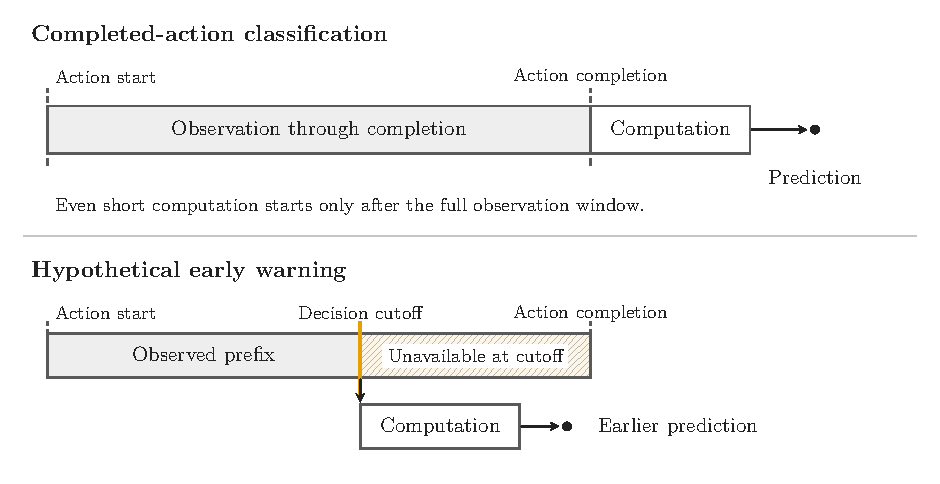
\includegraphics[width=\linewidth]{figures/review_explanatory_20261126/prediction_availability.pdf}
\end{figure}

\section{Multimodal Data in Industrial Applications}

Complementarity is determined by the additional task-relevant information provided by an observation
or representation, rather than by differences in tensor shape or the number of acquisition sources.

Different representations of the same physical quantity can contain complementary information.
Likewise, physically distinct sensors can provide redundant or only very weakly relevant information
for a given prediction target.

The review therefore distinguishes between physical acquisition channels and derived representations
and considers ordinary pairing separately from cases requiring stronger correspondence, such as
cross-modal reconstruction or monitoring of a localised process.

\subsection{Visual and Video Observations}

RGB images, thermal images, process videos and geometric observations all have different acquisition
assumptions. Depth, depth-derived point clouds, and estimated surface normals can all be multiple
views of the same geometric source.

GPAD combines RGB-depth features with point cloud priors \parencite[pp.~4--7]{P024}. This is an
example of integration across representations that do not necessarily require three separate
physical acquisition sources.

RGB-geometry benchmarks describe appearance and shape rather than controller dynamics or motor
current \parencite{Bergmann2022The,Bonfiglioli2023The}.

Physical camera-plus-measurement precedents include thermal imaging with vibration, welding images
with sound, tool images with acoustic emission, and robot video with force/torque and gripper state
\parencite{Huo2022Multisensor,Hua2026Weld,P045,Thoduka2024Handover}.

Their prediction units range from static inspection through to process windows and full trials. In
the tool wear study, the camera is used post-cutting pass, with the preceding acoustic emission
capturing the active cutting \parencite[pp.~19--22]{P045}.

The representation of visual observations also influences the information available. Both pooled
frame features and video Transformers process multiple images, but they differ in how they treat
temporal relationships.

These distinctions between them lead us to explicitly consider visual acquisition, observation
windows, and aggregation within multimodal monitoring architectures.

\subsection{Sensor Time Series and Process Measurements}

Machine measurements can vary enormously in their physical origin and in their semantic meaning. An
accelerometer measures vibration, a pressure sensor measures fluid behaviour, and controller logs
can contain commands, estimates, or tracking errors rather than a direct measure of a physical
quantity.

The harmonic-drive study combines high-frequency vibration with servo information, whereas PGMTKD
transfers pressure-vibration teacher knowledge to a pressure-only student
\parencite{Yang2024Fault,Li2025PGMTKD}.

Both papers address incomplete information, but their sensor availability and deployment reasons
differ.

Representations can also inflate the apparent number of modalities without including any new
measurements. \textcite{Kullu2022A} combine current and vibration using both raw and STFT representations.
\textcite{Wan2024Pipeline} derive statistical 'vibration' features from two acoustic sensors
without acquiring an accelerometer channel at all. \textcite{Wang2025A} combine
source domain features with the decisions from the vibration data.

These studies are useful as architectural comparators, as they examine different information
representations. Their results should, of course, be treated as distinct from comparisons that
incorporate additional physical acquisition sources.

An acquisition inventory and a description of the retained representations are required prior to
attributing any predictive gain to modality diversity.

\subsection{Audio Observations}

Audio can pick up machine/process events that are only very weakly visible. The relationship to
fault state depends heavily on background conditions, mic location, and sync.

MIMII deliberately incorporates factory background recordings at a range of signal-to-noise ratios.
Its fan baseline AUC drops from .94 at $+6$~dB to .70 at $-6$~dB \parencite[Table~3]{Purohit2019MIMII}.

ToyADMOS provides miniature machine recordings and an explicit noise-mixing protocol, making it a
useful reference for acoustic monitoring \parencite{Koizumi2019ToyADMOS}.

In process monitoring, airborne acoustic signals can be paired with either a melt pool camera or a
photodiode. Signal-to-image encoding in the study by \textcite{Li2022A} is an acoustic-optical-signal experiment,
and \textcite{Xie2025Audiovisual} use actual camera images.

DCASE2020 Task2 provides audio-only baselines under an evaluation protocol that differs from that of
later domain shift challenges \parencite{Koizumi2020Description}.

Together, these studies motivate acoustic representations as candidates for industrial multimodal
monitoring. Their utility will depend on the availability of appropriate recordings, well-defined
targets, and correspondence with other observations.

\subsection{Synchronisation, Correspondence, and Modality Availability}

Fusion requires observations that refer to a compatible event, region or time interval. Predicting
one modality from another or combining aligned spatial discrepancy maps requires stronger
correspondence.

RGB-point cloud feature mapping uses registered benchmark geometry. Process monitoring may instead
require time synchronisation and projection onto a common spatial grid
\parencite{Costanzino2024Multimodal,Petrich2021Multimodal}.

In the inspected author manuscript, the digital twin study maps sensor features and prediction
outputs to robot TCP positions. These positions provide spatial registration; they are not among
the 27 listed sensor features \parencite{Chen2023Multisensor}.

Modality availability has several levels. A file can exist without having a usable paired
observation for a given prediction unit. A file can have a successfully paired observation which is
still degraded.

The acoustic-photodiode study explicitly lacks modality registration, which limits claims about
correspondence between its two encoded streams \parencite{Li2022A}.

For camera and machine sensor monitoring, we can have an explicit pairing rule that picks up
unmatched events even if both underlying files are present. Modality completeness should therefore
be assessed on a prediction-unit basis rather than inferred from the presence or absence of the
files.

\section{Representation Learning for Industrial Monitoring}

The choice of representation depends on what an industrial prediction task requires.

The literature reviewed supports both engineered and learned representations. Which is more
appropriate will depend on the level of supervision, the level of preprocessing, the level of
independent sample support, the information required, and the resources available for model fitting.

\subsection{Engineered Features and Conventional Machine Learning}

Engineered summaries impose a constraint on the information that a predictor can use. Measures of
location, spread, amplitude, and trend can describe an operating state without requiring a
high-capacity sequence model to be estimated from a small number of independent observations.

The literature is replete with evidence of compact representations. Hand-crafted local geometry is
competitive in 3D inspection, and a hydraulic CNN paper reports 1.7\% error for its best single
sensor versus 20.5\% error for all seventeen sensors \parencite{Horwitz2023Back,Goodarzi2023Deep}.

These results highlight the necessity for robust conventional references and careful selection of
predictive information.

Industrial vision also offers lightweight alternatives. The weakly supervised inspection network
uses a single camera, internal anomaly-aware features, and a compact CNN. Reported computational
cost is 2.33 million parameters and 5.65~ms per image \parencite[Table~V]{P035}.

The study provides some relevant evidence on representation efficiency, but the anomalous training
labels and modified MVTec supervision differ significantly from normal-only inspection.

Conventional and learned representations should be compared using the same prediction target,
assessment observations, and appropriately fitted preprocessing, rather than ranked solely by model
family.

\subsection{Pretrained Visual Representations}

Pretrained visual representations provide a strong scientific explanation for transferring knowledge
learned from large image collections to industrial applications with far less supervision. The
features they learn may well contain the local appearance, texture, and object configuration
relevant to the downstream prediction task.

PatchCore successfully employs pre-trained, locally aggregated intermediate CNN features together
with a memory of nominal patches for industrial inspection \parencite[Section~3]{Roth2022Towards}.

This provides evidence for investigating transferred spatial representations, though its
nominal-only patch retrieval differs significantly from supervised action classification.

RT-DETR provides another architectural precedent in the form of its multi-scale visual backbone
\parencite[Sections~4.1--4.2]{Zhao2024RTDETR}. Features at several spatial scales would be viable
candidates for the prediction target.

Its published detection accuracy and computational performance pertain to the complete detection
architecture rather than the downstream classification performance of the extracted CNN features.

Asymmetric student-teacher and cross-modal mapping methods also provide further evidence for
task-specific use of the learned visual representations
\parencite{Rudolph2023Asymmetric,Costanzino2024Multimodal}.

Vision-language inspection introduces semantic information as another potential source of
representation value. DSE-AD combines historical and current rail images with normal and abnormal
position prompts and assesses pixel localisation on a further rail domain \parencite{P031}.

Its pair-reference and prompt assumptions differ significantly from those of isolated image
classification.

Together, these studies point to pretrained visual features as plausible candidates, while also
highlighting the need to assess their actual information content, trainable parameters, and
observation horizon in the downstream monitoring task.

\subsection{Temporal and Time-Series Representations}

Temporal representation learning provides an opportunity to retain sequence information that would
otherwise be lost in engineered summaries.

PatchTST addresses this through patch-based time-series representations and shared modelling across
channels \parencite[Sections~3.1--3.2]{Nie2023PatchTST}.

On the Weather dataset at a forecasting horizon of 96, the patch-plus-channel independent model
obtains an MSE of .152, compared with .164 without patching \parencite[Table~7]{Nie2023PatchTST}.

This provides positive evidence for patch-based representation learning in the forecasting setting
under consideration. However, the relevance to industrial classification warrants separate
investigation, as the prediction target, normalisation, supervision, and aggregation differ.

Video representation learning looks at another temporal structure. TimeSformer and Video Swin model
the spatial and temporal relations between video frames \parencite{P034,P013}.

These approaches provide an alternative to simply averaging independently encoded frames. The
industrial CNN-LSTM remaining useful life study also shows the importance of observation length
within its simulated prediction task \parencite{AlDulaimi2019A}.

The literature therefore motivates comparisons that explicitly account for sequence length,
observation windows, temporal ordering, normalisation, pre-training, and fitting budget.

A Temporal Transformer and a compact statistical representation could well be preserving different
aspects of the same sensor stream. Looking at their individual and combined performance helps assess
whether the additional representation contains useful information for the task at hand.

\subsection{Audio Representations}

Acoustic representations include MFCCs, log-mel spectra, wavelet maps, GASF transforms and learned
features.

The Welding Penetration Network uses VMD and GASF; DMAW uses Transformer representations adapted to
the welding observations \parencite{Hua2026Weld,P003}.

These are alternative forms of acoustic representation. An image-shaped acoustic representation is
still one derived from sound rather than being an independently acquired camera stream.

The Audio Spectrogram Transformer is a pretrained candidate for acoustic representation learning
\parencite{P011}. The results on the general audio benchmark are sufficiently promising to warrant
industrial investigation. However, the appropriateness of such representations will depend heavily
on the particular acoustic environment and the specific prediction task.

MIMII and ToyADMOS both go some way to establishing the importance of background composition and
noise environment \parencite{Purohit2019MIMII,Koizumi2019ToyADMOS}.

Together, these studies lead one to consider recording quality, normalisation, and consistent
observation intervals when looking at audio representations.

\subsection{Frozen Representations, Fine-Tuning, and Computational Restrictions}

Freezing an encoder, fitting a small prediction head and then adapting the entire network all
consume different amounts of statistical and computing resources.

Benchmark methods based on pretrained features show that you can get useful representations without
going through the entire original representation-learning process on the industrial dataset
\parencite{Roth2022Towards,Costanzino2024Multimodal}.

The computational cost of pretraining is still part of the representation's provenance even if it's
external to the downstream experiment.

Frozen feature extraction can therefore enable comparisons under a constrained fitting budget.
Fine-tuning provides a very different opportunity in that it allows you to adapt the representations
to the particular target observations. Which of the two is ultimately more effective can only be
determined by empirical comparison, rather than by assuming one approach is in principle better than
the other.

Distillation also makes a further distinction between training and deployment. The PGMTKD multimodal
teachers are used to enrich a pressure-only student. The gated acoustic-vibration study reports a
distilled LightGBM student, though the nature of the teacher features and the timing of the inputs
remain ambiguous \parencite{Li2025PGMTKD,Huang2026Rolling}.

Resource comparisons should therefore account for feature extraction, preprocessing, trainable
components, and any teachers required during inference, rather than just the final prediction model.

These results motivate comparisons of representation and fitting procedures under plausible computing budgets.

\section{Multimodal Fusion Strategies}

Fusion strategies can be broken down according to where the information is fused. Early integration
fuses raw observations or raw features. Intermediate integration fuses the learned representations.
Prediction-level fusion fuses the outputs (e.g., class probability estimates, anomaly scores).
Hybrid architectures use more than one level of integration.

These provide an operational taxonomy for comparing the studies reviewed. Adaptive reweighting
refers to whether the combination varies according to the observation or its context and can
therefore operate at different fusion levels.

Terminology from the source papers is kept where appropriate, and comparisons are based on the
actual location and mechanism of information exchange.

\subsection{Unimodal References and Incremental Modality Value}

The strongest credible single-input predictor provides the reference for measuring the incremental value of fusion.

DMAW fuses the image and
audio Transformer representations to classify the four welding states. The reported accuracy is
96.1\% with fusion, 90.2\% for the image model and 84.4\% for the audio model \parencite[Table~III]{P003}.

This supports a predictive benefit from the assessed multimodal pipeline. The grouping of the
assessment windows by welding run is still not resolved in the evaluation.

In contrast, the weld penetration study reports 100\% clean test accuracy for its image-only,
audio-only, and fused models \parencite[Tables~1--3]{Hua2026Weld}.

The additional modality therefore provides no measurable gain in accuracy under that comparison.

A similar distinction is made in the case of robotic monitoring. The HANDOVER study reports 69.1\%
accuracy for video plus force/torque and 67.9\% when gripper state is added to the I3D-D family
\parencite[Table~III]{Thoduka2024Handover}.

These are five-class outcome accuracies averaged over five training runs. Within that comparison, adding an observation reduced predictive performance.

The tool wear study reports an MAE of 6.6183 for their proposed model, 8.3002 for the visual
ResNet50 and 60.5118 for the acoustic reference. All the other multimodal architectures evaluated
have errors in excess of 45 \parencite[Table~1]{P045}.

The strong visual reference makes the improvement scientifically informative, though the
architectural differences mean you cannot attribute all of it to fusion.

Transferable results on the difficulties of multimodal optimisation and on industrial all-channel
losses underline the need to establish incremental gains against a strong admissible reference
\parencite{Wang2020What,Goodarzi2023Deep}.

Collectively, these studies support investigating the value of conditional fusion, rather than
assuming that including additional modalities will necessarily improve prediction.

\subsection{Feature Concatenation}

Feature concatenation combines the representations with no explicit mechanism for adaptive
allocation and is therefore a key reference point for any more sophisticated form of integration.

Effectiveness depends on feature scale, dimensionality, regularisation, and the quality of the
constituent representations.

M3DM's direct concatenation ablation is worse than its point cloud reference, while the full hybrid
system outperforms both individual inputs \parencite[Table~4]{Wang2023Multimodal}.

MADFlow also provides a further protocol-specific comparison between alignment and concatenation
\parencite{Li2025MADFlow}.

CFA provides transferable evidence from forecasting. For DLinear on the Energy dataset, the first
concatenation gives an MSE of .670, compared with .263 without text and .243 with constrained fusion
\parencite[Table~4]{P023}.

The constrained fusion method also performs worse in a number of the evaluated scenarios, which
again suggests that the benefits of an integration mechanism are highly task-dependent.

Manufacturing fusion can similarly improve one architecture at the expense of the other under the
same broad prediction task \parencite[Table~3]{Li2022A}.

These results establish concatenation as a valid comparator. It should be appropriately normalised
and fitted, rather than implemented as an artificially weak baseline against which more complex
methods are compared.

\subsection{Prediction-Level and Late Fusion}

Prediction-level fusion involves fusing the outputs of modality-specific predictors via techniques
such as averaging, stacking, or evidence aggregation. This is a classification of where the fusion
occurs; the individual predictors could be trained independently or as part of a wider training
regime.

Thermal-vibration diagnosis provides direct evidence of physical camera-sensor prediction-level
fusion. They use separate CNN softmax outputs with weighted Dempster-Shafer aggregation and report a
clean 100\% diagnostic rate, compared with 99.06\% for IRT and 96.32\% for vibration \parencite[Table~VII]{Huo2022Multisensor}.

The weights were fixed, and the sample-level cross-validation did not establish independence between
physical runs.

HANDOVER compares late outputs with intermediate sensor integration in the RGB and optical flow
branches \parencite[Section~IV.A, Figure~3 and Table~III]{Thoduka2024Handover}.

Cross-modal feature mapping and CPIR combine discrepancy maps, which need not be probabilities
\parencite{Costanzino2024Multimodal,Shangguan2025CPIR}.

Some papers also use the term 'late fusion' to describe representation-level integration prior to
classification \parencite{Wang2020What}. That underlines the importance of knowing
what information you are actually fusing.

Stacked generalisation provides a scientific basis for learning a second-stage combination from
cross-validated predictions. Probability outputs contain predictive information beyond the hard
class labels so that a second-stage learner can estimate the joint utility of the outputs
\parencite[Sections~2--3]{Ting1999Issues}.

Ting and Witten fitted a linear least-squares combiner to the class probabilities. A test of such a combination needs predictions for observations held outside the fitting of its component models \parencite[Sections~2--3]{Ting1999Issues}.

\subsection{Gated and Context-Conditioned Fusion}

Adaptive fusion is scientifically justified when the utility of the individual inputs varies from
observation to observation.

Gated Multimodal Units do provide evidence of transferable conditional representation integration.
The architecture fuses visual and textual information and achieves a macro F-score of .541, compared
with .521 for the concatenation baseline in the movie-genre classification task \parencite[Section~3.1, Table~2]{P006}.

The gate in that study operates on learned representations before classification.

Adaptive integration has also been looked at in an industrial context. DMAW achieved 96.1\%
accuracy, compared with 90.5\% for summation and 92.6\% for its gate comparator \parencite[Table~V]{P003}.

TC-MAF provides another approach whereby the auxiliary RGB evidence is bounded around a multimodal
anchor using normal training dispersion and local disagreement \parencite[Section~3.3, Equations~2--4]{P026}.

These architectures illustrate various approaches to controlling information contribution.

An important evaluation dimension is what governs the allocation. GCCF-AD is described as dynamic
fusion, but the formulation they report is a learned scalar with no explicit sample-quality input
\parencite[p.~149226, Equation~8]{P038}.

PGMTKD uses training losses to assign teacher contributions, and task loss balancing focuses on
optimisation rather than any direct measure of input quality at deployment
\parencite{Li2025PGMTKD,P045}.

GAF-Net uses progressive feature feedback, and trustworthy fusion employs evidence-based aggregation
\parencite{Huang2026Rolling,Ying2025Trustworthy}.

The scientific distinction is what contributions can vary, what information determines that
variation, and whether that variation improves predictive performance relative to a fixed
combination.

Process-conditioned weighting provides an additional way to incorporate pertinent context, without
requiring explicit physical law-constrained modelling.

\subsection{Comparability and Fairness of Fusion Evaluations}

A shared dataset name does not in itself constitute a matched experimental comparison.

Cohort construction, supervision, observation windows, pretraining, feature dimensionality,
augmentation, and selection exposure could all contribute to differences between architectures.

The tool wear study alters the architectural components as part of the fusion, and the incomplete
federated imagery study alters the client data access as well as the combining mechanism
\parencite{P045,P051}.

These are comparative assessments of fitted pipelines. Their interpretation differs from an
experiment intended to isolate attention, modality contribution, or quality conditioning.

Comparisons using the same evidence sources can support a narrower attribution. TC-MAF retains the
same evidence sources, comparing bounded fusion against static averaging, weighted scores, rank
fusion, and a learned gate \parencite[Table~3]{P026}.

On the flip side, the disagreement-aware study uses a locally released code baseline that performs
worse than the published M3DM result \parencite[Table~4]{P033}.

Distilled predictors can also access training information that is not available to standard unimodal
models \parencite{Li2025PGMTKD}.

These settings remain scientifically valuable, provided that the information and fitting conditions
are clearly specified. Pipeline performance, incremental modality value, and the isolated effect of
a fusion operator represent distinct evaluation questions.

\section{Reliability and Robustness}

The reliability of a multimodal architecture depends on both the prediction setting and the type of
intervention acting on its inputs.

Missing channels, corrupted measurements, asynchronous observations and changes in operating
conditions all represent different reliability issues. The evidence reviewed is therefore grouped by
the particular condition under consideration rather than assigned to a single general robustness
category.

\subsection{Missing Modalities}

Planned single-input deployment differs from an unannounced loss of an input in a model that
normally expects complete observations.

In the initial appraisal, four of the 37 works examined planned missing-input inference and one examined simulated dropout (five of 37, or 13.5\%, Table~\ref{tab:literature-matrix}). This count combines two missing-input codes. The expanded summary instead records eleven direct tests of missing inputs at inference among 94 appraisals (Figure~\ref{fig:review-depth}); it classifies the depth of evidence rather than the type of absence. The denominators and coding questions therefore differ, and the retained records do not provide a per-work crosswalk between them.

PGMTKD's pressure-only student and incomplete RGB-geometry methods do provide evidence for reduced
input inference. ModDrop and the missing-modality Transformers add further transferable mechanisms
and counterexamples \parencite{Li2025PGMTKD,Sui2026Incomplete,P005,P016}.

The effectiveness of these mechanisms will, of course, depend on the training conditions and the
specific missing-input patterns they have been assessed on.

TC-MAF explicitly evaluates unavailable 3D input. I-AUROC drops from .9788 to .9330 and P-AUPRO from
.9901 to .9586 \parencite[Table~3]{P026}.

This provides a quantified example of performance under a given missing modality condition.

Federated substation monitoring varies the proportion of incomplete clients to 80\% \parencite[Figure~8]{P051}.

Its training and client-availability setting differs from an arbitrary inference-time camera
failure.

ZSG-IAD reports input subset comparisons without fully defining the shared checkpoint and training
exposure \parencite{P025}. Missing training images in the hot rolling regime constitute another
availability regime \parencite{Ma2025A}.

These studies collectively indicate the need to explicitly specify available modalities during both
training and inference (i.e., availability masks), the policy for replacement or fallback, and the
system's response when all required inputs are absent.

\subsection{Noise and Partial Degradation}

Physical monitoring studies do provide evidence of a number of controlled degradation mechanisms.
Thermal-vibration diagnosis examines Gaussian noise and vibration bias/stuck faults, while welding
penetration recognition examines artificial interference. Acoustic-thermal and acoustic-vibration
studies look at other noise settings
\parencite{Huo2022Multisensor,Hua2026Weld,Ying2025Trustworthy,Huang2026Rolling}.

These interventions vary in the observations affected, the degree of corruption and the extent to
which the model is exposed to degradation.

At $-2$~dB, noisy IR thermography gives 95.26\%, which jumps to 97.6\% when combined with fault-free
vibration. Noisy vibration alone gives 36.86\%, jumping to 94.2\% when combined with fault-free IR
thermography \parencite[Table~VIII]{Huo2022Multisensor}.

The comparison shows the value of a fault-free companion modality when another observation is
synthetically corrupted.

The welding penetration study reports a fused accuracy of 93.33\% under its interference condition
\parencite[Table~3]{Hua2026Weld}.

The corresponding corrupted unimodal comparisons are required in order to assess the incremental
benefit of fusion in the interference condition. The reported intervention also leaves some
uncertainty about the corruption operator, magnitude, and exposure matching.

Synthetic signal-to-noise interventions provide some controlled experimental evidence, but the
conclusions are specific to the observations affected and the severities tested. Natural
simultaneous degradation and ordinary defective objects are quite different phenomena.

These distinctions lead directly to a comparison of predictions from degraded input against those
from static fusion and single-input predictors under the same reliability condition.

\subsection{Temporal Misalignment and Distribution Shift}

Temporal misalignment and distribution shift both affect multimodal prediction, albeit in different
ways.

A clock offset can break correspondence between observations, whereas a distribution shift can
change the conditions under which the learned representation or predictor is evaluated.

Registration studies have established the importance of alignment in multimodal monitoring.
OmniFuser's repeated within-pass images provide a way to construct paired observations rather than
directly test a synchronisation failure \parencite{Petrich2021Multimodal,Chen2023Multisensor,P021}.

The literature also contains examples of evaluation under changed acquisition conditions. HANDOVER
trains on one robot and evaluates on a different robot \parencite[Table~V]{Thoduka2024Handover}, and there's a rail localisation study that
evaluates a Subway-trained model on high-speed rail
\parencite[Table~III]{P031}.

Target-adaptive methods, target-validated condition studies and independent build experiments are
all different forms of access to the assessment domain
\parencite{Wang2025A,Chu2024A,Huang2026Rolling,Bevans2023Heterogeneous}.

Rebuilding normal memories on Eyecandies using fixed fusion hyperparameters is evidence of recipe
transfer, rather than deploying an unaltered model to an untouched target installation
\parencite{P026,P033}.

Architecture reuse, representation transfer, temporal offset tolerance, and unchanged-model generalisation each require distinct evaluation protocols.

\subsection{Quality-Aware and Uncertainty-Aware Fusion}

Quality-aware fusion is driven by the idea that the predictive utility of an input may vary with its
quality. Signal quality, model confidence, calibrated probability and evidence consistency are all
distinct concepts.

QMF furnishes a theoretical basis for studying sample-dependent weighting via generalisation upper
bounds under stated relationships between uncertainty and loss, assuming a common training and test
distribution \parencite[Sections~3.1--3.2]{Zhang2023QMF}.

The transferable UDML experiments train on controlled Gaussian corruption intensities and recognise
that sample difficulty can be confused with modality corruption \parencite[pp.~4--5, 9]{P022}.

These results lead us to ask whether the quality information we have available helps us identify
when a particular observation is no longer useful.

QMF reports an NYU scene classification accuracy of 70.09\% on clean inputs, compared to 70.30\% for
concatenation. At corruption intensity ten, it reports 55.60\% compared to 51.99\% for late fusion
\parencite[Table~1]{Zhang2023QMF}.

These non-industrial RGB-depth comparisons do show a regime-specific advantage under corruption. The
clean and corrupted comparisons quoted use different reference methods, so they should not be read
as a clean-versus-corrupted trade-off against the same reference method.

The effect of the adaptation mechanisms also differs across prediction endpoints. The disagreement
add-on increases the local MVTec image AUROC from .779 to .800 and, at the same time, reduces the
Eyecandies image AUROC from .810 to .794, even though the pixel metrics have improved \parencite[Tables~4--5]{P033}.

TC-MAF uses normal-training dispersion and local disagreement to control the contribution of
auxiliary evidence \parencite{P026}.

Collectively, these findings establish a scientific basis for reducing reliance on a stream when the
observable context is expected to indicate errors. They also underscore the need to assess the
relationship between available quality indicators and actual predictive reliability.

QMF's theoretical justification does not validate the use of arbitrary quality proxies, and clean
calibration can actually degrade after a distribution shift \parencite{Zhang2023QMF,P008}.

For quality-conditioned weighting, the relevant comparison is with a static model given the same training exposure to corruption. Performance on clean observations also matters.

\subsection{Modality Dropout, Augmentation, and Fallback Mechanisms}

Different robustness mechanisms deal with different aspects of input availability.

Training-time modality dropout exposes the model to certain absence patterns. Imputation produces
substitute observations, and deterministic fallbacks route the prediction to an available unimodal
component.

These approaches can generate similar outputs under certain conditions without relying on the same
learned recovery mechanism.

The fuzzy-regularisation study introduces failures via partial corruption and by replacing the
entire input with a constant or noise. The evaluation is of Gazebo pose regression using random
sample splits of overlapping windows \parencite[Sections~III.A and IV.A--IV.B]{Altinses2023Fuzzy}.

The investigation provides evidence for controlled input regularisation, with independent physical
deployment outage performance remaining unaddressed.

OmniFuser describes dropout and masking without any quantified outage table \parencite[p.~10]{P021}.

Generated replacement observations can also have a negative impact on performance. Replacing the
clean depth with CycleGAN output worsens the synthetic robot benchmark's MSE (from $2.1745 \times
10^{-3}$ to $13.472 \times 10^{-3}$) \parencite[Table~7]{Altinses2025Performance}.

These results motivate individual evaluation of learned recovery, training exposure, and explicit
fallback policies. Static controls, with equivalent degradation exposure and predictions from the
surviving input, provide a useful baseline for assessing adaptive robustness.

\section{Evaluation Beyond Accuracy}

The practical value of a monitoring architecture will depend entirely on how its predictions are
evaluated, chosen, and interpreted.

Accuracy in prediction can be affected by class distribution, assessment grouping and decision
thresholds. A single aggregate score therefore only provides one facet of the evidence needed to
assess the performance of a multimodal industrial monitoring system.

The evaluation questions concern assessment independence, discrimination, calibration, uncertainty, interpretability, computational viability and reproducibility.

\subsection{Grouped Evaluation and Leakage Prevention}

The independent assessment unit may be a weld, a tool, a participant, a recording, a machine or a
build.

Randomly partitioned observations can end up with shared acquisition contextual information or raw
samples. The fuzzy-regularisation study forms 20-step windows with a stride of one and reports a random
division of the samples \parencite[Sections~IV.A--IV.B]{Altinses2023Fuzzy}.

Its assessment therefore doesn't establish performance on unseen trajectories.

Weld run grouping is still unresolved in the closest welding studies \parencite{P003,Hua2026Weld}. These
examples do show a potential dependence between the observations but do not establish any particular
level of leakage.

The HANDOVER authors report an explicit participant-disjoint official split \parencite{Thoduka2024Handover}.

Normalisation, feature selection and model parameter optimisation all require an appropriate split
between model development and model assessment \parencite{P004,P017}.

Out-of-fold stacking provides a mechanism for constructing second-stage prediction inputs without
any in-sample predictions. Its validity is of course also dependent on the way in which the
underlying fitting, selection and calibration folds are constructed.

Repeatedly selecting follow-up experiments after looking at the assessment results introduces
further selection bias, even if the individual model fits would have ruled out their outer test
labels.

These results motivate the development of assessment protocols that account for the physical origin
and dependence of observations throughout the modelling process.

\subsection{Discrimination, Calibration, and Decision Thresholds}

Ranking, probability quality and thresholded decisions are three different aspects of a predictor.

AUROC measures discrimination across thresholds rather than performance at a single operational
false alarm rate or the quality of the predicted probabilities.

MVTec AD shows that useful ranking can exist alongside fairly poor thresholded localisation. The
strict FPR metrics highlight a different aspect of detection performance
\parencite{Bergmann2019MVTec,Costanzino2024Multimodal,Cheng2025Multimodal}.

The rail vision-language study reports pixel-level metrics and optimal threshold F1 score \parencite[Section~IV.B.2]{P031}. These metrics address a completely different evaluation problem than image-level alarm
accuracy at a threshold chosen from the training or validation set.

In manufacturing, \textcite{Petrich2021Multimodal} report an accuracy of .9921 and a precision of .2487 on an
imbalanced layer, which is a clear example of the impact of class distribution and threshold
selection.

Validation-fitted calibration can improve in-distribution probability quality, while dataset shift
can damage confidence estimates \parencite{Guo2017Calibration,P008}.

Proper scoring rules (negative log-likelihood, Brier score, etc.) provide a basis for assessing
probability forecasts \parencite{P055}. Their interpretation differs from that of discrimination or
thresholded classification.

A generated confidence field or evidence mass cannot replace probability evaluation. Metrics should
align with the prediction target and class distribution, and operational thresholds should be
selected using admissible training or validation observations.

\subsection{Uncertainty and Statistical Comparisons}

Seed variation, acquisition group sampling and model selection uncertainty are all different sources
of variation.

HANDOVER's reported standard deviations are for five training runs on a fixed test set, whereas a
group bootstrap of saved predictions samples assessment units conditional on the fitted models
\parencite{Thoduka2024Handover}.

These approaches capture different facets of uncertainty and do not necessarily encompass all the
variation expected from retraining or deployment in a different domain.

Cross-validation folds share training observations. Under the assumptions stated, the classic
variance result shows that no universally unbiased estimator of cross-validation variance exists;
ignoring covariance can substantially underestimate uncertainty \parencite[pp.~1096--1098, 1102--1104]{Bengio2004CVVariance}. Conditional uncertainty intervals can still be useful when the
estimand and dependence assumptions are stated explicitly.

Small fusion effects, ambiguous repetition counts and conflicting descriptions of significance all
warrant the same level of caution \parencite{Gu2024Improved,Xu2025ModalityResilient}.

Paired performance differences on common assessment observations provide a much more direct
comparison than unrelated score intervals. An interval which contains zero doesn't demonstrate
equivalence, and a positive point estimate doesn't establish practical importance without an
appropriate criterion.

\subsection{Interpretability and Its Limits}

Prediction scores, coefficients, gate traces and spatial maps can all tell you something regarding
how the model is behaving.

The attention debate has both counterexamples to faithful explanation and evidence that the learned
attention weights do, in fact, contain useful information. This leads to the conclusion that
interpretability should be evaluated on a task-specific basis rather than drawing general
conclusions from the terminology of the architecture itself \parencite{P036}.

ZSG-IAD measures schema validity, language consistency and coarse-to-final-mask overlap
\parencite{P025}. These provide evidence of various forms of self-consistency.

Their interpretation differs from both independent physical defect causation and calibrated
confidence.

HANDOVER leaves the use of human action prediction as a means of explanation as a future area of
research \parencite{Thoduka2024Handover}.

Describing which signals a model used leaves two further questions open: whether they explain the physical cause and whether the explanation helps an operator make a decision.

Process context should be distinguished from the explicit physical equation constraints \parencite[e.g.,
PGMTKD's pressure model;][]{Li2025PGMTKD}.

\subsection{Modularity, Reproducibility, and Computational Cost}

Modular architectures enable the replacement and comparison of individual representations
and prediction components. Their value for scientific investigation comes from the fact that you
can identify which component is different between conditions.

Modularity does not establish predictive robustness or an advantage over a matched end-to-end
architecture.

An identified version, accessible source code, executable processing and independently reproduced
results all provide various levels of reproducibility assurance \parencite{P009}.

The difference between local and published M3DM results remains unresolved. It motivates checks of
dependencies, valid point filtering, checkpoints, and scoring conventions \parencite{P033}.

Computational comparisons of course also require a common measurement boundary. The CPIR paper
reports lower FPS than CFM, which is a clear performance vs speed trade-off
\parencite{Shangguan2025CPIR}.

The reported 5.65~ms for the lightweight image network doesn't include the independent sensor branch
or acquisition delay \parencite[Table~V]{P035}.

TimeSformer's compute requirements depend on the ImageNet pretraining and the workload it is
evaluated on \parencite{P034}.

Hardware, batch size, caching, synchronisation and the processing stages included all determine
which computational measurements can be compared.

These results indicate the necessity for explicit resource accounting and reproducibility
documentation. Prospective deployment and operator usability remain open questions for validating a
successful offline forward pass.

\section{Critical Synthesis and Research Gap}

The reviewed literature shows that multimodal observations and learned representations can benefit
industrial and robotic monitoring. Their value, however, depends on the prediction task, the
information each representation contains, and the conditions under which the integration method is
evaluated.

The previous sections have identified four related scientific questions: which representations are
appropriate for a given target, whether combining their predictions is valuable, whether that value
is maintained as observation quality degrades, and how the experimental assessments should be
conducted.

\subsection{Findings Supported Across the Reviewed Studies}

There are tangible observations that can be used to improve the performance of a task-specific
monitoring pipeline. DMAW, thermal-vibration diagnosis, HANDOVER and tool wear prediction are all
good examples under their respective assessment protocols
\parencite{P003,Huo2022Multisensor,Thoduka2024Handover,P045}.

Controlled evidence integration can also improve RGB--geometry inspection under intact-input
conditions. TC-MAF separately reports performance when the 3D input is unavailable \parencite{P026}.

The literature therefore establishes that useful industrial multimodal fusion mechanisms and
approaches to dealing with incomplete observations do in fact exist.

Representation learning offers a number of scientifically sound options for extracting information
relevant to the task. Pretrained convolutional features, patch-based temporal representations, and
hand-crafted features are all candidates with some supporting evidence under certain learning and
evaluation regimes \parencite{Roth2022Towards,Nie2023PatchTST,Horwitz2023Back}.

Their suitability for another industrial prediction target will, of course, depend on several
factors, including the observations, the supervision, the aggregation, and the compute resources
involved.

Static and learned fusion mechanisms both offer different avenues for exploiting complementary
information. Stacked generalisation motivates learning combinations of the outputs of individual
predictors. In contrast, gated representation learning and quality-aware fusion justify
context-dependent allocation \parencite{Ting1999Issues,P006,Zhang2023QMF}.

A further well-established distinction concerns input reliability. Planned single-input deployment,
complete inference-time absence, controlled corruption, and target domain adaptation all address
different issues \parencite{Li2025PGMTKD,Altinses2023Fuzzy,P051}.

The consistent finding across the reviewed studies is a conditional benefit under specific tasks and
evaluation regimes, rather than universal superiority of any single representation or fusion
architecture.

Figure~\ref{fig:review-depth} distinguishes a recorded direct test from the use or discussion of a
topic. In this summary, 46 of 94 appraisals record a direct test of adding an input, 21 of
corrupted inputs at test, and eleven of missing inputs at inference; these count the
questions tested, not findings of a benefit.
% The aggregate counts agree with figures/review_figure_table.tex and the 94-work
% corpus register. A per-work crosswalk for the direct-test coding was not retained
% in the inspected appraisal files; this check did not independently recode them.
Training strategy illustrates this distinction: 60 of the 94 appraisals described or used the
training strategy without a recorded direct test, while 28 (29.8\%) recorded a direct test. These
counts describe the depth documented in the appraisals; low frequency alone does not establish
research priority.

\ReviewDepthFigure

\subsection{Unresolved Questions and Research Gap}

The evidence reviewed also contains significant negative and, indeed, conflicting findings.

The same clean-test accuracy is observed for the unimodal and fused welding models. HANDOVER
performance drops when the gripper state is added. Some alternative multimodal tool-wear models
perform worse than the visual reference, although the proposed model improves on it. The Eyecandies
image scores also go down. All of this calls into question the notion of an unqualified fusion
benefit \parencite{Hua2026Weld,Thoduka2024Handover,P045,P033}.

Category-specific geometry losses, poor hydraulic channel combinations, and the difficulties of
multimodal optimisation all reinforce this conclusion
\parencite{Horwitz2023Back,Bonfiglioli2023The,Goodarzi2023Deep,Wang2020What}.

Several mechanisms could account for these results: redundancy, inappropriate representations,
optimisation difficulties, noise, supervision and limited independent sample support. The studies do
not point to a single underlying explanation.

An important unresolved issue is the distinction between a representation's standalone strength and
its complementary predictive value. A representation that is weak in isolation may still provide
information useful for another predictor. Conversely, a strong additional representation does not
guarantee that a fusion mechanism can effectively utilise that information.

Reliability introduces a related source of uncertainty. Adaptive weighting is justified when the
available context can identify changes in unimodal prediction reliability \parencite{Zhang2023QMF,P022}.
The value of conditioning information, its relationship to branch errors, and its comparison with
exposure-matched static alternatives must be investigated on a task-specific basis.

External evaluation adds another boundary. Re-using a procedure with a new dataset-specific fitting,
re-using the learned representation weights and then evaluating an unaltered predictor in a
different domain are all different experimental questions. You cannot just take the results of one
and treat them as equivalent evidence of generalisation.

\section{Final Summary of the Literature Review}

The 94 appraised works support a conditional benefit from multimodal monitoring. In four-state welding classification, combining image and audio raised accuracy from 90.2\% for the stronger single input to 96.1\%. In weld-penetration classification, both individual inputs and their combination reached 100\% on the clean test set \parencite{P003,Hua2026Weld}. In human--robot handover, adding gripper state to video and force/torque reduced five-class accuracy \parencite{Thoduka2024Handover}. Taken together, these comparisons locate the architectural question more precisely: for a given target and observation window, when does a second input retain complementary information, and when does a learned fusion rule use it more effectively than a strong single predictor or a fixed combination under the same fitting and reliability conditions?

\ReviewFollowupTable

\chapter{Technical Foundations and Possible Models}
\label{ch:foundations}

In the failed insertion shown in Chapter~\ref{ch:reassemble}, the first camera frame carried the same
weight as the last. From that recording, the visual
model took 16 frames and averaged their features into a single description of the
action. Reading the frames in reverse order would have given exactly the same
description. For an insertion, this matters. A change near the point of contact may be
visible in only a few frames, and averaging over the whole action can reduce its
influence.

The robot also recorded force, torque, and movement during the insertion. These
measurements offered a second view of the same event. The main REASSEMBLE experiment
first made a prediction from the camera and another from the sensors. It then tested
whether combining the two helped identify failed actions. The recorded failure label
made that comparison possible, even though the physical cause of this particular failure
was unknown.

PHM raised a different question. There, the aim was to predict a numerical indicator of
gear condition from machine measurements. Photographs taken after a run supplied the
target for the main sensor study. A photograph used to define what a model should
predict has a different role from a camera frame supplied to a model when it makes a
prediction. That distinction affects what can be claimed from the fusion experiments in
Chapters~\ref{ch:phm} and~\ref{ch:reassemble}.

\section{What the models predicted}

In REASSEMBLE, each completed action had one recorded outcome: success or failure. The
16 frames from the insertion therefore belonged to \textbf{one prediction}. Treating
them as 16 separate test cases would count the same outcome 16 times. A recording could
also contain several actions carried out under similar conditions. For this reason, the
evaluation kept actions from the same recording together when separating training and
assessment data.

Failure was the positive outcome in REASSEMBLE, ViFailback, and HANDOVER. In MSM, the
positive outcome was an abnormal cutting interval under the label definition used in
that study. PHM used regression because its target was a number. A low error in PHM
meant that a prediction was close to the indicator derived from the photographs.
Establishing how closely that indicator measured actual tooth damage would require an
independent physical measurement.

HANDOVER supplies supporting unimodal and fixed-average results in
Appendix~\ref{app:handover}. Its missing participant-to-trial mapping prevented the
mandatory participant-safe OOF construction for learned fusion, so the presence of
paired modalities alone did not make a fitted stacker eligible.

For the REASSEMBLE insertion, let \(p_v\) be the failure probability estimated from
video and \(p_s\) the probability estimated from sensors. Both estimates refer to the
same action. Their values can differ because the models receive different measurements
and learn different relationships from the training data.

A classification model produces a score. A sigmoid function turns that score into a
value between zero and one. Whether the value is a good probability estimate is a
separate issue. For example, if a model gives many actions a failure probability close
to 0.8, about eight in ten of those actions should fail if the model is well calibrated
in that range. This chapter distinguishes models that combine probabilities directly
from models that first convert them to \textit{log-odds}, using
\(\ell(p)=\log[p/(1-p)]\). The software clips probabilities near zero and one so this
calculation remains defined.

\section{What the camera contributed}

The REASSEMBLE visual model began with a detector trained to find objects in images.
RT-DETR has a convolutional backbone that extracts image features at several scales. Its
hybrid encoder combines information across those scales. A decoder and detection heads
then use the features to predict object classes and bounding boxes
\parencite{Zhao2024RTDETR}. For the insertion study, the available label described
whether the action succeeded. There was no target box marking the place where it failed.

The main experiment used the ResNet18-vd backbone from the
\texttt{PekingU/rtdetr\_r18vd} checkpoint. Its weights stayed fixed. Each hand-camera
frame used the shared RGB preprocessing specified in
Appendix~\ref{app:implementation}, Section~\ref{sec:rtdetr-preprocessing}.

For each frame, the backbone returned three feature maps. A feature map records how
strongly an image feature responds at different positions. The model took the average
response across each map channel and joined the results. This gave 896 numbers per
frame. Averaging those numbers across the 16 selected frames produced 896 numbers for
the completed action. A separately trained classification head used them to estimate the
probability of failure. The detector’s hybrid encoder, decoder, and bounding-box heads
were bypassed in this experiment.

Two details of the insertion disappear during those averages. The first is the exact
position of a feature in the image. The second is when that feature appeared. For
example, one feature might respond strongly in a frame near contact and weakly in the
other frames. Its average could be the same as a moderate response spread across several
frames. The resulting 896 values would not tell the prediction head which pattern had
occurred.

This limitation led to a specific comparison in Chapter~\ref{ch:reassemble}. The main model averaged
frames across the whole action. A later experiment pooled features from the last four of
the sixteen sampled frames, giving the final part of the movement its own
representation. Both models answered a question about a completed action. Testing an
early warning would require an earlier decision time and would exclude every frame
recorded after it.

Previous studies give reasons to compare these choices. Pretrained convolutional
features have been useful in industrial inspection \parencite{Roth2022Towards}, and the
Vision Transformer study showed that the amount of pretraining data affects the
comparison between convolution and attention \parencite{P010}. Video Swin keeps local
information across both space and time, with a computing cost that depends on the clips
and image crops used \parencite{P013}. TimeSformer reported an advantage for separate
spatial and temporal attention on Kinetics-400 and Something-Something V2
\parencite[Table~1]{P034}. The question for REASSEMBLE was narrower: with the available
recordings and training time, did retaining a selected part of the action help predict
its outcome?

PHM also used a model from the RT-DETR family, but its implementation followed a
different route. The software ran a frozen RT-DETR-L detector and collected three
intermediate feature maps during its prediction process. Pooling these maps produced 768
image features. The software added the time taken to extract them, so the regression
head received \textbf{769 inputs}. Any interpretation of this image experiment must
account for that timing value as well as the photograph.

Keeping an encoder frozen also allowed its features to be saved and reused across
training splits. Later experiments investigated what changed when the visual features
themselves were allowed to adapt. In ViFailback, the study distinguished a generic model
pretrained on COCO, a model previously trained with REASSEMBLE labels, and the completed
stages of training on the target task. These models had different training histories.
Comparing their epoch counts alone would miss differences in batch size, learning rate,
image augmentation, and early stopping. Where the record contains only saved features,
it confirms feature extraction. A claim about classification or fusion also requires a
completed assessment.

\textit{Implementation records: \EvidenceRef{E064}{}, \EvidenceRef{E065}{}, \EvidenceRef{E033}{}.}

\section{What the machine sensors contributed}

During a REASSEMBLE action, the robot recorded 22 channels: three force channels, three
torque channels, two gripper channels, seven joint-effort channels, and seven
joint-velocity channels. A brief change in force and a gradual rise in force can have
the same average. The sensor study therefore compared two ways of reading the same
measurements. One described the action with a small set of statistics. The other learned
from short, overlapping parts of the signal.

For the statistical model, each channel supplied ten values: the mean, standard
deviation, median, minimum, maximum, lower and upper quartiles, range, root-mean-square
amplitude, and slope over action progress. Together, the 22 channels produced
\textbf{220 features per action}. For a force channel, the maximum retained the highest
value in the resampled force channel. The range described the distance between its
lowest and highest values. The slope described whether force generally rose or fell as
the action progressed. None of these values, on its own, identified the moment when the
highest force occurred.

These simple features were a serious comparison for the learned model. They captured
useful properties of the robot’s movement, and their compact size made them a practical
reference with the available training data. Other industrial work has likewise shown
that carefully chosen features can compete with learned representations, including in 3D
anomaly detection \parencite{Horwitz2023Back}.

The second sensor model used PatchTST. To prepare its input, each completed action was
represented by 512 positions from start to finish on each of the 22 channels. Position
256 was therefore near the middle of the action, whether that action lasted a few
seconds or much longer. The spacing was measured in \textbf{action progress}. Two
neighbouring positions did not necessarily represent the same number of milliseconds in
different actions. This matters if the signal is later interpreted in terms of physical
vibration frequencies.

Figure~\ref{fig:sensor-patch-tokens} shows how overlapping sensor patches become tokens.

\begin{figure}[htbp]
\centering
\caption{How overlapping sensor patches become tokens}
\label{fig:sensor-patch-tokens}
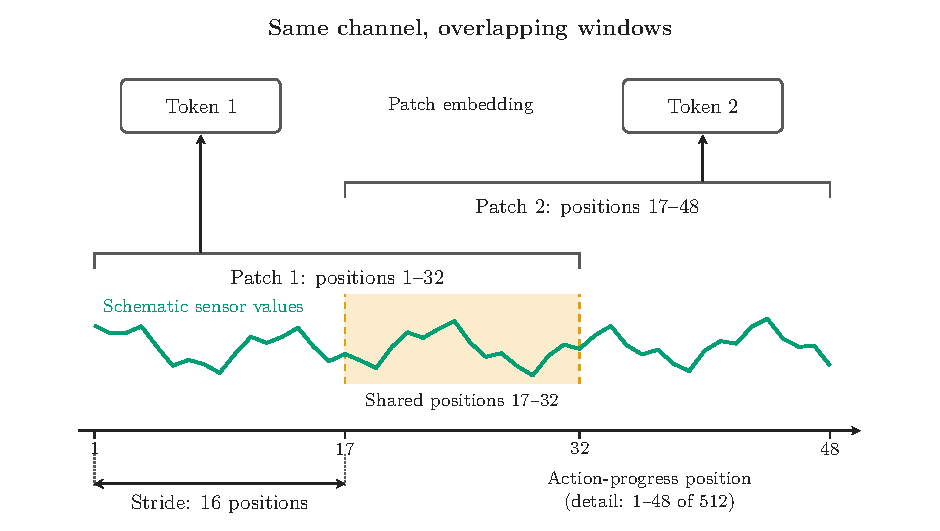
\includegraphics[width=\linewidth]{figures/review_explanatory_20261126/sensor_patch_tokens.pdf}
\displaynote{One schematic REASSEMBLE sensor channel is shown from an action resampled
to 512 positions across 22 channels. Patches 1--32 and 17--48 share positions 17--32;
their starts are 16 positions apart. Each patch becomes a separate Transformer input,
called a \textit{token}.}
\end{figure}

The original PatchTST model processes each channel separately and shares its learned
weights across channels \parencite{Nie2023PatchTST}. This lets it learn from
neighbouring measurements without treating every single measurement as a separate token.
The published model addressed forecasting. In REASSEMBLE, the encoder was trained from
scratch to classify the outcome of a completed action.

The REASSEMBLE model used a patch width of 32, a stride of 16, a hidden width of 32, two
Transformer layers, four attention heads, and a feed-forward width of 64. With no
padding, 512 positions give 31 patches. The number actually processed depends on how the
software handles the end of the sequence. After encoding, the model averaged the patch
features, joined the channel representations, and projected the result to 128 values.
The inputs had already been standardised before entering the model, so internal scaling
was switched off. The software also received a mask identifying observed values. The
effect of a missing value depends on where the model actually applies that mask.

PHM used a separate patch-based model for minute-level sequences of different lengths.
Its default patches were 16 positions wide and started eight positions apart. A patch
was accepted if it contained at least one valid position. The model then used a mask
when pooling the outputs. The length of the sequences in a batch may affect the PHM
patch grid. Its effect on the reported results has not been measured. An optional output
head predicted a sorted profile through positive increments. Once the values were
sorted, the output could describe the profile, but an individual value could no longer
be assigned to a particular tooth.

Other time-series studies help put the comparison in context. TS2Vec found that
replacing its convolutional encoder with a Transformer did not consistently improve
classification \parencite{P012}. MOMENT studied a different training history: its
Transformer learned from several datasets by reconstructing hidden parts of a series
\parencite{P018}. The PatchTST results in this thesis apply to the training data and
budget used here. They leave open what a pretrained time-series encoder might achieve.

\begin{table}[htbp]
\centering
\caption{What reached the PHM and REASSEMBLE prediction heads}
\label{tab:ch3-representations}
\small\singlespacing
\setlength{\tabcolsep}{4pt}
\renewcommand{\arraystretch}{1.15}
\begin{tabularx}{\linewidth}{@{}P{0.26\linewidth}YY@{}}
\toprule
\textbf{Experiment} & \textbf{Input to the prediction head} & \textbf{What the model predicted} \\
\midrule
PHM image model & 768 pooled image features and one extraction-time value & A numerical target \\
PHM temporal model & Features from variable-length sequences of minute-level
measurements & A single value or an optional sorted profile \\
REASSEMBLE visual model & 896 features averaged across 16 hand-camera frames & Success
or failure of the completed action \\
REASSEMBLE statistical sensor model & 220 summary values from 22 channels & The sensor
probability used by the main fusion models \\
REASSEMBLE PatchTST model & 128 learned features from the same 22 channels & A separate
sensor-only prediction in the main comparison \\
\bottomrule
\end{tabularx}
\end{table}

The last two rows in Table~\ref{tab:ch3-representations} are important for interpreting
the experiments. Combining sensor statistics with PatchTST features tests whether two
descriptions of the \textbf{same measurements} work better together. Combining the
statistical sensor prediction with the camera prediction asks a different question:
whether a second physical source adds useful information.

\textit{Implementation records: \EvidenceRef{E031}{}, \EvidenceRef{E065}{}.
Appendix~\ref{app:implementation} gives the model settings.
Appendix~\ref{app:reproducibility} identifies the components used in each experiment.}

\section{What counted as a fair comparison}

In REASSEMBLE, an insertion and a placement did not carry the same risk of failure. The
retained data contained 243 failures in 1,156 insertions and 22 failures in 1,088
placements (Chapter~\ref{ch:reassemble}). A predictor that knew only the action type could therefore
assign a higher failure score to an insertion before using a single frame or force
reading. This is why an action-only reference matters. It measures how much can already
be predicted from the task the robot was asked to perform.

PHM needed a different reference. For a held-out gear run, the constant model returned
the mean target value from the training runs. A sensor model had to improve on that
estimate to show that its readings helped predict the photographic target. The training
mean has a specific mathematical property: among constant predictions, it gives the
smallest squared error on the training data. The median has the corresponding property
for absolute error. The main PHM experiment used the mean.

\begin{table}[htbp]
\centering
\caption{Reference predictions used to judge the models}
\label{tab:ch3-reference-predictors}
\small\singlespacing
\setlength{\tabcolsep}{4pt}
\renewcommand{\arraystretch}{1.15}
\begin{tabularx}{\linewidth}{@{}P{0.28\linewidth}Y@{}}
\toprule
\textbf{Reference} & \textbf{What the comparison asks} \\
\midrule
Training mean & Do PHM measurements predict the gear-condition proxy better than the
same fixed value for every run? \\
Class frequency or action context & How much can already be predicted from the training
failure rate or the type of action? \\
Ridge or logistic regression & What can a regularised model learn from compact features?
Ridge predicts a number. Logistic regression predicts a binary outcome. \\
Single-input neural head & How well does the camera or temporal sensor model perform on
its own on the assessment cases? \\
Histogram gradient boosting & Does the result also hold against a nonlinear sensor
predictor built from decision trees? \\
\bottomrule
\end{tabularx}
\end{table}

The main REASSEMBLE sensor predictor used logistic regression on the 220 statistics. It
learned a coefficient for each feature and an intercept. The study selected its
regularisation setting from 0.1, 1, and 10 within the training partitions. The F2 fusion
model also used logistic regression, but its regularisation setting was fixed at 1. Only
the sensor model selected among those three values.

The visual head and the PatchTST classifier used class-weighted binary cross-entropy.
This allowed failures and successes to carry different weights during fitting. The
original context gates used the unweighted form of the loss. The visual head had 114,945
trainable parameters above the frozen backbone. The PatchTST sensor model had 109,505,
including 90,369 in its projection and classifier. Although the totals were close, the
visual backbone had already been pretrained, whereas the temporal encoder had to learn
from the study data.

ViFailback and MSM also used histogram gradient boosting as a sensor reference. This
method combines decision trees and can learn relationships that a linear model misses.
ViFailback selected a candidate through its validation procedure. The MSM result came
from its own controller-feature protocol. Appendix~\ref{app:implementation} records the
settings for each study.

\section{How the models combined their inputs}

For the REASSEMBLE insertion, the main fusion models received just two numbers from the
prediction branches: the calibrated camera probability \(p_v\) and the calibrated sensor
probability \(p_s\). By this point, the camera branch had already averaged the frames,
and the sensor branch had already reduced the signals to 220 statistics. A fusion model
could change how much it used each prediction. It could not go back to a particular
frame or inspect the force reading at the moment of contact.

Figure~\ref{fig:fusion-interfaces} shows the inputs to the REASSEMBLE stacker and context gates.

\begin{figure}[H]
\centering
\caption{Inputs to the REASSEMBLE stacker and context gates}
\label{fig:fusion-interfaces}
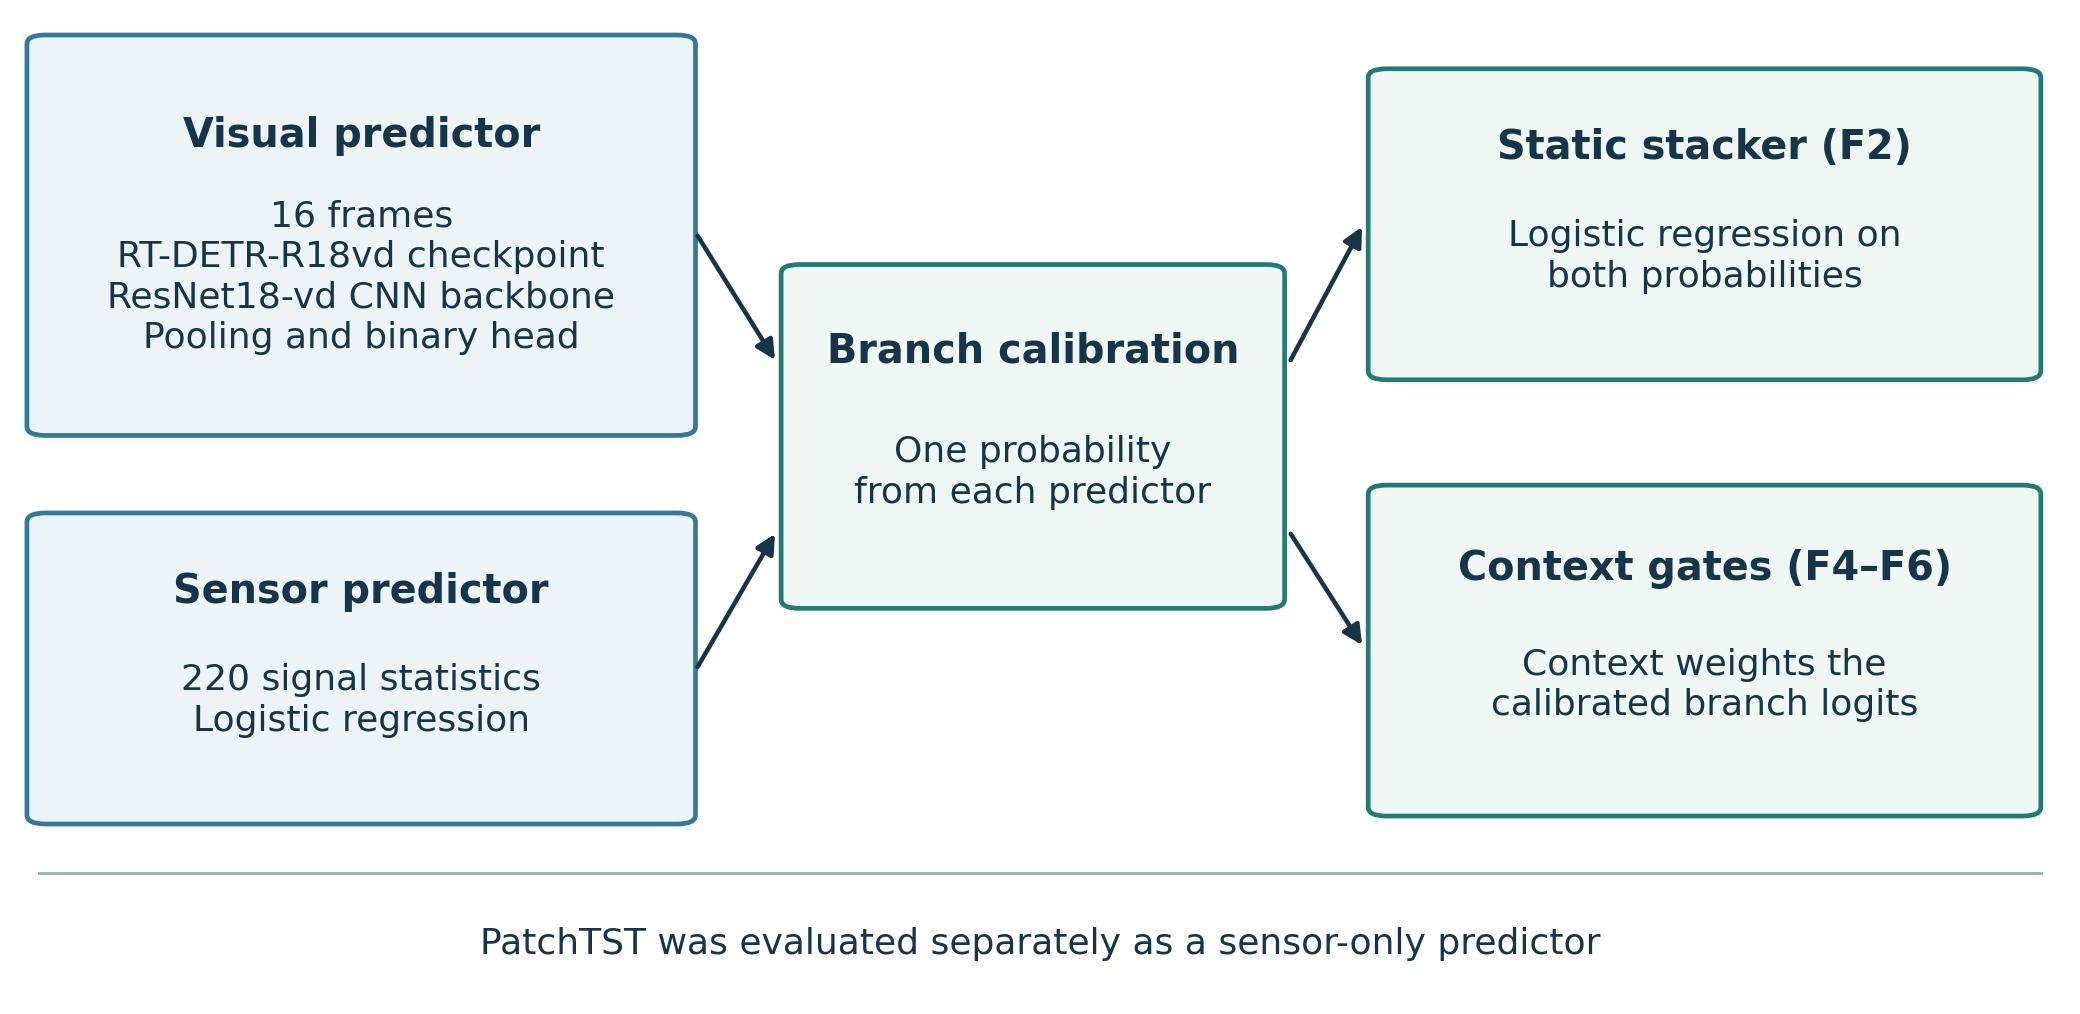
\includegraphics[width=\linewidth]{figures/fusion_interfaces}
\displaynote{The 16 camera frames produced one calibrated prediction. Logistic
regression on the 220 sensor statistics produced the other. F2 used the two
probabilities directly. F4--F6 converted them to log-odds and combined them using
context. PatchTST was evaluated separately as a sensor-only model.}
\end{figure}

\subsection{Feature concatenation in PHM}
\label{sec:ch3-phm-feature-fusion}

PHM combined information at an earlier stage. Its \texttt{fused\_all\_three} model
joined learned features from three groups: process context, root-mean-square vibration
measurements, and condition indicators. One regression head then predicted the target
from the joined features. The software class was called \texttt{LateFusionRegressor},
but the values being joined were features. All three groups came from sensor or process
data. The photographs supplied the target for this comparison. Also, joining features
can increase the number of trainable parameters, so a change in error may reflect both
the extra information and the larger model. \textit{Implementation record:
\EvidenceRef{E004}{Section~12.4}.}

Figure~\ref{fig:workflow-phm-feature-fusion} shows this workflow.

\begin{figure}[H]
\centering
\caption{PHM feature-concatenation workflow}
\label{fig:workflow-phm-feature-fusion}
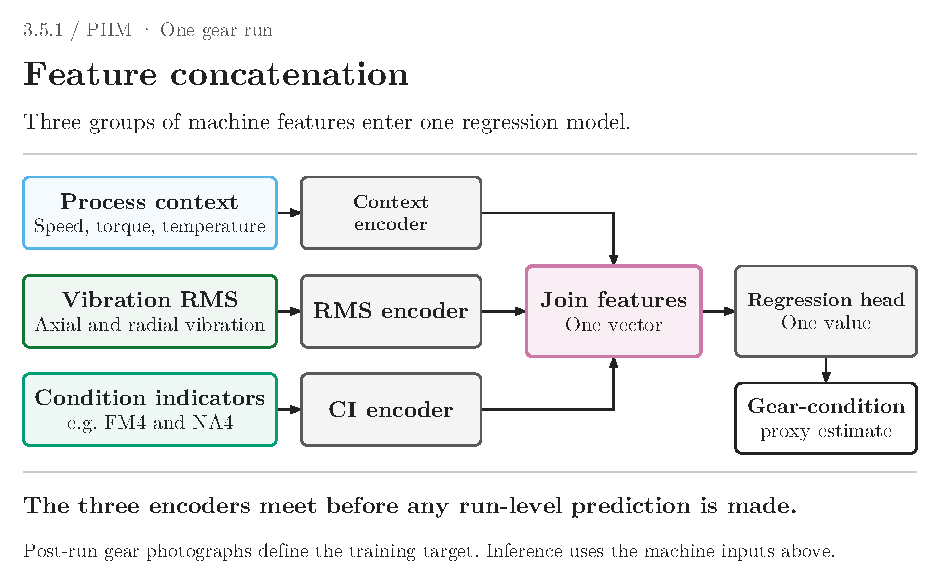
\includegraphics[page=1,width=\linewidth]{figures/fusion_workflows_20261126.pdf}
\displaynote{The inputs are engineered machine features. Post-run photographs define the
condition-proxy target. Here CI denotes condition indicators.}
\end{figure}

\subsection{Equal averaging (F1)}
\label{sec:ch3-equal-averaging}

The simplest REASSEMBLE fusion rule, F1, took the arithmetic mean of \(p_v\) and
\(p_s\). An increase of 0.1 in either branch raised the combined probability by 0.05.
The rule learned no combination weights. The branch models and their calibration still
had to be fitted on training data, and the calibration of their average still needed to
be checked.

Figure~\ref{fig:workflow-equal-averaging} shows this workflow.

\begin{figure}[H]
\centering
\caption{Equal-averaging workflow (F1)}
\label{fig:workflow-equal-averaging}
\includegraphics[page=2,width=\linewidth]{figures/fusion_workflows_20261126.pdf}
\end{figure}

\subsection{Logistic stacking (F2)}
\label{sec:ch3-logistic-stacking}

F2 learned a fixed combination from training predictions. It fitted an intercept \(b\),
a camera coefficient \(\alpha_v\), and a sensor coefficient \(\alpha_s\):

\begin{equation}
p_{\mathrm{F2}}=\operatorname{sigmoid}(b+\alpha_v p_v+\alpha_s p_s).
\label{eq:f2}
\end{equation}

The two coefficients can have different sizes or signs. Within each fitted model, the
same coefficients apply to every action. Their values describe how F2 used the two
branch scores. They cannot identify which physical event caused an insertion to fail.

Figure~\ref{fig:workflow-logistic-stacking} shows this workflow.

\begin{figure}[H]
\centering
\caption{Logistic-stacking workflow (F2)}
\label{fig:workflow-logistic-stacking}
\includegraphics[page=3,width=\linewidth]{figures/fusion_workflows_20261126.pdf}
\displaynote{The coefficients and intercept are fixed within each fitted model. Separate
assessment folds use separately fitted models.}
\end{figure}

Training F2 required care because its inputs were themselves model predictions.
Following the principle of stacked generalisation, the study used predictions for
training actions made by branches that had excluded the corresponding recording during
fitting \parencite{Ting1999Issues}. These \textit{out-of-fold predictions} formed the
prediction bank for the stacker. The outer assessment recordings stayed outside the
fitting process.

One dependence remained inside the training data. F2 reused the prediction bank for its
internal validation. A branch that produced a stacker-training score could therefore
have learned from recordings later used for stacker validation.
Chapter~\ref{ch:methodology} illustrates where this occurred. This detail matters
because using evaluation information to select a model can make its reported performance
look too favourable \parencite{P004}. The check must cover the whole procedure,
including preprocessing, calibration, and the construction of the prediction bank
\parencite{P017}.

\paragraph{Representation concatenation (F3).}
The REASSEMBLE F3 model combined the frozen visual head's 128-dimensional
representation with the 220 sensor statistics. Each input was standardised on the
fitting subset and passed through a separate learned 128-dimensional projection.
The concatenated representation was normalised and supplied to a fitted classifier
that predicted action failure. F3 therefore learned from representations rather than
from the two branch probabilities.\ev{Executed representation-concatenation model}
{\EvidenceRef{E048}{}, \EvidenceRef{E066}{}}

\subsection{Context-based gating (F4--F6)}
\label{sec:ch3-context-gating}

A fixed stacker applies the same rule to an insertion and a placement. The context gates
tested whether the rule should change from one action to the next. F4 received four
action indicators and two input-availability flags. F5 received 36 measures of input
quality and the two flags. F6 received all 42 values. For the recorded insertion, F4
could use the fact that the robot was inserting a part. F5 instead had access to the
measured properties of the inputs.

For an input \(m\), the gate used context \(u\) to produce a score \(q_m(u)\). The flag
\(a_m\) was one when the input was available and zero when it was missing. The gate
calculated a weight \(w_m\) for each available branch and combined the branch log-odds:

\begin{equation}
w_m(u,a)=
\frac{a_m\exp(q_m(u))}
{\sum_j a_j\exp(q_j(u))},
\qquad
p_G=\operatorname{sigmoid}\!\left(\sum_m w_m(u,a)\,\ell(p_m)\right).
\label{eq:gate}
\end{equation}

When both inputs were present, their weights added up to one. The original gates had no
free final intercept or further calibration step. F2, by comparison, learned an
intercept and operated directly on probabilities. A performance difference between F2
and a gate could therefore have several causes. To isolate the value of changing the
weights, the comparison also had to account for the score transformation, the training
loss, and the opportunity for recalibration.

Figure~\ref{fig:workflow-context-gating} shows this workflow.

\begin{figure}[H]
\centering
\caption{Context-based gating workflow (F4--F6)}
\label{fig:workflow-context-gating}
\includegraphics[page=4,width=\linewidth]{figures/fusion_workflows_20261126.pdf}
\end{figure}

Earlier fusion methods made other choices about \textit{where} the inputs could
interact. Gated Multimodal Units combined internal feature representations
\parencite{P006}. Multimodal attention bottlenecks allowed information to pass through
shared intermediate tokens \parencite{Nagrani2021MBT}. The REASSEMBLE gates had a
narrower task: they weighted two action-level predictions.

\subsection{Anchored adjustment and missing-input fallback}
\label{sec:ch3-anchored-adjustment}

A later experiment began with the fitted F2 stacker and asked whether a small adjustment
for each action could improve it. It kept F2’s intercept and branch coefficients. A
second network used context to multiply each coefficient by an adjustment:

\begin{equation}
p_A=\operatorname{sigmoid}\!\left[
b+\sum_m\alpha_m\{1+\tanh(h_m(u))\}p_m
\right].
\label{eq:anchored}
\end{equation}

Here \(h_m(u)\) is the adjustment-network output for branch \(m\). Its final layer
started at zero, so the model initially reproduced F2 exactly. For a finite output, the
multiplier lies between zero and two. The original coefficient keeps its sign. A control
model used a constant adjustment, which made it possible to test whether changing the
adjustment \textit{between actions} added value.

Figure~\ref{fig:workflow-anchored-adjustment} shows this workflow.

\begin{figure}[H]
\centering
\caption{Anchored-adjustment workflow}
\label{fig:workflow-anchored-adjustment}
\includegraphics[page=5,width=\linewidth]{figures/fusion_workflows_20261126.pdf}
\displaynote{Both inputs were available in the clean comparison. Known input loss used
the separate fallback described below.}
\end{figure}

There are theoretical conditions under which adaptive weighting can help
\parencite{Zhang2023QMF}. In practice, a quality measure must contain information about
when a branch prediction becomes less useful. An observed property of a force signal,
the confidence of the sensor model, and the accuracy of that confidence are three
different quantities. Calibration can also become worse when test conditions change
\parencite{P008}. A later quality-interaction experiment therefore compared prediction
heads with matched exposure to altered inputs during training. It was a separate study
from the original gate comparison.

The difference between a damaged signal and a missing signal is particularly clear in
REASSEMBLE. In one controlled test, six force and torque channels were fixed at their
training medians. The sensor input was still present. Its summaries and quality measures
were calculated again from the altered signals, and the fusion model still had to decide
how to use the sensor prediction. In a declared sensor outage, the evaluator already
knew the branch was missing. It returned the camera probability and used the camera
branch’s own decision threshold. If the camera alone was missing, it used the sensor
branch in the same way. If both were missing, it rejected the input.

With a declared outage, methods that return the same surviving prediction necessarily
give the same result for that action. Handling this case shows that the fallback rule
works as specified. Recognising that six \textit{present} channels have stopped carrying
useful information is a harder test. Research on ModDrop, EmbraceNet, and missing-input
Transformers gives further examples of training for incomplete inputs
\parencite{P005,P007,P016}.

\begin{table}[htbp]
\centering
\caption{Where the inputs met in each fusion method}
\label{tab:ch3-fusion-interfaces}
\small\singlespacing
\setlength{\tabcolsep}{4pt}
\renewcommand{\arraystretch}{1.15}
\begin{tabularx}{\linewidth}{@{}P{0.26\linewidth}YY@{}}
\toprule
\textbf{Method} & \textbf{Information available at the point of fusion} & \textbf{What
was learned} \\
\midrule
PHM feature concatenation & Features from three sensor-derived groups & A prediction
head fitted to the joined features \\
REASSEMBLE F1 & Two calibrated probabilities & The combination rule was fixed at equal weights. \\
REASSEMBLE F2 & The same two probabilities & One intercept and two coefficients shared
across actions \\
REASSEMBLE F3 & A 128-dimensional visual representation and 220 sensor statistics &
Separate projections and a classifier fitted to their concatenation \\
REASSEMBLE F4--F6 & Two branch logits, context, and availability flags & Weights that
could change from one action to the next \\
Anchored adjustment & Branch probabilities and context & Changes to the fitted F2
coefficients for each observation \\
\bottomrule
\end{tabularx}
\end{table}

\section{What the experiments can establish}

The main REASSEMBLE comparison used a frozen camera backbone, a statistical sensor
model, and fusion rules that combined their predictions. PatchTST remained a separate
sensor-only comparison on the same sensor measurements in the core study, and its
performance under a limited training budget leaves open what longer
training might achieve. Appendix~\ref{app:implementation} records the configurations,
and Appendix~\ref{app:reproducibility} identifies which prediction paths were actually
run.

The original research question also included sound. An Audio Spectrogram Transformer was
a possible way to represent it \parencite{P011}. Action-level audio prediction requires
reliable alignment between the sound and the labelled action. Chapter~\ref{ch:reassemble}
explains the decision to exclude audio from the predictive experiment. Its value for
these actions remains open.

The recorded insertion illustrates the boundary of the chapter’s claims. The model had
access to the whole action, so it could use visual evidence near the end. The sensor
model had access to the same action through force and movement measurements, but the
summaries it received had already lost much of the order of those measurements. The
fusion experiment could test whether combining those two predictions helped rank failed
actions on held-out recordings. It could not determine the physical cause of that
insertion failure or the earliest time at which the robot could have detected it.

The later experiments changed individual parts of that setup. Pooling the last four
sampled frames changed which frames contributed to the camera prediction. Longer
temporal training changed the opportunity given to the sensor model. Anchored adjustment
changed the fusion rule. The thesis did not run all three changes together. Each result
therefore belongs to the configuration that produced it. Chapter~\ref{ch:methodology}
describes the recording splits, training decisions, and assessment conditions needed to
read those results correctly.

\textit{Implementation records: \EvidenceRef{E112}{}, \EvidenceRef{E114}{}, \EvidenceRef{E110}{}.}

\chapter{Research Design and Shared Methodology}
\label{ch:methodology}

Of the 4,530 completed robot actions in REASSEMBLE, 509 ended in failure. A model that
predicted success every time would therefore be correct on almost 89\% of the actions.
It would also miss every failure. For this study, a more useful question was whether the
model gave higher failure scores to the actions that actually failed. To test what the
camera added, the camera–sensor model and the sensor-only model had to predict the
outcomes of the same actions, with the same recordings held out for assessment.

The PHM gear study needed a different test. There, the model predicted a number derived
from a photograph taken after a gear run. Its error could be measured in percentage
points against that photographic target. The same error could not tell us how closely
the prediction matched physical tooth damage, because the study had no independent
measurement of that damage.

These two cases explain the main design choice in this thesis. Each comparison starts
with the physical event, the target attached to it, and the information available when
the model makes its prediction. The choice of data split and performance measure follows
from those decisions.

\section{Research design and research questions}
\label{sec:ch4-design}
\label{sec:literature-study-gaps}

The welding studies in Chapter~\ref{ch:literature} give different answers about the
value of a second input. Figure~\ref{fig:fusion-research-gap} shows how those
comparisons led to five questions for reading the empirical evidence. The
requirements organize the historical evidence; they do not imply that every
experiment was prospectively designed around this framework.

\begin{figure}[htbp]
  \centering
  \caption{From welding evidence to requirements for testing fusion}
  \label{fig:ch02-synthesis-requirements}
  \label{fig:fusion-research-gap}
  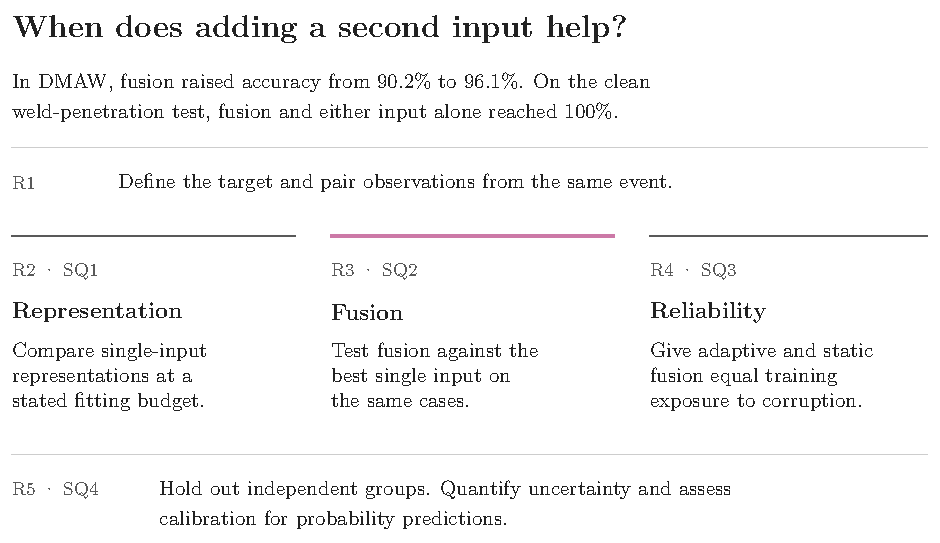
\includegraphics[width=\linewidth]{figures/fusion_research_gap.pdf}
  \displaynote{DMAW reported 96.1\% accuracy for fusion and 90.2\% for
    its strongest single input \parencite{P003}. In weld penetration, both
    single-input models and fusion reached 100\% on the clean test set
    \parencite{Hua2026Weld}. The reported contrasts are within each study.}
\end{figure}

\textbf{R1. What is predicted, and when?} A camera can supply a predictor or a
reference measured after the event. For each study, we identify the physical event,
which observations describe that event, when each was available, and how the target
was obtained. In PHM, post-run photographs supply a proxy for gear condition. In
REASSEMBLE, the camera and sensors are predictors paired with a recorded action
outcome. A readable image or aligned timestamp alone does not establish target
validity or physical correspondence.

\textbf{R2. What does each representation retain (SQ1)?} Published results for
engineered features, pretrained visual features and temporal patches concern
different targets and fitting conditions
\parencite{Horwitz2023Back,Roth2022Towards,Nie2023PatchTST}. We compare individual
branches on the same target and observation window, recording their training
histories and fitting budgets. A branch's standalone score leaves open whether it
contributes information to another predictor.

\textbf{R3. What does fusion add (SQ2)?} The clean welding tie and the loss after
adding gripper state in handover make the strongest single input an essential
comparator \parencite{Hua2026Weld,Thoduka2024Handover}. On the 4,530 eligible
REASSEMBLE actions, we compare camera and sensor predictions, fixed averaging and
fitted combinations with the same recordings held out. The feature-level model F3
projects a 128-dimensional visual representation and 220 sensor statistics to two
128-dimensional vectors and concatenates them. This is distinct from combining
two representations of the sensor stream. Matched opportunities for fitting and
recalibration are needed to isolate the contribution of an additional input.
Chapter~\ref{ch:reassemble} gives the fitting and calibration differences that
limit attribution to the fusion rule alone.

\textbf{R4. Which reliability condition is being tested (SQ3)?} Knowing an input is
absent calls for a different response from receiving a degraded but apparently
available signal \parencite{P026,Zhang2023QMF}. We identify the affected input and
what the model knows about its condition. In the matched REASSEMBLE comparison,
static and adaptive models receive comparable corruption exposure during fitting.
Both are assessed on clean and corrupted cases. Timing changes and transfer to
another domain are separate tests.

\textbf{R5. How dependable is the comparison (SQ4)?} Selection on related
observations can inflate performance estimates \parencite{P004,P017}. The
assessment unit follows the acquisition process, such as a gear experiment,
recording, or manipulation task. Ranking, probability calibration and uncertainty
answer different questions about failure prediction. Fitting and inference costs
also need a stated measurement boundary. Across datasets, we distinguish refitting
a procedure, transferring representation weights and testing an unchanged
predictor. Table~\ref{tab:fusion-study-scope} identifies which comparisons the
available data support; investigating a requirement does not mean that every
condition needed for a strong claim was satisfied.

The published tasks help define the boundaries of the five investigations.
Post-build CT can supply an independent physical reference in manufacturing
\parencite{Petrich2021Multimodal}; PHM instead uses periodic photographs and a
sensor-only deployment specification \parencite{PHM2026Challenge}. Milling studies
of wear and cutting force \parencites[Tables~IV--V]{P021}[Table~1]{P045}
motivate the value of additional
observations, while MSM asks whether video adds information about abnormal cutting
beyond machine telemetry \parencite{Kim2026MSM}. REASSEMBLE's published segmentation
and visual condition-check benchmarks \parencite{Sliwowski2025REASSEMBLE} differ
from the completed-action failure target here. Published handover trials establish
a five-class outcome benchmark \parencite{Thoduka2024Handover}; the supplementary
thesis study instead compares binary failure predictions and their fixed average.
ViFailback's published visual-symbol diagnosis and corrective-action task
\parencite[Tables~2--4]{Zeng2026ViFailback} differs from the binary episode-outcome comparison
here: the latter tests generic and transferred visual features against robot state.
These differences determine the targets and controls; they do not establish a
common cross-dataset leaderboard.

\begin{table}[htbp]
  \centering
  \caption{Inputs and assessment limits of the five thesis studies}
  \label{tab:fusion-study-scope}
  \begingroup
  \singlespacing\small
  \setlength{\tabcolsep}{4pt}
  \renewcommand{\arraystretch}{1.28}
  \begin{tabularx}{\linewidth}{@{}P{.22\linewidth} P{.23\linewidth} Y@{}}
    \toprule
    \textbf{Study} & \textbf{Predictor inputs} & \textbf{Scope and assessment limits}\\
    \midrule
    PHM (Ch.~\ref{ch:phm})
      & Machine sensors
      & R1--R3, R5. Sensor-group comparison against a photographic proxy;
        target validity and modality correspondence limit the claim.
        Camera outages are outside the sensor-only prediction task.\\
    REASSEMBLE (Ch.~\ref{ch:reassemble})
      & Video and machine sensors
      & R1--R5. Principal study of representation and fusion comparisons,
        including adaptive versus static weighting under matched corruption
        exposure on completed actions.\\
    MSM (Ch.~\ref{ch:msm})
      & Video and machine telemetry
      & R1--R5. Primary completed external manufacturing comparison:
        locally fitted branches and fusion, six target/grouping sensitivities,
        and controlled corruption. Assessment covers laboratory cutting intervals.\\
    ViFailback (Ch.~\ref{ch:vifailback})
      & Video features and robot state
      & R1--R3, R5. Task-disjoint assessment and transfer of a specified
        REASSEMBLE-learned visual representation. Target-CNN adaptation was
        assessed on one outer fold; performance under corrupted inputs (R4) was
        unmeasured.\\
    HANDOVER (App.~\ref{app:handover})
      & Video and force--torque measurements
      & R1--R5 with unimodal predictors and fixed averaging. The authors report
        a participant-disjoint test split. Missing participant-to-trial identities
        prevent independent verification and participant-safe OOF fitting of
        learned fusion.\\
    \bottomrule
  \end{tabularx}
  \endgroup
  \displaynote{The R codes indicate which requirements a study investigated.
    Each conclusion applies to that study's target and assessment population.
    The challenge specification and dataset papers document the original
    acquisition and tasks
    \parencite{PHM2026Challenge,Sliwowski2025REASSEMBLE,Kim2026MSM,Zeng2026ViFailback,Thoduka2024Handover}.}
\end{table}

The work was exploratory. For example, the first REASSEMBLE results helped determine
which sensor representation entered the main fusion comparison. Later tests examined
longer training, different camera frames, and changes to the fusion rule. These
experiments answer questions raised by the earlier work. They share part of its history
and, in several cases, its assessment recordings.

Figure~\ref{fig:research-workflow} shows the path from the welding proposal to these studies.

\begin{figure}[htbp]
\centering
\caption{From the welding proposal to the five empirical studies}
\label{fig:research-workflow}
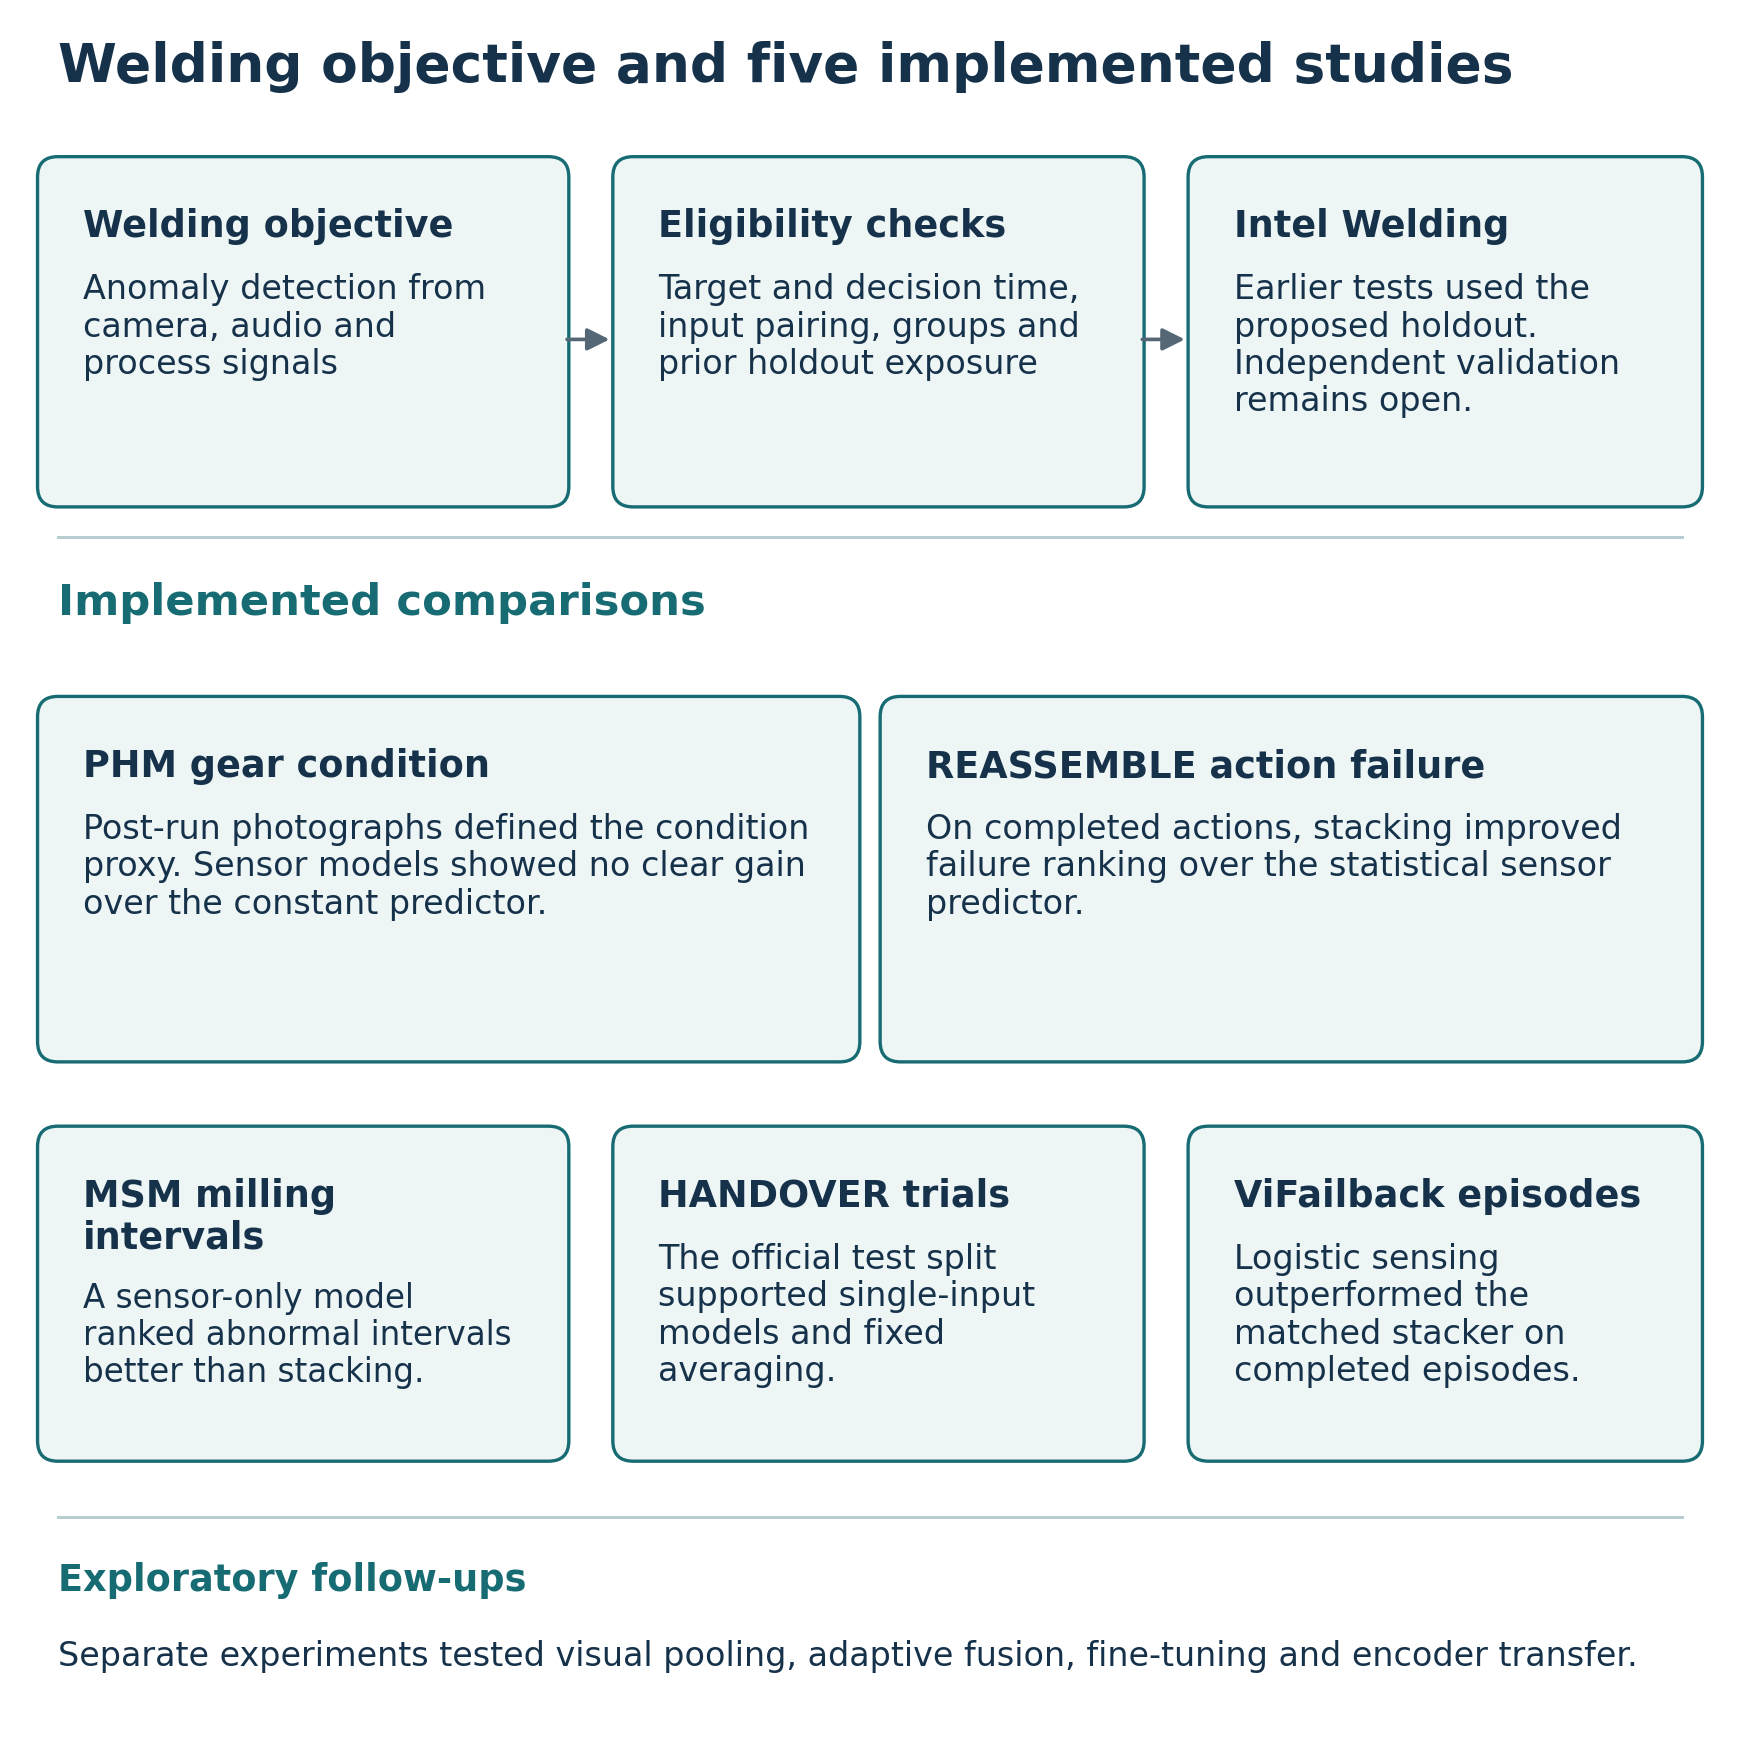
\includegraphics[width=\linewidth]{figures/research_workflow}
\displaynote{The original proposal concerned welding. Checks on the available recordings
limited the planned independent test. PHM, already under way at the renewed welding
audit, provided a study of target construction and sensor prediction, while REASSEMBLE
provided the main comparison of camera–sensor fusion. MSM, ViFailback, and HANDOVER
tested related methods on their own targets. Each result in the figure refers to a
comparison within that study.}
\end{figure}

\section{Dataset selection and order of the studies}
\label{sec:ch4-selection}

A dataset needed more than a video folder and a sensor file. The study needed to
identify the event both files described, the outcome assigned to that event, and the
group to which it belonged. It also needed enough usable observations of the relevant
outcomes to train and assess the proposed models. A dataset could support one part of
the research even when another part remained out of reach.

HANDOVER is one example. The published trial split made it possible to fit individual
predictors and assess their fixed average on the official test trials. Fitting a more
complex combination would also have required suitable groups \emph{inside} the training
data. The available records did not link participants to trials in enough detail to
construct those groups. The study therefore kept the comparison that the data supported.

The welding proposal came first. PHM was already under way when a renewed audit of Intel
Welding identified further limits on the planned test. REASSEMBLE later became the main
setting for comparing visual features, sensor features, and fusion methods. Follow-up
studies addressed questions that emerged during this work. Appendix~\ref{app:chronology}
records the chronology,
including the PADERBORN and REBOOT feasibility investigations.

\section{Why Intel Welding could not provide the planned independent test}
\label{sec:ch4-welding}

The Intel Welding audit checked whether files could be read, how they were timed, which
acquisition session they came from, and whether observations were duplicated. Three
limitations affected the proposed test. The labels described intended welding conditions
rather than independently verified physical defects. Some recordings assigned to assessment had already
been examined during earlier development work on context. In addition, parts of the same
acquisition session appeared in different supplied partitions.

Prior examination did not mean that every test observation had been used to fit a model.
The difficulty was that knowledge of the proposed test material could already have
influenced the design. Session overlap also meant that an assessment sample could share
recording conditions with a development sample. The foundation scripts therefore left
the final test switched off. They provide a record of the data audit. They provide no
final score for the proposed welding fusion model.

The ongoing PHM study permitted investigation of photographic target construction and
sensor prediction. REASSEMBLE provided native completed-action outcomes, paired video
and sensor observations, and recording identities for grouped comparisons of
representations and fusion. An independent answer about
weld quality still requires fresh welding observations, a suitable weld-quality
reference, and a set of welding sessions reserved for the final assessment.

\noindent\textit{Implementation and decision records:}
\EvidenceRef{E017}{inspect\_sample, audit\_split, main}, \EvidenceRef{E016}{},
\EvidenceRef{E118}{}.

\section{Checking the data before fitting a model}
\label{sec:ch4-admission}

Each study used a sample list, called a \emph{manifest}. For each prediction, it
recorded the target, the source files, the observation window, the available inputs, and
the group used for assessment. Where a sample was excluded, the records retained the
reason. Keeping this information made it possible to check later whether two models had
actually been tested on the same cases.

For video, preparation included reading the file, counting usable frames, checking image
dimensions, and finding the part of the recording that covered the event. A frame can
pass all these checks while showing little about why an action failed. Technical checks
establish that an image can enter the model. The recorded outcome and the visible
evidence still need separate consideration.

Sensor preparation included checking channel order, units, timestamps, repeated entries,
and missing values. MSM illustrates why a readable clip is insufficient: choosing the
wrong timing offset pairs a cutting label with a different visual interval.
Chapter~\ref{ch:msm} gives the VMX9 correction and the accepted alignment support.

In ViFailback, duplicate or invalid telemetry records and unreadable video affected
which episodes could enter the comparison. Removing an episode also removes its outcome
from the assessed population. If difficult failures are more likely to have unusable
recordings, the remaining test can become easier. The studies therefore retained counts
before and after exclusion where the records allowed. An excluded observation kept its
original label.

\section{Targets, prediction units, and decision time}
\label{sec:ch4-targets}

For PHM, the principal prediction unit was a gear run. An image-processing rule applied
to post-run photographs measured the area that met the rule’s selection criteria. This
value served as a \emph{proxy}: a quantity available for study when a direct measurement
of the condition of interest was unavailable. The main sensor model tried to predict
this photographic value from machine measurements. Its error describes agreement with
that target. Claims about actual damage, damage to a particular tooth, or remaining
useful life would need their own physical reference.

The robotic studies had recorded outcomes. REASSEMBLE predicted whether a completed
assembly action had succeeded. ViFailback predicted the outcome of a complete
manipulation episode. HANDOVER used a binary outcome for a human–robot trial. In MSM,
the target was abnormal cutting during a labelled milling interval. The main MSM
analysis used its stated mapping of the original labels. Other mappings were examined
separately because changing the meaning of “abnormal” also changes the task.

The end of the observation window matters in each case. A hand-camera frame taken near
the end of an insertion can show part of the outcome. A sensor average over a whole
milling interval includes the final measurements from that interval. Both can be useful
for reviewing a completed event. To test an early warning, the study would need an
earlier decision time, a rule allowing only data already available at that time, and a
measure of how much warning the prediction gave. A short model runtime cannot recover
time already spent waiting for the observation window to finish.

Some inputs also carry information about the experiment itself. In the separate PHM
image-regression experiment, extraction time was one of the inputs alongside the image
features. In REASSEMBLE, action type carried information because insertion and placement
had different failure rates. A gate that changes its weights between these actions may
have learned a difference in task difficulty. To claim that it detected a damaged
sensor, its behaviour must also be tested under a known change in sensor quality.

\section{Keeping development and assessment data separate}
\label{sec:ch4-assessment}

The correct group to hold out depended on how the observations were collected. PHM held
out complete gear experiments. REASSEMBLE kept all actions from one recording together.
ViFailback held out manipulation tasks. MSM examined both experiment-based and
date-based groups. A milling machine or tool could appear on more than one date, so a
test on a held-out date answers a narrower question than a test in a new factory.

HANDOVER used the published official partitions. The dataset publication describes the
test participants as separate from the training participants. The available
participant-to-trial records were insufficient to reconstruct that separation
independently or to make new participant-level folds within training. This is why the
official comparison remained usable while the planned learned stacker had to be left
out.

\subsection{Preprocessing and model selection}

Information can enter a model before the final training step. Consider sensor scaling. A
model may express each reading as a distance from the average training value. If that
average includes the held-out experiment, the test measurements have already influenced
the values given to the model. The same issue applies when filling gaps, selecting
features, tuning a model, adjusting probabilities, or choosing a decision threshold.
These steps need to use the development data allowed for that split \parencite{P017}.
Reusing evaluation results to select a configuration can make its reported performance
look too favourable \parencite{P004}.

The separate PHM four-arm diagnostic illustrates this risk;
Section~\ref{sec:phm-diagnostics} distinguishes its shared normalizer from the
fold-local preprocessing of the principal sensor comparison.

A frozen image encoder presents a different case. If its weights were learned from an
external dataset and its feature extraction uses no target labels or statistics from the
assessment population, the fixed image features can be saved in advance. Later steps
that \emph{learn} from those features still have to respect the training split.

\subsection{Training the REASSEMBLE stacker}

The REASSEMBLE stacker learned from two numbers for each training action: a camera score
and a sensor score. It needed scores like the ones it would receive for an unfamiliar
recording. A score from a branch that had already trained on the same recording could
give the stacker an unrealistically easy example.

The study first set aside the recordings for the outer assessment. Within the remaining
recordings, the camera and sensor models were fitted on some groups and used to predict
actions from other groups. Repeating this process produced a bank of \emph{out-of-fold
predictions}. For each row in the bank, the model that produced the prediction had
excluded that row’s recording. These scores supported training-side calibration, model
selection, and fusion fitting according to the procedure being tested
\parencite{Ting1999Issues}.

One detail limits how independently the stacker itself was validated. Its internal
validation used the same prediction bank. A branch that produced a score for a
stacker-training row could have learned from a recording later used to validate the
stacker. This dependence occurred \textbf{inside the outer training population}. The
outer assessment recordings stayed outside fitting and entered only when the selected
system was scored.

Figure~\ref{fig:stacker-recording-flow} shows the development and assessment paths.

\begin{figure}[H]
\centering
\caption{Recording flow for one REASSEMBLE outer split}
\label{fig:stacker-recording-flow}
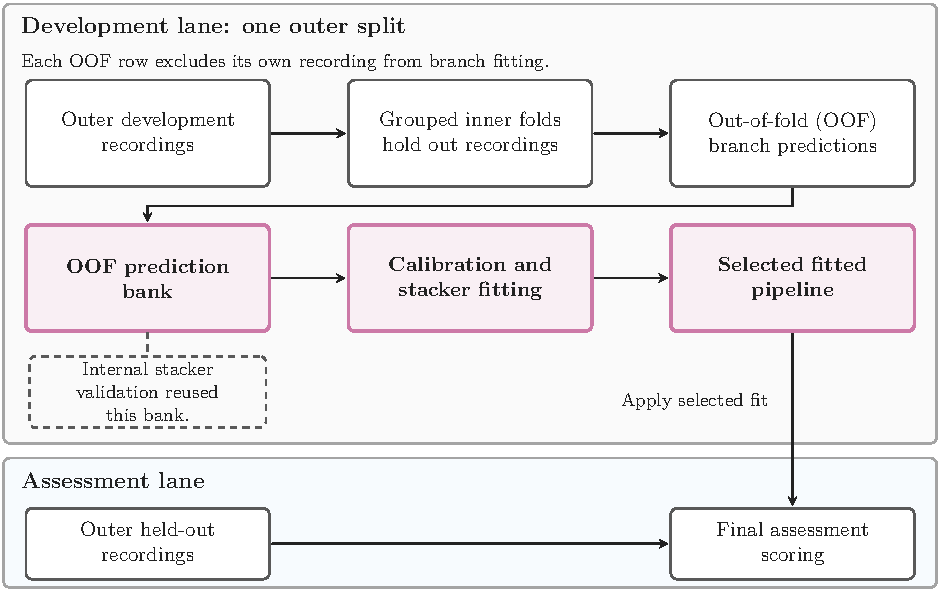
\includegraphics[width=\linewidth]{figures/review_explanatory_20261126/stacker_recording_flow.pdf}
\displaynote{The development lane shows how grouped inner folds supplied the camera and
sensor scores used to fit the stacker. Its internal validation reused that bank. The
assessment lane shows where the held-out recordings first entered the procedure: at
final scoring.}
\end{figure}

\subsection{Checking which actions entered each comparison}

Assessment identities take precedence over shorthand metadata. The REASSEMBLE
follow-ups include a previously examined 753-action subset from 26 recordings;
Section~\ref{sec:reassemble-followups} and Appendix~\ref{app:supplementary-results}
retain the reconciliation and study-specific controls. Sharing assessment cases permits
paired comparisons, but does not make an exploratory follow-up a fresh external test.

\section{Fitting models, adjusting probabilities, and choosing thresholds}
\label{sec:ch4-fitting}

Fitting a model, choosing a model, adjusting its probabilities, and choosing a decision
threshold were separate steps. In REASSEMBLE, for example, training the sensor predictor
determined how its features contributed to its score. Selecting its regularisation
setting determined which fitted version went forward. A calibrator then used
training-side predictions and outcomes to adjust the probabilities. Finally, a threshold
converted each probability into a success or failure decision.

The main REASSEMBLE branch calibrators used sigmoid functions fitted to selected inner
out-of-fold scores. Calibration can improve the meaning of a probability estimate, but
the improvement needs to be checked on assessment data \parencite{Guo2017Calibration}.
The F2 stacker then fitted a logistic combination of the two branch probabilities with
its own intercept. There was no further calibration step after F2. The original context
gates combined branch log-odds using weights that added up to one. They had neither a
free final intercept nor a separate calibrator after the gate.

This difference matters when interpreting the gain from fusion. Suppose a sensor-only
adjustment raises some probabilities while keeping all actions within one fold in the
same order. The ranking within that fold stays the same. A second fold, however, has its
own fitted adjustment. When the two lists are joined, a failure in the second fold can
move above a success in the first. The \textbf{pooled} ranking can therefore change even
though the order within each fold stays fixed.

In the main REASSEMBLE comparison, F2 improved pooled failure ranking over the original
statistical sensor predictor. F2 received both a camera score and an extra fitted step
for combining scores. A sensor-only model given the same opportunity for second-stage
fitting would help separate those effects. The original comparison had no independently
refitted control of that kind. Chapter~\ref{ch:reassemble} examines the saved predictions to see what the
fitted terms contributed. The complete gain cannot be assigned to the camera alone.

For binary decisions, the recorded procedure examined thresholds from 0.01 to 0.99 using
permitted training-side predictions and a stated objective, such as balanced accuracy. A
score at or above the selected threshold counted as positive. This produced a
reproducible decision for the experiment. A factory alarm would need additional
information about the cost of a missed failure, a false alarm, or an unnecessary stop.

\section{Measuring performance and uncertainty}
\label{sec:ch4-metrics}

\subsection{What the reported scores mean}

In PHM, \textbf{mean absolute error} gives the average size of the difference between a
predicted value and the photographic target. \textbf{Root mean squared error} gives
greater weight to larger errors. Both retain the target’s units. The coefficient of
determination, \(R^2\), compares prediction error with the variation in the observed
targets. It can become negative, and it can change sharply when a held-out group
contains little target variation. Tooth-level and run-level errors were therefore
reported at their own levels.

For REASSEMBLE failure classification, \emph{precision} asks how many predicted failures
were actual failures. \emph{Recall} asks how many of the actual failures were found.
Lowering the decision threshold may find more failures while also raising more false
alarms. Specificity measures how often successful cases were correctly recognised.
Balanced accuracy gives equal weight to recall for the two classes, while the F1 score
combines precision and recall for the designated positive class.

The main ranking measure was \textbf{average precision (AP)}. It gives a model credit
for placing positive cases high on its list across different thresholds. The study used
\texttt{average\_precision\_score}, which weights each precision value by the
corresponding increase in recall. Calculating the area under a precision–recall curve by
the trapezoidal rule is a different measure. AUROC also measures ranking, but a
precision–recall analysis is particularly useful when the event of interest is uncommon
\parencite{Saito2015PrecisionRecall}.

The failure rates in REASSEMBLE and ViFailback show why the positive class must be
named. In REASSEMBLE, roughly 11\% of the actions failed. A model that gave every action
the same score would have failure AP of about 0.11. In ViFailback, more than 85\% of the
eligible episodes failed. The same constant-score rule would already have failure AP
above 0.85, despite being unable to distinguish any two episodes. For ViFailback, the
study therefore reported AP for failure, AP for success, and the mean of these two
values. When both classes are present, that mean is 0.5 for a constant-score model. MSM
used abnormal cutting as its positive class. These scores answer different questions
across the three datasets.

Ranking also leaves open whether the probabilities are useful. The \textbf{Brier score}
measures the average squared difference between the predicted probability and the
recorded binary outcome \parencite{P055}. \textbf{Expected calibration error} groups
predictions into probability ranges and compares the scores with the observed outcome
frequencies in those ranges. Its value depends partly on how the ranges are chosen and
how many cases fall in each. A model can rank failures well and still assign
probabilities that are too high. Its probability estimates can also become less reliable
when operating conditions change \parencite{P008}.

\subsection{Combining results and estimating uncertainty}

For its principal comparison, REASSEMBLE brought together the predictions for all
held-out recordings and calculated failure AP once. Calculating AP separately in each
fold and averaging the five results would answer a different question, because cases
from different folds would never be ranked against one another. MSM calculated pooled
abnormal-cutting AP for each training seed and then averaged across seeds. Changing a
seed measures variation from fitting a model again. It does not create another
independently recorded milling interval.

To compare two REASSEMBLE models, the analysis kept their predictions paired. If a
recording was selected for a calculation, both models contributed predictions for the
same actions in that recording. The core comparison repeated this \textbf{2,000 times},
sampling whole recordings with replacement and recalculating the difference in
performance. This is a recording-level \emph{bootstrap}.

A PHM report used 10,000 bootstrap samples drawn at the level of the gear run. The data
still came from only \textbf{20 runs across three gear experiments}. Runs from the same
experiment could share conditions. More bootstrap draws make the numerical estimate more
stable, but they cannot supply more independent gear experiments. The MSM date-based
intervals had a similar limit: only five acquisition dates were available.

The intervals describe variation in the saved predictions under the chosen way of
resampling. They do not cover every change that might occur after retraining the models
or moving to a new installation. The intervals also leave out uncertainty from model
selection and repeated use of the assessment data. Cross-validation folds can also share
training observations, which limits what their spread tells us about uncertainty
\parencite{Bengio2004CVVariance}. Where an interval for a performance difference
included zero, the data left the direction of the advantage unresolved. Showing that two
methods perform closely enough for practical use would require a separate criterion for
how small a difference counts as acceptable.

\section{Testing missing and damaged inputs}
\label{sec:ch4-robustness}

\subsection{What the model knew about the fault}

A missing sensor and a faulty sensor can lead to different decisions. In the REASSEMBLE
absence test, the evaluator knew when a whole branch was unavailable. When the sensor
branch was missing, it returned the camera probability and used the camera branch’s
decision threshold. When only the sensors remained, it used their probability and
threshold. If both inputs were absent, it rejected the case. Fusion methods that
returned the same surviving prediction naturally obtained the same result under this
rule.

A damaged signal presented a harder problem. In one REASSEMBLE test, six force and
torque channels were fixed at their training medians. The sensor branch still received
numbers and could still make a prediction. Its statistics and quality measures had to be
calculated again from the changed signal. Giving the gate quality measures from the
original clean signal would have described a different input from the one the predictor
actually received.

For each controlled disturbance, the important details were what changed, where the
change was applied, how strong it was, and which observations were assessed. Blurring
the camera frames before feature extraction tests a different fault from altering a
saved feature vector. For random noise, the number of noise samples and the
randomisation procedure also affect the result. HANDOVER, for example, included
controlled sensor noise, visual blur, and known loss of an input. ViFailback did not assess performance under missing,
degraded or temporally shifted inputs.

\subsection{Giving competing models the same exposure}

A gate trained with noisy signals has already seen a problem that a model trained only
on clean signals has never faced. If the gate performs better under noise, the training
examples may explain part of the gain. Later REASSEMBLE comparisons therefore gave
static and adaptive models comparable exposure to corruption during fitting. This
addressed one important difference while leaving others, such as model size and
calibration, to be considered. The idea that changing weights can help rests on how well
the available information identifies an unreliable input \parencite{Zhang2023QMF}.

The evaluation considered both the score under damage and the change from the clean
score. A model can lose less from its starting point yet still finish below a stronger
model. When only the sensors were damaged, the intact camera also provided a useful
reference: combining inputs was of limited value if it produced a worse prediction than
using that camera alone. The tests support conclusions about the stated faults and their
severity. Questions about gradual clock drift, several natural faults at once, or
operation in a new factory remain open.

\section{Records, software, and checks on the results}
\label{sec:ch4-reproducibility}

A reported score can be checked at several levels. With saved predictions and outcome
labels, it is possible to check the sample identities and calculate the score again.
Running the fitted model on its inputs also checks whether it produces the same
predictions. Training the model again requires the training data, software, settings,
and selection procedure. Each step examines a different part of the evidence
\parencite{P009}.

The main REASSEMBLE visual branch loaded RT-DETR-R18vd through Hugging Face Transformers
and took its ResNet18-vd convolutional backbone. The same library supplied the PatchTST
sensor encoder, which was trained from scratch \parencite{Wolf2020Transformers}. The
neural models used PyTorch, with AdamW for the relevant fitting steps
\parencite{Paszke2019PyTorch}. Scikit-learn supplied grouped stratified splits, logistic
regression, and evaluation functions \parencite{Pedregosa2011ScikitLearn}. The separate
PHM image model used the Ultralytics RT-DETR-L prediction procedure to collect
intermediate image features \parencite{UltralyticsRTDETR}.

The manuscript’s source record identifies repository commit
\texttt{e32ec43aef69cc58adff0ea91e508308041598c5}. File hashes identify selected source
files and reports, including some material held outside that commit.
Appendix~\ref{app:reproducibility} links the experiments to the available evidence.
Appendix~\ref{app:chronology} records when the work took place. Where an original script
or setting was unavailable, the remaining records limit how much of the run can be
checked independently.

Saved-prediction checks covered the core REASSEMBLE F2 comparison and the available
ViFailback assessments. For REASSEMBLE, they checked sample identities, fold assignments,
branch scores, fitted coefficients and ranking measures. For ViFailback, the retained
analyses checked available episode identities, fit coverage, AP, AUROC, Brier score and
log loss; ECE and threshold summaries remain results from retained reports. Missing
individual prediction or fitting records limit independent reconstruction. These checks
did not repeat neural training or assess newly collected observations.
Table~\ref{tab:vif-status} records the coverage of the ViFailback comparisons.

\noindent\textit{Implementation records:} \EvidenceRef{E062}{}, \EvidenceRef{E063}{},
\EvidenceRef{E065}{}, \EvidenceRef{E044}{}, \EvidenceRef{E031}{}. \textit{Provenance records:} \EvidenceRef{E109}{},
\EvidenceRef{E107}{}, \EvidenceRef{E113}{}, \EvidenceRef{E114}{}, \EvidenceRef{E111}{},
\EvidenceRef{E121}{}.

\section{Computing resources and the scope of the findings}
\label{sec:ch4-boundaries}

The project used HFU server resources. The later ViFailback study recorded a single
NVIDIA Tesla T4 with 16~GiB of device memory. Reusing frozen camera features and compact
sensor statistics made repeated fitting practical. Dataset acquisition and preparation
also required resources: MSM used a bounded download plan for selected laboratory files,
while REASSEMBLE later released approximately 66.9~GiB of derived caches, retaining
source videos, checkpoints, predictions, and recovery metadata. Rebuilding those caches
adds work to a fresh run.

ViFailback logged about 303.8 elapsed hours across two GPU controller processes,
including decoding, validation, and checkpointing; this was neither GPU kernel time nor
total thesis compute. Completing its remaining \texttt{FULL20} matrix was estimated to
require another 43 GPU days on the single T4, with 47 days allowed for variation and
overhead. This forecast of additional work informed the decision to stop further CNN
fitting. It is a resource estimate, not a model-performance result.

The implementation contribution includes acquiring usable observations, maintaining
aligned sample lists, reusing features, and preserving evidence within these limits.
Scientific findings still depend on the completed comparisons. Limited resources do not
establish why a model performed poorly, and an unassessed configuration has no measured
result. Head-only timings exclude frame reading and feature extraction. Timing the
whole model after a completed action still excludes the time spent waiting for that
action to finish. An operational warning claim would need to include acquisition,
synchronisation, preprocessing and inference up to the moment a decision becomes
available. Chapters~\ref{ch:reassemble} and~\ref{ch:vifailback} report study-specific
training coverage and timing boundaries.

The clearest findings come from comparisons in which the competing models saw the
same assessment cases and the difference between them can be stated precisely.
The 753-action REASSEMBLE follow-up can show how a change affected those previously
studied actions. A fresh test of the resulting design would require the target,
decision time, recording groups, models, fault conditions and main performance
measure to be fixed before opening new assessment data.

% Resource provenance (read-only records; HFU server use supplied by the researcher):
% implementations/VIFAILBACK/experiments/matched_cnn_20_100_f2_20261111/18_fit_stop_and_analysis_20261124T1955Z/final_evidence/14_final_research_reports/11_GPU_RUNTIME_AND_STORAGE.md
% E113: implementations/VIFAILBACK/experiments/matched_cnn_20_100_f2_20261111/18_fit_stop_and_analysis_20261124T1955Z/completed_scope_analysis/RESULT_ANALYSIS.md (43-day central estimate; 47-day planning allowance, not a confidence interval).
% implementations/REASSEMBLE/docs/maintenance/REASSEMBLE_CACHE_RETENTION.md
% implementations/MSM/experiments/legacy/PILOT_FINDINGS/05_FULL_LABORATORY_FEASIBILITY/MSM_FULL_LAB_COHORT_AUDIT.md

\chapter{PHM Case Study: Target Construction, Proxy Validity, and Sensor-Group Fusion}
\label{ch:phm}
PHM establishes the target-validity problem that precedes the paired vision--sensor
studies: machine measurements predict a proxy constructed from post-run tooth
photographs. The principal held-out-experiment comparison did not establish lower error
for three-group sensor fusion than for a training-mean constant. Photographs supply
supervision rather than an inference-time image branch in that comparison. Separate
visual diagnostics examine target emulation and appearance agreement without an
independent physical-damage reference.

\section{Study Objective and Relationship to the Research Questions}
The study addresses R1 by separating target validity from the correspondence and
availability of the prediction inputs. For SQ1, the image and sensor experiments assessed whether frozen visual features and
temporal sensor representations could reproduce a specified target. For SQ2, the
principal fusion comparison combined context, root-mean-square (RMS) vibration and
condition indicators, all available at inference. It did not test joint image--sensor
inference. For SQ3, a predictor that already returns nearly constant values can appear
insensitive to corruption, so its clean-input error matters. For SQ4, the training-mean
comparison asks whether measured sensor inputs improved prediction over a rule that
ignores them at inference. It cannot establish whether the photographic target measures
damage. That question requires a physical reference independent of the rule.\ev{PHM
target and deployment inputs}{\EvidenceRef{E019}{}}

\section{Dataset, Acquisition Structure, and Supervision Challenges}
The retained population contains EXP-A runs 1--5, EXP-B runs 1--7 and EXP-F runs 1--8:
twenty nominal run units across three experiments. A run can contain multiple tooth
photographs, camera-sequence views, high-frequency vibration members, low-frequency
context measurements and condition-indicator records \parencite{PHM2026Challenge}.
An image, a minute-level feature
row and a run are consequently different observational units. Repeated views and long
sensor sequences increase the number of stored observations without increasing the
number of independently acquired experiments to the same extent.

Experiment and run identifiers are retained through derived manifests. Tooth identity
and image role define target generation, whereas archive/member identity and measurement
provenance define sensor features. Their correspondence is principally at run level.
This supports joining measurements to a post-run proxy, rather than asserting
hardware-synchronised image/sensor events or prospective image availability. These associations are documented in the manifests and implementation; the raw archive
contents have not been fully rechecked independently.\ev{PHM experiments and acquisition
sources}{\EvidenceRef{E018}{}}

\subsection{Supervision and Dependence Limits}
The target depends on acquisition geometry, illumination, texture and image-processing
choices as well as possible surface damage. In EXP-A and EXP-B, tooth indices 1--4 and
5--28 had different image-role coverage. Because tooth identity and view role were
confounded, comparing their candidate-area percentages could mix material differences
with acquisition differences. The v3 exclusion described below addresses this particular
problem; it does not independently validate the retained twenty-four teeth.

The organisers reported possible overlap
between EXP-A Run-2 and Run-1; the reported count of 311 files was not independently
verified.\ev{Organiser-reported overlap in EXP-A}{\EvidenceRef{E018}{}}
A separate internal project diagnostic examined equality between derived sequences.
Its report gives equality of 372 feature rows across 72 derived spectral features for
two runs. That is evidence about its extracted representation, not byte-level proof
that complete raw archives are identical.\ev{Internal project spectral
diagnostic}{\EvidenceRef{E035}{}} Both nominal runs remain visible in the historical
analysis. The small number of independent experiments, unequal run lengths and changing
acquisition conditions limit broad generalisation even when train/test identifiers do
not overlap.

\section{Preparation, Exploratory History, and Target-Version Lineage}
Preparation distinguished structural eligibility from scientific validity. Source
manifests retained experiment, run, tooth and image identities; sensor inspection
considered channel presence, units, finite values, temporal coverage and operating-state
eligibility. The early EXP-A exploration used runs 1, 3 and 5 and remains a deliberately
narrower historical analysis, not evidence that every later included run received the
same exploratory scrutiny. Its protected outputs were not rewritten to match the later
all-run population.

Minute-level representations summarise process and sensor variables instead of passing
the entire waveform to the principal model. Timestamp and coverage checks support
sequence assembly, while aggregation can discard transients. The high-frequency tutorial
has different representation provenance. Duplicate diagnostics, missingness masks and
exclusions therefore remain tied to their producing configurations; combining them would
define a different dataset from that which generated the historical predictions.\ev{PHM
domain implementation}{\EvidenceRef{E032}{}}

\subsection{Target Definition and Version History}
The current-end-of-run target is a percentage of a fixed visible-flank region classified
as candidate area. It is not remaining useful life, a native failure class, or a
calibrated physical spall-area measurement. A run-level target aggregates the largest
three tooth values. Raw target values and a causal monotonic transformation are separate
outcomes; monotonic processing cannot serve as independent evidence that the raw
measurements track deterioration.

\begin{table}[htbp]
\caption{Versions of the PHM Condition Proxy}\label{tab:phm-target-lineage}
\centering\small
\begin{tabularx}{\textwidth}{@{}P{18mm}YP{18mm}P{23mm}Y@{}}\toprule
Version & View rule & Teeth/run & Materialised rows & Interpretation\\\midrule
v1 & maximum candidate ratio & 1--28 & 560 & superseded ROI/threshold\\
v2 & maximum candidate ratio & 1--28 & 560 & retained historical artefact\\
median-28 & median rule in code & 1--28 & none & referenced, not materialised\\
v3 & one deterministic view & 5--28 & 480 & current retained target\\\bottomrule
\end{tabularx}
\displaynote{Each row count refers to tooth--run combinations. The run-level target
aggregates the three highest tooth values where defined.}
\end{table}

Version changes alter the quantity being predicted. Changing ROI geometry and a residual
threshold between v1 and v2 altered the proxy scale by approximately a factor of six
according to the target-version records. A median-view code state retained the v2 label
without a corresponding production artefact. Under v3, a canonical tooth view is
selected where available, otherwise the earliest camera-sequence view by embedded time.
Identical numerical constants in two versions can arise from unchanged top-three teeth
and do not prove identical measurement rules.\ev{Versions of the photographic condition
proxy}{\EvidenceRef{E021}{}}

\section{Investigation A: Image-Derived Target Construction and Assessment}
The visual investigation has three distinct layers: producing a deterministic target,
fitting a model to that target, and assessing how closely that target represents
physical damage. The first two layers can be inspected from code, saved targets and
prediction artefacts. The third requires external reference evidence. Agreement with a
heuristic mask is insufficient because it evaluates reproduction of the same rule that
supplied supervision. This distinction also applies to the detector trained on heuristic
pseudo-boxes: its localisation metrics are defined relative to those boxes, not
expert-annotated defects. The separate scalar, detector and multitask routes therefore
remain different experiments with different outputs and comparison units.\ev{Visual
prediction experiments}{\EvidenceRef{E023}{}}

\subsection{Motivation and Target Definition}
Without organiser-supplied continuous damage labels, an explicit and reproducible
candidate-area statistic offered an engineering starting point. The implementation
measures dark, horizontally extended regions within a chosen flank ROI. Its percentage
denominator is the ROI area, so a change in ROI changes the numerical scale even if the
same pixels are selected. The term ``candidate'' is substantive: reflectance, machining
texture and acquisition artefacts may satisfy the image rule without being physical
damage. The target can consequently support a study of proxy prediction and measurement
sensitivity. It cannot by itself support a claim about tooth material loss or
maintenance necessity.\ev{Candidate measurement
function}{\EvidenceRef{E033}{measure\_damage\_candidate}}

\subsection{Image Processing and Aggregation}
The target-construction procedure converts RGB to CIELAB luminance, applies CLAHE, estimates a
smooth background, and obtains a dark residual. Robust standardised residuals define
candidate pixels; morphological opening and closing and component-size/aspect criteria
retain extended regions. Candidate pixels divided by ROI pixels give the per-view
percentage. Historical v2 view maxima and the v3 deterministic-view rule then produce
tooth values, followed by the top-three run mean.

The PHM scalar baseline invoked the Ultralytics RT-DETR-L prediction path and recorded
intermediate maps from three layers. The regression head used 768 spatially pooled image
features and one additional value, extraction latency. Latency depends on the computing
environment and can confound interpretation of the image-regression result. Separate PHM
detection and multitask experiments used heuristic pseudo-box supervision. The core
REASSEMBLE classifier used the ResNet18-vd CNN backbone inside its RT-DETR-R18vd
checkpoint (Chapter~\ref{ch:reassemble}).\ev{Extraction
implementation}{\EvidenceRef{E031}{extract\_features}}\ev{Image features and latency
covariate}{\EvidenceRef{E022}{}}

\begin{figure}[htbp]
\caption{PHM Scalar Regression From Post-Run Photographs}\label{fig:phm-route}
\centering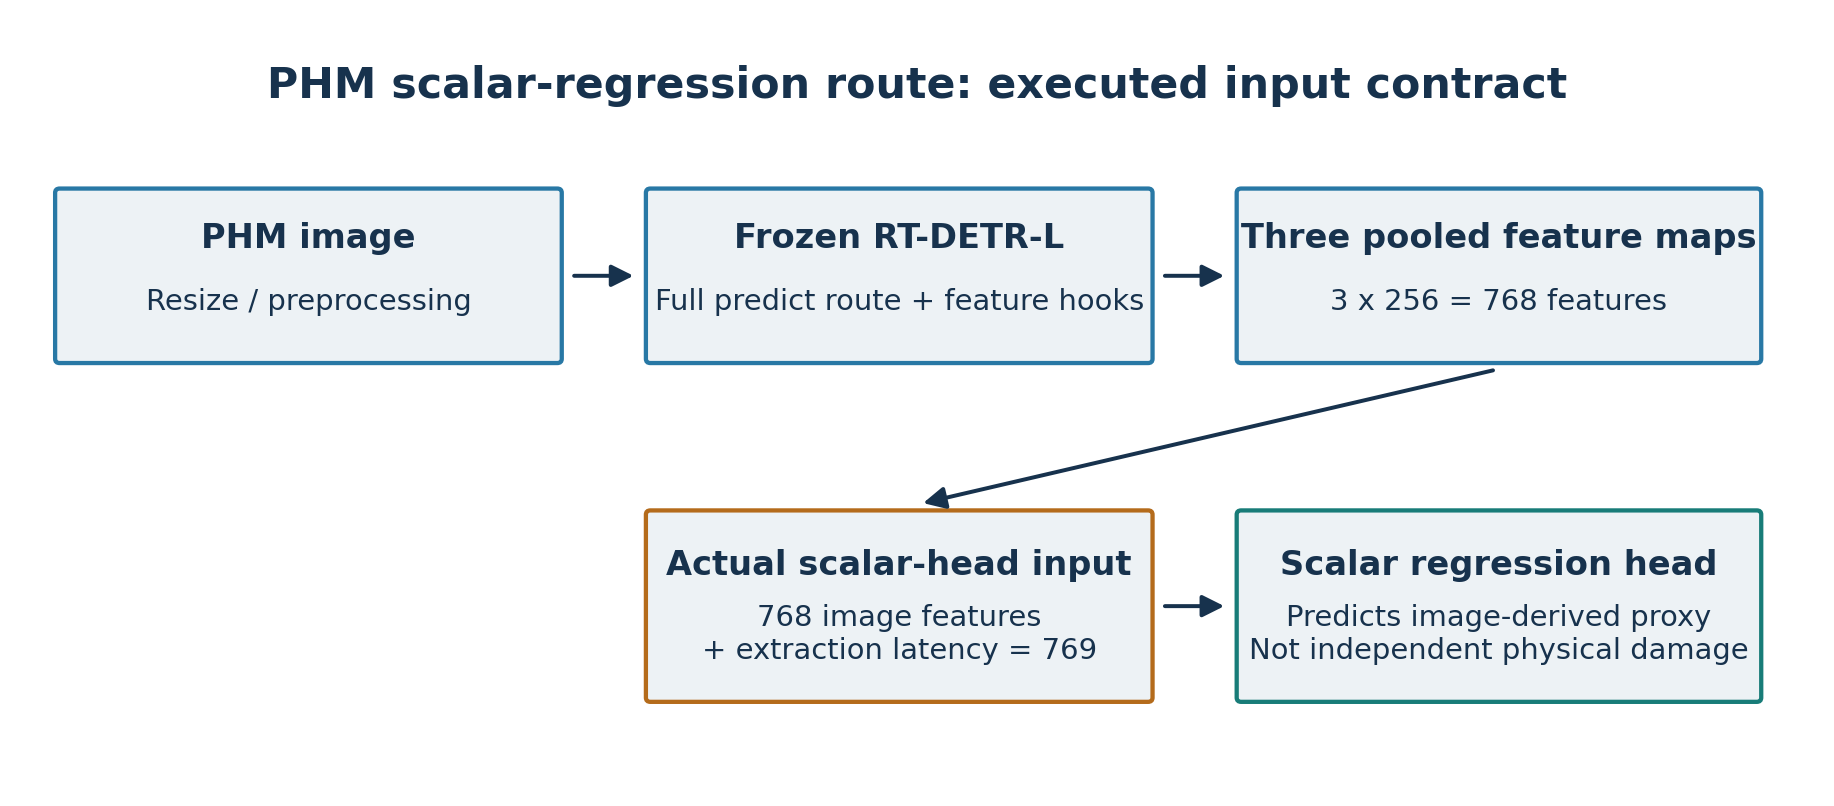
\includegraphics[width=\textwidth]{figures/phm_executed_route.png}
\displaynote{The extraction code adds latency to the 768 image features, producing a
769-dimensional input to regression.}
\end{figure}

\subsection{Assessment Procedure and Available Reference Evidence}
Prediction error measures how well a model reproduces the target on held-out images,
teeth or runs under the specified split. The separate appearance assessment compares
selected images with human judgments. A continuous physical-area reference would require
independent measurements or area annotations. The retained appearance-based and
AnomalyDINO-style diagnostics, which compare pretrained DINOv2 visual features for anomaly detection, are useful for finding conspicuous disagreements, but
their selection and development exposure prevent treating them as an untouched
validation cohort.

The retained evidence contains no independent expert area masks or physical reference
measurements that establish population-wide target accuracy, calibrated area percentages
or a defensible damage/no-damage operating threshold. A prediction cannot independently
resolve ambiguity in the appearance used to construct its training label. These limits
constrain subsequent interpretation even if a target-emulation score appears
favourable.\ev{Photographic proxy and appearance diagnostics}{\EvidenceRef{E020}{}}

\subsection{Target Scaling and Validation Limits}
The two reported baseline errors refer to different versions of the photographic target.
Under the fixed EXP-B-to-EXP-F comparison, the training-mean run MAE is 0.6797
percentage points for v2 and 0.7348 for v3. The difference follows target construction,
not scalar-versus-profile aggregation: the top-three mean of the mean sorted training
profile equals the corresponding scalar training mean by linearity.

The separate v2 EXP-F scalar regression achieved image MAE 0.8939 on 224 images
and raw top-three run MAE 1.3474 on eight runs. The multitask experiment achieved
0.7330 and 1.6273 on those respective units. At confidence 0.60 and IoU 0.50,
the detector returned TP=0, FP=0 and FN=9,883 against the heuristic boxes on 224 test
images; this operating-point failure is distinct from low-confidence ranked detection
AP. In this separate pseudo-box detector experiment, validation selected the first
fine-tuning epoch after four fine-tuning epochs had been completed. The selected
checkpoint epoch therefore does not give the number of epochs trained. These are v2
visual diagnostics, not paired v3 sensor-LOEO results.\ev{Separate
visual diagnostic scores}{\EvidenceRef{E022}{}, \EvidenceRef{E034}{}}

The blind appearance report records agreement on 30 of 38 determinate images (78.9\%),
after four unsure exclusions from 42 proxy-selected extremes. The best of twenty
DINOv2 self-supervised visual-feature configurations agreed on 29 of those 38 (76.3\%). One reviewer, selection of
extremes and reuse of the same judgments for configuration comparison preclude
population-wide validation or a claim of established method superiority.\ev{Selected
appearance checks}{\EvidenceRef{E020}{}}

Detector diagnostics report very small attainable recall against dense heuristic boxes
and a mismatch between predicted-box and pseudo-box scales. Those observations qualify
this training recipe and supervision geometry. Activation energy near an apparent
surface region does not independently prove correct localisation or identify a unique
causal failure mechanism. Likewise, the saved image-regression row included in a later
summary is explicitly not LOEO and lacks EXP-B predictions. Its assessment population
therefore differs from that of the twenty-run sensor LOEO comparison. The retained
visual work establishes reproducible implementation and consequential supervision
limitations, rather than verified physical damage detection.\ev{Training-mean errors by
target version}{\EvidenceRef{E021}{}}\ev{Detector diagnostics}{\EvidenceRef{E034}{}}

\section{Investigation B: Sensor-Based Condition Prediction}
The sensor investigation asks whether run-level inputs available without post-run
imaging predict the provisional condition statistic. Images supply supervision in this
task, not a deployable inference branch. The comparison includes a training-mean
constant, a single sensor encoder and combinations of sensor-feature groups. Maintaining
that distinction prevents the broad phrase ``multimodal fusion'' from obscuring a change
in experimental question. A successful result would establish prediction of a particular
proxy under a particular split. A failed result leaves several possible explanations,
including target noise, acquisition shift, limited independent training support,
representation loss and optimisation limits. The observed comparison alone does not
identify which explanation dominates.\ev{Sensor and fusion
implementation}{\EvidenceRef{E030}{}}

\subsection{Inputs and Preprocessing}
The retained minute-feature configuration names nine base variables: speed, torque,
temperature, axial RMS, radial RMS, and four organiser-provided condition-indicator
channels labelled FM4, NA4, M6A and ALR. These channel names identify supplied
indicators, not independently measured damage labels. Seven summaries per base
variable---mean, standard deviation, median, minimum, maximum, last value and
slope---plus one missingness indicator per variable yield
$9\times(7+1)=72$ channels. These are variable-length
sequences of engineered features. They are not 72 raw accelerometer channels or a
raw-waveform Transformer input. A separate spectral analysis constructs a 72-feature
array from high-frequency vibration.

The custom PHM model forms shared channel-wise patches and applies positional encoding,
a Transformer encoder and masked pooling. Padding and any-valid-time patch masks are
explicit in source. Their existence does not prove historical invariance to batch length
or resolve earlier patch-grid concerns. The principal LOEO runner fits its transformations within each training fold.
The feature definition is anchored to the sensor-feature implementation and retained
fusion configuration. The historical fixed-split experiment fitted the three-group fusion model.\ev{Minute-feature implementation and configuration}
{\EvidenceRef{E124}{}}\ev{Historical fixed-split model identity}
{\EvidenceRef{E025}{}}\ev{Patch and mask
computation}{\EvidenceRef{E029}{patchify}}

\subsection{Reference Predictors and Model Configurations}
The training-mean constant is essential because the target scale and between-experiment
distribution can make a visually plausible prediction uncompetitive. Ridge regression is a supplementary regularised run-summary reference; its historical
v2 fixed-split result is recorded separately in Appendix~\ref{app:supplementary-results}, Section~\ref{sec:phm-ridge-supplement}.
It is not an additional row in the principal v3 LOEO comparison. The custom PatchTST scalar path uses width 32,
two encoder layers, four heads, feed-forward width 64, patch length 16 and stride 8 in
the retained configuration. An optional profile head constrains outputs to sorted
ascending tooth statistics through positive increments; it does not preserve positional
tooth identity.

The retained \texttt{fused\_all\_three} gives context, RMS and condition-indicator
groups separate encoders, concatenates their embeddings and applies a scalar head. This
is feature-level multi-source sensor fusion despite the class name
\texttt{LateFusionRegressor}; neither probability stacking nor visual--sensor inference
describes this path. Figure~\ref{fig:workflow-phm-feature-fusion} shows this
sensor-group concatenation. The later four-arm code additionally distinguishes two RMS sources
and an empty encoder group, which is excluded. Its process-conditioned fusion derives
allocation from context features. These comparisons do not supply the unavailable
inference-time tooth image. Configured epoch caps remain separate from actual fold
histories.\ev{Regression and Ridge implementation}{\EvidenceRef{E030}{}}\ev{Group provenance and
gate}{\EvidenceRef{E028}{}}

\subsection{Training and Evaluation Protocol}
The historical fixed split trains on EXP-B, validates on EXP-A and assesses EXP-F. It
contains seven training, five validation and eight test runs. The principal retained
LOEO procedure instead rotates the assessment experiment while keeping a separate
remaining experiment for validation: train F/validate B/test A; train F/validate A/test
B; train B/validate A/test F. Thus ``leave one experiment out'' does not mean fitting on
both remaining experiments. Only three experiment identities support this analysis.

The retained runner refits its normaliser on each training experiment; the distinct
four-arm diagnostic is qualified in Section~\ref{sec:phm-diagnostics}. The complete historical training entry points and some fold records were not preserved
with the recorded fixed-fusion and LOEO source revisions. Saved predictions therefore
support result checks but not complete reconstruction of those training runs. The pinned
target identity and saved target values establish that the principal comparison uses v3.
For the separate fixed-split comparison, the recorded practical-improvement criterion
was a reduction of 0.15 percentage points in run-level MAE.\ev{Recorded
source-lineage gap}{\EvidenceRef{E129}{}, \EvidenceRef{E130}{}}\ev{Principal LOEO
runner}{\EvidenceRef{E026}{}}\ev{Target provenance}{\EvidenceRef{E021}{}}

\subsection{Results and Uncertainty}
For the historical fixed split, the selected three-group model achieved MAE 0.6548
percentage points on eight EXP-F runs, against the v3 training-mean error of 0.7348.
The observed improvement was 0.0800 percentage points, below the declared 0.15-point
criterion. The report's paired 95\% interval for model-minus-constant MAE,
$[-0.548, +0.414]$, spans zero. This single fixed-split comparison remains separate
from the twenty-run LOEO summary below.\ev{Historical fixed-split result}
{\EvidenceRef{E132}{}, \EvidenceRef{E129}{}}

Table~\ref{tab:phm-loeo} reports the retained twenty-run summary on the provisional
target scale. Lower MAE and RMSE are preferable; rank correlation addresses ordering
rather than calibration. The constant's nonzero pooled rank statistic reflects changing
fold-specific constants, not informative within-fold ranking.

\begin{table}[htbp]
\caption{PHM Prediction Error Across Held-Out Experiments}\label{tab:phm-loeo}
\centering\small
\begin{tabular}{lrrrr}\toprule
Model & MAE & 95\% interval & RMSE & Spearman\\\midrule
Training-mean constant &0.8042 &[0.5769, 1.0360]&0.9608& $-0.0354$ \\
Single encoder &0.9415 &[0.6754, 1.2264]&1.1337& $-0.2053$ \\
Three-group fusion &0.8238 &[0.5527, 1.1015]&1.0332& $-0.1046$ \\\bottomrule
\end{tabular}
\displaynote{The analysis includes 20 nominal run units. Errors are expressed in
percentage points of provisional candidate area. Run-cluster bootstrap intervals are
conditional on the fitted models.}
\end{table}

Figure~\ref{fig:phm-results} shows the retained error estimates and their uncertainty. The learned models do not improve on the training-mean reference in point MAE.

\begin{figure}[htbp]
\caption{PHM2026 Error Under Leave-One-Experiment-Out Evaluation}\label{fig:phm-results}
\centering
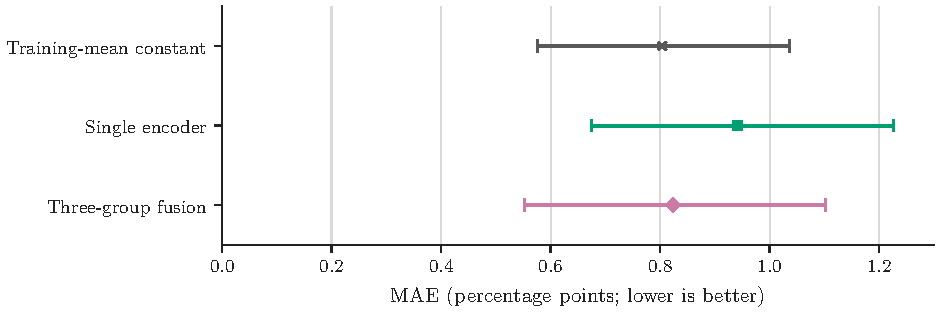
\includegraphics[width=\linewidth]{figures/results_20261128_01/vector/phm_results.pdf}
\displaynote{Points show MAE on 20 nominal run units across three experiments; bars are the retained 95\% run-cluster bootstrap intervals, conditional on the fitted models. These are individual-score intervals, not paired-difference intervals. The target is provisional image-derived candidate area, not independently validated damage.}
\end{figure}

\begin{samepage}
The observed difference in mean absolute error between three-group fusion and the
training mean was $+0.0196$ percentage points across the twenty runs. The mean of the
paired run-bootstrap differences was $+0.0177$ percentage points, with a 95\% interval
of $[-0.1962, 0.2278]$. The interval allows lower error for either predictor. The study
used no prespecified equivalence margin.\ev{Observed errors and paired
bootstrap}{\EvidenceRef{E024}{}}
\par\end{samepage}

\subsection{Interpretation and Limitations}
The retained learned predictors do not establish an improvement over the constant under
this task and protocol. That conclusion is narrower than ``the sensors have no damage
information.'' The target may not align with the physical signal, a model can be
underfit or overfit, and cross-experiment acquisition differences may dominate the small
training population. Twenty nominal runs also do not eliminate dependence caused by
repeated or equal derived sequences.

Run-cluster intervals describe resampling of saved outcomes conditional on fitted
models. They do not quantify full training-seed variation or uncertainty over a
population of independent test machines. With only three experiments, the number of
genuinely different deployment domains remains small. The unresolved target meaning, the
profile's loss of tooth identity and padding/provenance concerns additionally limit
interpretation. These qualifications do not erase a negative comparison; they identify
which hypothesis it actually challenges.\ev{PHM comparison and target
validity}{\EvidenceRef{E104}{}}

\section{Supplementary Diagnostics and Evaluation Sensitivity}
\label{sec:phm-diagnostics}
Supplementary analyses investigate why the original routes were insufficient, without
replacing the principal comparison. The HF/spectral tutorial reports MAE 1.2203 for its
full 72-feature model against a v2 constant MAE 0.6797 on eight EXP-F runs.
Reduced-feature variants performed better than that full model but none beat its
constant. Repeatedly inspecting feature subsets on the same test split makes this a
development diagnostic, not independent confirmation of the selected subset. The feature tables do not isolate overfitting as the cause of the result or establish
byte-level duplication of complete raw archives.

The four-arm study compares group regressors, concatenation, affine late fusion and
context-conditioned embeddings, but fits its normaliser before rotating the folds.
This preprocessing leak prevents treating it as an isolated LOEO assessment or merging
its scores with the principal results. Raw-vibration and tooth-sector screens, AnomalyDINO
sweeps, odd/even views, synthetic controls, teacher/oracle constructions and monotonic
rescoring address separate uncertainties. An oracle or target-derived synthetic feature
can demonstrate pipeline capacity without demonstrating deployable information. The
study-specific records retain these diagnostics with their own target and exposure
definitions; Appendix~\ref{app:supplementary-results}, Section~\ref{sec:phm-fourarm-supplement},
retains the four-arm values separately from the principal comparison.\ev{HF
diagnostic report}{\EvidenceRef{E035}{}}\ev{Four-arm
implementation}{\EvidenceRef{E027}{}}

\section{Synthesis, Limitations, and Motivation for Native-Outcome Paired Studies}
Neither the single sensor encoder nor the three-group model improved on the training
mean in the observed run-level comparison. The paired interval for three-group fusion
included both lower and higher error. Changing the photographic target also changed the
constant predictor's error on a fixed split. The comparison therefore challenges the
inference that adding sensor representations improves prediction of this proxy across
experiments.

Optimising a predictor for physical damage would first require checking the proxy
against independent damage measurements or expert area annotations. Until then, the
error estimates quantify agreement with the photographic rule. The study also leaves
advance warning, remaining useful life and response to natural sensor failure
unresolved. Differences in targets, prediction units and preprocessing prevent a direct comparison
across all PHM fusion models.\ev{Photographic target versions}{\EvidenceRef{E021}{}}\ev{PHM experiment
configurations}{\EvidenceRef{E023}{}}

PHM was undertaken within the architecture programme motivated by robotic welding,
rather than as a prespecified feasibility stage designed around its eventual negative
result. The subsequent move to REASSEMBLE responded to supervision and comparison
limits: recorded action outcomes, visual and sensor inputs at a common completed-action
horizon, and more recording groups. The empirical task changed from a photograph-derived
gear-condition proxy to retrospective manipulation failure, retaining the questions
about representation, fusion and robustness. This progression does not validate a
welding classifier or establish that visual and vibration information are generally
uninformative.

The design lesson is to establish the target, observation horizon and independent
evaluation units before optimising fusion complexity. For PHM, a physical damage
measurement would establish what the proxy represents. The error of the constant
predictor provides a reference for interpreting model performance under degradation. The
subsequent study compares combined pipelines with their single-input reference models
and measures their responses to controlled corruption.\ev{Cross-study
rationale}{\EvidenceRef{E104}{}}

\chapter{REASSEMBLE Case Study: Representation, Fusion, and Robustness}
\label{ch:reassemble}
REASSEMBLE is the central study of completed-action failure classification, comparing
representations, fusion and controlled robustness on paired camera and sensor inputs.
Static F2 improved failure ranking over its statistical sensor component, but combines
visual information with an additional logistic fitting stage and did not establish an
advantage over equal averaging. The original gates did not establish consistent clean
or robustness superiority. Later representation and adaptation studies retain their own
controls and assessment populations; their best results were not combined into one
model.\ev{Core and follow-up scope}{\EvidenceRef{E044}{}, \EvidenceRef{E040}{}}

\section{Study Objectives and Research-Question Mapping}
SQ1 concerns implemented visual and temporal representations relative to engineered
sensor statistics. SQ2 concerns early, late and adaptive fusion under shared recording
groups. SQ3 distinguishes known missing modalities, synthetic degradation of a present
modality and broader distribution shifts. SQ4 concerns the controls needed to interpret
these comparisons: native labels, group separation, inner selection, calibration, paired
uncertainty and computational budgets. The evaluation therefore includes simple
reference predictors and a strong unimodal competitor before interpreting multimodal
gains.

The task is retrospective classification of an already completed action. It is relevant
to monitoring and automated inspection of industrial manipulation, but it is not a
direct replication of rotating-machine damage diagnosis. The observation horizon
includes the action's end. Consequently, a representation that exploits late frames can
be useful here without demonstrating prediction before an unsuccessful event. The
dataset paper supplies acquisition context; the retained manifests and implementation
establish this thesis's specific population and task
\parencite{Sliwowski2025REASSEMBLE}.\ev{Action targets and assessment
cohort}{\EvidenceRef{E046}{}}

\section{Dataset, Native Outcomes, and Modality Constraints}
The inventory contains 149 recordings; the retained common cohort contains 4,530
eligible actions from 148 recordings. A failure is one minus the native success
indicator. There are 509 failures, giving positive-class prevalence 0.1124. Failure
frequency differs substantially by action: pick has 98 failures in 1,190 actions;
insert, 243 in 1,156; remove, 146 in 1,096; and place, 22 in 1,088. This makes action
identity a substantive baseline. These filtered counts are distinct from the dataset
paper's broader acquisition counts, because eligibility and task construction define the
analysis population \citep{Sliwowski2025REASSEMBLE}.

The native outcome describes task success, not a spatial defect mask, severity score or
verified physical root cause. One recording can contribute many actions, and actions
from a recording share acquisition context. Counting 4,530 actions as independent
experiments would overstate the amount of independent evidence. Recording identities are
accordingly used for outer splitting and uncertainty resampling.\ev{Population and class
counts}{\EvidenceRef{E046}{}}

\subsection{Modality Availability and Grouping Limits}
The retained modalities are hand-camera images and machine-sensor measurements: three
force channels, three torque channels, two gripper channels, seven joint-effort channels
and seven joint-velocity channels. These twenty-two channels include operating state as
well as direct interaction measurements. Complementarity is thus an empirical question,
because both modalities may encode action identity or progress rather than independent
evidence of failure.

Segment-offset and drift checks could not establish a common timing anchor between the
action annotations and audio, so the predictive experiment excluded the audio branch.
Spoken outcomes were also a documented potential source of label leakage; this risk was
not a demonstrated leakage result. The exclusion therefore does not show that an audio
model failed to learn.\ev{Audio alignment and documented leakage risk}{\EvidenceRef{E041}{},
\EvidenceRef{E004}{section 16.4}} Similarly, seventeen object categories do not establish
seventeen disjoint physical objects. The available
relationship graph did not support a verified object-instance-disjoint test. The
recording-disjoint split evaluates transfer between recordings. Generalization to unseen
objects or sites and hardware-clock synchronization remain untested.\ev{Audio alignment
and object-group feasibility}{\EvidenceRef{E044}{}}

\section{Cohort Preparation, Alignment, and Evaluation Protocol}
Preparation established a common cohort before comparing architecture outputs. Required
information included native action boundaries and outcomes, valid camera correspondence,
sufficient sensor coverage, and a recording-group identity. These checks support
comparable inputs and prevent changing the evaluation population in response to a
particular model's performance. They do not certify that every outcome label is
unambiguous or that every sensor is physically calibrated.

Eligibility checks and representation choices are distinct: temporal pooling changes the
view of an accepted action, whereas missing observations can affect eligibility or
require a missingness policy.\ev{Preparation and common cohort}{\EvidenceRef{E046}{}}

\subsection{Cohort Construction and Exclusions}
The core analysis uses exactly 4,530 common eligible actions and retains one outcome per
action. Inventory recordings and retained recordings are reported separately rather than
treating the unused recording as evidence of unexplained model failure. Actions outside
the four specified types or without usable required observations are outside this
cohort. Exclusion manifests, rather than model-score thresholds, define eligibility.

Later studies sometimes assess only 753 of these actions. That population is the
original outer-fold-zero assessment subset, containing 77 failures in 26 recordings; it
is not a newly acquired independent holdout. Its prevalence, approximately 0.1023,
differs from the complete cohort's prevalence. Because average precision depends on
prevalence and population composition, a 753-action AP cannot be ranked directly beside
a pooled 4,530-action AP as if only architecture had changed.\ev{Core
cohort}{\EvidenceRef{E046}{}}\ev{Populations used in follow-up
comparisons}{\EvidenceRef{E058}{}}

\subsection{Visual--Sensor Correspondence and Action Boundaries}
Sixteen distinct frames are selected deterministically at approximately uniform
positions within each completed action. The selection uses the recorded action interval;
it does not learn where failure begins. Sensor observations are associated with that
same action and resampled to 512 normalized progress positions. These positions are not
a 512-Hz sampling rate. Normalized progress enables fixed-shape fitting across different
action durations while changing the temporal interpretation of features.

Checks establish manifest-level correspondence and acceptable available coverage. They
do not prove sub-frame synchronization from a shared hardware clock. Boundary errors can
affect both modalities jointly, and late visual information may reflect the already
known outcome. The subsequent boundary review and temporal pooling experiment address
parts of this problem, without converting the task into online warning.\ev{Input
construction}{\EvidenceRef{E064}{}}\ev{Boundary-aware follow-up}{\EvidenceRef{E042}{}}

\begin{figure}[p]
\caption{Sampled Frames From a Completed REASSEMBLE Insertion}\label{fig:reassemble-example}
\centering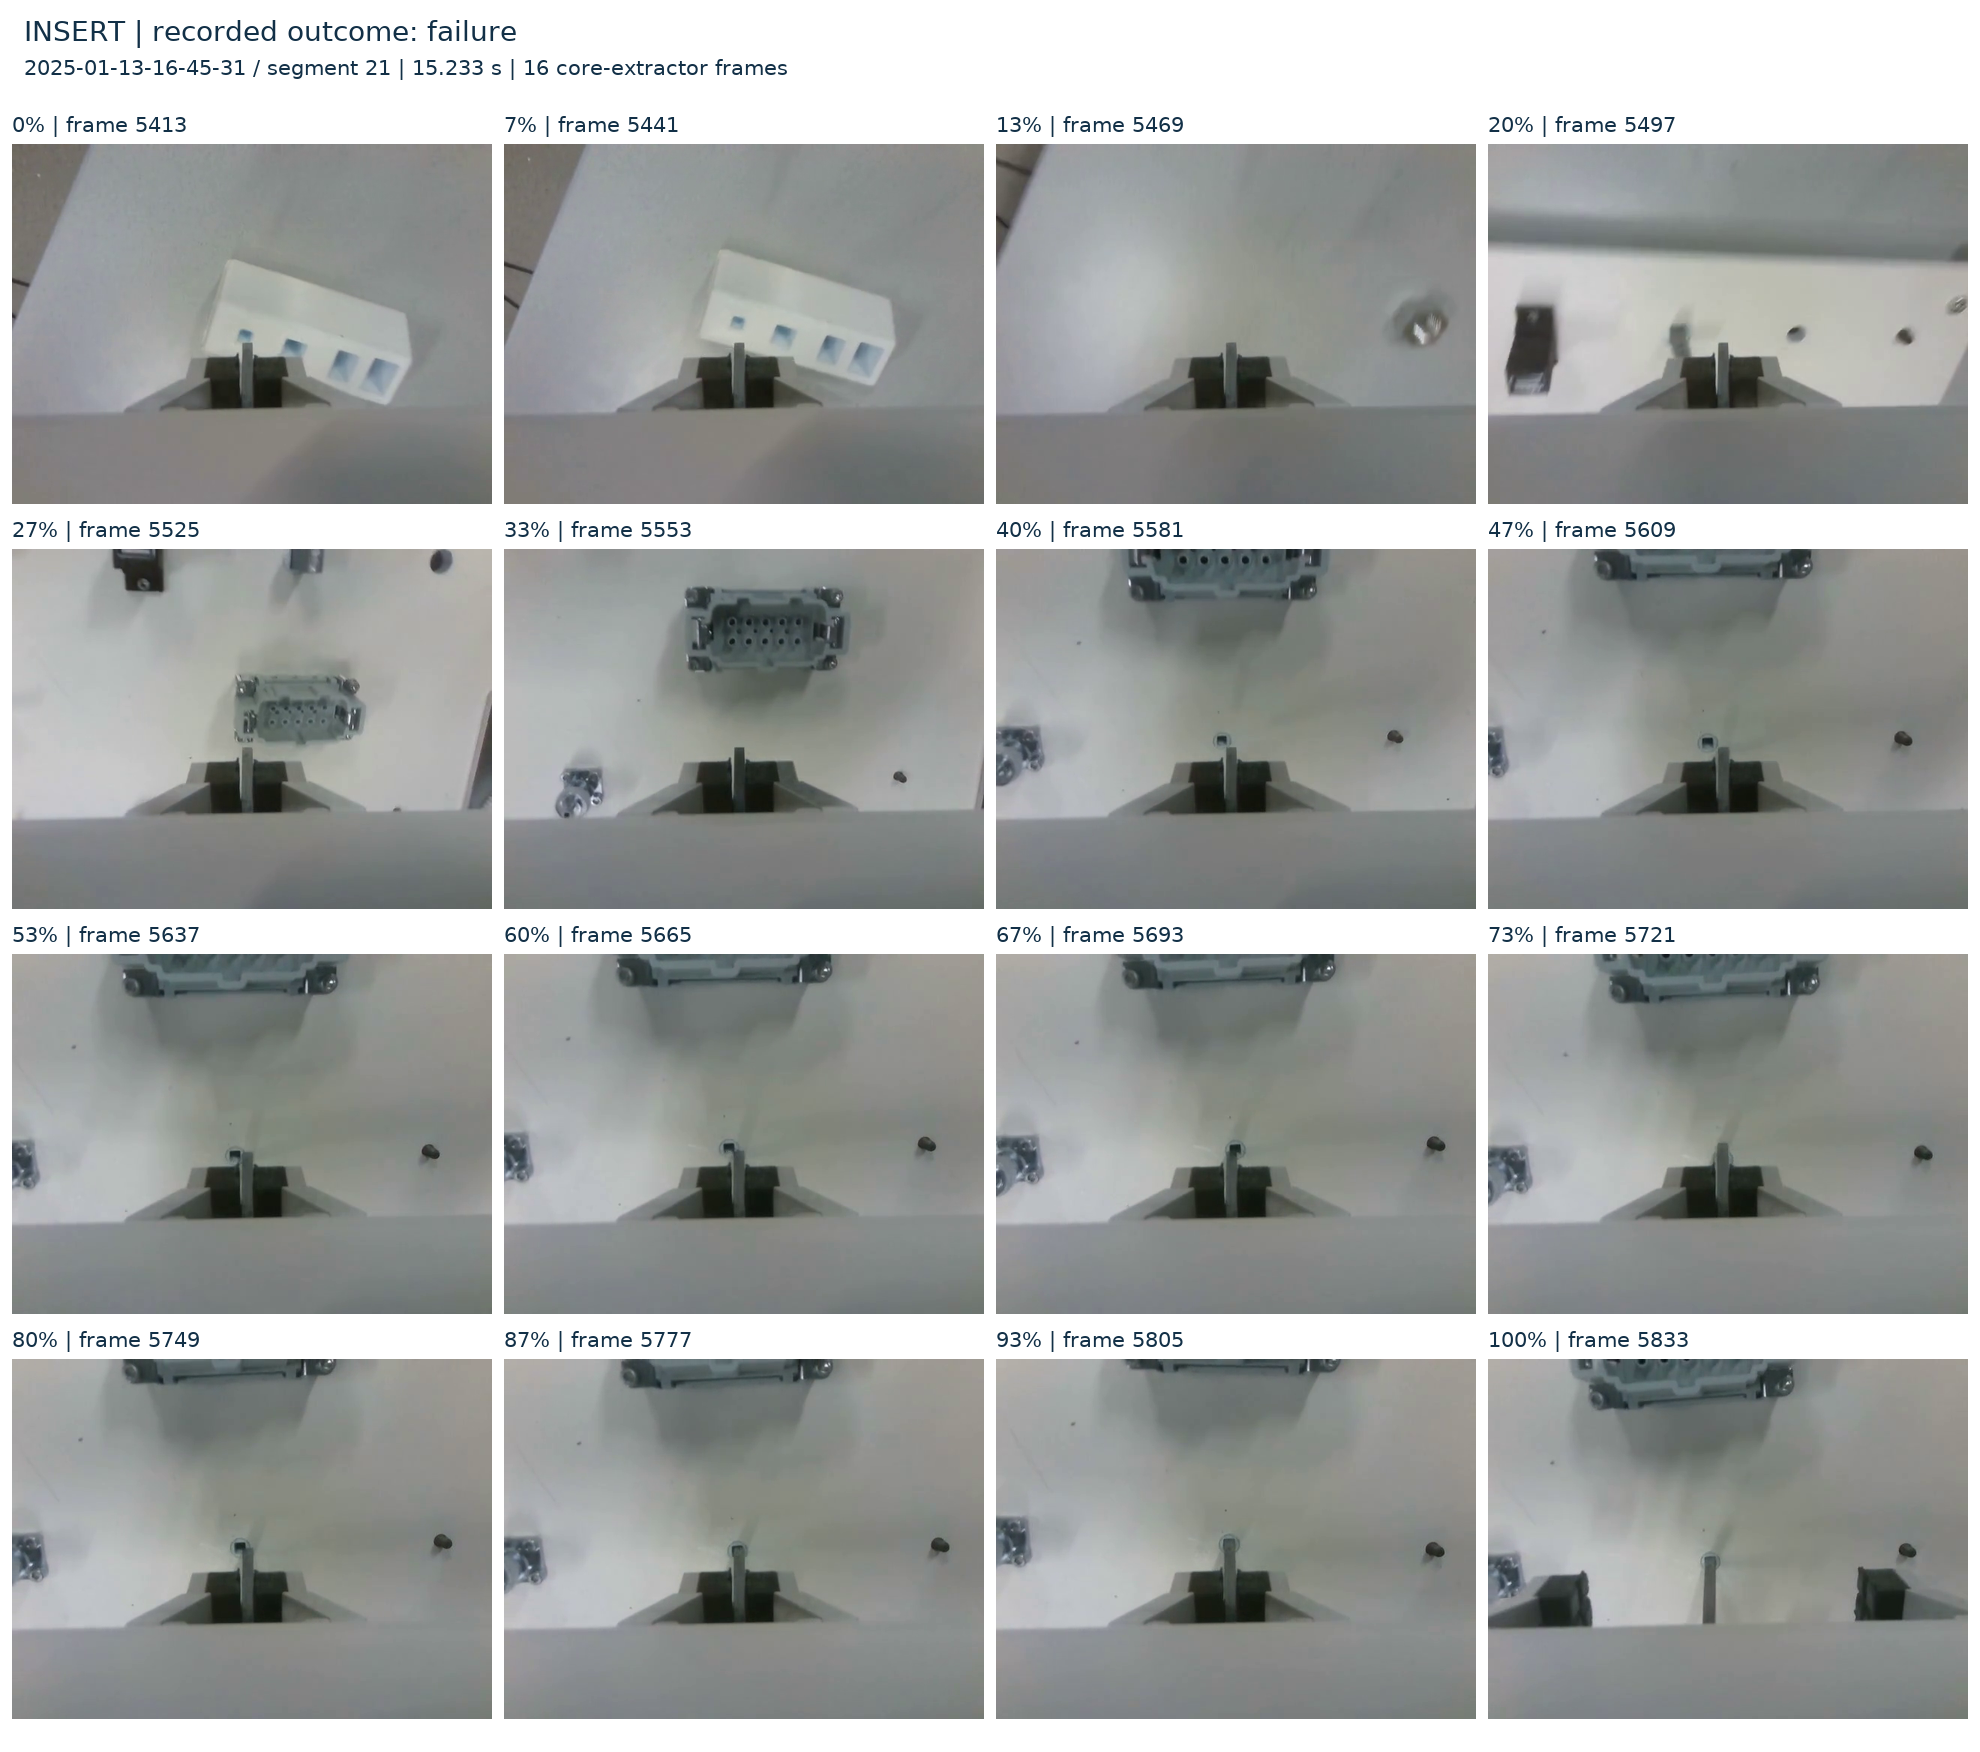
\includegraphics[width=\textwidth,height=.70\textheight,keepaspectratio]{figures/reassemble_example_frames.png}
\displaynote{The extractor selected 16 frames from recording 2025-01-13-16-45-31,
segment 21 (15.233 s). The saved failure label accompanies this example. Frame selection
illustrates temporal coverage. Source: Saved data-preparation example.}
\end{figure}
\ev{Illustrative frame source}{\EvidenceRef{E061}{}}

\subsection{Missing, Invalid, and Inconsistent Observations}
Sensor extraction requires at least 0.89 finite coverage per channel and avoids
extrapolation and interpolation across long gaps. Accepted residual missing values are
filled with training-partition means after channel standardization. Masks remain part of
the input preparation, but the retained PatchTST configuration does not convert the
observed mask into attention suppression. Passing a mask to an API and enforcing
missing-token attention are therefore different claims.

Some proposed quality descriptors have limited information even on clean data. The
gripper median-absolute-deviation outlier statistic is undefined for 1,562 rows and is
imputed from training data; sixteen quality fields are constant on the clean cohort.
Across the saved degraded-input records for all 4,530 actions, fourteen of these fields
changed from their clean value under at least one audited corruption. The fields
\texttt{joint\_efforts.constant\_channels} and
\texttt{joint\_velocities.constant\_channels} remained zero. This check covers the retained
visual-noise, blur, frame-dropout, sensor-noise, channel-dropout, temporal-block and
stuck-force/torque conditions; complete-stream absence is excluded.\ev{Clean quality
fields and saved corruption descriptors}{\EvidenceRef{E048}{}, \EvidenceRef{E152}{},
\EvidenceRef{E153}{}}
% Descriptor check: read only names, row_index and quality arrays from 148 visual/*.npz
% and 148 sensor/*.npz records under implementations/REASSEMBLE/results/runs/
% missing_degraded_modality_robustness/; each condition covers row indices 0--4529.
% Visual: clean, V1_0.02/0.05/0.1, V2_1/2/4, V3_0.1/0.3/0.5.
% Sensor: clean, S1_0.1/0.5/1, S2_0.1/0.3/0.5, S3_0.1/0.3/0.5, S4.
% V4/S5 complete-absence conditions were excluded. Fourteen fields differ from clean
% under at least one condition; this does not imply within-condition variation.

During clean fitting, constant fields provided no variation from which the gate could
learn how changes in those fields related to branch error. This limits interpretation of
the quality inputs but does not establish a causal explanation for the gate results.
Conversely, the deliberate complete-modality-loss experiments supply a known availability
mask, which is stronger information than detecting an unnoticed hardware failure.\ev{Sensor
preparation}{\EvidenceRef{E064}{}}

\subsection{Human Annotation Review and Its Limits}
One reviewer completed 64 selected clips. Of 59 determinate judgments, 57 agreed with
the native outcome and two disagreed; five of 64 were indeterminate. Agreement among
determinate cases is therefore 96.6\%, while agreement over all reviewed cases is
89.1\%. These denominators answer different questions. Sampling balanced action and
label strata with recording spread rather than drawing an unstratified population
sample, so neither proportion is an unbiased dataset-wide error estimate.

For action boundaries, sixty clips were acceptable, three questionable and one
indeterminate; four possible presentation artifacts were also flagged. Overlapping flags
identify ten unique clips requiring adjudication. A single reviewer completed the
assessment. Inter-rater agreement and adjudicated outcomes are therefore unavailable.
Labels, folds and model metrics consequently retain their original definitions; the
review identifies specific uncertainties rather than supplying a replacement ground
truth.\ev{Single-reviewer action and boundary judgments}{\EvidenceRef{E051}{}}

\subsection{Group Definitions and Split Checks}
Five outer folds hold out whole recordings, with four recording-disjoint inner folds for
selection. Outer assessment populations contain 753, 964, 1,037, 906 and 870 actions;
their failure counts are 77, 109, 125, 99 and 99, respectively. The corresponding
recording counts are 26, 31, 32, 29 and 30. Summing the assessment rows recovers all
4,530 actions, 509 failures and 148 recordings exactly.

Within each outer training set, recording-held-out branch predictions supplied the
stacker's OOF bank. Reusing that bank inside stacker validation creates the indirect
dependency explained in Section~\ref{sec:ch4-assessment}; outer-test recordings remain
excluded from branch fitting, calibration, stacker training and threshold selection.
The reported outer scores assess this bank-reuse procedure.\ev{Stacker validation
dependency}{\EvidenceRef{E004}{section 15.4}}

\subsection{Metrics, Calibration, and Conditional Uncertainty}
Failure is positive. Core scores pool the disjoint outer predictions for all 4,530
actions; AP, AUROC, Brier score and fifteen-bin equal-width ECE follow
Section~\ref{sec:ch4-metrics}. Balanced accuracy, macro-F1, failure recall and precision
summarize the selected decisions. Training-only selection and sigmoid logistic calibration use
appropriate inner outputs. Hard-decision thresholds maximize inner balanced accuracy
over 0.01--0.99, with ties resolved toward 0.5. Calibration and threshold selection are
separate operations. Two thousand paired recording-cluster bootstrap resamples quantify
uncertainty conditional on the retained fitted models; they do not refit the entire
procedure or estimate all training-seed uncertainty. Nineteen structured label-shift
permutations preserve recording/action structure under their conditional exchangeability
assumption, giving a smallest plus-one probability of 0.05. The saved controls give observed AP
0.2307 against null AP 0.1435--0.1784 for vision and 0.2416 against 0.1548--0.1876
for PatchTST. Each plus-one probability is 0.05. These conditional controls do not rule
out scene/object shortcuts or replace the paired comparison against action identity.\ev{Metrics and inference
definitions}{\EvidenceRef{E046}{}}

\section{Experiment A: Unimodal Representations}
The unimodal study establishes a reference hierarchy before fusion. Class-prior,
majority and action-type predictors reveal what can be achieved without detailed
observations. Engineered sensor statistics are then compared with the frozen visual
representation and a compact sensor Transformer. Identical retained action identifiers
and recording groups prevent changes in population from masquerading as representation
gains.\ev{Unimodal experiment}{\EvidenceRef{E046}{}}

\subsection{Objective and Comparison Rationale}
The unimodal comparison included simple predictors that can exploit process or sensor
information beyond class prevalence. The action-type predictor controls for the large
native failure-rate differences between pick, insert, remove and place. The
sensor-statistics model controls for useful low-complexity descriptions of force, torque
and motion. The two neural branches test different inductive biases within bounded
budgets; they do not represent exhaustive optimization of all visual or time-series
models.

Both neural branches improved AP over the action baseline. Their AUROC differences
remained unresolved. A later test of incremental predictive value motivated the
visual--sensor fusion comparison.\ev{Neural baselines and incremental fusion
comparison}{\EvidenceRef{E047}{}}

\subsection{Visual Representation Configurations}
The core visual extractor loads the COCO-pretrained RT-DETR-R18vd checkpoint
(\texttt{PekingU/rtdetr\_r18vd}) at the recorded revision. From the loaded detector
instance, it selects \nolinkurl{wrapper.model.backbone.model}, the checkpoint's own
ResNet18-vd CNN backbone, and freezes its parameters. The forward pass reads this
backbone's feature maps and bypasses the hybrid Transformer encoder, detection decoder,
and box heads \parencite{Zhao2024RTDETR}.

Frames follow the shared RGB preprocessing specified in
Appendix~\ref{app:implementation}, Section~\ref{sec:rtdetr-preprocessing}. Spatial means
from three scales concatenate to 896 features per frame; the sixteen frame descriptors
are averaged. A frozen extractor feeds a $896\rightarrow128\rightarrow1$ ReLU/dropout
head with 114,945 trainable parameters. Whole-action averaging discards temporal order.
Weighted binary cross-entropy, AdamW with learning rate 0.001 and weight decay 0.001,
batch size 128 and gradient clipping at one are used. Inner selection chooses five or
ten epochs; outer budgets are 5, 5, 10, 10 and 5.\ev{Executed visual
computation}{\EvidenceRef{E064}{}}\ev{Head and fitter}{\EvidenceRef{E065}{}}

\subsection{Statistical Sensor and PatchTST Configurations}
The statistical representation computes ten features per channel: mean, standard
deviation, median, minimum, maximum, lower and upper quartiles, range, RMS and progress
slope. Twenty-two channels therefore produce 220 features. A training-standardized,
class-balanced L2 logistic model selects $C$ from 0.1, 1 and 10 by mean inner AP. A
subsequent unweighted $C=1$ logistic sigmoid calibrates selected out-of-fold raw scores.

The neural branch is a scratch-trained Hugging Face PatchTST-style model with context
$512\times22$, patch length 32, stride 16, hidden width 32, two layers, four heads and
feed-forward width 64. Internal scaling is disabled; layer normalization and dropout 0.1
are used. Mean patch pooling and channel concatenation feed a 128-dimensional projection
and binary head, giving 109,505 trainable parameters. The observed mask is passed but
does not suppress attention in this configuration. Inner selection allows three or six
epochs and chooses six in every outer fold. This is a compact adaptation of the patching
idea, not a claim to reproduce all settings of the original PatchTST paper
\parencite{Nie2023PatchTST}.\ev{Sensor classification
architecture}{\EvidenceRef{E065}{}}

\subsection{Results and Computational Considerations}
Table~\ref{tab:reassemble-unimodal} reports pooled assessment scores. The majority
predictor has AP equal to prevalence, while the action predictor improves ranking
substantially. Sensor statistics are the strongest retained unimodal representation.
Relative to statistics, PatchTST changes AP by $-0.1878$ with a paired 95\% interval
$[-0.2314,-0.1407]$ and AUROC by $-0.0740$ $[-0.1004,-0.0469]$. Similar trainable head
sizes therefore do not imply similar predictive utility.

\begin{table}[htbp]
\caption{Unimodal Predictions on REASSEMBLE}\label{tab:reassemble-unimodal}
\centering\small

\begin{tabular*}{\linewidth}{@{\extracolsep{\fill}}lrrrrr@{}}\toprule
Model & AP & AUROC & Recall & Brier & ECE\\\midrule
Majority & .1124 & .5000 & .0000 & .1124 & .1124\\
Action type & .1808 & .6851 & .7642 & .0951 & .0080\\
Sensor statistics & .4294 & .7793 & .6149 & .0804 & .0174\\
Frozen visual mean & .2307 & .6978 & .6621 & .0943 & .0070\\
Short-budget PatchTST & .2416 & .7054 & .5639 & .0937 & .0067\\\bottomrule
\end{tabular*}
\displaynote{Scores pool held-out predictions for 4,530 actions. Failure is the positive class.}
\end{table}

The AP intervals are $[.3801,.4828]$ for statistics, $[.1983,.2701]$ for vision and
$[.2102,.2826]$ for PatchTST. The visual pipeline also includes video decoding and
frozen CNN extraction, unlike fitting directly on compact statistics. In the retained
warm-component benchmark, statistical sensors took 26.267 ms, vision 478.415 ms, F2
504.693 ms and F6 564.021 ms. These measurements used a T4, four CPU threads, three
deterministic segments, sensor arrays in memory and cached compressed video; fusion
times are sequential component sums. They establish a bounded practical cost difference
rather than cold-start throughput or a real-time deployment guarantee. Counting only
F2's three learned combination parameters would omit the branch heads and frozen visual
backbone.\ev{Saved unimodal estimates}{\EvidenceRef{E046}{}}\ev{Bounded component
timing}{\EvidenceRef{E043}{}}

\subsection{Interpretation and Implications for Fusion}
Visual AP exceeds the action reference by 0.0499 $[.0225,.0836]$, and PatchTST exceeds
it by 0.0608 $[.0293,.0974]$. Their AUROC differences, 0.0127 $[-.0154,.0406]$ and
0.0203 $[-.0115,.0494]$, remain unresolved. These are metric-specific findings, not
equivalence results. Lower neural AP than sensor statistics also does not exclude
incremental information: useful errors can differ even when one standalone predictor is
weaker.

The fusion experiment therefore uses the statistical sensor predictor as its reference.
The statistical branch was selected for fusion after the initial representation results
were available, so this was an exploratory choice.
Each fitted fusion pipeline is compared with that predictor on the same held-out
actions. The stacker also fits a new logistic map to the branch probabilities. The saved
visual term's contribution to within-fold ordering is examined below. Attribution of the
complete pooled gain remains limited by the absent matched sensor-only second-stage
control. A separate follow-up tests how the training budget affects PatchTST
performance.\ev{Paired unimodal and incremental fusion
comparisons}{\EvidenceRef{E047}{}}

\section{Experiment B: Fusion Strategies}
Six fusion families share the cohort and recording structure: probability averaging,
stacking, representation concatenation and three context-dependent gates. Their input
spaces and calibration stages differ.\ev{Fusion experiment}{\EvidenceRef{E048}{}}

\subsection{Objective and Hypotheses}
The first hypothesis is that the combined visual--sensor pipeline improves held-out
failure ranking relative to the retained sensor pipeline. The second is that action or
quality context improves allocation between branches. These questions are distinct: a
fixed map can use complementary predictions without an effective per-instance
reliability estimate. The comparison changes both inputs and the fitted probability map.
Within-fold ordering can nevertheless identify a visual contribution beyond a strictly
increasing transformation of the sensor score. A matched sensor-only second-stage model,
which was not completed, would strengthen attribution of the full pipeline contrast.
Both sensor-only and simple static fusion references are therefore needed when
interpreting adaptive models.

Clean gains do not establish corruption recognition; the subsequent experiment tests
frozen clean-trained models directly.\ev{Fusion questions and
controls}{\EvidenceRef{E048}{}}

\subsection{Compared Architectures and Exact Fusion Formulations}
F1 averages calibrated probabilities: $p=(p_v+p_s)/2$. F2 fits a fixed-$C=1$ L2 logistic stacker,
\begin{equation}p=\sigma(b+a_vp_v+a_sp_s).\end{equation}
It has three scalar parameters. Its signed coefficients are unconstrained and do not
form convex reliability weights. F3 instead projects the 128-dimensional visual
representation and 220 sensor statistics to separate 128-dimensional vectors,
concatenates and layer-normalizes them, and uses a hidden layer of width 32 or 64.
Candidate training budgets are ten or twenty epochs.

F4--F6 use a masked softmax gate and calibrated branch logits:
\begin{equation}w=\operatorname{softmax}(h(u)+\text{availability mask}),\qquad
p=\sigma\!\left(\sum_m w_m\operatorname{logit}(p_m)\right).\end{equation}
F4 receives four action indicators and two availability indicators. F5 receives
thirty-six quality descriptors and availability; F6 receives all forty-two inputs.
Hidden widths are eight or sixteen. The gates have no final intercept correction or
post-gate calibrator. Context or quality can encode process content as well as
reliability; interpreting a learned weight as causal sensor trust is therefore
unsupported.\ev{Exact implemented fusion links}{\EvidenceRef{E066}{}}

\subsection{Training, Calibration, and Evaluation}
Fusion uses branch prediction banks with recording-excluded row construction and
held-out outer assessment recordings. The internal bank-reuse dependency described above
remains part of its selection procedure. F2 stacks calibrated probabilities, whereas
F4--F6 mix calibrated logits. F2 fixes $C=1$ and has no further calibration stage. F3
uses weighted binary cross-entropy and a sigmoid calibrator; the gates use unweighted
binary cross-entropy, forty epochs, learning rate 0.003 and weight decay 0.001. These
differences in link, objective and calibration opportunity are part of the recipes,
rather than controls that isolate adaptation alone.

Gate results average probabilities from seeds 20260927--20260929. Averaging
probabilities is not equivalent to inserting averaged weights into a sigmoid. The core
threshold protocol and paired recording bootstrap remain in force. These controls
improve comparability but do not equalize every architecture's effective capacity,
objective or calibration opportunity.\ev{Fusion training and nested
banks}{\EvidenceRef{E048}{}}

\subsection{Predictive Results and Uncertainty}
F2 has AP 0.4473 and AUROC 0.7950. The paired differences for F2 minus the statistical
sensor predictor were 0.0179 $[.0086,.0283]$ in AP and 0.0156 $[.0060,.0255]$ in AUROC.
The Brier score difference was $-0.0020$ (95\% CI $[-.0031,-.0009]$), indicating lower
probability error for F2. The ECE difference $-0.0036$ $[-.0127,.0099]$ and recall
difference $-0.0039$ $[-.0255,.0163]$ remain unresolved. The more precise AP contrast is
$+0.017907$ $[.008603,.028284]$. Against probability averaging, F2's AP gain is only
$+0.001556$ $[-.007607,.011165]$, which does not establish a discrimination advantage.
Thus the retained evidence supports a modest combined-pipeline increment over sensors,
with improved probability quality on some metrics, rather than a general superiority of
learned stacking over simple averaging.

\begin{table}[htbp]
\caption{Fusion Results for the 4,530 Matched REASSEMBLE Actions}\label{tab:reassemble-fusion}
\centering\small

\begin{tabular}{lrrrrr}\hline
Model & AP & AUROC & Recall & Brier & ECE\\\hline
F1 probability mean & .4457 & .7951 & .6031 & .0834 & .0355\\
F2 probability stacker & .4473 & .7950 & .6110 & .0784 & .0138\\
F3 representation fusion & .4122 & .7856 & .6385 & .0827 & .0149\\
F4 action gate & .4437 & .7815 & .6031 & .0802 & .0128\\
F5 quality gate & .4445 & .7760 & .6012 & .0806 & .0126\\
F6 combined gate & .4414 & .7755 & .5717 & .0807 & .0124\\\hline
\end{tabular}
\end{table}

All three original gates have lower AUROC than F2, with intervals excluding zero for
those differences. Their AP differences remain unresolved. The AP difference for F6
minus F2 was $-0.0059$ $[-.0248,.0137]$. The failure-recall difference for F6 minus F2
was $-0.0393$ (95\% CI $[-.0649,-.0122]$).\ev{Fusion results and paired
contrasts}{\EvidenceRef{E048}{}}

\subsection{Modality Complementarity and Error Analysis}
At the frozen hard-decision thresholds, both unimodal branches are correct on 2,347
actions and both wrong on 529. Vision alone is correct on 486, while sensors alone are
correct on 1,168. Among 509 failures, 240 are identified by both, 99 by neither, 97 by
vision alone and 73 by sensors alone. Failures detected by vision alone occurred in 61
recordings.

An oracle that always selected a correct branch would identify 410 of 509 failures,
approximately 0.8055 recall. That is an unavailable truth-dependent upper reference, not
an achieved fusion result or a deployable gate. Complementarity provides potential
information, while learning which branch to trust from available inputs remains a
separate problem. These counts describe decisions at fixed thresholds. Paired AP
comparisons assess the ranking of the same actions across thresholds.\ev{Error-overlap
analysis}{\EvidenceRef{E047}{}}

\subsection{Interpretation and Comparison Limits}
Independent saved-prediction recomputation separates within-fold ordering from
cross-fold score alignment. All five F2 sensor coefficients are positive. Omitting the
visual term while retaining the jointly fitted parameters,
$q_{s,k}=\sigma(b_k+\alpha_{s,k}p_s)$, therefore preserves sensor ordering within fold
$k$. Its AP and AUROC match the sensor branch exactly within every fold. Restoring
vision improves AUROC in all five folds and AP in four; the remaining AP difference is
$-0.00469$. Thus, the visual term supplies beneficial observed ordering changes beyond a
strictly increasing transformation of the same sensor probabilities, although its AP
benefit is not uniform. Appendix~\ref{app:supplementary-results} gives the fold-level
check.

Pooled AP is .42939 for sensors, .43092 for the reduced score and .44730 for complete
F2. Different fold-specific maps can change pooled ordering while preserving every
within-fold ranking. This omission is an arithmetic diagnostic, not a refitted
sensor-only control or a missing-modality experiment. It does not uniquely allocate the
pooled gain to vision, establish information conditional on all sensor features, or
quantify causal modality importance. AP changes also do not measure calibration. The
folds share training populations; historical recording-bootstrap intervals condition on
fixed models and omit training and repeated selection uncertainty. These findings do not
establish population-wide superiority or a resolved advantage over equal
averaging.\ev{Independent saved-score verification}{\EvidenceRef{E113}{}}

Within the tested representations and budgets, neither intermediate fusion nor the
original adaptive gates establishes an advantage over the successful static reference.
This finding is architecture- and protocol-specific. The later anchored model changes
the link and learns a different function class; its positive exploratory AP result is
therefore compatible with the original gates' bounded negative evidence.\ev{Original
REASSEMBLE fusion comparisons}{\EvidenceRef{E044}{}}

\section{Experiment C: Missing and Degraded Modalities}
The core robustness study froze the clean-trained statistical sensor and visual
predictors (U1 and U2), equal averaging (F1), the stacker (F2), and the two gates using
quality descriptors (F5 and F6). It perturbed one input at a time and also tested known
loss of a full input stream.\ev{Core robustness study}{\EvidenceRef{E055}{},
\EvidenceRef{E049}{}}

\subsection{Robustness Questions and Tested Conditions}
The central question is whether a gate both changes allocation in the expected direction
and limits predictive deterioration relative to F2. Absolute performance at high
severity is also necessary: a weak clean model can show a small decline merely because
little useful ranking remains to lose. An intact unimodal branch supplies a practical
reference for whether fusion introduces avoidable damage.

Clean decision thresholds remain frozen during corruption. This matches a deployment in
which the operator does not receive fault labels and recalibrate at every severity.
Known availability masks in complete-dropout tests are an explicitly different
information condition. The two sets of results measure responses to different
information about the fault.\ev{Robustness contrasts and decision
policy}{\EvidenceRef{E049}{}}

\subsection{Corruption Operators and Severity Definitions}
Visual operators include pixel Gaussian noise with standard deviations 0.02, 0.05 and
0.10 on the normalized scale, Gaussian blur at severities one, two and four, and removal
of two, five or eight of sixteen selected frames. Sensor operators include Gaussian
noise scaled by 0.1, 0.5 or 1.0 training-channel standard deviations; removal of two,
seven or eleven channels; missing temporal blocks covering 10\%, 30\% or 50\% of the
sequence; and six force/torque channels stuck at training medians.

Sensor statistics and quality descriptors are recomputed from the altered input, rather
than retaining clean summaries beside corrupted signals. The core uses its fixed
operator realization protocol. A later augmentation study averages across five
stochastic test realizations. Its Gaussian-noise estimates therefore refer to a
different evaluation protocol. None of these operators is direct evidence of
cross-machine shift, clock drift or physical sensor recalibration.\ev{Operator
implementation and severities}{\EvidenceRef{E049}{}}

\subsection{Missingness Policies and Dropout Experiments}
In the original complete-dropout test, the four evaluated fusion models used the
statistical sensor probability and threshold when vision was absent. When sensors were
absent, they used the visual predictor and its threshold. The evaluator received the
identity of the missing stream. The core gate rejects a sample with both streams absent.
The robustness report contains no empirical result for that condition. A later
quality-interaction pilot marked such predictions unavailable.

A separate F6 training experiment samples visual-only dropout with probability 0.15,
sensor-only dropout with probability 0.15 and both-present inputs with probability 0.70.
Both-absent inputs are never sampled. Because a one-available-modality softmax has
weight exactly one and the branches are fixed, its missing-case output is structurally
fixed and supplies no useful gradient for improving the fallback prediction. Dropout
training cannot make that output better under this architecture. Its clean AP is 0.4377,
changing ordinary F6 by $-0.0037$ $[-.0085,.0003]$.\ev{Explicit fallback and
dropout}{\EvidenceRef{E045}{}}

\subsection{Predictive Performance and Calibration Under Degradation}

Table~\ref{tab:reassemble-corruption} reports every declared operator at its strongest
severity and the two known single-stream absence cases. All rows use the same core
cohort and fixed clean models. The accompanying robustness report contains the
intermediate-severity results.\ev{Intermediate-severity results}{\EvidenceRef{E049}{}}

\begin{table}[htbp]
\caption{REASSEMBLE High-Severity Corruption and Known Absence}
\label{tab:reassemble-corruption}
\centering\small\setlength{\tabcolsep}{3pt}
\begin{tabular}{lrrrrrr}\toprule
Condition & Intact AP & F2 AP & Brier & ECE & F5 AP & F6 AP\\\midrule
Pixel noise ($\sigma=.10$) & 0.4294 & 0.3963 & 0.2968 & 0.4368 & 0.1288 & 0.1275\\
Blur ($\sigma=4$) & 0.4294 & 0.4099 & 0.0816 & 0.0146 & 0.4061 & 0.4179\\
Frame removal (8/16) & 0.4294 & 0.4455 & 0.0786 & 0.0149 & 0.4392 & 0.4381\\
Sensor noise ($1\,\mathrm{SD}$) & 0.2307 & 0.2222 & 0.4798 & 0.5251 & 0.1753 & 0.1788\\
Channel removal (11/22) & 0.2307 & 0.3198 & 0.0899 & 0.0164 & 0.3183 & 0.3014\\
Temporal block (50\%) & 0.2307 & 0.3490 & 0.0918 & 0.0421 & 0.3543 & 0.3267\\
Stuck force/torque (6) & 0.2307 & 0.4396 & 0.0822 & 0.0237 & 0.4230 & 0.4211\\
Vision absent & 0.4294 & 0.4294 & 0.0804 & 0.0174 & 0.4294 & 0.4294\\
Sensors absent & 0.2307 & 0.2307 & 0.0943 & 0.0070 & 0.2307 & 0.2307\\
\bottomrule\end{tabular}
\displaynote{Pooled failure-positive AP on 4,530 actions (509 failures). Brier and ECE
refer to F2; smaller values indicate less probability error. Intact AP is statistical
sensing for visual faults and vision for sensor faults. Known absence routes all three
fusion methods to that survivor. The stochastic realization protocol is the original
core protocol, distinct from later augmentation studies.}
\end{table}
\ev{Saved core robustness estimates and arithmetic checks}{\EvidenceRef{E138}{},
\EvidenceRef{E141}{}, \EvidenceRef{E055}{}}

Under strongest pixel Gaussian noise, F2 retains AP 0.3963, while F5 and F6 fall to
0.1288 and 0.1275. The intact sensor baseline remains at AP 0.4294. F2's Brier score
nevertheless rises to 0.2968 and ECE to 0.4368, compared with clean sensor values 0.0804
and 0.0174. Ranking retention therefore conceals severe probability failure.

Under sensor Gaussian noise at one training standard deviation, F2 AP is 0.2222 and
F5/F6 are 0.1753/0.1788, below intact vision at 0.2307. F2's Brier/ECE rise to
0.4798/0.5251. Strong blur gives F2/F5/F6 AP 0.4099/0.4061/0.4179, without a resolved
general gate advantage. These conditions demonstrate that combining an intact and
corrupted modality can underperform the intact branch. Detection of corruption and
calibrated uncertainty remain unresolved rather than being supplied automatically by a
fusion layer.\ev{Core high-severity metrics}{\EvidenceRef{E049}{}}

\subsection{Gate Behaviour and Fallback Behaviour}
No tested original gate/family combination establishes both an appropriate allocation
response and a smaller decline under the study's criteria; no supported absolute
high-severity AP superiority follows. A gate weight can change with a quality input
without changing in a beneficial way. Conversely, a smaller performance decline from a
weaker clean starting point is insufficient to establish improved reliability.

Exact missing-modality equality follows programmed fallback. It demonstrates consistent
handling of known absence, while corruption recognition and useful recovery remain
separate capabilities. This is narrower than training an encoder or student to retain
performance after input loss, as in transferable missing-modality methods
\citep{P005,P007,P016}.\ev{Gate allocation and fallback audit}{\EvidenceRef{E049}{}}

\subsection{Interpretation and Untested Conditions}
The core evidence rejects a broad claim of reliable adaptation for the tested gates. The
AP, calibration and intact-branch comparisons capture different consequences of
corruption. Robustness to known complete absence is largely architectural here;
robustness to unnoticed corruption is empirically weak.

Natural missingness mechanisms, simultaneous partial failures, asynchronous clocks, new
machines, new operating sites and prospective early warning were not established. The
later augmentation study changes training exposure and tests several held-out operator
families, but the same recording population and already observed core faults limit
claims of independent discovery. An untested condition remains open rather than
receiving a favorable interpretation from the model's name.\ev{Tested missingness and
corruption conditions}{\EvidenceRef{E044}{}}

\section{Controlled Follow-up Investigations}
\label{sec:reassemble-followups}
Table~\ref{tab:reassemble-followups} maps the follow-ups to their assessment population
and matched control. Rows with different fitting recipes or populations are not a
leaderboard. The subsections retain the full definitions and qualifications.

\begin{table}[p]
\caption{REASSEMBLE Follow-up Populations, Controls, and Outcomes}
\label{tab:reassemble-followups}
\centering\footnotesize\setlength{\tabcolsep}{3pt}
\begin{tabularx}{\linewidth}{@{}P{.18\linewidth}P{.12\linewidth}YP{.27\linewidth}Y@{}}\toprule
Investigation & Actions / recordings & Matched control & AP contrast [95\% interval] & Status and scope\\\midrule
Sensor budget & 4,530 / 148 & Short-budget PatchTST & Long minus short: $+.0297$ [$+.0122,+.0451$] & Completed; remains below statistics\\\addlinespace
Sensor hybrid & 4,530 / 148 & Statistics & Hybrid minus statistics: $+.0110$ [$+.0054,+.0181$] & Completed; same sensing modality\\\addlinespace
Temporal pooling & 4,530 / 148 & Whole-action mean F2 & Last-quarter F2 minus control: $+.0461$ [$+.0260,+.0632$] & Completed; 16 frames; selected same-cohort follow-up\\\addlinespace
Spatial encoder & 4,530 / 148 & CNN-only F2 & Hybrid-encoder F2 minus CNN F2: $-.0158$ [$-.0248,-.0058$] & Completed; 16 frames; five-epoch heads\\\addlinespace
Two-epoch tuning & 4,530 / 148 & Frozen32 F2 & Tuned32 minus frozen32, seed 42: $-.0008$ [$-.0064,+.0061$] & Two seeds completed; both F2 contrasts unresolved\\\addlinespace
Twenty-epoch CNN & 4,530 / 148 & No completed matched F2 & Visual AP .3121; no paired F2 interval & One seed completed; two seeds deferred; F2 unexecuted\\\addlinespace
Hundred-epoch screen & 753 / 26 & Matched frozen100 F2 & Full100 minus frozen100: $+.0141$ [$-.0008,+.0291$] & One seed/role; unresolved; resource account below\\\addlinespace
Anchored adaptation & 4,530 / 148 & Matched F2 anchor & Adaptive minus anchor: $+.0210$ [$+.0015,+.0419$] & Completed; independent of pooling changes\\\addlinespace
Matched augmentation & 4,530 / 148 & Augmented static F2 & Adaptive minus static, mean conditions: $+.0097$ [$-.0034,+.0228$] & Completed; primary effect unresolved\\\addlinespace
Quality-interaction pilot & 753 / 26 & Exposure-matched static A & C minus A, mean Gaussian AP: $+.0030$ [$-.0267,+.0322$] & Completed single-fold pilot; unresolved\\\bottomrule
\end{tabularx}
\displaynote{Intervals are paired and conditional on fixed fitted models. Ordinary
rows use pooled failure AP; the two corruption rows average condition-specific APs,
with their own realization protocols. Frames and fitting budgets differ. Resource
screens and fine-tuning rows describe separate scopes, not a completed common matrix.}
\end{table}
\ev{Follow-up controls and scopes}{\EvidenceRef{E038}{}, \EvidenceRef{E039}{},
\EvidenceRef{E040}{}, \EvidenceRef{E042}{}, \EvidenceRef{E058}{}, \EvidenceRef{E059}{},
\EvidenceRef{E062}{}}

Three exploratory comparisons on the same cohort yielded higher average precision under
their respective protocols. Last-quarter visual pooling with static stacking reached
0.4934, anchored adaptation reached 0.4683, and combining long-budget PatchTST with
sensor statistics reached 0.4403. Each had its own control. The temporal-pooling study
was completed separately from an earlier visual experiment that stopped after partial
execution. Other follow-ups examined matched corruption exposure and visual
tuning.\ev{REASSEMBLE follow-up experiments}{\EvidenceRef{E040}{}}

\subsection{Longer Sensor Training and Alternative Sensor Representations}
The longer-budget experiment retains the PatchTST inputs and architecture, permits up to
one hundred epochs, and uses minimum ten epochs with patience twelve. No long-budget
inner fit reaches the cap; outer budgets use rounded median inner best epochs. Against a
matched short-budget control, AP rises from 0.2557 to 0.2853, a difference of 0.0297
$[.0122,.0451]$. The original short-budget experiment yielded 0.2416 AP under its own
protocol.

Long training remains below statistics: AP difference $-0.1441$ $[-.1861,-.1009]$. A
fixed-$C=1$ stacker combining long PatchTST and statistics reaches AP 0.4403, improving
statistics by 0.0110 $[.0054,.0181]$. This combines two representations of the same
sensor modality. It qualifies the original budget-dependent neural result while
preserving the strong engineered baseline.\ev{Matched sensor-budget
experiment}{\EvidenceRef{E040}{}}

\subsection{Alternative Visual Pooling}
The boundary-aware experiment exactly reproduces the original whole-segment mean before
changing pooling. AP is 0.2556 for two halves, 0.3080 for thirds, 0.3191 for the last
quarter, 0.2922 for early-plus-late and 0.2250 for an ordered GRU. The original mean is
0.2307. Last-quarter minus mean AP is 0.0885 $[.0424,.1293]$; the protocol's
simultaneous lower bound across five AP contrasts remains positive at 0.0301.

The last-quarter and whole-action means use equally sized fitted heads, so additional
head parameters cannot explain their contrast. Concentrated outcome cues or less
dilution are plausible explanations, but neither mechanism was isolated.

This supports selected temporal aggregation changes, not a general recurrent-model
advantage or an isolated causal effect of temporal order. The GRU changes capacity and
inductive bias, while bin concatenation changes classifier inputs. The selected
last-quarter rule exploits complete-action information. Its separate F2 follow-up
reaches AP 0.4934, with the more precise value 0.493437 versus original F2 0.447299:
difference $+0.0461$ $[.0260,.0632]$, and AUROC difference $+0.0403$ $[.0291,.0522]$.
This is a meaningful exploratory same-cohort result after representation selection, not
independent confirmation or warning before the outcome. It was not combined with the
anchored adaptive gate or the same-sensor hybrid.\ev{Visual pooling definitions and
paired comparisons}{\EvidenceRef{E042}{}}

\subsection{Spatial-Encoder and Backbone Comparisons}
A separate five-fold comparison tests CNN-only against CNN plus the spatial hybrid
encoder, with the same sixteen frames, 4,530 actions, frozen extraction and five-epoch
heads. It uses its own fitting and calibration subsets. CNN-only visual AP is 0.221644
and F2 AP 0.440764; hybrid-encoder visual AP is 0.171915 and F2 AP 0.424979, with shared
sensor AP 0.420926. The hybrid-minus-CNN F2 difference is $-0.015785$
$[-0.024804,-0.005800]$. Executing more of the detector therefore worsens this
particular comparison, rather than automatically improving representation
quality.\ev{Matched spatial-component results}{\EvidenceRef{E039}{}}

The descriptors also differ in width: CNN multiscale pooling yields 896 features and the
spatial hybrid-encoder path 768. Head size, active components and compute change with
that representation. The result cannot isolate an attention effect, and the attention is
spatial rather than across video time. Neither path executes the object-detection
decoder. CNN-only extraction, spatial-encoder extraction, final-stage tuning and
complete detector training remain distinct interventions.\ev{Architectures in the
spatial-component comparison}{\EvidenceRef{E057}{}}

\subsection{Frozen Versus Fine-Tuned Visual Representations}
An earlier four-arm comparison used sixteen or thirty-two frames, with frozen CNN
features and five-epoch heads, or final-stage CNN adaptation and two-epoch heads. The
adapted arms jointly fitted the head and final CNN stage; earlier CNN weights and
normalization buffers remained fixed. The unequal epoch budgets prevent attributing the
contrast to adaptation alone. Table~\ref{tab:fourarm-visual-supplement} in
Appendix~\ref{app:supplementary-results} gives the four results.\ev{Earlier four-arm
comparison}{\EvidenceRef{E146}{}, \EvidenceRef{E147}{}}

The subsequent matched diagnostic uses thirty-two frames and two epochs for both arms
across the full 4,530-action cohort and two seeds. It adds seventy-five fits and reuses
all twenty-five seed-42 fits from the earlier two-epoch fine-tuned32 arm: four inner
fits and one final fit for each of five outer folds. These reused fits are not an
independent replication. Epoch matching does not imply compute matching. The follow-up
sensor reference has pooled AP 0.4208, distinct from the core selected-$C$ baseline's
0.4294.\ev{Matched comparison and fit lineage}{\EvidenceRef{E062}{},
\EvidenceRef{E145}{}}

For seed 42, visual AP changes from 0.2227 to 0.2306, but the difference 0.0079 has
interval $[-.0173,.0332]$; F2 changes from 0.4394 to 0.4386. For seed 20261023, visual
AP changes from 0.2168 to 0.2005, and F2 from 0.4352 to 0.4324. The corresponding paired
intervals include zero. These results do not identify a unique cause for the absence of
a fusion gain, such as calibration or out-of-fold mismatch; two seeds also do not fully
characterize seed variability.\ev{Matched two-epoch diagnosis}{\EvidenceRef{E062}{}}

The later twenty-epoch visual cap completes twenty inner and five outer fits for seed
42. Pooled visual AP is 0.3121, while mean fold AP is 0.3086. The additional fifty fits
for two more seeds were not evaluated, leaving variability across seeds unmeasured
for this configuration. Twenty-epoch F2 was not executed because its controller expected the
larger bank. The retained checkpoint validator's twenty-five-source-epoch requirement
conflicts with the twenty-epoch donor; that is an eligibility/configuration conflict,
not evidence of failed training.\ev{Completed twenty-epoch fits}{\EvidenceRef{E059}{}}

The hundred-epoch pilot restarts both arms from pretrained weights with fresh heads,
rather than continuing the twenty-epoch run. Both arms execute one hundred epochs and
select epochs fourteen (frozen) and forty-seven (full). On the same 753-action
assessment subset, visual AP is 0.1938/0.2126 and F2 AP 0.3350/0.3491. Full-minus-frozen
F2 AP is 0.0141 $[-.0008,.0291]$, leaving the difference unresolved. Restricted
historical F2 is 0.3672 on these same rows; its full-cohort AP is not the relevant
comparator.\ev{Matched pilot assessment cohorts}{\EvidenceRef{E058}{}}

\subsection{Adaptive-Fusion Extensions and Matched Controls}
Anchored adaptation preserves the successful F2 link and learns bounded adjustments:
\begin{equation}p=\sigma\!\left(b+\sum_m a_m[1+\tanh(h_m(u))]p_m\right).\end{equation}
The adaptive network is $42\rightarrow16\rightarrow2$ with zero final-layer
initialization; a two-parameter constant adjustment is a matched control. AP reaches
0.4683, improving the matched anchor by 0.0210 $[.0015,.0419]$ and the constant
adjustment by 0.0226 $[.0036,.0432]$. AUROC gains remain unresolved; recall falls and
ECE rises relative to the anchor. Threshold differences also prevent treating its hard
decisions as identical to historical F2. This is evidence for a particular exploratory
function class, not retrospective success of F6.

Matched augmentation uses 50\% clean, 25\% pixel-noise and 25\% sensor-noise training
views, recomputing quality without a supplied fault identity. The principal
adaptive-minus-static contrast over six seen-family conditions is AP $+0.0097$
$[-.0034,.0228]$, unresolved. Strong blur gives adaptive AP 0.3968 versus static 0.4256;
eleven dropped channels give 0.2128 versus 0.2924. Sensor Gaussian noise at one training
standard deviation favors augmented adaptation, 0.2081 versus augmented static 0.1749,
but clean-trained F2 is 0.2246 under this later realization protocol. These selective
wins do not establish general robustness, and none of the clean noninferiority claims
passes the specified 0.01 margin.\ev{Anchored and augmented
controls}{\EvidenceRef{E040}{}}

A later observable-quality pilot uses the selected frozen16 recipe on 753 actions, with
77 failures in 26 recordings. Its historical static clean AP is 0.307929; the changed
branch, training and calibration recipe distinguishes this value from the restricted
original F2 and the hundred-epoch screen. It matches augmentation exposure across three
heads: static A, additive-quality B and probability--quality interaction C. All use
3,777 OOF parent actions and 11,331 augmented rows, weighted 0.50 clean, 0.25 visual
fault and 0.25 sensor fault per parent. Eight quality proxies enter the relevant models;
A, B and C have 3, 11 and 27 parameters. C has unrestricted interaction and direct
quality coefficients, rather than convex reliability weights.

The primary mean AP across declared Gaussian conditions is 0.253996 for A, 0.237360 for
B and 0.257009 for C; clean AP is 0.307397, 0.292965 and 0.312168. C minus A is
$+0.003012$ $[-0.026711,+0.032165]$ for the primary mean and $+0.004771$
$[-0.034258,+0.044544]$ clean. Neither robustness superiority nor clean preservation at
the pilot's zero-loss margin is established. B minus A deteriorates by $-0.016636$
$[-0.030676,-0.002429]$ in a secondary contrast on the primary metric. The primary
average covers repeats, severities and two Gaussian families; it is not AP computed
after pooling repeated versions as independent subjects. Complete absence routes all
heads identically to the survivor, while both absent yields unavailable predictions.
Quality can encode action content as well as error risk, and the different capacities
plus absent quality-only/content-matched controls leave the reliability mechanism
unresolved.\ev{Augmentation-matched quality-interaction results}{\EvidenceRef{E038}{}}

\subsection{Resource-Constrained Screens and Their Interpretation}
The hundred-epoch pilot uses mutually disjoint roles: 1,752 training, 419 validation,
686 calibration, 920 inner-bank and 753 assessment actions, summing to the common 4,530
population. Their recording counts are 60, 15, 19, 28 and 26. Saved prediction action
identifiers take precedence over a stale metadata field listing inner-bank recordings as
assessment recordings. This correction changes interpretation of provenance, not the
saved scores.

The full hundred-epoch arm records about 23.96 training hours and 25.82 active process
hours. The twenty-epoch cap records about 126.23 training hours across twenty-five fits;
137.47 hours includes validation/inference. Different accounting units and populations
prevent treating these totals as intrinsic model costs. Removed derived caches also make
a cold reproduction differ from historical cached timing. The completed subset screen
supplies a bounded paired comparison, while five-fold or multi-seed performance requires
the corresponding predictions.\ev{Measured training and process
times}{\EvidenceRef{E060}{}}\ev{Sample allocation by fitting role}{\EvidenceRef{E058}{}}

\section{Synthesis, Remaining Questions, and Bridge to External Datasets}
F2 improved failure ranking over sensor statistics, while its advantage over equal
averaging remained unresolved. The saved-score audit identifies beneficial within-fold
ordering changes from the visual term; the absent matched sensor-only second-stage
control still limits attribution of the full pooled gain. The original gates showed no
general advantage. Known absence returned the surviving branch's prediction; useful
responses to corruption remained a separate, unresolved problem.

The favorable follow-ups changed different parts of the pipeline. Longer PatchTST
training partly closed the gap to sensor statistics without eliminating it; combining
the two representations improved AP within the same sensing modality. Last-quarter
pooling used the end of the completed action. Anchored adaptation improved ranking over
its anchor and constant-adjustment control, but reduced recall and increased calibration
error relative to the anchor. The spatial-encoder and fine-tuning comparisons showed
that added processing or updated weights need not improve fusion; inconclusive tuning
intervals do not establish equivalence. The augmentation-matched and quality-interaction
comparisons left their primary robustness contrasts unresolved.

No run combined boundary pooling, the same-sensor hybrid and anchored adaptation.
Choosing these components after comparing their results on the same recordings could
compound selection bias: the choices may reflect that cohort's particular
characteristics. A joint pipeline would need to be fixed before evaluation on untouched
recordings. Natural faults and shifts, independently adjudicated labels, new seeds,
predictions before action completion and uncertainty beyond the fixed fits remain
open.\ev{Controlled follow-ups and uncertainty}{\EvidenceRef{E038}{},
\EvidenceRef{E039}{}, \EvidenceRef{E040}{}, \EvidenceRef{E042}{},
\EvidenceRef{E062}{}, \EvidenceRef{E113}{}}

The next study returns to manufacturing with native cutting-interval labels. MSM tests
whether the representation and fusion procedures remain useful after dataset-specific
fitting, and whether the same intact-branch comparisons clarify their robustness under
a different acquisition process.

\chapter{MSM Case Study: Manufacturing Fusion, Sensitivity, and Robustness}
\label{ch:msm}

MSM provides the principal completed external manufacturing evaluation of the
representation, fusion and controlled-robustness questions. Each prediction concerns a
completed cutting interval, with native abnormal cutting as the positive class. Across
the tested target and grouping protocols, the logistic sensor branch ranked these
intervals better than F2, while quality-gate behavior depended on the input condition.
The models were fitted on MSM; this study tests applicability in another domain, not
zero-shot transfer from REASSEMBLE.

\section{Motivation and Research-Question Mapping}
Moving from robotic assembly to milling changes the measurements, observation interval
and target. The question is whether a camera adds useful information beyond the milling
machine's numerical measurements under a new, explicitly grouped assessment.

The study connects the original questions in a controlled sequence. The frozen CNN and
interval statistics test a lightweight representation choice (SQ1); averaging, original
F2 and supplementary quality gates test fusion alternatives (SQ2); controlled input
stresses and explicit absence fallbacks address a bounded part of robustness (SQ3).
Target semantics, grouped assessment, probability quality and the distinction between
software feasibility and predictive value address SQ4. None of these comparisons
establishes early warning before an abnormal cut or transfer without target-domain
fitting.

The pretrained-initialization comparison covered three fixed training seeds and the
specified target, grouping and corruption conditions. An initial development run tested
the implementation on a small sample. Performance estimates came from the subsequent
held-out intervals that met the timing and input-coverage criteria.\ev{MSM experimental
design}{\EvidenceRef{E079}{}}

\section{Dataset, Cutting-Label Semantics, and Domain Challenges}
The source dataset combines laboratory and industrial metal-cutting observations
\citep{Kim2026MSM}. It is a data descriptor, rather than a published
unimodal-versus-fusion benchmark. Its streams have different sampling and refresh rates,
and the smartphone camera is available only in the laboratory material. The evaluated
release is the pinned Kaggle version~2 \citep{MSMKaggle2025}. The retained laboratory
material covers VM20i and VMX30Ui; the industrial VF10 component is outside this visual
comparison because it does not supply the corresponding video. The source overview
describes 56 laboratory experiments. Membership in that inventory is distinct from
admission to the final paired cohort.

Native labels distinguish stable normal cutting, intervention-worthy abnormal cutting,
and stable cutting with a defective tool. Their values are respectively 0, 1 and 2. The
primary binary outcome is label~1 against labels~0 and~2. A negative outcome therefore
means stable cutting under this definition; it does not certify a healthy tool. Expert
annotation uses process behavior, sound and measurements, so the label is an observed
process judgment rather than an independently instrumented future-failure endpoint.
Relabeling every defective-tool interval as abnormal would change the task. The study
instead repeats the pipeline after excluding label~2 and retains that as a distinct
target sensitivity.\ev{MSM target definition}{\EvidenceRef{E074}{}}

Of 2,512 native labeled intervals, 1,895 satisfy the joint video and numerical-input
requirements, including 336 positives. The remaining 617 retain their original labels
and explicit exclusion reasons. One prediction refers to one completed cutting interval.
Neither the whole interval nor its final label is shortened into a prediction horizon
that would establish advance warning.

\subsection{Visibility and Independence Limits}
Milling video can show the machine and process context while coolant, enclosure geometry
and occlusion conceal the tool--workpiece interaction. Successful decoding is therefore
insufficient evidence that the labeled abnormality is optically observable. A visual
classifier may respond to operating context, lighting or experiment-specific appearance
rather than the underlying cutting event. The visual training--assessment
gap quantified in Section~\ref{sec:msm-clean} is compatible with this concern, but does not identify its cause.

The machine stream is also an observation of the process rather than direct,
instantaneous ground truth. Aggregated electrical, load and vibration-related
measurements can describe an interval while smoothing short events. Their timing and
update cadence limit any claim about event onset or control latency. Group identity
creates a further difficulty: experiment folders provide a useful split boundary, but
they are not verified identities for physical tools, workpieces or sessions. These
limits motivate both the technical gates and the stricter grouping sensitivities.\ev{MSM
validation limits}{\EvidenceRef{E075}{}}

\section{Preparation, Timing Alignment, and Cohort Support}
Preparation admits examples only when both modalities meet a fixed input contract.
Acoustic evidence establishes the timing correspondence between video and machine
measurements. The classifier receives video frames and machine-sensor features derived
from fifteen MTConnect channels. The dominant exclusion is lack of validated acoustic timing support, followed by rejected or
insufficient alignment and numerical gaps. These are technical exclusions, not removals
based on model correctness. The exclusion record identifies intervals removed before
modelling. Successful decoding alone does not establish that an anomaly is visible.

\subsection{Video Timing and Interval Correspondence}
The initial alignment pilot estimated video--sensor offsets from matching acoustic
patterns and checked them against withheld acoustic segments. The later laboratory-wide
audit reused the corrected estimator and rejected ambiguous mappings or mappings with
insufficient validation support. The final adapter reuses these accepted offsets without
fitting them against outcome labels. Its convention is video time equal to
sensor time plus the accepted offset, within the region supported by the calibration. A
documented correction matters here: VMX9 uses an offset of $+49.73$~s; the rejected
$+16.04$~s alias is not an interchangeable alternative. Treating the two alignments as
equivalent would change which visual evidence accompanies each native interval.

Cuts use half-open intervals and uncertainty guards. Each admitted interval has sixteen
ordered, distinct native frames with source timestamps and content identities. The
assessment concerns the accepted support, not every point of the original recording. An
accepted offset supplies a defensible correspondence under the recorded calibration; it
does not prove hardware synchronization or eliminate residual timing uncertainty.\ev{MSM
timing and alignment checks}{\EvidenceRef{E075}{}}

\subsection{Visual Coverage and Geometry}
The frozen recipe corrects the source sample aspect ratio of $3{:}8$ and uses
aspect-preserving, centered black letterboxing to $640\times640$. This preserves
geometry instead of stretching narrow process views into a square. Sixteen interval
frames pass through the same CNN, and spatial and temporal means produce one interval
representation. Frame order is retained in provenance but is not learned by the
mean-pooling model.

At least sixteen distinct native frames are required; repeating a short clip to reach
the nominal frame count is not accepted as additional temporal coverage. Later stress
conditions alter actual image content before feature extraction. Neither the common crop
nor a displayed context view is a detector box, a tool annotation, or a verified
abnormal region. The derived galleries support examination of the evidence and errors;
they do not replace independent frame-level annotations.\ev{MSM visual input
contract}{\EvidenceRef{E068}{}}

\subsection{Sensor Coverage and Measurement Interpretation}
The evaluated numerical input comprises fifteen MTConnect channels: power, spindle speed
and load, feed rate, axis loads, and the supplied RMS-related channels. Six
channel-major statistics---mean, population standard deviation, RMS, minimum, maximum
and peak-to-peak---yield ninety values per interval. The channel names and measurement
semantics remain those of the release; they are not recast as a new calibrated force
signal.

Numerical support must contain at least five finite rows, with no gap greater than
$0.5$~s including interval edges. The pipeline neither interpolates an unsupported gap
nor substitutes an accelerometer branch. Means, standard deviations, imputation values
and corruption scales that require population estimation are fitted only within the
appropriate training partition. This prevents the assessment distribution from
influencing the numerical normalization, while leaving the source stream's aggregation
and latency limitations intact.\ev{MSM numerical coverage}{\EvidenceRef{E075}{}}

\subsection{Class Support and Independent Groups}
The primary cohort has 45 nominal experiment groups, 17 containing positives, seven
machine/date proxies and five calendar dates. Every actual fitting, out-of-fold and
assessment partition must contain both classes. Table~\ref{tab:msm-support} records the
positive/total assessment support for all six target/grouping protocols. The folds
within a protocol partition its admitted cohort; the six protocols are sensitivities on
related observations, not six independent datasets.

\begin{table}[htbp]
\caption{Class Counts in the MSM Assessment Folds}\label{tab:msm-support}
\centering\small

\begin{tabular}{lrrr}\hline
Target and grouping & Fold 0 & Fold 1 & Fold 2\\\hline
Primary, experiment &157/567&37/730&142/598\\
Primary, machine/date &38/468&95/664&203/763\\
Primary, calendar date &157/422&99/689&80/784\\
Exclude label 2, experiment &138/712&122/429&76/629\\
Exclude label 2, machine/date &38/447&95/641&203/682\\
Exclude label 2, calendar date &99/645&157/341&80/784\\\hline
\end{tabular}
\displaynote{Each cell gives the number of positive intervals divided by the total
number of intervals. Label~1 is positive.}
\end{table}
\ev{MSM complete split support}{\EvidenceRef{E069}{}}

Experiment and date identifiers serve as proxies for physical independence. Repeated
tool or workpiece use across dates remains unresolved. The additional DOWN-only,
label-2-excluded comparison fails the fixed class-support requirement. The split seeds
and fold counts were fixed, leaving that comparison without an estimate.
Direction-specific held-out summaries are descriptive and cannot isolate a causal effect
of cutting direction.

\begin{figure}[p]
\caption{Paired Camera Frames and Sensor Measurements for an MSM Milling
Interval}\label{fig:msm-example}
\centering
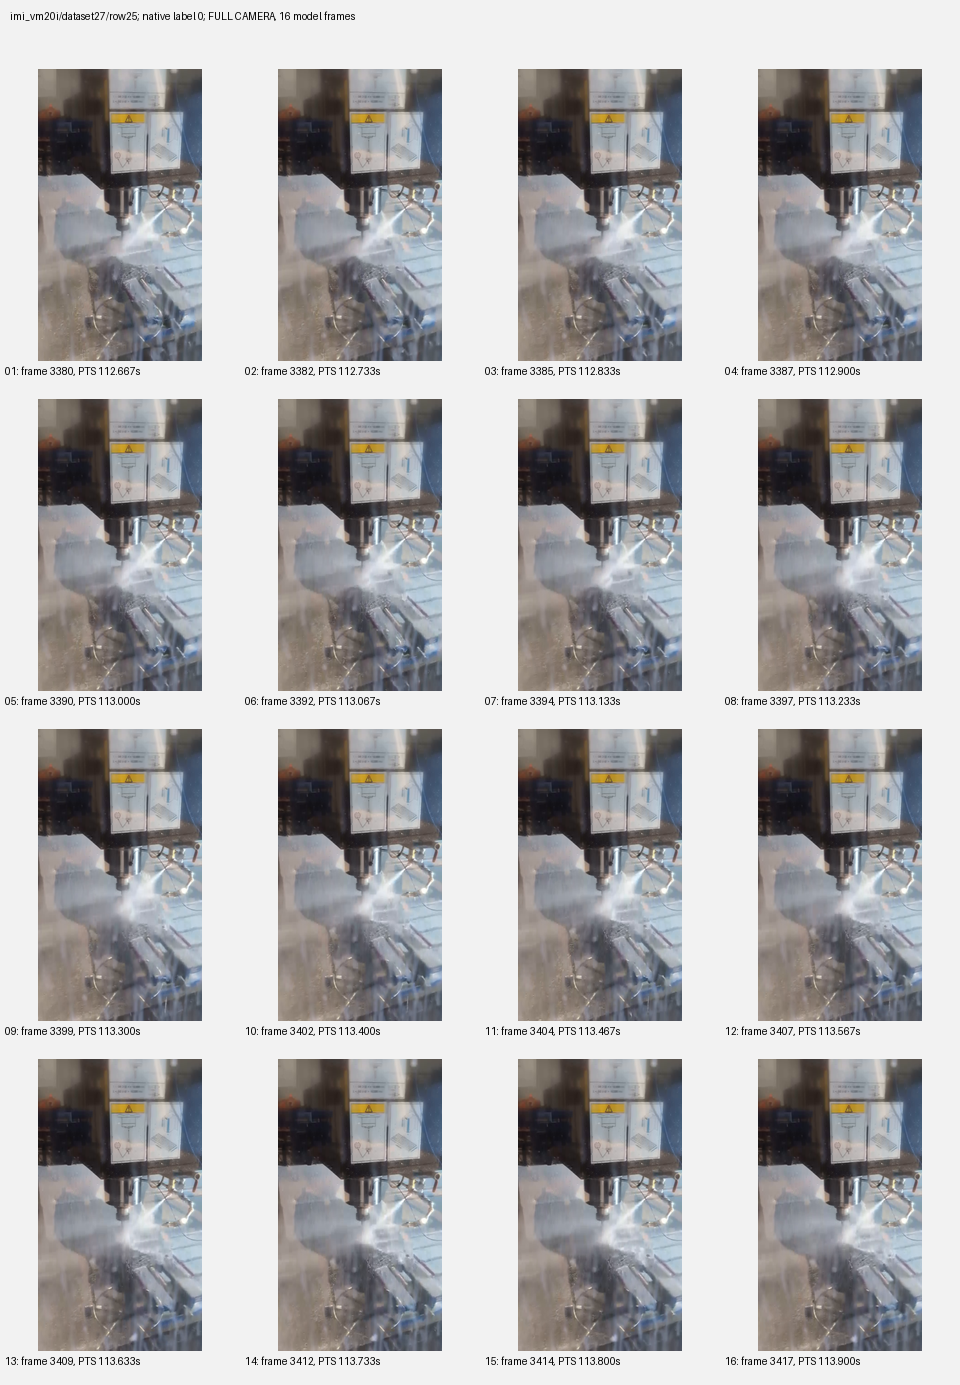
\includegraphics[width=\textwidth,height=.37\textheight,keepaspectratio]{figures/msm_example05_frames.png}\par\vspace{3mm}
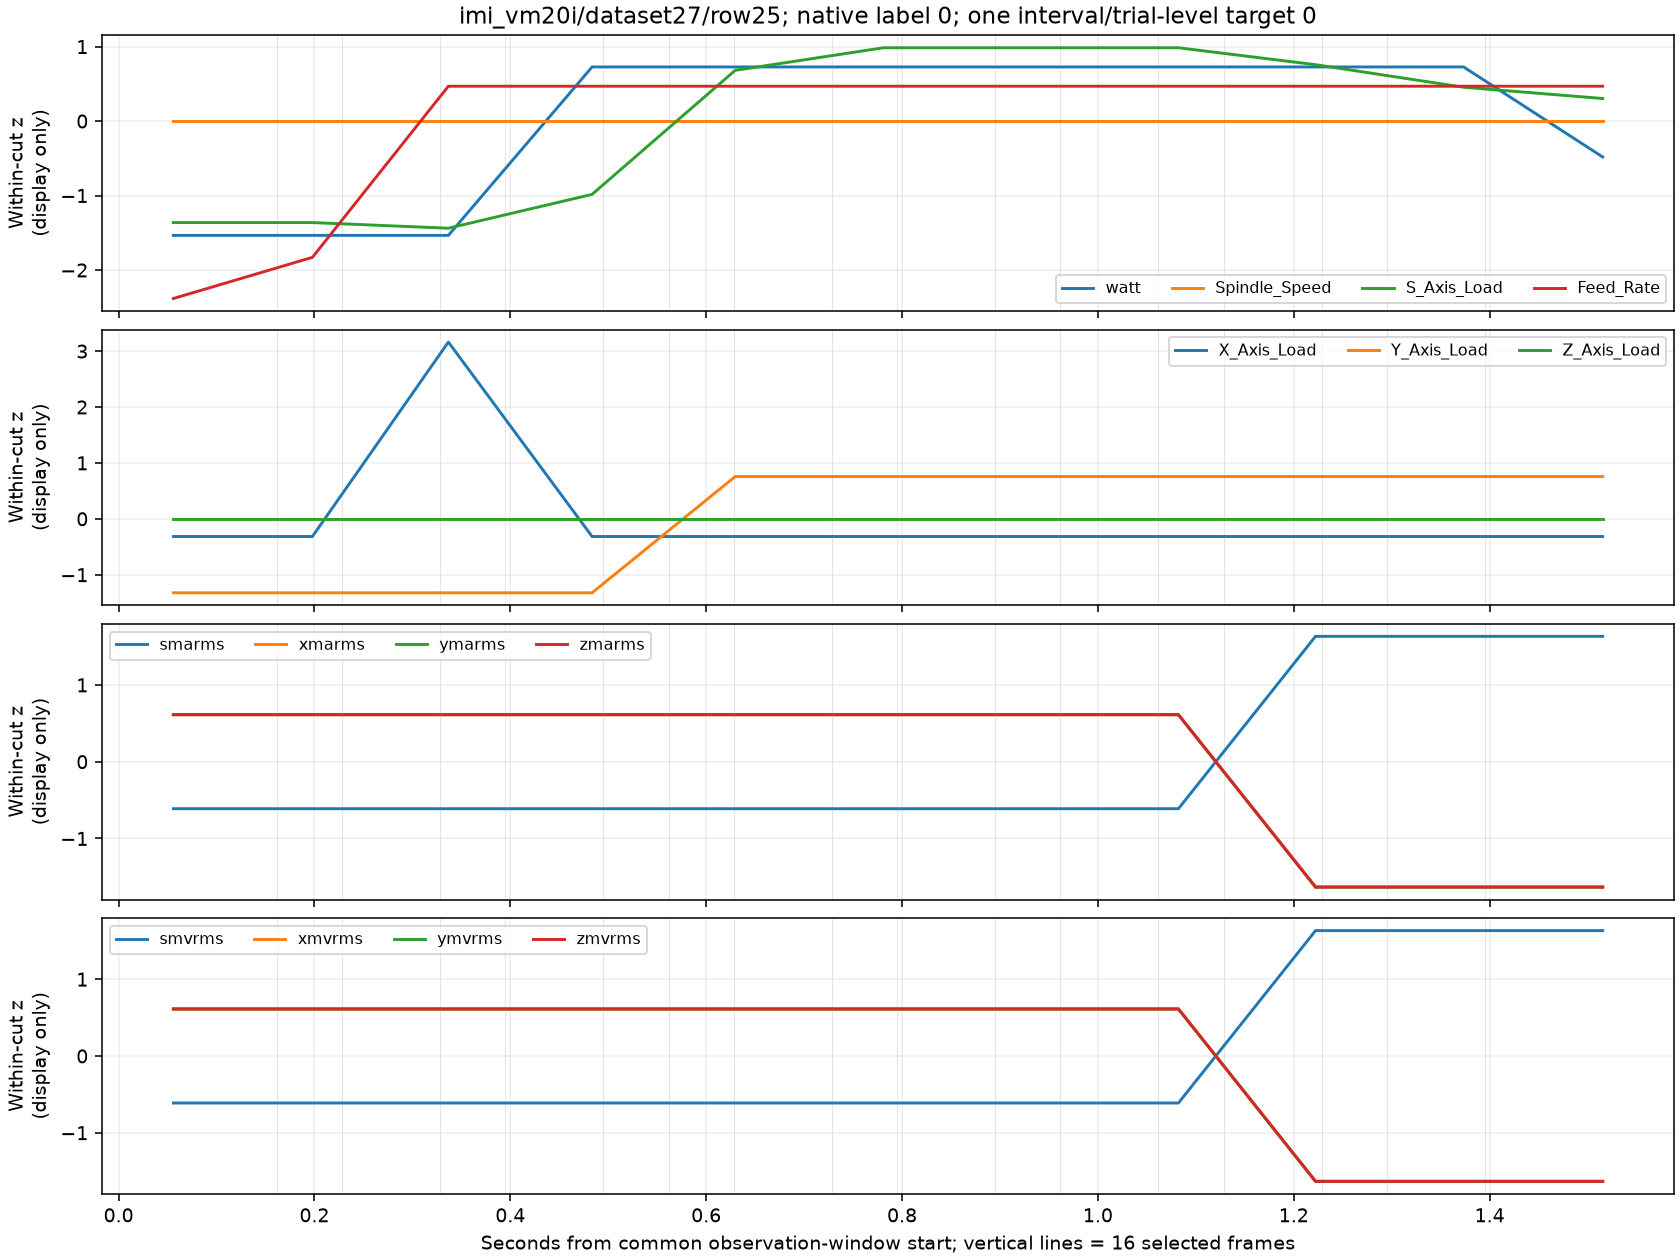
\includegraphics[width=\textwidth,height=.31\textheight,keepaspectratio]{figures/msm_example05_sensor.png}
\displaynote{The 16 frames and time-aligned MTConnect traces cover interval
\texttt{imi\_vm20i/dataset27/row25}, pair P03, at 112.405--113.941~s. The recorded label
is 0 (stable normal). Within-interval $z$ scores scale these curves for display. The
fitted model used training-only normalization and assigned one prediction to the whole
interval.}
\end{figure}
\ev{Illustrative input and identity source}{\EvidenceRef{E071}{}, \EvidenceRef{E072}{},
\EvidenceRef{E073}{data row 5}}
\section{Architecture Reuse, Adaptations, and Evaluation Protocol}
The pretrained condition (P) used the ResNet18-vd CNN backbone inside the RT-DETR-R18vd
checkpoint \citep{Zhao2024RTDETR}. The extractor stopped at the CNN feature maps, before
the hybrid Transformer encoder, detection decoder, and box heads. Spatial means from the
last three maps yielded 896 features per frame. Averaging across sixteen frames gave one
vector per cutting interval. With the backbone frozen, a newly fitted
$896\rightarrow128\rightarrow1$ head with ReLU and dropout~0.1 supplied the target
prediction. It had 114,945 trainable parameters.

The numerical branch is a fresh balanced L2 logistic regression on the ninety
statistics, with $C=1$. A separately fitted histogram gradient boosting model provides
the stronger sensor control. It is essential to keep that control separate: F2 consumes
the logistic branch, not the HGB predictions. Averaging combines the two branch
probabilities without a fitted fusion parameter. Original F2 is a newly fitted
unweighted L2 logistic model on visual and sensor probabilities generated out of fold.
No source failure head, scaler, calibrator or fusion coefficient is transferred.\ev{MSM
executed composition}{\EvidenceRef{E077}{}}

The clean and augmented quality gates are additional comparisons. They reuse a small
softmax gate over branch logits, with label-free image-quality summaries, numerical
variability, missing-channel fractions and availability flags. These summaries may
encode process context as well as degradation. A changing allocation therefore is not a
calibrated estimate of modality reliability. This matters because a reliability-aware
fusion argument requires a quality proxy that actually predicts error, rather than a
proxy that merely changes with the input \citep{Zhang2023QMF}. QG-clean uses clean OOF
views. QG-aug sees clean views plus seven predefined lowest-severity corruptions, while
F2-aug is the exposure-matched static control. Clean fitting, corruption exposure and
quality conditioning remain separate interventions.

R denotes a different question: initialization from a specifically completed
REASSEMBLE-learned CNN. The exact canonical source required by MSM's gate was
unavailable in the inspected evaluation, so that condition remains unmeasured. This does
not contradict the P completion or the later, differently specified ViFailback donor
study. Architecture reuse, generic pretraining and transfer of task-learned weights
retain separate provenance.

\subsection{Implementation Checks and Bounded Development Run}
The bounded development exercise was an engineering check: its two-epoch,
at-most-24-interval design restricted head updates and CNN frame forwards and prohibited
outer-assessment predictions. It could expose shape, gradient, memory or reload errors,
but could not estimate generalization. Generalization was assessed in the subsequent
evaluation on held-out intervals.

The saved implementation audit checks planned cases, source identities, native
assessment units, model budgets and checkpoint reloads. It also refits the fixed F2
estimator from saved clean OOF probabilities and reports zero coefficient discrepancy.
The CNN cache check reports maximum difference zero on an outer-training-only example.
These support consistency of the saved procedure and its outputs. Their scope is
narrower than reproduction of stochastic training: exact reload and metric recomputation
cannot alone certify that every training step would recur in another environment.\ev{MSM
implementation and reproduction scope}{\EvidenceRef{E078}{}}

\subsection{Evaluation Protocol and Conditions Without Estimates}
The completed matrix uses three outer and two inner StratifiedGroupKFold partitions,
fixed split seeds and training seeds 42, 123 and 20261023. Inner fits produce branch OOF
probabilities for learned fusion; outer assessments remain excluded from fitting. The
six target/grouping protocols yield 54 completed case records. The 54 cases include
different folds and seeds from overlapping protocols.

The main visual head runs for ten fixed epochs and the gate for forty. The assessment
uses a fixed threshold of 0.5, with no assessment-selected epoch or fitted primary
calibrator. The definitions in Section~\ref{sec:ch4-metrics} apply: AP is average precision,
not trapezoidal PR area, and F2 names the stacker. Each seed's disjoint outer predictions
are pooled before AP is computed; the three seed-specific APs are then summarized.
These are not mean-fold APs.

Conditions with a missing source checkpoint, inadequate class support or insufficient
temporal coverage yielded no estimate. The results below cover the conditions that met
the original criteria.\ev{MSM fixed evaluation protocol}{\EvidenceRef{E070}{}}

\section{Investigation A: Clean Unimodal and Fusion Comparison}
\label{sec:msm-clean}
On intact inputs, F2 had lower AP than its logistic sensor component at all three seeds.
The mean paired difference was $-0.0717$ (Table~\ref{tab:msm-clean}). F2 ranked
abnormal intervals more accurately than the visual branch or equal averaging. Sensor HGB
had the highest mean AP of the models compared.

\begin{table}[htbp]
\caption{MSM Prediction Performance With Intact Inputs}\label{tab:msm-clean}
\centering\small

\begin{tabular}{lrr}\hline Model&Mean AP&Seed SD\\\hline
Visual&0.2989&0.0109\\
Sensor logistic&0.8286&0.0000\\
Sensor HGB&0.9013&0.0000\\
Averaging&0.7356&0.0159\\
F2&0.7569&0.0111\\
F2-aug&0.7602&0.0098\\
QG-clean&0.8374&0.0134\\
QG-aug&0.8265&0.0162\\\hline
\end{tabular}
\displaynote{Entries summarize pooled average precision across three fixed seeds as the
mean and sample standard deviation.}
\end{table}
\ev{MSM primary results}{\EvidenceRef{E076}{}}

The visual training diagnostic averaged AP 0.9807 across the nine outer fits
(three folds by three seeds; range 0.9634--0.9994), compared with mean seed-specific
pooled held-out AP 0.2989. The training score is an in-sample mean on overlapping training
sets, not a second pooled assessment score. These predictions did not enter F2.
The gap is consistent with overfitting or acquisition shift, but does not isolate
visibility, alignment or representation quality as its cause.\ev{Visual training and
held-out diagnostics}{\EvidenceRef{E137}{}}

\section{Investigation B: Target-Definition and Grouping Sensitivities}
Logistic sensing had higher mean AP than F2 in all six prespecified protocols. Excluding
label~2 and grouping by calendar date gave 0.5218 for F2 and 0.8917 for logistic
sensing. That sensitivity analysis changes the target. Under the primary definition,
pooled prevalence was $336/1{,}895=0.1773$ and outer-fold prevalences ranged from
approximately 0.051 to 0.277. The fold-specific training-prior baseline had pooled AP
0.1454 because the fitted prior could vary across folds.


\begin{table}[htbp]
\caption{MSM Clean Performance Across All Six Protocols}\label{tab:msm-sensitivity}
\centering\small
\setlength{\tabcolsep}{4pt}
\begin{tabular}{lrrrrr}\toprule
Target and grouping & Vision & Sensor LR & HGB & F2 & QG-clean\\\midrule
Primary, experiment & 0.2989 & 0.8286 & 0.9013 & 0.7569 & 0.8374\\
Primary, machine/date & 0.5359 & 0.8922 & 0.8250 & 0.7389 & 0.8715\\
Primary, calendar date & 0.5444 & 0.8859 & 0.8386 & 0.8196 & 0.8521\\
Exclude 2, experiment & 0.3164 & 0.9403 & 0.8965 & 0.8235 & 0.9308\\
Exclude 2, machine/date & 0.3396 & 0.9265 & 0.9098 & 0.8562 & 0.7372\\
Exclude 2, calendar date & 0.4009 & 0.8917 & 0.9062 & 0.5218 & 0.6757\\
\bottomrule\end{tabular}
\displaynote{Mean of three seed-specific pooled abnormal-cutting APs. Primary protocols
use 1,895 intervals; label-2 exclusion leaves 1,770. All retain 336 positives.
Protocols reuse observations and change the fitting/assessment groups; they are
sensitivity analyses, not independent replications.}
\end{table}
\ev{All-protocol saved results}{\EvidenceRef{E135}{}, \EvidenceRef{E081}{}}

The sensor-reference ranking also depends on the protocol: logistic sensing has higher
mean AP than HGB in four of the six comparisons, while HGB leads in the primary
experiment-grouped comparison. The stronger sensor model is therefore not the same
across all target definitions and grouping choices.

For the primary experiment-grouped protocol, the mean F2-minus-logistic AP difference
of $-0.0717$ has a paired 95\% bootstrap interval of $[-0.1605,+0.0031]$ when
resampling 45 experiment folders, and $[-0.1004,-0.0515]$ when resampling five calendar
dates. These intervals use the same held-out predictions with different resampling
units. The folder interval includes zero; the date interval is wholly negative. Across
the six protocols, all observed mean differences favor logistic sensing, and five of
the six folder-bootstrap intervals exclude zero. Both bootstrap schemes hold fits and
split assignments fixed and cannot account for unidentified equipment reuse.

QG-clean averaged $0.0088$ AP above logistic sensing, with one negative seed and a
calendar-date bootstrap interval of $[-0.0971,0.0564]$. The interval admits gains and
losses and leaves equivalence unresolved.\ev{Milling results and paired bootstrap
units}{\EvidenceRef{E081}{}, \EvidenceRef{E144}{}}

\section{Investigation C: Input Degradation, Quality Gates, and Fallback}
Table~\ref{tab:msm-robustness} covers the strongest declared severity of all seven
corruption families. F2-aug and QG-aug have matched augmentation exposure; this control
separates quality conditioning from additional corruption training.

At the highest sensor-noise level, QG-aug reached 0.2986 mean AP, close to intact
vision at 0.2989. F2 reached 0.2069 and noisy sensor HGB reached 0.6062. Under the
strongest image blur, QG-aug achieved 0.6828, below F2 at 0.7714 and intact logistic
sensing at 0.8286. The comparison therefore depends on which stream deteriorates and
which predictor remains available. The tests also covered brightness and contrast
changes, occlusion, frame omission, zeroed channels and explicitly missing channels.


\begin{table}[htbp]
\caption{MSM High-Severity Corruption and Known Absence}\label{tab:msm-robustness}
\centering\small\setlength{\tabcolsep}{4pt}
\begin{tabular}{lrrrrr}\toprule
Condition & Intact & F2 & F2-aug & QG-aug & HGB\\\midrule
Blur ($\sigma=4$) & 0.8286 & 0.7714 & 0.7712 & 0.6828 & 0.9013\\
Brightness/contrast (0.2) & 0.8286 & 0.7700 & 0.7688 & 0.6787 & 0.9013\\
Occlusion (40\%) & 0.8286 & 0.7708 & 0.7709 & 0.8332 & 0.9013\\
Frame omission (12/16) & 0.8286 & 0.7604 & 0.7654 & 0.8331 & 0.9013\\
Sensor noise ($1\,\mathrm{SD}$) & 0.2989 & 0.2069 & 0.2062 & 0.2986 & 0.6062\\
Zeroed channels (50\%) & 0.2989 & 0.4198 & 0.4188 & 0.4754 & 0.6466\\
Missing channels (50\%) & 0.2989 & 0.4477 & 0.4469 & 0.5115 & 0.5460\\
Vision absent & 0.8286 & 0.8286 & 0.8286 & 0.8286 & 0.9013\\
Sensors absent & 0.2989 & 0.2989 & 0.2989 & 0.2989 & --\\
\bottomrule\end{tabular}
\displaynote{Mean seed-specific pooled AP on the primary cohort. Intact denotes
logistic sensing for visual faults and vision for sensor faults. HGB receives the
same sensor condition; it is unavailable when all sensors are absent. Known absence
uses the programmed survivor route. Intermediate severities remain in the saved
robustness report (E080).}
\end{table}
\ev{All seven stress families}{\EvidenceRef{E136}{}, \EvidenceRef{E080}{}}

Whole-modality absence invokes a separately programmed surviving-branch fallback:
0.8286 AP without vision and 0.2989 without sensors. Equal fallback scores across
fusion methods are imposed behavior, not adaptive recovery learned from data.
Differences in augmentation exposure between a gate and its static control would
confound the effect of quality conditioning.\ev{MSM input perturbation and fallback
results}{\EvidenceRef{E080}{}}

\section{Metric Trade-offs, Limitations, and Transition to ViFailback}
For seed~42, F2 had lower AP than logistic sensing but a lower Brier score (0.0561
versus 0.0617) and higher F1 score (0.8204 versus 0.8113). QG-clean had higher AP than
F2, a worse Brier score of 0.0644 and a lower F1 score of 0.7864. Thus the ranking
comparison favored logistic sensing, whereas probability error and fixed-threshold
decisions favored F2 for this seed. The relative performance of the gates depended on
the input condition.

The logistic sensor model uses balanced class weights and no fitted primary calibrator,
whereas F2 is unweighted and fits an intercept and two coefficients to group-OOF branch
probabilities. These different fitting objectives and probability mappings can affect
probability error and ranking differently. They offer a plausible explanation for the
AP--Brier trade-off, but this comparison does not isolate class weighting, the added
visual input or the fitted mapping as its cause.\ev{MSM seed-42 scores and fitting
definitions}{\EvidenceRef{E136}{}, \EvidenceRef{E068}{}, \EvidenceRef{E149}{},
\EvidenceRef{E150}{}}

The visual model ranked held-out intervals poorly despite a much stronger training
result. Inadequate features, limited event visibility, residual alignment error and
experiment-specific appearance could each contribute. Independent annotations of event
visibility and a matched representation comparison on the same groups would help
distinguish these explanations.

MSM therefore supplies a completed external comparison of representations, fusion,
target/grouping sensitivity and controlled robustness. Its unavailable R condition
leaves learned-weight transfer unanswered. Chapter~\ref{ch:vifailback} addresses that
separate question with a specified REASSEMBLE donor and task-disjoint robotic episodes,
while retaining its narrower adaptation coverage and unexecuted corruption study.

\chapter{ViFailback Case Study: Task-Disjoint Evaluation and Representation Transfer}
\label{ch:vifailback}

ViFailback extends the robotic studies to complete episodes on held-out manipulation
tasks and to learned-representation transfer from REASSEMBLE. The completed frozen and
donor comparisons favored logistic sensing over F2, while donor effects varied across
target seeds. Target-CNN adaptation has only bounded single-fold evidence, with
inconclusive matched effects. The study contributes clean-input representation, fusion
and metric analyses; its planned corruption evaluation was not executed.

\section{Motivation and Comparison Scope}
Three cameras and robot observations provide a different test of the relation between
visual representations and completed manipulation outcomes \citep{Zeng2026ViFailback}.
The study asks whether the original fusion procedure adds value on task-disjoint
episodes, and whether a REASSEMBLE-learned CNN helps after fitting a new target head.

The primary replication contrasts original frozen vision, logistic sensing, averaging
and F2. HGB supplied a stronger numerical reference, while camera ablations and donor
transfer tested visual representations. The 30 October 2026 priority note reframed the primary comparison after frozen-branch
outer predictions were available; it explicitly describes a reporting clarification,
not prospective preregistration. The 29 October report snapshot already contained
original frozen three-view and high-camera results, logistic/HGB sensor references,
averaging, F2 and clean gate comparisons. Thus the weak visual ranking and the original
fusion-versus-sensor direction were available before this clarification. The exact
sequence of human inspection is not independently established. The note retained the
cohort, splits, recipes and budgets; it did not create a fresh confirmatory holdout.\ev{Dated
priority clarification and preceding snapshot}{\EvidenceRef{E142}{}, \EvidenceRef{E143}{}}

All reported comparisons concern intact inputs. Table~\ref{tab:vif-status} distinguishes
the complete frozen/donor comparisons from target-CNN adaptation on one outer fold and
the separate hundred-epoch pilots.\ev{Comparison scope}{\EvidenceRef{E102}{},
\EvidenceRef{E096}{}, \EvidenceRef{E115}{}, \EvidenceRef{E116}{}}

\section{Dataset, Episode Labels, and Cohort Construction}
The native source contains 5,202 episodes with 4,545 failure and 657 no-failure
annotations across 100 canonical tasks and 109 source directories. The evaluation pins
both the original release and its converted LeRobot representation
\citep{ViFailbackHF2025}. Matching version identities matters because the paper, source
directory layout, converted observations and admitted model cohort describe different
levels of the evidence.

The source paper evaluates visual-symbol and visual-language reasoning, including
open-ended failure explanations and policy interventions. Its model does not consume the
280 engineered robot-observation features used here. Its benchmark also differs in task,
cohort and metric: a reported visual-language benchmark score is not failure-positive or
both-class AP for this classifier. The paper therefore provides dataset and
completed-outcome context, rather than a directly comparable fusion score.

The final cohort contains 4,382 episodes, including 3,753 failures and 629 successes
across 99 canonical tasks. Failure is the positive class, giving prevalence 0.856458. An
episode contributes one target, although it supplies 48 sampled RGB images. The task is
retrospective prediction of native whole-episode annotations. It is not frame-level
failure localization, verification of a task's final mechanical success independently of
annotation, or advance warning before a failure occurs.\ev{Native and final ViFailback
labels}{\EvidenceRef{E087}{}}

\subsection{Exclusions and Independence Limits}
The provisional core contained 4,384 episodes after 818 unique exclusions or
quarantines. Full three-camera quality checks then identified two defective camera
streams: episode~2071's right wrist and episode~4784's left wrist. Their source bytes
remain preserved. Removing them from analysis produces the final 4,382 common-support
episodes and 820 unique exclusions. Reason counts can overlap; summing them as if
disjoint would overstate the excluded population.

The records distinguish exact trajectory/video duplication and invalid telemetry from
low visual quality and uncertain semantics. Duplication and invalid observations can
invalidate the input contract; visual difficulty does not justify excluding examples
after inspecting correctness. Coordinate task~55 remains quarantined rather than
receiving a guessed sign correction. Agreement of converted 25~Hz observations does not
independently certify original hardware synchronization. Canonical task separation also
leaves operator/session identity and semantic similarity between tasks unresolved,
limiting the independence claim to the grouping actually checked.\ev{Cohort validity and
remaining dependence}{\EvidenceRef{E093}{}}

\section{Preparation, Three-View Inputs, and Pre-Checks}
Sixteen uniform, matching frame indices are selected in each of three cameras. These are
sixteen temporal positions and 48 images, not 48 distinct timestamps. The image
processor follows the shared RGB preprocessing specified in
Appendix~\ref{app:implementation}, Section~\ref{sec:rtdetr-preprocessing}.
Equal camera and temporal means remove order information from
the episode embedding. A fixed crop shown in an example is context visualization, not a
detected object or validated failure location.

The sensor adapter retains fourteen position, twelve nonplaceholder velocity and two
gripper-effort fields. Ten statistics per channel produce 280 values. These observations
are not calibrated wrench or force/torque measurements. Labels, failure categories,
action commands, keyframes and task/source identifiers do not enter ordinary model
features. Per-episode feature calculation is separated from population fitting:
standardizers use T only, and calibration uses disjoint C examples.

The twenty-example visual pilot was selected for observability and balance. Nineteen
decided observations agreed with native labels; B02 remained uncertain. This is a
bounded project examination, not an independent human-rated prevalence sample or a
held-out classifier benchmark. The additional automated consistency checks are also not
a signed second-human review. Technical decoding and a successful native-label join do
not resolve every episode's semantic meaning.\ev{ViFailback
preprocessing}{\EvidenceRef{E088}{}}\ev{Scope of independent
checks}{\EvidenceRef{E092}{}}

\section{Models, Transfer/Adaptation Regimes, and Evaluation Protocol}
The original visual branch loaded the ResNet18-vd CNN backbone inside the pretrained
RT-DETR-R18vd checkpoint \citep{Zhao2024RTDETR}. The extractor stopped at the CNN
feature maps, before the hybrid Transformer encoder, detection decoder, and box heads.
Spatial means of three maps with 128, 256, and 512 channels yielded 896 features per
image. The branch averaged these features across frames and cameras and fitted a new
$896\rightarrow128\rightarrow1$ head to predict the episode outcome. Three-view pooling,
the sensor statistics, and the task partitions were specific to ViFailback.

The logistic sensor branch uses balanced L2 regression with $C=1$, training-only scaling
and a separately fitted sigmoid calibrator. Averaging and F2 consume its calibrated
probabilities alongside the visual branch. F2 is unweighted L2 logistic probability
stacking; HGB is a stronger separate reference and never replaces the sensor input
inside original F2. Consequently, a gain over vision or logistic sensing cannot be
reported as a gain over the strongest available unimodal method.

HGB uses 200 iterations, learning rate 0.05, L2 penalty 0.1 and minimum leaf size
twenty; leaves 7, 15 and 31 are selected on V macro AP, followed by C-only calibration.
Its search is real candidate selection, unlike the fixed MSM recipe or a claim that
every parameter was optimized. It remains secondary and does not change the prespecified
F2 input after its favorable assessment.

\ev{Exploratory HGB recipe}{\EvidenceRef{E094}{}}

The donor arms transferred compatible CNN tensors from a completed source checkpoint and
fitted a fresh ViFailback head, scaler, calibrator and fusion model. The FROZEN and
DONOR conditions held the CNN weights fixed. The FULL conditions train the executed CNN
convolutions and normalization affine terms while holding running moments fixed; their
completed coverage is stated below. This is CNN adaptation, not training the detector
encoder, decoder or detection heads. The completed DONOR comparison therefore measures
supervised target-head fitting on a transferred frozen representation.\ev{Matched model
definitions}{\EvidenceRef{E097}{}}

\subsection{Task Partitions, Calibration, and Fitting Budgets}
The original protocol uses three outer task-disjoint folds and three inner OOF
assessments within each outer-training pool. Each branch separates gradient-fitting T,
checkpoint-selection V, calibration C and assessment A task groups. After excluding the
assessment tasks, the remaining task groups are allocated approximately 60\% to T,
20\% to V and 20\% to C, with rounding by task count. These are task-group proportions,
not episode proportions. A final branch is not automatically fitted to the entire
outer-training pool: its T/V/C roles remain distinct. The inner assessment probabilities
build a meta bank without using examples that fitted, selected or calibrated their
generating branch.

Checkpoint selection uses validation macro AP; the selected checkpoint is then
calibrated on C, and assessment uses a fixed threshold of 0.5. Failure AP, success AP
and their arithmetic mean are retained. With failure prevalence above 85\%,
failure-positive AP alone can conceal poor success discrimination. Pooled AP is
calculated from disjoint outer predictions, separately for each seed. It is not the
arithmetic mean of fold APs, and seed repetition does not add independent episodes.

The later matched twenty-epoch arms use the first twenty epochs of a fixed cosine-50
schedule, while the hundred-epoch arms use cosine-100. Highest V macro AP selects the
checkpoint, then lower V BCE and the earliest epoch resolve ties. All configured epochs
are intended to execute even when the chosen checkpoint is earlier. The twenty-epoch
study has a complete three-inner OOF bank. The hundred-epoch pilot instead reserves 788
meta episodes under one predeclared role, followed by 1,107 outer assessments. It is not
a full nested three-fold hundred-epoch experiment.\ev{Original evaluation
contract}{\EvidenceRef{E094}{}}\ev{Matched training contract}{\EvidenceRef{E098}{}}

\section{Empirical Investigations}
The original study evaluated the frozen visual branch, its high-camera control, sensor
models and clean fusion. Table~\ref{tab:vif-status} records the coverage of the matched
comparisons. Conditions and seeds reuse episodes; the hundred-epoch pilots use a separate
fitting protocol from the twenty-epoch nested comparison.\ev{Matched evaluation scope}{\EvidenceRef{E115}{},
\EvidenceRef{E116}{}}

\begin{table}[htbp]
\caption{Final Scope of the Matched ViFailback Comparisons and Robustness
Tests}\label{tab:vif-status}
\centering\small

\begin{tabularx}{\linewidth}{@{}lX@{}}\toprule
Condition & Evaluation coverage\\\midrule
\multicolumn{2}{@{}l}{\textit{Completed final scope}}\\
Completed fits & 79 of 111 planned fits\\
FROZEN20 & 36 fits across three seeds and three outer folds\\
DONOR20 & 36 fits across three seeds and three outer folds\\
FULL20 & Four fits: seed 42, outer fold 0 and its three inner fits\\
FROZEN100 / FULL100 / DONOR100 & One single-role pilot fit each\\\addlinespace
\multicolumn{2}{@{}l}{\textit{Conditions without assessment results}}\\
Remaining FULL20 & 32 planned fits not executed\\
SQ3 corruption tests & Missing, degraded and temporally shifted inputs\\\bottomrule
\end{tabularx}
\displaynote{The completed fits support 22 outer fusion assessments: eighteen
frozen/donor twenty-epoch assessments, one FULL20 assessment and three pilots. Completed
fits and inconclusive contrasts are distinct from unexecuted conditions. All completed
comparisons used intact inputs.}
\end{table}
\ev{Matched fit coverage recorded on 24 November 2026}{\EvidenceRef{E115}{}, \EvidenceRef{E116}{}}

\subsection{Unimodal References and Original Fusion}
The original frozen visual head completed all 36 planned fits, as did its
high-camera-only control. The logistic sensor branch is deterministic under the fixed
partitions. S1 and S3 denote the same fitted recipe. HGB supplies a stronger numerical
comparison. Table~\ref{tab:vif-bothclass} gives the pooled seed-42 scores from the
thesis experiment. Reporting average precision for each outcome makes the disparity
between failure and success ranking visible.

\begin{table}[htbp]
\caption{ViFailback Prediction Performance by Outcome Class}\label{tab:vif-bothclass}
\centering\small

\begin{tabular}{lrrrr}\hline Model&Failure AP&Success AP&Macro AP&AUROC\\\hline
Frozen visual V1&0.853052&0.137260&0.495156&0.479402\\
Logistic sensor&0.954370&0.343577&0.648974&0.784370\\
Sensor HGB&0.970510&0.429530&0.700020&0.853756\\
Equal averaging (F1)&0.931760&0.289037&0.610399&0.716501\\
Original F2&0.945168&0.312405&0.628787&0.752701\\\hline
\end{tabular}
\displaynote{Scores pool the original seed-42 results separately for each class.}
\end{table}
\ev{Original both-class scores}{\EvidenceRef{E089}{}}

\begin{table}[htbp]
\caption{Completed Original ViFailback Controls}\label{tab:vif-controls}
\centering\small
\begin{tabular}{lrrr}\toprule
Model & Seed 42 & Seed 123 & Seed 20261023\\\midrule
Three-view V1 & 0.4952 & 0.4964 & 0.4844\\
High-camera control & 0.4908 & 0.4915 & 0.4915\\
Clean quality gate & 0.6340 & 0.6363 & 0.6359\\
Availability-only gate & 0.6375 & 0.6431 & 0.6397\\
Logistic sensor & 0.6490 & 0.6490 & 0.6490\\
\bottomrule\end{tabular}
\displaynote{Reported both-class macro AP, pooling all 4,382 outer-held-out episodes
per seed under the original study. The high-camera head completed 36 fits, as did
three-view V1. The two gates use intact inputs; these scores do not test corruption
adaptation.}
\end{table}
\ev{Original controls}{\EvidenceRef{E089}{}, \EvidenceRef{E090}{}}
The high-camera control did not consistently improve on three-view pooling. The clean
quality gate scored below its availability-only control and logistic sensing at each
seed (Table~\ref{tab:vif-controls}); these point comparisons do not establish a
reliability mechanism or statistical equivalence.

The completed target-CNN comparisons are assessed against their matched frozen controls
below. Their existence does not imply completion of the three-fold, three-seed
adaptation matrix.

\paragraph{Original fusion comparison.}
In the original frozen comparison, F2 improves over vision and averaging but has lower
pooled macro AP than the logistic sensor branch for all three seeds: 0.628787, 0.625400
and 0.621067 against 0.648974. The sensor HGB point score is higher still. These results
support a narrower conclusion than ``fusion works'': the numerical information can
improve weak visual prediction, but adding the visual branch does not improve the
strongest component used in F2.

\subsection{Matched Frozen Versus REASSEMBLE-Donor Transfer}
The later matched twenty-epoch comparison also favored the numerical reference.
Table~\ref{tab:vif-matched} lists every seed's pooled score after all three outer
assessments complete. Despite small fold-specific differences around logistic sensing,
FROZEN20's pooled F2 scores are lower by 0.019694, 0.021935 and 0.024419. Saved
conditional task-cluster intervals for these differences exclude zero. This is a
model-and-protocol-specific negative comparison, not proof that every visual
representation will damage fusion.

\begin{table}[htbp]
\caption{ViFailback Performance in the Matched Comparison}\label{tab:vif-matched}
\centering\small

\begin{tabular}{lrrrr}\hline Arm&Seed&Visual&F2&Sensor LR\\\hline
FROZEN20&42&0.507865&0.629280&0.648974\\
FROZEN20&123&0.495229&0.627039&0.648974\\
FROZEN20&20261023&0.487612&0.624555&0.648974\\
DONOR20&42&0.491368&0.627750&0.648974\\
DONOR20&123&0.489011&0.637852&0.648974\\
DONOR20&20261023&0.492185&0.630936&0.648974\\\hline
\end{tabular}
\displaynote{Macro average precision was calculated from pooled predictions over three outer folds.}
\end{table}
\ev{Matched complete outer comparisons}{\EvidenceRef{E096}{}}

\paragraph{Transferred parameters and paired contrasts.}
Following donor feature extraction, DONOR20 completed 36 target-head fits. Its source
completed 100 epochs and selected epoch~47; 115 compatible CNN tensors are loaded,
without source head, scaler, calibrator or F2 coefficients. This establishes an executed
learned-representation transfer experiment with fresh target supervision. The fixed
donor is one source-training realization; three target seeds do not replicate donor
selection or training.

It does not establish a consistent predictive advantage. Relative to FROZEN20, donor
visual pooled macro-AP differences are $-0.016497$, $-0.006219$ and $+0.004573$. Their
saved task-cluster intervals cross zero. Donor F2 differences are mixed: $-0.001530$,
$+0.010813$ and $+0.006381$. F2 with the transferred encoder achieved higher macro-AP
than F2 with the frozen encoder for two of the three target seeds. The sensor-only
logistic model achieved higher macro-AP than the transferred-encoder F2 model for all
three seeds.

On the same 1,107 outer episodes, the hundred-epoch frozen-backbone pilot achieved macro
AP of 0.550995 for vision and 0.694219 for F2. This arm reused the completed historical
head-training trajectory after verifying the same checkpoint selection. The
donor-backbone pilot achieved 0.571448 and 0.696600, respectively. Both pilots used a
single seed and fit role, with a separate 788-episode bank for fitting fusion. Neither
pilot updated the target CNN.\ev{Donor identity and pilot fit
provenance}{\EvidenceRef{E098}{}, \EvidenceRef{E099}{}, \EvidenceRef{E100}{}}

\subsection{Partial Target-CNN Adaptation}
On the same 1,107 outer-fold-0 episodes, FULL20 achieved visual macro AP .492370 and F2
.697858; FULL100 achieved .544332 and .699260. The corresponding sensor LR and HGB
references were .707996 and .757878. Table~\ref{tab:vif-adaptation} reports the paired
differences against each arm's own frozen control. Neither visual nor F2 contrast
resolves improvement or deterioration; an interval including zero does not establish
equivalence. The twenty-epoch meta bank contains 3,275 inner-OOF episodes, whereas the
hundred-epoch pilot uses 788 held-out meta episodes. Comparisons between these protocols
cannot isolate training duration.

\begin{table}[htbp]
\caption{Completed ViFailback CNN-Adaptation Contrasts}\label{tab:vif-adaptation}
\centering\small
\begin{tabularx}{\linewidth}{@{}lYY@{}}\toprule
Contrast & Visual macro-AP difference & F2 macro-AP difference\\\midrule
FULL20 $-$ FROZEN20 & $+.004946$ [$-.027460$, $+.040927$] & $-.009260$ [$-.026854$, $+.005016$]\\
FULL100 $-$ FROZEN100 & $-.006662$ [$-.027982$, $+.027078$] & $+.005040$ [$-.019473$,
$+.029255$]\\\bottomrule
\end{tabularx}
\displaynote{Seed 42, outer fold 0 only. Paired 95\% intervals resample canonical tasks,
conditional on fixed models; they omit refitting, selection and unverified
session/operator dependence. Twenty- and hundred-epoch fusion-fitting protocols differ.}
\end{table}
\ev{Completed adaptation results and recorded independent arithmetic}{\EvidenceRef{E115}{}}

\subsection{Calibration, Threshold Behavior, and Corruption Limits}
In outer fold~0, FROZEN20 seed~42 F2 had macro AP 0.7071 and Brier score 0.1539,
yet balanced accuracy was 0.5 at threshold 0.5. Ranking and probability metrics thus
need not imply useful decisions at the fixed operating threshold; tuning it on these
assessment episodes would bias decision-performance estimates.\ev{Matched secondary
metrics}{\EvidenceRef{E154}{}, \EvidenceRef{E096}{}}

The retained source implements calibration as $p=\sigma(a s+b)$ on the branch's raw
failure logit $s$, with $a$ and $b$ fitted on C only. Under this convention a negative
$a$ reverses within-fit ranking. The saved matched-study report attributes negative
visual slopes to outer fold~0 in every FROZEN20 and DONOR20 seed, and to FULL20
seed~42. Table~\ref{tab:vif-calibration} gives those reported coefficients and paired
raw/calibrated visual macro APs. FROZEN20 and DONOR20 outer folds~1 and~2, and all
three hundred-epoch pilots, have positive reported slopes.

\begin{table}[htbp]
\caption{Reported ViFailback Visual Ranking Reversals in Outer Fold 0}
\label{tab:vif-calibration}\centering\small
\begin{tabular}{llrrr}\toprule
Arm & Seed & Slope $a$ & Raw macro AP & Calibrated macro AP\\\midrule
FROZEN20 & 42 & -0.0335 & 0.5179 & 0.4874\\
FROZEN20 & 123 & -0.0592 & 0.5332 & 0.4743\\
FROZEN20 & 20261023 & -0.0442 & 0.5228 & 0.4834\\
FULL20 & 42 & -0.1219 & 0.5133 & 0.4924\\
DONOR20 & 42 & -0.0567 & 0.5498 & 0.4632\\
DONOR20 & 123 & -0.0532 & 0.5395 & 0.4702\\
DONOR20 & 20261023 & -0.0641 & 0.5447 & 0.4664\\
\bottomrule\end{tabular}
\displaynote{The same 1,107 outer episodes per row; raw AP uses the uncalibrated
failure scores, not a new model fit. Values are retained report results. Individual
calibrator and keyed prediction files were unavailable in the inspected evidence. The
check verified the equation and correspondence with retained reports, without numerically
reconstructing each fitted map.}
\end{table}
\ev{Raw/calibrated ranking and F2 input definition}{\EvidenceRef{E139}{}}

The inspected training path saves calibrated \texttt{probability} values, and the F2
path consumes that column in both the inner meta bank and outer assessment. This is
consistent with the report that FROZEN20/DONOR20 F2 used calibrated visual inputs,
rather than raw-score controls; the missing per-fit artifacts prevent a new verification
of execution for every fit. The outer-fold report does not establish the signs of every
inner-fit or sensor calibrator. Negative visual slopes describe an inverse relationship
fitted on C; they do not identify whether weak representation, calibration-sample
variation or another mechanism caused it. With different maps across folds, even
positive slopes can alter pooled ordering. For example, FROZEN20 seed~42 pooled visual
macro AP was 0.5088 raw and 0.5079 calibrated; DONOR20 was 0.5166 and 0.4914.
These are descriptive diagnostics, not permission to revise calibration after observing
outer performance.

\paragraph{Unmeasured corruption performance.}
ViFailback contributes clean-input comparisons to SQ1 and SQ2. Performance under missing,
degraded or temporally shifted inputs was not measured. The specified visual interventions
included missing frames or windows, blur, occlusion, camera loss, JPEG degradation and
within-episode timing shifts. Sensor interventions included missing channels or
intervals, Gaussian noise, frozen readings and timing shifts. The matched CNN comparison
contained no quality gate. Performance under these interventions remains a question for
future work.

The specified availability rules route complete single-modality absence to the surviving
branch and abstain when both inputs are absent. These rules do not estimate reliability
from data. The edge-padded sampling shifts simulate timing errors without measuring
drift between hardware clocks.\ev{Specified corruption and fallback
conditions}{\EvidenceRef{E091}{}}


\section{Synthesis, Limitations, and Role in the Thesis}
The three donor-minus-frozen visual contrasts had task-cluster intervals spanning zero.
These paired intervals used 2,000 draws and held the fitted models, donor and split
assignments fixed. They omit uncertainty from refitting, donor selection and possible
dependence within sessions or operators. The exploratory comparisons had no multiplicity
adjustment. Coefficients were fixed before outer scoring, although the labels and some
tasks had already been examined during development.\ev{Task-cluster uncertainty and
evaluation limits}{\EvidenceRef{E101}{}}

The complete twenty-epoch frozen/donor comparison addresses representation transfer. The
inconclusive target-adaptation contrasts leave its consistency across task folds and
seeds unresolved. Performance under missing, degraded or temporally shifted inputs
remains unmeasured.

ViFailback adds held-out-task assessment and a completed learned-representation
transfer comparison to the earlier studies. It supplies the donor condition unavailable
in MSM, but does not replace MSM's completed corruption and sensitivity evidence.
The transferred CNN gave mixed effects across target seeds; the bounded adaptation
contrasts leave full-cohort adaptation unresolved. Chapter~\ref{ch:discussion} compares
the studies' implications, including HANDOVER's restricted learned-fusion eligibility.

\chapter{Integrated Discussion}
\label{ch:discussion}

The original proposal asked how process-aware multimodal architectures could be designed
and evaluated for robotic welding. PHM was already under way when Intel Welding was
re-examined. Intel Welding provided intended-condition categories, but independent
defect outcomes were unavailable and the proposed holdout had already appeared in a data
audit. REASSEMBLE subsequently supplied labelled completed actions, aligned observations
and recording identities for the central fusion comparison
(Appendix~\ref{app:chronology}).\ev{Original application and study chronology}
{\EvidenceRef{E002}{pp. 2--3}, \EvidenceRef{E118}{}}

REASSEMBLE provides the central controlled study; Table~\ref{tab:cross-study} places the
other evaluations around it. Comparisons use common targets and held-out observations
within each study. MSM refitted the predictors on milling data, HANDOVER evaluated its
unimodal models and equal averaging on the official split, and ViFailback additionally
tested transfer of REASSEMBLE-trained CNN weights. None is a zero-shot cross-dataset
test. Extending these findings to welding requires welds reserved for assessment and an
independently measured quality outcome.

\begin{table}[htbp]
\caption{Interpretation of the Results Within Each Study}\label{tab:cross-study}
\centering\small
\begin{tabularx}{\textwidth}{P{27mm}YYY}
\toprule Study and role & Target/unit & Supported lesson & Principal boundary\\\midrule
PHM --- proxy validity & Photographic proxy per gear run & Three sensor groups gave no
clear improvement over the training mean & Independent physical-damage reference
unavailable\\
REASSEMBLE --- central controlled study & Completed-action failure & Stacking improved
on sensors; advantage over averaging unresolved & Pooled attribution and exploratory
selection limit interpretation\\
MSM --- external manufacturing and corruption & Abnormal milling interval & Logistic
sensing ranked above stacking in all six protocols & Primary uncertainty depends on
resampling unit (Section~\ref{sec:discussion-fusion})\\
ViFailback --- task-disjoint transfer & Whole-episode outcome & Original stacking and
complete FROZEN20/\allowbreak DONOR20 stacking scored below logistic sensing on pooled macro AP &
One-fold adaptation inconclusive; corruption unmeasured\\
HANDOVER --- supporting official split & Handover success/failure & Averaging fell
below logistic sensing & Participant grouping required for learned fusion
unavailable\\\bottomrule
\end{tabularx}
\displaynote{Each effect applies to the evaluation protocol for its study.}
\end{table}

\section{Representation Suitability --- Answer to SQ1}
In PHM, the image-regression experiment extracted detector features during a full
prediction pass. In the principal sensor experiment, post-run photographs instead
supplied the continuous target. A patch-based Transformer encoded sequences summarising
speed, torque, temperature, vibration and condition indicators. For SQ1, the regression
error measures how well this representation predicts the photographic proxy. Assessing
physical tooth damage would require a separate reference (Chapter~\ref{ch:phm}).

Across 4,530 completed REASSEMBLE actions, sensor statistics achieved pooled failure AP
0.429, against 0.242 for the initial scratch-trained PatchTST and 0.231 for frozen
RT-DETR-R18vd CNN features with mean pooling (Table~\ref{tab:reassemble-unimodal}). In
the matched budget follow-up, longer PatchTST training raised AP from 0.2557 to 0.2853, an
increment of 0.0297 (95\% CI [0.0122, 0.0451]); it remained below statistics. Combining the
two sensor representations reached 0.4403, an increment of 0.0110 [0.0054, 0.0181] over
statistics. Thus, the temporal representation was weaker alone yet useful in
combination. This result concerns representations of the same sensors, not two sensing
modalities.

Last-quarter pooling increased visual AP by 0.0885 [0.0424, 0.1293] with unchanged head
size; its simultaneous lower bound over the five pooling contrasts was 0.0301. Greater
visibility of outcome cues near completion and reduced dilution are competing
explanations, rather than isolated mechanisms. The rule still averages frames and does
not demonstrate learned temporal order or early warning. Matched two-epoch adaptation
gave opposite visual effects across two seeds, with intervals spanning zero; the
hundred-epoch one-fold F2 increment was 0.0141 [$-0.0008$, 0.0291]
(Appendix~\ref{app:supplementary-results}). These results distinguish budget,
aggregation and adaptation, without testing their best-performing choices jointly.

In MSM, the frozen camera representation had mean abnormal-cutting AP of 0.2989 on the
primary experiment-grouped split. Ninety sensor statistics yielded 0.8286 with logistic
regression and 0.9013 with histogram gradient boosting (HGB). The relative sensor ranking
depended on the protocol: logistic sensing exceeded HGB in four of the six
target/grouping comparisons. F2 used the prespecified logistic sensor branch throughout.
Performance with HGB inside the stacker remains an open experiment.\ev{MSM
representations and protocol sensitivity}{\EvidenceRef{E133}{}, \EvidenceRef{E075}{}}
Weak visual performance could reflect limited
visibility of the event or how the frozen encoder represented it. The study did not
isolate these explanations (Table~\ref{tab:msm-clean}). ViFailback pooled three camera
views per episode and summarised 28 robot-observation channels. Transferring a visual
encoder trained on REASSEMBLE produced mixed changes across target-training seeds
relative to generic frozen features (Table~\ref{tab:vif-matched}). A newly fitted head
could use the transferred features, but their predictive advantage varied across seeds.

HANDOVER provided a further test of representation on a shared observation window.
Sixteen video frames and 36 force--torque statistics described the same portion of each
trial. The wrench was measured on one robot and estimated from joint torques on the
other. Mean failure AP was 0.772 for vision and 0.824 for logistic sensing on the official
test trials (Table~\ref{tab:handover-clean}). Across the five studies, compact sensor
summaries provided strong references, and frozen convolutional features supplied a
reusable visual input whose value depended on the task and time window. Published
acoustic representations remain candidates for the original welding objective. None of
the five studies establishes which audio encoder to deploy, and the scratch-trained
time-series comparisons leave the benefit of pretrained time-series weights open.

\section{Comparative Fusion Performance --- Answer to SQ2}
\label{sec:discussion-fusion}
In PHM, concatenating the embeddings of three sensor groups gave a mean absolute error
of 0.824 percentage points on the photographic proxy, compared with 0.804 for the
training mean when entire experiments were held out. The paired interval allowed either
model to have lower error (Table~\ref{tab:phm-loeo}). This comparison addresses
sensor-feature fusion under SQ2. A separate four-arm study included an affine
combination and a context gate. Its normaliser was fitted before the evaluation split
loop, which compromises the isolation of held-out observations within that diagnostic.
The principal leave-one-experiment-out comparison used a separate training-only
normaliser.

Across 4,530 actions from 148 recordings assessed in five outer folds, logistic sensing
achieved failure AP 0.4294, equal probability averaging 0.4457 and logistic stacking
0.4473. Stacking improved failure ranking over sensors, while its difference from
averaging remained unresolved (Figure~\ref{fig:within-study}). The averaging comparison
is a post-hoc descriptive contrast, and the intervals condition on the fitted
models.\ev{Paired core fusion contrasts}{\EvidenceRef{E045}{}, \EvidenceRef{E046}{section N}}

The saved-score audit identifies a narrower visual contribution directly: all sensor
coefficients are positive, and removing the visual term preserves sensor AP and AUROC
within each fold. Restoring it improves AUROC in five of five folds and AP in four, with
AP differences from $-0.00469$ to $+0.03945$. Those changes cannot arise from a strictly
increasing transformation of the same sensor scores. Fold-specific transformations
nevertheless alter pooled ranking: reduced-score AP is 0.43092 versus sensor AP 0.42939.
The missing refitted sensor-only second-stage control therefore limits attribution of
the complete pooled increment, without negating the within-fold evidence. This is
conditional usefulness in the evaluated models, not causal modality importance or a
population-wide information claim.\ev{F2 arithmetic and scope}{\EvidenceRef{E111}{}}

On MSM, mean abnormal-cutting AP over three seeds was 0.7569 for stacking and 0.8286 for
its logistic sensor component. The paired stacking-minus-logistic difference was
$-0.0717$. Its 95\% interval was $[-0.1605, +0.0031]$ when resampling 45 experiment-folder
clusters and $[-0.1004, -0.0515]$ when resampling five calendar-date clusters. Both
calculations use the same predictions and fitted models; changing the resampling unit
changes the uncertainty estimate. The folder interval includes zero, whereas the date
interval excludes it. Logistic sensing had higher observed AP in all six target/grouping
protocols, and five of the six folder-cluster intervals excluded zero. These intervals
remain conditional on the saved fits and split assignments; neither grouping establishes
independence of physical tools or workpieces. Figure~\ref{fig:within-study} shows both
uncertainty estimates for this single MSM comparison.\ev{MSM protocol-specific point
estimates}{\EvidenceRef{E133}{}}

ViFailback gave the same observed direction for a different endpoint. Original stacking
and the complete matched FROZEN20/DONOR20 comparisons all scored below logistic sensing
on pooled macro AP. Here macro AP weights success and failure equally;
Chapter~\ref{ch:vifailback} reports the conditions and their separate fitting
protocols.\ev{Original and matched ViFailback comparisons}{\EvidenceRef{E087}{},
\EvidenceRef{E137}{}, \EvidenceRef{E113}{}}

In HANDOVER, averaging the two branch
predictions gave mean failure AP of 0.803 on 151 official test trials, below the sensor
component at 0.824. The missing participant-to-trial mapping prevented construction of
the participant-disjoint predictions required to fit the planned stacker. HANDOVER
therefore supplies a measured comparison for averaging and an open question for learned
fusion. Across these tasks, the clearest gain occurred for simple prediction fusion in
assembly. The two other stacking studies and the handover averaging study each favoured
their constituent sensor model on the primary ranking metric.

\begin{figure}[htbp]
\caption{Paired differences in average precision on REASSEMBLE and MSM.}
\label{fig:within-study}
\centering
\begingroup
\singlespacing
\newcommand{\DiscussionInterval}[6]{%
  \pgfmathsetmacro{\DiscussionLowX}{0.335+0.315*(#2-(\DiscussionMin))/(\DiscussionMax-(\DiscussionMin))}%
  \pgfmathsetmacro{\DiscussionMidX}{0.335+0.315*(#3-(\DiscussionMin))/(\DiscussionMax-(\DiscussionMin))}%
  \pgfmathsetmacro{\DiscussionHighX}{0.335+0.315*(#4-(\DiscussionMin))/(\DiscussionMax-(\DiscussionMin))}%
  \draw[ThesisFusion,line width=1.4bp]
    (\DiscussionLowX,#1) -- (\DiscussionHighX,#1);
  \draw[ThesisFusion,line width=0.8bp]
    (\DiscussionLowX,{#1-0.08}) -- (\DiscussionLowX,{#1+0.08})
    (\DiscussionHighX,{#1-0.08}) -- (\DiscussionHighX,{#1+0.08});
  \fill[ThesisFusion] (\DiscussionMidX,#1) circle[radius=2bp];
  \node[thesis label,anchor=west,align=left,text width=.31\linewidth]
    at (0,#1) {#5};
  \node[thesis annotation,anchor=east] at (1,#1) {$#6$};
}
\begin{tikzpicture}[x=\linewidth,y=1cm,
  every node/.style={inner sep=0pt,outer sep=0pt}]
  \path[use as bounding box] (0,-7.50) rectangle (1,.15);
  \node[thesis panel label,anchor=west] at (0,0) {A\quad REASSEMBLE};
  \node[thesis annotation,anchor=west] at (0,-.43)
    {Pooled failure AP; recording clusters};
  \node[thesis annotation,anchor=east] at (1,-.65)
    {Difference [95\% CI]};
  \def\DiscussionMin{-0.012}\def\DiscussionMax{0.032}
  \pgfmathsetmacro{\DiscussionZeroX}{.335+.315*(0-(\DiscussionMin))/(\DiscussionMax-(\DiscussionMin))}
  \draw[ThesisBaseline,dashed,line width=.8bp]
    (\DiscussionZeroX,-.82) -- (\DiscussionZeroX,-2.65);
  \DiscussionInterval{-1.15}{0.008602699847244887}{0.017906682072462488}{0.02828427953738722}
    {Stacking minus\\logistic sensing}{+0.0179\;[+0.0086, +0.0283]}
  \DiscussionInterval{-2.10}{-0.00760723963705266}{0.0015562388046241327}{0.011164884547778807}
    {Stacking minus\\equal averaging}{+0.0016\;[-0.0076, +0.0112]}
  \draw[ThesisBaseline,line width=.8bp] (.335,-2.65) -- (.65,-2.65);
  \foreach \tick in {-0.01,0,0.01, 0.02,0.03} {
    \pgfmathsetmacro{\DiscussionTickX}{.335+.315*(\tick-(\DiscussionMin))/(\DiscussionMax-(\DiscussionMin))}
    \draw[ThesisBaseline,line width=.8bp] (\DiscussionTickX,-2.65) -- ++(0,-.06);
    \node[thesis annotation,anchor=north] at (\DiscussionTickX,-2.78)
      {$\pgfmathprintnumber[fixed,precision=2,fixed zerofill]{\tick}$};
  }
  \node[thesis label] at (.4925,-3.22) {AP difference};

  \node[thesis panel label,anchor=west] at (0,-3.80) {B\quad MSM};
  \node[thesis annotation,anchor=west] at (0,-4.23)
    {Mean seed-specific pooled abnormal-cutting AP};
  \node[thesis annotation,anchor=west] at (0,-4.58)
    {Stacking minus logistic sensing};
  \node[thesis annotation,anchor=east] at (1,-4.58)
    {Difference [95\% CI]};
  \def\DiscussionMin{-0.18}\def\DiscussionMax{0.02}
  \pgfmathsetmacro{\DiscussionZeroX}{.335+.315*(0-(\DiscussionMin))/(\DiscussionMax-(\DiscussionMin))}
  \draw[ThesisBaseline,dashed,line width=.8bp]
    (\DiscussionZeroX,-4.82) -- (\DiscussionZeroX,-6.70);
  \DiscussionInterval{-5.20}{-0.160548187905734}{-0.0717372561813725}{0.0030517730680831184}
    {45-folder resampling}{-0.0717\;[-0.1605, +0.0031]}
  \DiscussionInterval{-6.15}{-0.10035640918292588}{-0.0717372561813725}{-0.05147683794042868}
    {5-date resampling}{-0.0717\;[-0.1004, -0.0515]}
  \draw[ThesisBaseline,line width=.8bp] (.335,-6.70) -- (.65,-6.70);
  \foreach \tick in {-0.16, -0.12,-0.08, -0.04,0} {
    \pgfmathsetmacro{\DiscussionTickX}{.335+.315*(\tick-(\DiscussionMin))/(\DiscussionMax-(\DiscussionMin))}
    \draw[ThesisBaseline,line width=.8bp] (\DiscussionTickX,-6.70) -- ++(0,-.06);
    \node[thesis annotation,anchor=north] at (\DiscussionTickX,-6.83)
      {$\pgfmathprintnumber[fixed,precision=2,fixed zerofill]{\tick}$};
  }
  \node[thesis label] at (.4925,-7.27) {AP difference};
\end{tikzpicture}
\endgroup
\displaynote{Positive differences favour stacking. REASSEMBLE uses 4,530 actions from
148 recordings and paired recording-cluster intervals; the stacking--averaging contrast
is descriptive and post hoc.
MSM uses means of three seed-specific pooled APs. Its two rows are alternative
uncertainty estimates for one model comparison, using identical predictions and fitted
models.
Intervals condition on the saved fits and omit refitting and selection uncertainty.
Each panel has its own labelled AP-difference scale.}
\end{figure}

\section{Robustness and Reliability --- Answer to SQ3}
\label{sec:discussion-robustness}
SQ3 asks whether a gate improves robustness when inputs are missing, degraded, or
unreliable. A known outage and a plausible but erroneous reading require different
responses. PHM illustrates the distinction even within the sensor stream. In its
separate four-arm diagnostic, one nominal group had no input columns, so dropping it
removed no information. The gate was computed from context, so corrupting inputs to the
other branches could leave its weights unchanged. Small changes around an already weak
regression predictor give limited evidence about reliability. The photographs supplied
the target in the principal comparison, leaving inference-time camera loss outside that
experiment.

In REASSEMBLE, known complete loss of a stream routed the prediction to the surviving
branch. Every fusion rule using that policy inherited the survivor's score. When both
streams remained present and the sensor stream received Gaussian noise at one training
standard deviation, stacking gave AP of 0.222 and the quality-only and combined gates
gave 0.175 and 0.179, respectively. Intact vision alone achieved 0.231. Responding to noise
by changing a weight therefore did not ensure a better failure ranking. The result
pertains to this corruption and severity.

Sixteen quality descriptors were constant on clean data. Under the evaluated input corruptions, fourteen differed from their clean values under at least one prescribed
corruption; the joint-effort and joint-velocity constant-channel counts remained zero.
Clean fitting therefore offered no variation in these fields from which to learn how
their changes related to branch error. This limitation does not establish the cause of
a particular gate's failure.\ev{Clean quality fields and core corruption conditions}
{\EvidenceRef{E046}{}, \EvidenceRef{E047}{}}

The anchored adjustment raises clean REASSEMBLE AP from 0.4473 to 0.4683: an increment of
0.0210 (95\% CI [0.0015, 0.0419]) over its static anchor and 0.0226 [0.0036, 0.0432] over a
constant-adjustment control. The latter narrows the explanation beyond another fixed
coefficient change, although capacity differs and context need not measure reliability.
Under matched corruption exposure, the mean adaptive increment over six conditions is
0.0097 [$-0.0034$, 0.0228]. The separate exposure-matched quality-interaction pilot gives
0.0030 [$-0.0267$, 0.0322]. Both primary robustness effects and their clean-performance
requirements remain unresolved. Matching exposure removes one source of unfairness, not
differences in capacity or optimisation. These studies establish a particular clean gain
without demonstrating consistent recognition of degraded but present inputs.\ev{Distinct
adaptive investigations}{\EvidenceRef{E038}{}}

In MSM, the strongest sensor noise reduced stacking to 0.207 AP. The augmentation-trained
gate reached 0.299, approximately the score of intact vision alone. Under the strongest
image blur, the same gate reached 0.683, below stacking at 0.771 and intact logistic
sensing at 0.829. In HANDOVER, the strongest blur left averaging at 0.779 versus 0.824 for
intact logistic sensing. Known complete loss used an explicit fallback. The participant
grouping requirement prevented evaluation of a learned gate there
(Appendix~\ref{app:handover}).

In the original ViFailback clean-input experiment, the availability-only control scored
above the quality gate on pooled macro AP at each of the three seeds. Adding quality
descriptors therefore did not improve this measured clean comparison. This experiment
is separate from the matched CNN study, which included no quality gate. ViFailback
corruption performance was unmeasured; the clean comparison cannot establish whether
either gate recognised degraded inputs.\ev{Original gate control and matched-study
scope}{\EvidenceRef{E088}{}, \EvidenceRef{E137}{}}

REASSEMBLE, MSM, and HANDOVER implemented a fallback to the surviving predictor when a
stream was declared absent. Across the five studies, a consistent predictive gain from
adaptive weighting under degraded but present inputs remains unresolved. A fair test
gives the static and adaptive models the same corruption exposure and calibration
opportunities, then compares each with the intact or degraded single stream available in
that condition. Whether such a gate improves weld-quality decisions under sensing
failures remains open.

\section{Evaluation Beyond Accuracy --- Answer to SQ4}
The PHM error measures agreement with image-derived candidate area in percentage points
per run. For SQ4, interpreting that agreement as physical damage requires an independent
measurement. Twenty nominal runs came from three gear experiments. Holding out a whole
experiment tests whether the predictor generalises beyond runs from experiments
represented during fitting. Uncertainty estimated from saved run predictions remains
conditional on the fitted models.

REASSEMBLE shows how to distinguish failure ranking, probability calibration, and the
threshold at which an operator would act. Under severe pixel noise, F2 retained AP 0.3963
while its Brier score rose from 0.0784 on clean inputs to 0.2968 and its expected
calibration error from 0.0138 to 0.4368. Failure ranking alone would therefore conceal
substantial deterioration in the predicted probabilities.\ev{Core F2 clean and severe
pixel-noise scores}{\EvidenceRef{E136}{clean and V1\_0.1}}

A review of 64 selected action clips found
57 agreements among 59 determinate judgments, with five indeterminate and two
disagreements. The review exposed uncertainty about outcome visibility and boundaries.
Its stratified sample and single reviewer limit population-level estimates of annotation
accuracy (Appendix~\ref{app:human-review}). Recorded timings for the visual, sensor, and
fusion components describe a warmed computation with prepared inputs. Operational
latency also includes acquisition, completion of the observation window, and the
response to a prediction.

At seed~42 in MSM, stacking had lower abnormal-cutting AP than logistic sensing
(0.7554 versus 0.8286), but a lower Brier score (0.0561 versus 0.0617). The sensor model
used balanced class weights and no fitted primary calibrator, whereas the unweighted
stacker fitted an intercept and coefficients for two probability inputs. These different
fitting objectives and probability mappings could change probability levels and ranking
differently. The comparison does not isolate class weighting, the added visual input or
the fitted probability mapping as the cause of the lower Brier score.\ev{Matched MSM
seed-42 scores and fitting definitions}{\EvidenceRef{E074}{}, \EvidenceRef{E134}{},
\EvidenceRef{E066}{}, \EvidenceRef{E075}{}}

In ViFailback, failure prevalence exceeded 85\%. At seed 42, stacking achieved failure AP of 0.945 and
success AP of 0.312, yielding macro-AP of 0.629 (Table~\ref{tab:vif-bothclass}). Reporting
both classes exposed a weakness that the majority-class score concealed. Task-cluster
intervals characterise variation over the assessed tasks conditional on the fitted
models. Session and operator dependence remain additional sources of uncertainty.

In the matched ViFailback study, the retained per-fit reports identify seven negative
visual sigmoid slopes in the available outer-fold-0 final fits: all FROZEN20 and DONOR20
seeds and FULL20 seed~42. Under the reported sigmoid equation, these slopes reverse the
visual ranking within the corresponding outer-fold-0 assessments. The fusion implementation supplies calibrated branch probabilities to both equal averaging F1 and
stacking F2. The effect on F2 remains unresolved because a matched stacker refit using
uncalibrated branch scores was unavailable. Chapter~\ref{ch:vifailback} gives the
coefficients and raw/calibrated scores; the retained summaries do not establish every
original or inner-fit slope.\ev{Reported calibration maps and inspected fusion inputs}
{\EvidenceRef{E137}{}}

In HANDOVER, 110 of the 151 test trials were failures. At a threshold of 0.5, a
training-prior predictor labelled every trial a failure, achieving failure-class F1 score of 0.843
and zero specificity for successes. The official split remained usable for evaluating
fixed baselines, while unavailable participant identifiers prevented participant-level
uncertainty estimates for their contrasts. These examples support reporting prediction
time, label provenance, class-specific discrimination, probability error, threshold
consequences, and the grouping used for uncertainty. The branch predictions and fitted
coefficients show how each stream contributed to a fused score. Establishing whether
operators interpret it correctly or can act in time would require prospective
observation and a usability study.

\section{Agreement and Disagreement With Previous Research}
Pretrained spatial features are reasonable candidates because PatchCore demonstrates
useful industrial inspection from intermediate CNN features, while RT-DETR learns a
multiscale hierarchy for detection \parencite{Roth2022Towards,Zhao2024RTDETR}. Their
positive findings do not imply that every downstream component helps. The matched
REASSEMBLE spatial-encoder comparison favoured CNN-based F2 over the hybrid
representation by 0.0158 AP (95\% CI [0.0058, 0.0248]). Different feature widths and head
sizes prevent attribution solely to attention. This limits transfer of the detector's
architectural conclusions to action outcomes; it does not contradict its detection
benchmark.

PatchTST's favourable forecasting ablation supports local patch tokens and channel-shared
temporal encoding \parencite{Nie2023PatchTST}. Our longer-budget result confirms that
optimisation duration affected the scratch classifier, yet statistics remained stronger.
Their successful same-sensor combination supports complementary predictive use rather
than replacement by the higher-scoring representation. Classical geometry's
competitiveness in inspection is consistent with taking compact, task-relevant summaries
seriously \parencite{Horwitz2023Back}; it does not establish why these particular robot
statistics work. Likewise, TimeSformer's divided spatial--temporal attention motivates
examining temporal organisation \parencite{P034}. The boundary-pooling gain supports
sensitivity to aggregation, but uses an order-invariant mean within a selected interval
and does not test that learned-attention mechanism.

The positive REASSEMBLE F2 contrast and negative external contrasts agree with a
conditional view of fusion. Welding's image-only, audio-only and fused penetration
classifiers all reached 100\% clean accuracy \parencite[Tables~1--3]{Hua2026Weld}. Published
HANDOVER five-class accuracy fell from 69.1\% with video and force/torque to 67.9\%
after adding gripper state \parencite[Table~III]{Thoduka2024Handover}; our binary,
differently fitted AP comparison is not a replication. Other settings do show gains:
acoustic--thermal gearbox monitoring reports 99.54\% against 90.54\% for thermal alone
under a random within-condition split \parencite[Table~2]{Ying2025Trustworthy}. Such results
disagree with an unconditional prediction of a gain here, not with the bounded negative
findings in MSM or ViFailback. \textcite{Wang2020What} identify unequal overfitting and
optimisation difficulties in jointly trained multimodal networks.
They supply plausible competing mechanisms, not a demonstrated cause of losses in our
separately fitted branches and stacker.

Stacking's use of cross-validated probability outputs motivates a small learned combiner
\parencite{Ting1999Issues}. Our within-fold audit establishes beneficial visual ordering
changes in the saved F2, while its pooled advantage over averaging remains unresolved.
This distinguishes complementary predictions from evidence that learning the combiner is
necessary. It also explains why the coefficients cannot be read as causal modality
percentages.

Adaptive weighting has a positive precedent: QMF links useful uncertainty weighting to a
generalisation bound and reports gains under specified RGB--depth corruption
\parencite{Zhang2023QMF}. Our anchored clean gain supports a particular context-dependent
adjustment, whereas its matched-exposure robustness benefit remains unresolved
(Section~\ref{sec:discussion-robustness}). This is neither a replication
nor a refutation of QMF: the quality variables, links, training procedures and targets
differ. It identifies what does not transfer automatically from its result. Lower clean
recall and higher ECE after anchored adjustment further show that improved AP is not
calibrated reliability. This agrees with evidence that clean calibration need not
survive shift \parencite{P008}. Missing-input and simulated-robot studies address other
access regimes \parencite{P026,Altinses2023Fuzzy}; shared fallback cannot establish adaptive
fault recognition.

\section{Lessons Across Datasets and Limits of Comparison}
The units range from gear runs to individual actions, milling intervals, manipulation episodes, and
handovers. Within each study, the single-input and fused models can be compared
directly. Differences in targets, observation windows, class frequencies, and splits
preclude a common ranking across datasets.

The target definitions help interpret these differences without establishing their
causes. REASSEMBLE labels completed actions: 509 of 4,530 are failures (11.24\%). Its
sixteen sampled frames and progress-resampled sensor channels cover the action, and
recording-disjoint assessment supports the observed within-fold visual contribution.
Boundary pooling demonstrates sensitivity to where visual evidence is retained. It does
not show that a camera would help at an earlier decision time.

MSM instead distinguishes native intervention-requiring abnormal cutting (336 intervals)
from stable-normal (1,434) and stable-defective (125) cutting: prevalence is 17.73\%.
Sixteen frames and ninety statistics of fifteen controller channels describe the
admitted cutting window. The target can remain negative despite a defective tool; it is
not the robotic failure endpoint. Strong sensor performance, including HGB, supports
informativeness of this processed telemetry for that mapping. Weak frozen vision may
reflect visibility, alignment error or representation mismatch; none is isolated.
Estimated alignment is not hardware synchronisation. Sensitivity analyses vary label
treatment and grouping, and the paired uncertainty depends on which acquisition groups
are resampled (Section~\ref{sec:discussion-fusion}).

ViFailback labels whole episodes, with 3,753 failures among 4,382 cases (85.65\%).
Three-camera means and 280 summaries of robot positions, velocities and gripper effort
discard most temporal and view-specific structure; these numerical observations are not
wrench measurements. Task-disjoint assessment and both-class macro AP expose weak
success ranking that high failure AP conceals. Completed donor transfer and limited
target adaptation do not establish a visual advantage. Limited representation
suitability, redundant predictions or different observability of native outcomes remain
competing hypotheses.

HANDOVER uses shared trial windows, sixteen frames and 36 wrench summaries; one robot
measures wrench while the other estimates it from joint torques. Its official test
contains 110 failures among 151 trials (72.85\%). Averaging underperforms logistic
sensing on that cohort, but missing participant mapping blocks the mandated OOF fitting
of learned fusion. This is an eligibility limit, not an observed failure of a gate.
Differences in prevalence also alter AP baselines across studies, so absolute scores
cannot identify which task or architecture is intrinsically easier.

All external predictors receive local outcome supervision. MSM and HANDOVER reuse the
architecture and refit predictors; ViFailback additionally transfers
REASSEMBLE-supervised CNN weights and fits fresh target components. None tests an
unchanged source model on an unseen installation. Figure~\ref{fig:gap-coverage} locates
these bounded comparisons within the literature synthesis.

\begin{figure}[htbp]
\caption{Literature Comparisons and Experimental Coverage}\label{fig:gap-coverage}
\centering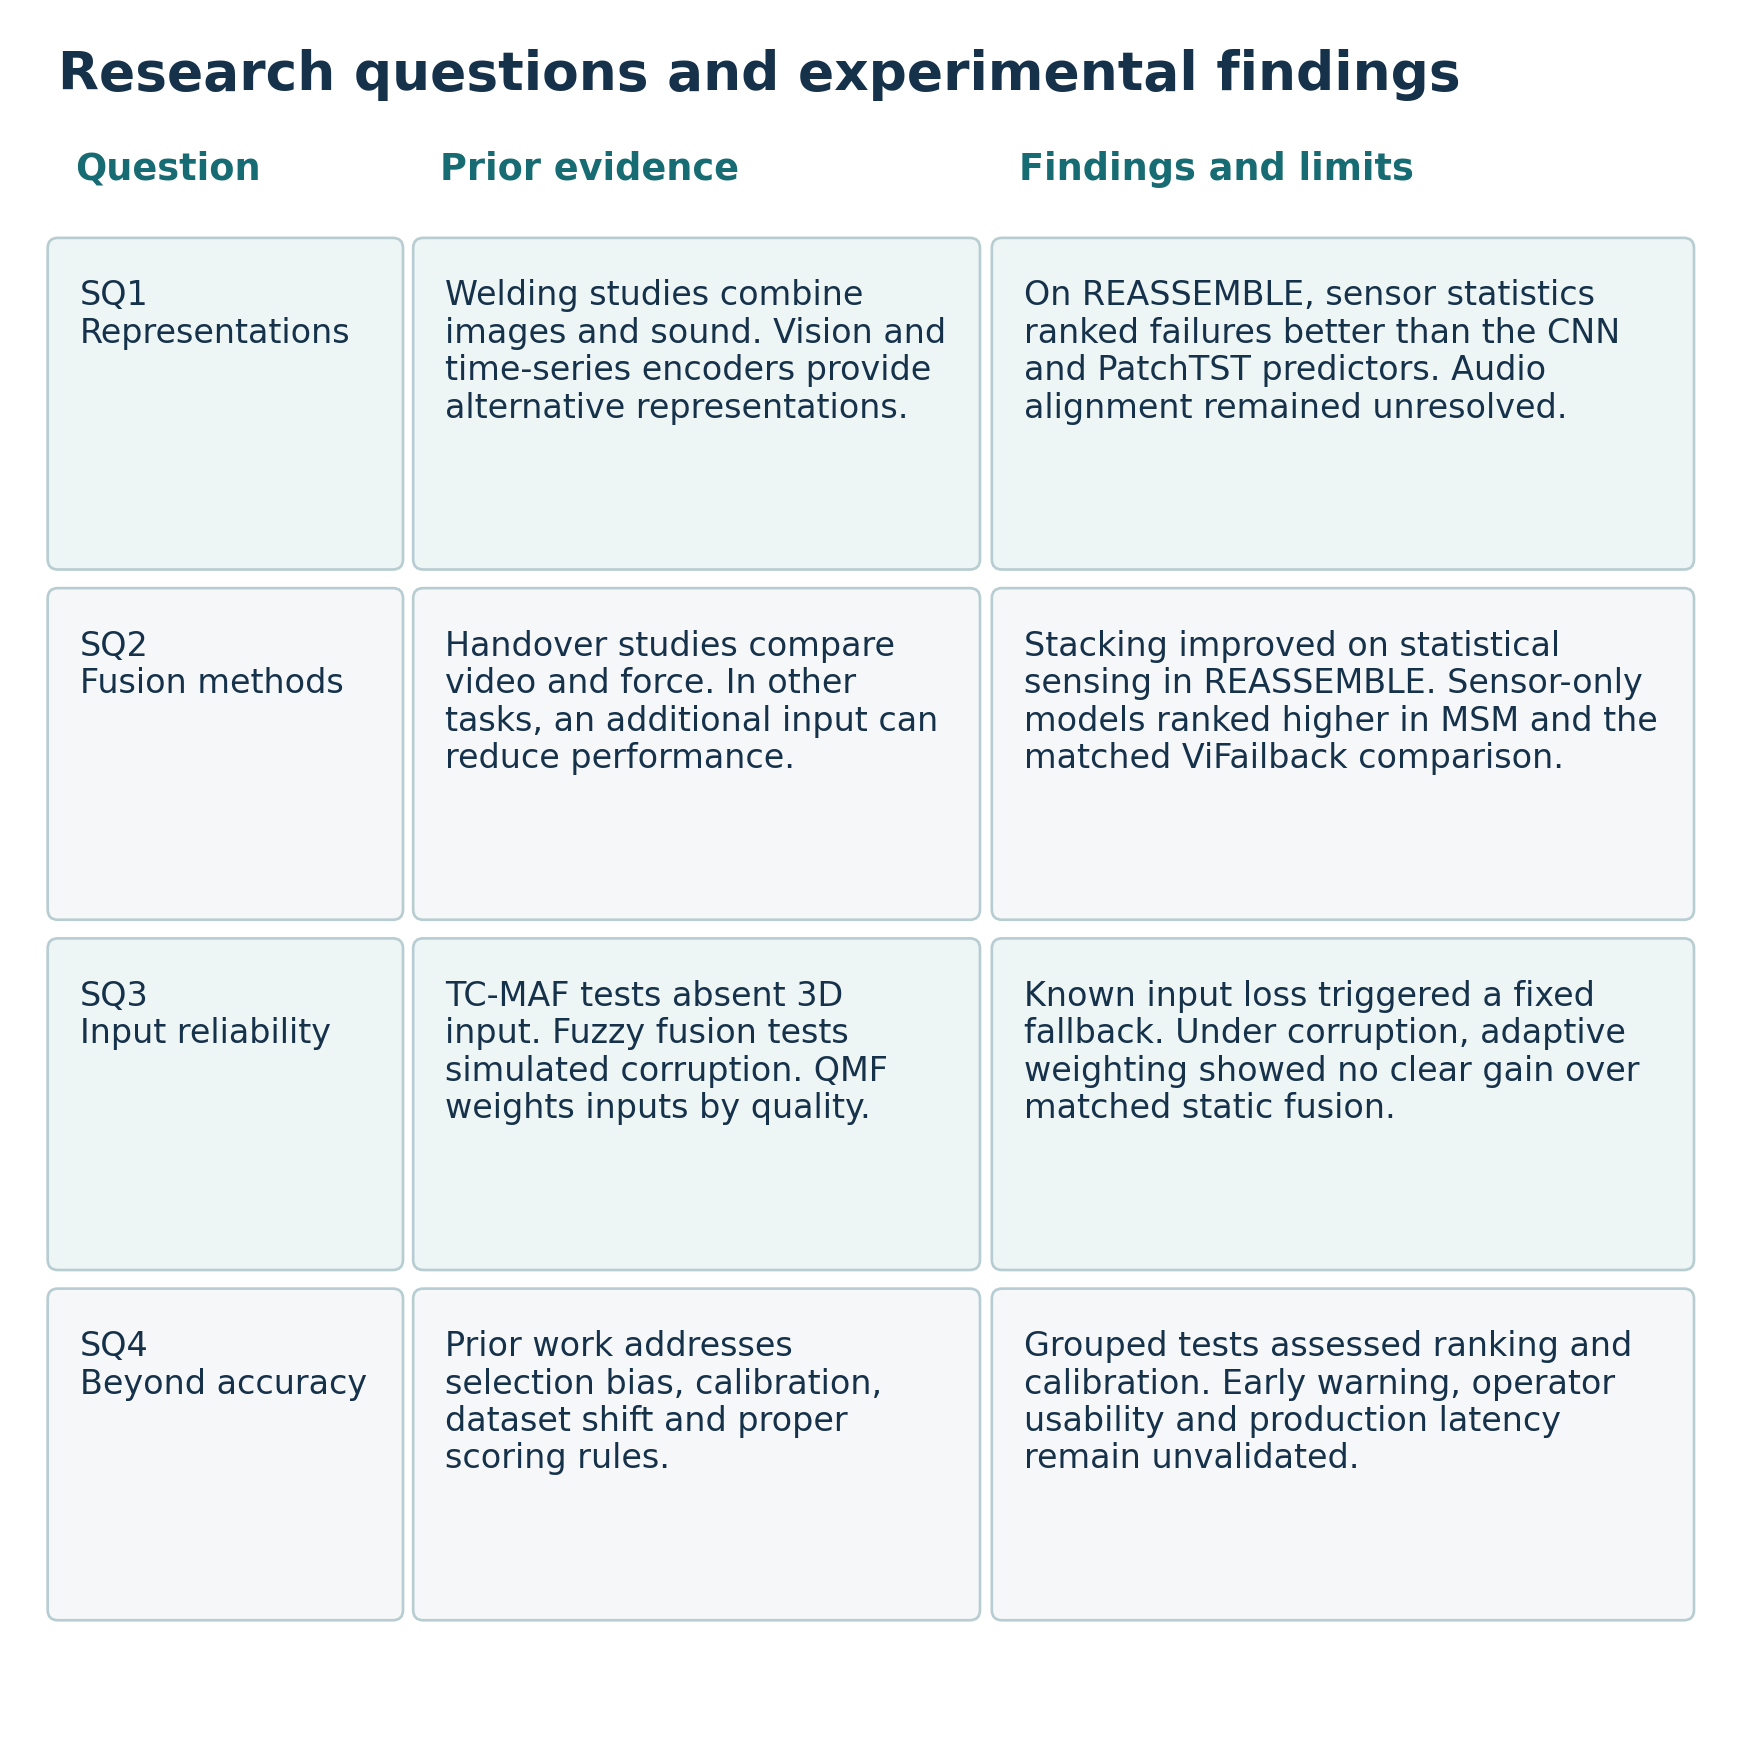
\includegraphics[width=\textwidth]{figures/gap_coverage.png}
\displaynote{The middle column summarises prior research. The right column gives the
corresponding experimental findings and limits.}
\end{figure}

\section{Threats to Validity and Unresolved Evidence}
Three features of the data limit a causal interpretation of architectural differences.
First, the target may only approximate the phenomenon of interest. PHM has no
independent quantitative tooth-damage reference, MSM's label mapping defines which
intervals count as abnormal, and some robotic outcomes remained ambiguous under visual
review. Second, the number of independently acquired units can be much smaller than the
number of predictions. Gear experiments, recording sessions, dates, tasks, and
participants capture different sources of dependence. Where identifiers were missing,
independence across those groups could not be verified. Third, several later analyses
revisited assessment populations examined during development. Intervals conditional on
fitted predictions and variation over a few seeds do not capture that selection history.

Preprocessing before the separate four-arm PHM loop limits attribution of its results to
architecture. In other experiments, differences in calibration, capacity, training
budget or corruption exposure accompanied architectural changes. Incomplete historical
PHM training-source lineage and unavailable ViFailback per-fit histories limit
independent reconstruction.\ev{Historical source and per-fit reconstruction limits}
{\EvidenceRef{E129}{}, \EvidenceRef{E130}{}, \EvidenceRef{E137}{}}
ViFailback's complete frozen/donor comparisons are supplemented by one-fold FULL20
evidence and separate hundred-epoch pilots; the adaptation contrasts remain
inconclusive. Whether the fine-tuning effect persists across the remaining task folds
and seeds is unknown, and corruption performance was unmeasured. The recorded forecast
was 43 additional GPU-days for the remaining FULL20 fits, with 47 days allowed including
variation and overhead. The central estimate scales the measured fitting rate by the
remaining split-specific workload. It is an estimated future runtime, not elapsed
GPU time or a confidence interval. This forecast covered
fine-tuning only (Section~\ref{sec:ch4-boundaries}).\ev{Completed adaptation scope and
recorded forecast}{\EvidenceRef{E113}{}, \EvidenceRef{E114}{}}
The literature synthesis covers the full texts available to a single reviewer.

Finally, the completed-window studies allowed the predictor to observe evidence near the
outcome. Synthetic blur, noise, or stream removal test specified interventions. They
give limited information about gradual calibration drift, unobserved timing faults, or
shifts to another physical machine. Transferring a predictor to an earlier decision time
or a different installation requires observations at that time and place.

\section{Implications for Multimodal System Design}
In a monitoring application, the intended decision determines what constitutes failure,
how it can be confirmed independently, and which observations arrive in time to be
useful. Evaluating each stream on the same held-out units establishes what it can
predict alone. Equal averaging and a fitted static combination then provide references
for testing whether context-dependent weights add value. When an instrument declares an
outage, the remaining predictor supplies a natural reference. When faulty values still
appear plausible, the relevant test is whether the gate recognises situations in which
trusting that stream would worsen the prediction.

A prospective return to welding could reserve whole welding sessions, collect an
independent weld-quality measure, and fix the prediction horizon before examining those
outcomes. On the same welds, exposure- and calibration-matched models could be assessed
for clean performance, known absence, degraded readings, timing error, and shifts
between operating conditions. Paired effects and a prespecified tolerance for
clean-performance loss would clarify the operational cost of any robustness gain. Such a
test would show whether the modest gain for completed assembly actions carries over to
weld-quality decisions.

\chapter{Conclusion and Future Work}
\label{ch:conclusion}

\section{Answer to the Main Research Question}
Combining camera and sensor predictions modestly improved completed-action failure
ranking over logistic sensing in REASSEMBLE. Logistic stacking achieved failure AP
0.4473, compared with 0.4294 for sensors and 0.4457 for equal probability averaging.
Equal averaging scored similarly, and its difference from stacking remained unresolved.
The result supports a conditional benefit from combining the available observations,
without establishing that a learned combiner was necessary.

The stacking gain over sensors did not recur in MSM or ViFailback. HANDOVER tested
averaging on an official split and also favored its sensor component, while unavailable
participant identities prevented the planned learned-fusion comparison. Across held-out
gear experiments, fusion of three sensor groups showed no clear improvement over the
training mean when predicting the photographic proxy, whose relationship to physical
tooth damage remained unvalidated.
Chapter~\ref{ch:discussion} gives the detailed contrasts and their study-specific
boundaries.

Together, the studies support evaluating each stream and simple fusion baselines before
adding adaptive weighting. Consistent adaptive benefit under degraded but present inputs
remained unresolved. The evidence concerns condition estimation and retrospective
assessment of completed events. It does not establish prospective weld-quality
decisions, which require an independently verified outcome and observations available
at a prespecified decision time.

\section{Supported Contributions}
\textbf{SQ1 --- Representation comparison.} The thesis compared statistical sensor
summaries, temporal encoders and visual representations under explicit task and fitting
conditions. It identified useful combinations of sensor representations and promising
visual pooling choices, while separating those findings from claims about learned
temporal order or universal encoder superiority.

\textbf{SQ2 --- Incremental fusion value.} The thesis estimated what fusion added over
single-input predictors and equal averaging on common assessment observations. The
contrasting assembly and external results show why a fusion claim depends on its
comparator, target and evaluation protocol.

\textbf{SQ3 --- Reliability under input failure.} The experiments distinguished
programmed fallback for a declared missing stream from adaptation to degraded inputs
that remained present. Matched-exposure comparisons tested whether learned weighting
added value beyond static fusion, leaving consistent adaptive benefit unresolved.

\textbf{SQ4 --- Interpretation beyond accuracy.} The evaluation combined ranking,
probability error, class-specific decisions, operating thresholds and grouped
uncertainty. This exposed cases in which better ranking did not imply better
probabilities or useful fixed-threshold decisions, and where changing the grouping
changed the uncertainty attached to the same predictions.

\section{Principal Limitations}
Each dataset imposes a different evidential limit. PHM lacks an independent
physical-damage reference, while native outcome definitions and ambiguous robotic events
constrain what the classification results mean. Incomplete identifiers for tools,
objects, sessions or participants limit claims of independence beyond the groups
actually checked.

Several follow-ups reused assessment populations examined during exploratory
development. Their intervals condition on saved fits and do not capture uncertainty from
the full selection process. Differences in calibration, training budgets and corruption
exposure also limit attribution of some contrasts to architecture. Preprocessing before
the separate four-arm PHM evaluation further compromises that diagnostic's isolation of
held-out observations.

Incomplete PHM historical training-source lineage and unavailable ViFailback per-fit
histories limit independent reconstruction beyond the retained configurations and
results. ViFailback target-CNN adaptation was assessed on one outer fold, with
inconclusive matched effects, so its consistency across task folds and seeds remains
unknown. Robustness to corrupted ViFailback inputs was not measured.

\section{Priorities for Future Research}
An independent welding study is the most direct next test of the original question. It
should establish weld quality through independent inspection, specify the prediction
horizon before examining outcomes, and reserve complete new welding sessions for
assessment. Camera and process measurements should cover only the information available
at that decision time. Warning time, false alarms and end-to-end delay would then
connect predictive performance to prospective use. For PHM, independent damage
measurements linked to known teeth would separate physical validity from agreement with
the photographic proxy.

For REASSEMBLE, a prespecified comparison on untouched recordings should test
last-quarter visual pooling, the same-sensor hybrid and anchored fusion separately and
in combination. Matched controls should preserve the relevant fitting, calibration and
corruption-exposure conditions to estimate their individual and joint effects. These
choices were promising in separate exploratory studies; their joint benefit has not
been established.

For ViFailback, extending matched fine-tuning across the remaining task folds and seeds
would test whether target-CNN adaptation changes visual ranking and fusion performance
consistently beyond the currently assessed fold. Missing, degraded and temporally
shifted inputs require a separate corruption study with its own scope and resource
estimate.

Secondary tests could examine HGB-based stacking in MSM and compare uncalibrated with
rank-preserving calibrated branch outputs in ViFailback, refitting F2 on each
corresponding training-side prediction bank. These are proposed comparisons with open
outcomes. Across them, fixed protocols, strong single-input controls and prespecified
tolerances for clean-performance loss would make any benefit easier to interpret.

\ifdefined\ThesisReviewCopy\else
\clearpage
% Use the top text margin for this standalone disclosure. The four paragraphs
% retain the manuscript's regular type size, margins and double spacing.
\begingroup
\makeatletter
\renewcommand{\@makeschapterhead}[1]{%
  {\parindent=0pt\raggedright\normalfont\Huge\bfseries #1\par}%
  \nobreak\vspace{6pt}}
\makeatother
\chapter*{AI Assistance Disclosure}
\addcontentsline{toc}{chapter}{AI Assistance Disclosure}
\endgroup
\noindent
The author defined the scope of the research, provided the implementation records and
saved experimental results, obtained full-text publications, and reviewed how the
methods and findings were interpreted and presented. Preparation of the manuscript
involved AI-assisted drafting and revision. The author used AI tools to develop and
refine the text, including the abstract, and to examine whether descriptions of the
models, experiments, and results were consistent with the available evidence.

The author conducted the literature research and critically reviewed the papers,
assessing how their methods, choice of baselines, and evaluation conditions supported
their findings. AI tools helped the author prioritise papers for closer reading, locate
relevant passages and tables during review, and organise the evidence into a comparison
matrix. AI tools also helped check bibliographic records and supported numerical
consistency checks, bibliography processing, APA citation editing, figure preparation
and LaTeX editing.
OpenAI Codex also helped prepare Figure~\ref{fig:review-depth} and
Table~\ref{tab:literature-synthesis}; the literature appraisals and their
interpretation are the author's.

The manuscript revision drew on existing publications, implementation records, and saved
experimental outputs, without new model training or inference on raw data. The thesis
distinguishes findings reported in publications, checks documented in earlier experiment
records, and checks performed on saved outputs during revision. Codex helped relate the
literature to the controlled experiments, recompute the core F2 ranking diagnostic and
reconcile the ViFailback completion records. AI-assisted appraisal formed part of the
same review process and provided no independent second human assessment. Ambiguous
source claims, incomplete experiments, and unresolved questions of physical validation
are documented as limitations.

Appendix~\ref{app:prompt-record} presents reconstructed paraphrases of implementation
and audit requests and describes AI assistance with evidence checks, revision and
archiving plans. These examples are not verbatim transcripts. OpenAI Codex
assisted with the implementation and audit tasks and with preparation of
Figure~\ref{fig:fusion-interfaces} \citep{OpenAICodex}. The records do not identify the
model version used in earlier implementation sessions.

\clearpage
\printbibliography[heading=bibintoc,title={References}]
\appendix
\chapter{Literature Search Records and Evidence Tables}
\label{app:literature}
\section{Literature Screening and Full-Text Appraisal}
Of 120 unique candidates, 39 met the inclusion criteria, 37 were excluded and 44
remained potentially relevant but insufficiently verified. For those 44 candidates,
the screening record identifies unverified modality identity or controlled evaluation
as the reason for leaving their status unresolved. Full-text appraisal covered 37 of
the 39 included works. The two accessible only through abstracts and bibliographic
metadata contributed to the screening counts but supplied no methodological or
numerical findings.\ev{Initial screening record and associated search logs dated 16 November 2026}{\EvidenceRef{E004}{},
\EvidenceRef{E007}{}, \EvidenceRef{E003}{}}

The subsequent appraisal covered 59 PDF files. Two pairs were byte-identical, leaving
\ExpandedPDFCount{} distinct files. Titles, authors, DOIs and repository identifiers
showed that these represented \ExpandedPDFCount{} additional works, bringing the total
appraised to \ReviewWorkCount{}. This historical total includes empirical industrial
studies, transferable methods, statistical and representation methods, dataset
descriptions and contextual studies. \citet{Ting1999Issues} informed the stacking methodology and is cited separately from
the \ReviewWorkCount{} works included in the full-text appraisal.

The search log for this screening round records more than 15 distinct queries. Several
queries returned results together, precluding an exact count of the records retrieved by
each. The subsequent appraisal drew on additional accessible full texts and used
publisher or repository pages to check bibliographic identities and versions. This
procedure limits the review's coverage to the works identified and accessible through
these routes.\ev{Expanded appraisal and counts}{\EvidenceRef{E014}{},
\EvidenceRef{E008}{}, \EvidenceRef{E009}{}, \EvidenceRef{E010}{}}

\section{Extraction, Locators, and Versions}
For each study, the appraisal recorded the prediction unit and target, physical inputs,
derived representations, fusion method, single-input comparisons and assignment of data
to training and evaluation. Missing inputs, noisy inputs and changes of operating
conditions were coded separately. Numerical findings cite the relevant page, table or
figure. Where the available text left a procedure unspecified, its status was recorded
as unknown.

The appraisal distinguishes the published bibliographic record from the version
examined. Preprints and journal articles sometimes give different sample counts for the
same work. File hashes identify the version used for each extraction. The 37 initial
full-text records include 148 short quotations that locate the evidence for their codes.
The review compared reported methods and results without rerunning the published
experiments.\ev{Extraction and identity records}{\EvidenceRef{E005}{},
\EvidenceRef{E006}{}, \EvidenceRef{E015}{}, \EvidenceRef{E012}{}}

\section{Comparison Matrix and Denominators}
Table~\ref{tab:literature-matrix} gives the codes for the initial 37 studies.
Table~\ref{tab:expanded-register} identifies the contribution and principal limitation
of each of the 57 additional works. The accompanying matrix gives the missing-input,
noise and shift tests for individual studies, together with source locations.\ev{Full
expanded comparison register}{\EvidenceRef{E011}{}, \EvidenceRef{E013}{}}

Within-protocol input variants do not guarantee equal capacity, pretraining, calibration
or selection budget. Planned single-input deployment, missing training images, generated
substitution, stochastic dropout and unexpected inference outage are different
conditions. Ordinary defective objects, natural geometric gaps and fixed noisy data are
not automatically controlled corruption experiments. The codes describe this inspected
evidence and cannot estimate field-wide prevalence.

\begin{longtable}{@{}p{0.33\textwidth}llllll@{}}
\caption{Comparison of the 37 Original Full-Text Studies}\label{tab:literature-matrix}\\
\toprule Study & Data & Fusion & Base & Missing & Noise & Shift \\
\midrule\endfirsthead
\toprule Study & Data & Fusion & Base & Missing & Noise & Shift \\
\midrule\endhead
\parencite{Wang2025A} & VIB & H & U & N & S & A \\
\parencite{Ying2025Trustworthy} & CAM-S & H & M & N & S & N \\
\parencite{Huang2026Rolling} & AUD-VIB & I & M & N & S & C \\
\parencite{Gu2024Improved} & AUD-VIB & I & P & N & N & N \\
\parencite{Yang2024Fault} & MS & I & M & PA & N & N \\
\parencite{Ma2025A} & IMG-U & I & M & TR & N & N \\
\parencite{Li2025PGMTKD} & MS & KD & R & PA & N & N \\
\parencite{AlDulaimi2019A} & SV & I & L & N & S & N \\
\parencite{Li2025MADFlow} & RGB-G & I & A & N & N & N \\
\parencite{Wan2024Pipeline} & AUD & E & M & N & N & N \\
\parencite{Baltrusaitis2019Multimodal} & X & TAX & S & NA & NA & NA \\
\parencite{Sui2026Incomplete} & RGB-G & KD+L & M & PA & N & N \\
\parencite{Cheng2025Multimodal} & RGB-G & H & M & N & N & N \\
\parencite{Xu2025ModalityResilient} & RGB-G & KD+H & P & SD & N & N \\
\parencite{Shangguan2025CPIR} & RGB-G & H & A & N & N & N \\
\parencite{Altinses2025Performance} & SIM-CS & I & A & GS & N & T \\
\parencite{Wang2023Multimodal} & RGB-G & H & M & N & N & N \\
\parencite{Horwitz2023Back} & RGB-G & E & M & N & N & N \\
\parencite{Costanzino2024Multimodal} & RGB-G & H & A & N & N & N \\
\parencite{Rudolph2023Asymmetric} & RGB-G & I & M & N & N & N \\
\parencite{Bonfiglioli2023The} & SIM-G & E & M & N & N & N \\
\parencite{Bergmann2022The} & RGB-G & E & P & N & N & N \\
\parencite{Wang2020What} & X & I & M & N & N & N \\
\parencite{Xie2025Audiovisual} & CAM-S & I+KD & M & PA & S & N \\
\parencite{Goodarzi2023Deep} & MS & E+I & M & N & S & N \\
\parencite{Roth2022Towards} & RGB & U & U & N & N & N \\
\parencite{Bergmann2019MVTec} & RGB & U & U & N & N & N \\
\parencite{Purohit2019MIMII} & AUD & U & U & N & B & N \\
\parencite{Koizumi2019ToyADMOS} & AUD & U & U & N & B & N \\
\parencite{Koizumi2020Description} & AUD & U & U & N & F & N \\
\parencite{Chu2024A} & AUD-VIB & I & N & N & N & A \\
\parencite{Kullu2022A} & MS & I & M & N & N & N \\
\parencite{Chen2023Multisensor} & CAM-S & E & M & N & N & N \\
\parencite{Li2022A} & OPT-AUD & I & M & N & N & N \\
\parencite{Petrich2021Multimodal} & CAM-S & I & M & RS & N & N \\
\parencite{Pandiyan2022Deep} & OPT-AUD & E & N & N & N & W \\
\parencite{Bevans2023Heterogeneous} & MULTI-CAM & E & A & N & N & B \\
\bottomrule
\end{longtable}
\displaynote{All 37 records have evidence status F. The codes describe the inspected
protocol. They do not rate study quality.}
\noindent\textit{Data:} CAM-S denotes a physical camera and a separate non-image signal;
RGB-G denotes RGB and geometry; OPT-AUD denotes photodiode and acoustic signals, without
a camera input. MS denotes machine/process channels; SV denotes parallel representations
of the same telemetry; IMG-U has incompletely documented image provenance. SIM-CS/SIM-G
are synthetic. RGB, AUD and VIB are single physical modalities; MULTI-CAM uses several
imaging sources; X is transferable non-industrial evidence.
\par\noindent\textit{Fusion:} E, early; I, intermediate; L, output-score fusion; H,
hybrid feature/output fusion; KD, privileged cross-modal training; U, unimodal; TAX,
taxonomy. Authors' terminology is normalised by where information is combined.
\par\noindent\textit{Baseline:} M, input variants evaluated within one protocol; P,
partial/ambiguous; R, retained-input student with/without teachers; L, literature
comparison; A, module/map/task ablations only; U, unimodal reference; S, survey; N, not
established. M does not guarantee matched capacity, pretraining or tuning.
\par\noindent\textit{Missing:} PA, planned missing-input inference; SD, simulated
dropout; TR, missing training images with complete tests; GS, generated substitution;
RS, retrained input subsets; N, no controlled trial established; NA, survey.
\textit{Noise:} S, synthetic intervention; B, recorded-background mixing; F, fixed noisy
benchmark; N, no controlled trial established. \textit{Shift:} A, target-adaptive
transfer; C, condition transfer with target validation; B, independent-build/layout
transfer with limited outcome coverage; T, simulated translation; W, unseen window
duration; N, no held-out domain transfer established.


\begingroup\small
\begin{longtable}{@{}P{.25\textwidth}P{.16\textwidth}P{.53\textwidth}@{}}
\caption{Full-Text Appraisal of the 57 Additional Works}\label{tab:expanded-register}\\
\toprule Work & Evidence role & Appraisal focus and qualification \\
\midrule\endfirsthead
\toprule Work & Evidence role & Appraisal focus and qualification \\
\midrule\endhead
P001 \parencite{P001} & Context & Single infrared image restoration; no independently
acquired second modality. This is context rather than evidence for a fusion advantage.
\\
P002 \parencite{P002} & Context & Infrared machinery diagnosis. Combining thermal regions
remains image-only; vibration fusion is proposed as future work. \\
P003 \parencite{P003} & Industrial & Physical camera and audio welding classification. Split
independence and controlled missing/noise evaluation are not established in the
inspected postprint. \\
P004 \parencite{P004} & Methods & Seminal evaluation foundation on model-selection bias. It
does not supply an industrial fusion experiment. \\
P005 \parencite{P005} & Methods & Transferable modality-dropout method. Training exposure
and planned available-input configurations determine the robustness claim. \\
P006 \parencite{P006} & Methods & Transferable gated intermediate fusion. Learned allocation
alone does not establish calibrated modality reliability. \\
P007 \parencite{P007} & Methods & Transferable robust multimodal classification
architecture. The inspected preprint and published journal metadata refer to one work.
\\
P008 \parencite{P008} & Methods & Predictive uncertainty under dataset shift. Good
in-distribution confidence does not guarantee shifted reliability. \\
P009 \parencite{P009} & Methods & Reproducibility and reporting foundation. Documentation
and code availability are distinct from independently reproduced results. \\
P010 \parencite{P010} & Methods & The visual patch Transformer was evaluated on image
recognition. The study provides no comparison of the industrial visual models evaluated
here. \\
P011 \parencite{P011} & Methods & The audio-spectrogram Transformer represents sound through
spectrogram patches. The present studies include no completed audio-branch comparison.
\\
P012 \parencite{P012} & Methods & Self-supervised dilated-convolution time-series encoder.
It is not a Transformer; the reported Transformer substitution performs worse. \\
P013 \parencite{P013} & Methods & The video Transformer models interactions across space and
time. The REASSEMBLE visual classifier averages frame descriptors over time. \\
P014 \parencite{Nagrani2021MBT} & Methods & Audiovisual attention-bottleneck fusion.
Transferable representation design does not establish industrial sensor-failure
robustness. \\
P015 \parencite{P015} & Methods & Multimodal benchmark and evaluation framework. Its
different tasks are not independent replications of one industrial target. \\
P016 \parencite{P016} & Methods & The missing-modality Transformer evaluation includes
adverse multimodal results. For the Food dataset, the prose and tabulated unimodal
result disagree. \\
P017 \parencite{P017} & Methods & The preprint and published article on leakage in
scientific evaluation give different counts of affected papers. \\
P018 \parencite{P018} & Methods & The study evaluates pretrained time-series representations
on benchmarks. Transfer of its weights to the industrial tasks considered here was not
tested. \\
P019 \parencite{Sliwowski2025REASSEMBLE} & Dataset & The robotic assembly dataset provides
native action outcomes. Its published demonstration count differs from the eligible
sample for the present action-level analysis. \\
P020 \parencite{P020} & Methods & Transferable multimodal negative-learning study. Its noise
regimes and negative comparisons remain specific to the reported tasks. \\
P021 \parencite{P021} & Industrial & Physical tool images and force measurements with
adaptive fusion. Post-pass image timing and incompletely reported splits limit
prognostic claims. \\
P022 \parencite{P022} & Methods & Non-industrial dynamic-fusion method. Its evidence informs
fusion assumptions without constituting industrial deployment validation. \\
P023 \parencite{P023} & Methods & Transferable constrained fusion of text with time series.
It supplies negative evidence against assuming every additional modality helps. \\
P024 \parencite{P024} & Industrial & Industrial inspection using geometric prior
information. RGB and geometry are distinguished from independent machine telemetry. \\
P025 \parencite{P025} & Industrial & The industrial inspection model combines visual and
geometric features with language for defect reporting. Its evaluation includes
task-specific supervision and measures report consistency. \\
P026 \parencite{P026} & Industrial & Train-calibrated RGB/geometry fusion includes explicit
missing-3D evaluation and static/gated controls. It is not camera-plus-machine-telemetry
evidence. \\
P027 \parencite{P027} & Industrial & Audio, vibration and current fusion with missing-input
claims. Limited auditability excludes it from strong quantitative synthesis. \\
P028 \parencite{Thoduka2024Handover} & Dataset & Completed robotic handover outcomes with
video, force/torque and gripper inputs. Added gripper input reduces one five-class
accuracy result. \\
P029 \parencite{Huo2022Multisensor} & Industrial & Thermal-image and vibration fault
diagnosis with single-input and noise controls. Reliability conclusions remain
conditional on its protocol. \\
P030 \parencite{Nie2023PatchTST} & Methods & PatchTST was evaluated for time-series
forecasting. The PHM regression and REASSEMBLE classification experiments trained
separate temporal models from scratch. \\
P031 \parencite{P031} & Industrial & Vision-language surface localisation is evaluated with
pixel metrics. These measure localisation rather than image-level detection or numerical
process sensing. \\
P032 \parencite{Hua2026Weld} & Industrial & Camera/audio weld-penetration attention fusion.
Clean single-input and fused models all report 100\% accuracy; independent-run splitting
is unclear. \\
P033 \parencite{P033} & Industrial & RGB/geometry disagreement scoring. Eyecandies image
AUROC decreases despite improved localisation, showing metric-specific trade-offs. \\
P034 \parencite{P034} & Methods & Space-time attention models cross-frame interactions. The
core REASSEMBLE visual representation averages frame descriptors. \\
P035 \parencite{P035} & Context & Weakly supervised single-camera surface inspection.
Internal feature fusion is not fusion of independently acquired physical modalities. \\
P036 \parencite{P036} & Methods & Transferable counterargument on attention interpretation.
Model inspection does not by itself establish a physical causal explanation. \\
P037 \parencite{Altinses2023Fuzzy} & Simulation & Camera/robot telemetry corruption in
simulated pose regression. Overlapping temporal windows and random splitting limit
physical-deployment inference. \\
P038 \parencite{P038} & Industrial & RGB/geometry consistency fusion. Its learned scalar
mixing coefficient does not demonstrate sample-conditioned online reliability
adaptation. \\
P040 \parencite{Bengio2004CVVariance} & Methods & Cross-validation variance theory.
Overlapping training folds do not supply independent replications for a naive standard
error. \\
P041 \parencite{Guo2017Calibration} & Methods & Validation-fitted calibration foundation.
In-distribution temperature scaling is not a guarantee of reliable probabilities after
shift. \\
P042 \parencite{P042} & Context & Single-vibration diagnosis with synthetic noise. Simulated
target training and reporting inconsistencies limit transfer and field-validity claims.
\\
P043 \parencite{P043} & Methods & Distribution-shift benchmark. OOD validation access is
explicit; this is not an untouched-target industrial multimodal experiment. \\
P044 \parencite{P044} & Methods & Transferable medical fusion counterexample. Selection and
evaluation share validation data; no independent final test is established. \\
P045 \parencite{P045} & Industrial & Post-pass tool photographs and acoustic emission
predict wear. Strong visual and adverse multimodal comparators coexist with unresolved
tool-split coverage. \\
P046 \parencite{P046} & Industrial & Microphone/accelerometer bearing fusion. Test-noise
results lack an equivalent static corruption comparator; recording-disjoint splitting is
unclear. \\
P048 \parencite{P048} & Industrial & Thermal-camera and vibration feature fusion.
Overlapping windows, multirate pairing and separately fitted speeds restrict
generalisation claims. \\
P049 \parencite{P049} & Methods & Transferable attention-interpretability critique.
Attention perturbation is distinct from physical input corruption or modality dropout.
\\
P050 \parencite{P050} & Methods & Transferable unaligned language/audio/video
cross-attention. Unequal feature rates are not a controlled hardware-clock offset test.
\\
P051 \parencite{P051} & Industrial & Visible/infrared federated detection. Incomplete
clients differ from surprise inference outage; group splits, clipped results and
coefficient conflicts limit appraisal. \\
P052 \parencite{Kim2026MSM} & Dataset & Milling dataset with laboratory video and machine
measurements. Dataset availability enables research but is not itself a learned fusion
result. \\
P053 \parencite{P053} & Industrial & Audio/vibration wavelet-image cross-attention. These
are transformed signals, not camera images; controlled missing/noise tests are not
established. \\
P054 \parencite{P054} & Industrial & RGB/surface-normal anomaly detection. Training
feature-noise regularisation is distinct from a test-input degradation benchmark. \\
P055 \parencite{P055} & Methods & Proper-scoring-rule foundation. Expected propriety does
not certify finite-sample calibration or shifted sensor reliability. \\
P056 \parencite{P056} & Industrial & RGB/point-cloud local alignment preprint, version 1.
Checkpoint-selection population and retraining variability remain unclear. \\
P057 \parencite{Zeng2026ViFailback} & Dataset & The study uses visual symbols and language
to diagnose manipulation failures. The present ViFailback experiment instead combines
camera views and numerical robot observations. \\
P058 \parencite{Zhang2023QMF} & Methods & Transferable quality-aware weighting. Its
conditional generalisation-upper-bound comparison does not imply universal actual-risk
superiority. \\
P059 \parencite{Zhao2024RTDETR} & Methods & Single-image object detector foundation.
Executing an extracted CNN backbone does not execute the full detector or its reported
inference pipeline. \\
\bottomrule\end{longtable}
\displaynote{The accompanying CSV identifies each target, fusion method, control, test
of missing, noisy, or shifted inputs, result, and source location. The role column
distinguishes direct experimental evidence from background material.}\endgroup
\noindent\textit{Interpretation:} Transferable methods are non-industrial unless their
record identifies a direct application. Dataset papers and unimodal/context references
do not supply a multimodal fusion experiment. A retained preprint remains provisional.
All source versions, complete qualifications and numerical locators are in the expanded
register.


\section{Benchmark Identity and Assessment Populations}
The MVTec 3D-AD dataset paper lists 249 anomaly-free and 948 anomalous test samples, a
total of 1,197. It reports 2,656 training and 294 validation samples separately
\citep[Table~1, PDF p.~4]{Bergmann2022The}. UCF reports the same test count
\citep{Cheng2025Multimodal}, whereas some other method descriptions give 1,137. The
discrepancy leaves the samples underlying those comparisons uncertain. The review uses
the published scores, whose comparability also depends on preprocessing, masks and
metric definitions.

\chapter{Dataset Inventories, Exclusions, and Target Definitions}
\label{app:datasets}

\section{Registry Conventions}

Table~\ref{tab:dataset-registry} distinguishes the number of observations in each
published release from the number eligible for a particular experiment. Eligibility
depended on the target, the required inputs and the temporal correspondence between
them. The counts refer to the dataset versions used in the reported experiments.

\begingroup\small
\begin{longtable}{@{}P{.17\textwidth}P{.25\textwidth}P{.25\textwidth}P{.23\textwidth}@{}}
\caption{Prediction Targets, Units, and Eligible Populations}\label{tab:dataset-registry}\\
\toprule Dataset & Target and unit & Admitted population & Qualification \\
\midrule\endfirsthead
\toprule Dataset & Target and unit & Admitted population & Qualification \\
\midrule\endhead
PHM & Provisional image-derived candidate-area regression; tooth/run values and
aggregated run target & v3: 20 run records, 24 teeth per run, 480 tooth/run values
across EXP-A/B/F & Image reference is privileged/offline; only three experiment groups
support the retained LOEO setting \\
REASSEMBLE & Completed high-level action failure; failure positive & 4,530 actions, 509
failures, 148 recordings & Hand camera plus five sensor streams; 149 recordings in raw
inventory \\
MSM & Native label 1 versus labels 0/2; cutting interval & 1,895 intervals: 336 positive,
1,559 negative & 2,512 native intervals; 617 technical exclusions; 45 nominal experiment
groups \\
ViFailback & Native whole-episode outcome, with failure positive & 4,382 episodes across
99 tasks (3,753 failures and 629 successes) & 5,202 native episodes, with 820 excluded
or quarantined after reconciliation \\
HANDOVER & Handover failure; failure positive & 587 eligible trials: 335 train, 101
validation, 151 test & 589 native trials; two training exclusions; test 110 failure/41
success \\
Intel welding & Original industrial-monitoring setting & No independent weld-quality
fusion evaluation & Feasibility-gate exclusion; not a trained-model performance result
\\
\bottomrule
\end{longtable}
\endgroup


\section{Target Lineage and Pairing}

The PHM target \nolinkurl{phm2026_image_damage_v3} uses one deterministic view per
tooth (teeth 5--28) and averages the three highest tooth values per run. It remains a
provisional photographic proxy for physical deterioration. Earlier targets differ in
image geometry, view aggregation and tooth sets, limiting error comparisons. Sorted
profiles retain the within-run distribution but discard tooth identity. The fixed
image split and sensor leave-one-experiment-out protocol assess different populations.\ev{PHM target
lineage and model mapping}{\EvidenceRef{E021}{}, \EvidenceRef{E108}{}}

The REASSEMBLE release reports 4,551 demonstrations; 4,530 completed pick, insert,
remove and place actions met the primary-action and input-completeness criteria,
including 509 failures. Each action supplied 22 scalar sensor channels and a descriptor
from 16 hand-camera frames. Audio was excluded because correspondence between
annotation and waveform times could not be independently established.\ev{REASSEMBLE cohort and
gates}{\EvidenceRef{E042}{}, \EvidenceRef{E039}{}}

\section{External Cohorts and Exclusions}

MSM predicts intervention-worthy abnormal behaviour (native label 1) against labels 0
and 2. Label 2 denotes stable cutting with a defective tool, distinct from label 1.
Excluding its 125 intervals leaves 1,770 observations. The 45 nominal experiment
groups, seven machine/date proxies and five calendar dates are not interchangeable;
the date-level evidence has few independent clusters. Technical exclusions establish
usability, not that excluded intervals were uninformative.\ev{MSM admitted cohort and target semantics}{\EvidenceRef{E073}{},
\EvidenceRef{E072}{}, \EvidenceRef{E067}{}}

ViFailback contains 5,202 native episodes, with 4,545 failures and 657 successes. Two
camera-quality exclusions reduced a provisional cohort of 4,384 episodes to 4,382. The
820 excluded or quarantined episodes count each episode once even when several exclusion
reasons apply. The historical and later matched CNN conditions assess the same 4,382
episodes under different fitting procedures. Repeated seeds and outer folds reuse these
episodes.\ev{External dataset reconciliation and current result
boundaries}{\EvidenceRef{E106}{}, \EvidenceRef{E107}{}}

HANDOVER retained 587 of 589 trials under the native partitions and paired-input
requirement. Two training trials exceeded the 0.1~s nearest-wrench alignment limit.
All 151 test trials (110 failures, 41 successes) remained. Higher failure prevalence
than REASSEMBLE affects failure-class AP comparisons. Participant-level independence
could not be verified.

\chapter{Model Configurations and Implementation Details}
\label{app:implementation}

\section{Executed Component Boundaries}
The PHM scalar-image regressor and the REASSEMBLE action classifier use different
components of RT-DETR. Table~\ref{tab:component-boundaries} identifies the model
weights, intermediate representation and output used by each branch.

\begin{table}[htbp]
\caption{Inputs and Outputs of the Executed Model Components}\label{tab:component-boundaries}
\centering\small

\begin{tabular}{P{0.19\linewidth}P{0.34\linewidth}P{0.37\linewidth}}\toprule
Component & Input and representation & Executed boundary\\\midrule
PHM scalar image branch & Three spatially pooled 256-dimensional maps, plus recorded
extraction latency: 769 actual head covariates & Ultralytics RT-DETR-L prediction path
with hooked maps; not the CNN-only REASSEMBLE path\\
REASSEMBLE visual branch & Sixteen RGB frames pooled to an 896-dimensional action
descriptor & Frozen ResNet18-vd CNN backbone inside RT-DETR-R18vd, followed by a trained
binary head\\
REASSEMBLE numerical statistics & 22 channels, ten statistics each: 220 features &
Training-only standardisation and logistic regression\\
REASSEMBLE temporal branch & 512 progress positions by 22 channels & Scratch-initialised
compact PatchTST and fitted projection/head\\
External numerical adapters & MSM: 90; HANDOVER: 36; ViFailback: 280 statistics &
Dataset-specific input construction; not an unchanged raw-sequence temporal
encoder\\\bottomrule
\end{tabular}
\displaynote{The reported dimensions apply to the listed implementation paths.}
\end{table}
\ev{Executed component map}{\EvidenceRef{E108}{}}

The REASSEMBLE extractor accesses the CNN through
\nolinkurl{wrapper.model.backbone.model}; the detector encoder, decoder and box heads
are bypassed.

The PHM scalar-image head receives extraction latency alongside pooled image features.
The dependence of latency on the computing environment limits attribution of the
regressor's performance to image content. The target measures candidate area in
photographs. Earlier target versions selected the maximum across views, while the
retained version uses a fixed view for each tooth. The top-three run summary aggregates
the tooth values. Independent physical defect masks were unavailable to validate
localisation.

\subsection{Shared RGB Preprocessing}
\label{sec:rtdetr-preprocessing}
For the \texttt{PekingU/rtdetr\_r18vd} checkpoint at revision
\nolinkurl{ac77a11ff0170a41b771c03264987f8ce2b0d753}, the retained processor uses
bilinear resizing to $640\times640$ and RGB rescaling by $1/255$.
ImageNet mean/standard-deviation normalisation is disabled
(\texttt{do\_normalize=false}), even though the configuration lists mean and standard-deviation
values. This preprocessing applies to the specified REASSEMBLE and ViFailback
paths; the PHM Ultralytics detector uses its separate implementation.\ev{Pinned processor
and checkpoint identity}{\EvidenceRef{E146}{}, \EvidenceRef{E149}{}}\ev{ViFailback
processor reuse}{\EvidenceRef{E092}{}, \EvidenceRef{E095}{}}

\section{Temporal Representations}
The PHM implementation defines a compact channel-independent PatchTST-style regressor
with default patch length sixteen, stride eight, hidden width 32, four attention heads,
two encoder layers, feed-forward width 64, dropout 0.1 and a 64-unit head. The
configured input width remains run-specific. A scalar output and the optional
sorted-profile head answer different target questions. The latter uses a base and
positive softplus increments to enforce ascending order; this guarantees an
order-statistic profile but discards tooth identity. The monotonicity does not
demonstrate that the estimated profile matches actual damage.\ev{PHM temporal
configuration}{\EvidenceRef{E029}{}}

The REASSEMBLE temporal branch follows a separate configuration: patch length 32, stride
sixteen, width 32, two layers, four heads, feed-forward width 64 and dropout 0.1. It
begins without pretrained temporal weights. Mean patch pooling and channel concatenation
feed a 128-dimensional projection and binary head, yielding 109,505 parameters in the
configured implementation. With internal scaling and input masking disabled, the observed-value mask does not
suppress missing tokens in attention. The encoder processes 31 patches per channel;
residual missing values are filled using training-only normalisation before encoding.
These are properties of the configured implementation, not guarantees implied by the
model family \parencite{Nie2023PatchTST}.\ev{REASSEMBLE temporal
recipe}{\EvidenceRef{E051}{}}

\section{Heads, Fitting and Calibration}
The original visual head is a new 896--128--1 network with ReLU and dropout 0.1,
containing 114,945 trainable parameters above a frozen backbone. Original visual epoch
candidates are five and ten; temporal candidates are three and six. Both use AdamW with
learning rate 0.001, weight decay 0.001 and batch size 128. These candidates constitute
the recorded selection procedure, not a broad optimiser search. Logistic regression
separately compares $C\in\{0.1,1,10\}$ under inner-fold selection.\ev{Original branch
configuration}{\EvidenceRef{E051}{}}

Branch calibration used an unweighted sigmoid logistic fit to the selected inner
out-of-fold scores. The outer assessment labels were withheld from calibration. The
original procedure selected a threshold between 0.01 and 0.99 by maximising inner
out-of-fold balanced accuracy, resolving ties toward 0.5. Later studies used a fixed
threshold of 0.5. Comparisons between those procedures therefore combine the effects of
model and threshold changes.

\section{Fusion Mechanisms and Attribution}
In the original REASSEMBLE procedure, uniform fusion averages the two calibrated branch
probabilities. F2 fits an unweighted L2 logistic model to those probabilities, with
$C=1$ and a new intercept and two coefficients. It is neither an F-beta metric nor a
convex weighted average. Its
coefficients depend on score scaling and are not causal percentages of modality
importance.

Feature fusion F3 combines a 128-dimensional visual projection with the 220 statistical
numerical features through separate projections, normalisation and a fitted classifier.
Its recorded candidates use hidden widths 32 or 64 and ten or twenty epochs. Context
gates instead allocate weights over branch logits. Their candidates have hidden width
eight or sixteen and forty epochs. Action-only, quality-only and combined contexts
remain different models, as do a static gate with context held constant and a gate
exposed to corrupted OOF records.\ev{Fusion and gate
configurations}{\EvidenceRef{E052}{}}

With one branch available, the explicitly masked convex-logit gate gives that branch a
weight of one. The resulting prediction follows from the specified masking rule. When
both branches are absent, some implementations reject the input and the external
evaluation records abstention and coverage.

The later anchored adjustment is another distinct mechanism. It modifies frozen F2
probability coefficients by bounded context-dependent factors, with a zero-initialised
adaptive output. It is not the same convex logit gate and need not have the same
calibration or threshold policy. Appropriate static and exposure-matched controls are
necessary to identify what, if anything, adaptation adds.\ev{Anchored
implementation}{\EvidenceRef{E061}{}}

\section{External Adaptations}
MSM and HANDOVER use the shared frozen visual backbone with a newly trained head and a
dataset-specific numerical classifier.\ev{External model register}{\EvidenceRef{E106}{}}

MSM fixes the HGB sensor control at 100 iterations, learning rate 0.1, fifteen maximum
leaf nodes, minimum leaf size ten and L2 regularisation 1.0, with early stopping
disabled. Training-only inverse-class-frequency sample weights balance its loss; these
settings were not selected by a hyperparameter search. The logistic sensor branch uses
training-only standardisation, balanced L2 logistic regression with $C=1$, the L-BFGS
solver and at most 2,000 iterations. Original F2 uses the same solver, iteration limit
and $C$, but is unweighted and fits a new intercept and two coefficients to clean
group-OOF branch probabilities. The primary evaluation fits no separate calibrator and
uses a fixed threshold of 0.5.\ev{Fixed MSM model and fusion configuration}{\EvidenceRef{E066}{},
\EvidenceRef{E147}{}, \EvidenceRef{E148}{}}

ViFailback adds pooling across three camera views. Its matched study compares frozen
generic and transferred CNN weights with a fresh target head in each case. Scalers,
sigmoid calibrators and out-of-fold fusion coefficients were fitted to target data
where specified. FROZEN20 and DONOR20 provide complete three-seed, three-outer-fold
assessments. FULL20 covers seed~42, outer fold~0 and its three inner fits; FULL100 is a
single-role pilot alongside FROZEN100 and DONOR100. Missing, degraded and temporally
shifted input conditions remain unmeasured. Table~\ref{tab:vif-status} gives the exact
fit counts and assessment scope.\ev{Completed ViFailback comparison scope}{\EvidenceRef{E113}{},
\EvidenceRef{E114}{}}

\chapter{Supplementary Results and Sensitivity Analyses}
\label{app:supplementary-results}

\section{Matched Two-Epoch Representation Diagnosis}
The preceding four-arm study compared sixteen and thirty-two frames under unequal epoch
budgets. Table~\ref{tab:fourarm-visual-supplement} retains its results separately from
the later matched diagnostic. All four arms used the same 4,530 actions, five outer
folds and seed family~42.

\begin{table}[htbp]
\caption{Earlier Four-Arm Visual Comparison on the Common REASSEMBLE Cohort}
\label{tab:fourarm-visual-supplement}
\centering\small
\begin{tabular}{lrrrrr}\toprule
CNN state & Frames & Epochs & Visual AP & Sensor AP & F2 AP\\\midrule
Frozen & 16 & 5 & 0.221644 & 0.420803 & 0.440680\\
Final-stage tuned & 16 & 2 & 0.224466 & 0.420803 & 0.437521\\
Frozen & 32 & 5 & 0.219427 & 0.420803 & 0.439584\\
Final-stage tuned & 32 & 2 & 0.230609 & 0.420803 & 0.438566\\\bottomrule
\end{tabular}
\displaynote{Failure-positive pooled AP. Frozen arms fitted the head; tuned arms jointly
fitted the head and final CNN stage. Each arm completed twenty-five visual fits. Unequal
epoch budgets do not isolate the effect of adaptation. The common follow-up sensor
reference differs from the core selected-$C$ baseline (AP 0.4294).}
\end{table}
\ev{Original four-arm results and fitting scope}{\EvidenceRef{E144}{},
\EvidenceRef{E145}{}}

The frozen32 versus fine-tuned32 diagnosis then compares equal epoch and data budgets on
the same complete 4,530-action cohort. It contains five matched outer folds for seed~42
and five for seed~20261023, with 75 new and 25 reused visual fits. All reused fits belong
to the earlier seed-42 two-epoch fine-tuned32 arm: four inner fits and one final fit per
outer fold. They are not an independent replication. Equal budgets do not imply equal
parameter counts, computation or training time. The fixed numerical branch is shared
between arms, so a visual or fusion difference does not arise from refitting a different
sensor model.\ev{Reused fit identities}{\EvidenceRef{E143}{}}

Table~\ref{tab:twoepoch-supplement} gives pooled failure-positive AP for each method at
both seeds. The intervals resample paired recording clusters with the models held fixed.
Mean-fold AP is a separate summary that weights folds differently.

\begin{table}[htbp]
\caption{Fine-Tuned Minus Frozen Average Precision After Two Epochs}\label{tab:twoepoch-supplement}
\centering\small

\begin{tabular}{llrrl}\toprule
Seed & Method & Frozen & Fine-tuned & Difference [95\% interval]\\\midrule
42 & Visual &0.222708&0.230609&+0.007902 [$-0.017312$, $+0.033219$]\\
42 & Averaging &0.444720&0.440946&$-0.003774$ [$-0.014238$, $+0.007851$]\\
42 & F2 &0.439363&0.438566&$-0.000796$ [$-0.006424$, $+0.006072$]\\
20261023 & Visual &0.216799&0.200517&$-0.016282$ [$-0.039636$, $+0.009790$]\\
20261023 & Averaging &0.436495&0.428489&$-0.008006$ [$-0.018180$, $+0.003279$]\\
20261023 & F2 &0.435202&0.432380&$-0.002822$ [$-0.008285$, $+0.003602$]\\\bottomrule
\end{tabular}
\displaynote{The conditional 95\% intervals quantify contrasts between the fitted
predictors. Variation across training seeds is a separate source of uncertainty.}
\end{table}
\ev{Matched two-epoch results}{\EvidenceRef{E060}{}}

At seed~42, the small gain in visual AP coincided with lower AP for both fusion methods.
At the second seed, fine-tuning reduced the point estimate for all three methods. Every
interval includes zero, so the direction of an adaptation effect remains uncertain.

The diagnostic compared training duration, complementary errors, branch calibration, F2
fitting and the difference between out-of-fold and assessment scores. The available
comparisons did not identify a cause for the variation across seeds. Class-conditional
Brier score and log loss characterise prediction errors on actions the sensor
misclassified, but cannot determine whether those images contained sufficient visual
evidence.\ev{Unresolved causal diagnosis}{\EvidenceRef{E060}{}}

\section{The Same-Test 753-Action Follow-Up}
The 753-action cohort is exactly original outer fold~0, not an independent external
dataset. It contains 77 failures from 26 recordings within the full 4,530-action,
148-recording cohort. The correspondence is established through native recording/segment
identities, timestamps and labels, with older sample hashes retained as aliases. Failure
prevalence is therefore different from that of the pooled five-fold assessment.
C20 denotes the twenty-epoch full-CNN condition.

\begin{table}[htbp]
\caption{Prediction Performance on the Same 753 Held-Out Actions}\label{tab:753-supplement}
\centering\small

\begin{tabular}{lr}\toprule Model/recipe&AP\\\midrule
Original frozen visual&0.232805\\
C20 full-CNN outer refit, seed42&0.215321\\
Frozen CNN100&0.193776\\
Full CNN100&0.212585\\
Static sensor, original score vector&0.327705\\
Original F2 restricted to fold0&0.367155\\
Frozen CNN100 plus F2&0.334977\\
Full CNN100 plus F2&0.349094\\
Frozen CNN100 plus averaging&0.348007\\
Full CNN100 plus averaging&0.358533\\\bottomrule
\end{tabular}
\displaynote{Models were evaluated on identical actions with intact inputs. The
training, calibration, and stacking procedures differed between generations.}
\end{table}
\ev{Matched cohort reconciliation}{\EvidenceRef{E050}{}}

Fine-tuning improves the hundred-epoch visual recipe relative to its frozen
hundred-epoch control, but the original frozen recipe has a higher point AP on the same
actions. Similarly, full100 F2 exceeds frozen100 F2, while the existing paired interval
crosses zero. The original F2 row uses a different nested stacking protocol. Neither
comparison establishes that the evolving later recipe is the best general architecture.

The selected inner job originally fitted 1,752 training actions, selected on 419
validation actions and calibrated on 686. Its original assessment contained 920 inner
actions. The hundred-epoch follow-up retains those fitting roles but assesses the 753
original outer actions; the 920-action bank becomes the held-out fusion-fitting bank. In
contrast, the C20 outer refit uses 2,385/581/811 training/validation/calibration
actions. These role differences remain even after the assessment identities match.

\section{Aggregation, Aliases and Sensitivity Boundaries}
Across all five original outer folds, pooled AP was 0.230658 for vision, 0.429392 for
the static sensor and 0.447299 for F2. The C20 full-CNN model achieved pooled AP of
0.312127. The hundred-epoch follow-up assessed only 753 of those actions and produced no
predictions for the other 3,777.

Several apparent comparisons reuse identical predictions. The static-sensor comparison reuses the
original sensor predictions, and the hundred-epoch fusion study uses the standalone visual
outputs. Native recording and segment keys assign the 753 outer assessment actions to 26
recordings. The 28-recording list in the selected-fit metadata refers to the inner
prediction bank.

MSM varied the target definition and grouping policy and compared exposure to synthetic
corruption. HANDOVER evaluated its baselines without fitting learned fusion because
participant-disjoint out-of-fold predictions were unavailable. ViFailback compared the
original frozen representation and later matched donor conditions. Differences in
targets, prevalence and grouping limit any comparison of average precision across these
datasets.\ev{Sensitivity and status inventory}{\EvidenceRef{E106}{}}

\section{Saved-Prediction Check of the Core F2 Visual Term}
The retained saved-prediction check verified 4,530 unique actions, their 509 failure
labels, fold assignments and separation of the 148 recording groups. The incremental-fusion experiment
and the subsequent fusion-method comparison used identical held-out branch scores;
the sensor scores also matched the separately saved statistical control. The original
unimodal visual prediction file was unavailable for this check, so its identity could
not be rechecked directly. The saved-prediction calculation did not reproduce training.
The fitting implementation and metadata place the visual column before the sensor column.

All visual coefficients are positive (3.099--4.063), as are all sensor coefficients
(6.218--6.709). Reconstructing F2 from them differs from the saved probabilities by at
most $2.22\times10^{-16}$. Independently calculated threshold-group AP and
positive--negative ordering changes agree with the library metrics. Omitting the visual
term preserves each fold's sensor AP and AUROC; Table~\ref{tab:f2-fold-audit} gives the
full-model changes.

\begin{table}[htbp]
\caption{Core F2 Minus Sensor Ranking Within Each Held-Out Fold}\label{tab:f2-fold-audit}
\centering\small
\begin{tabular}{rrrrrr}\toprule
Fold & Actions & Failures & Recordings & $\Delta$AP & $\Delta$AUROC\\\midrule
0 & 753 & 77 & 26 & $+0.039451$ & $+0.020691$\\
1 & 964 & 109 & 31 & $+0.014616$ & $+0.011674$\\
2 & 1,037 & 125 & 32 & $+0.011329$ & $+0.024430$\\
3 & 906 & 99 & 29 & $-0.004689$ & $+0.002891$\\
4 & 870 & 99 & 30 & $+0.036423$ & $+0.020045$\\\bottomrule
\end{tabular}
\displaynote{Failure-positive metrics on saved outer predictions. Folds share training
data and are not independent experimental replications. No new training or interval
estimation was performed.}
\end{table}
Fold~3 has 3,051 corrected and 2,820 damaged positive--negative pairs. Its positive
AUROC change and negative AP change are consistent because AP weights retrieval
positions differently. Pooled AUROC is 0.779325 for sensors, 0.777037 after arithmetic
omission and 0.794968 for F2. Fold-dependent score alignment therefore affects pooled
metrics without changing within-fold sensor ordering. Setting the visual probability to
zero is a particular constant reference, not an identified decomposition of pooled
importance. The reduced map retains jointly fitted parameters; it is not a refitted
sensor-only comparator.\ev{Saved-prediction verification recorded on 25 November 2026}{\EvidenceRef{E111}{}, \EvidenceRef{E120}{}}

\section{Historical PHM Ridge Reference and Target Boundary}
\label{sec:phm-ridge-supplement}
The retained Ridge run-summary predictor has raw top-three target MAE 5.0151 percentage
points on eight EXP-F runs in the historical EXP-B/EXP-A/EXP-F fixed split. Its
causal-monotonic target row instead gives 4.9357; those outcomes are not interchangeable.
The target-version study identifies this as the v2 comparison, whose training-mean
reference was 0.6797. The run's saved metric rows verify the reported numbers; they do
not establish a v3 LOEO Ridge result or complete training-source lineage. The main
chapter therefore keeps the Ridge recipe supplementary and omits its configuration-only
alpha grid.\ev{Saved Ridge metrics and target history}{\EvidenceRef{E138}{},
\EvidenceRef{E021}{}}

\section{PHM Four-Arm Diagnostic With Preprocessing Exposure}
\label{sec:phm-fourarm-supplement}
The separate v3 four-arm report gives three-seed mean run-level MAEs of 0.8288 for
modular scalar fusion, 0.9074 for process-conditioned gating and 0.9643 for
concatenation, against a fold-specific training-mean reference of 0.8042 percentage
points. These are retained reported diagnostics. As explained in
Section~\ref{sec:phm-diagnostics}, preprocessing was fitted before rotating the folds,
allowing held-out EXP-B measurements to influence scaling. These values therefore do
not constitute an isolated LOEO comparison and are not combined with the principal
fold-local result in Table~\ref{tab:phm-loeo}. They do not establish that the sensors
contain no predictive information.\ev{Reported four-arm values and preprocessing scope}
{\EvidenceRef{E129}{}, \EvidenceRef{E027}{}}

\chapter{Human-Review Protocol and Supporting Materials}
\label{app:human-review}

\section{Review Sample and Presentation}

The retained review package contains 64 clips, balanced across the four action classes
and spread across recordings. It is an audit sample, not a population-random estimate of
annotation accuracy. Fixed blind IDs and sheet order support correspondence between the
material presented and returned ratings. The browser interface supplied compatible WebM
playback copies while retaining the original MP4 files. An additional encoding can
soften visual detail, so the originals remain relevant when investigating presentation
artefacts. Package checks addressed file hashes, decoding, frame counts, cadence and
interface logic; they did not themselves establish annotation correctness.\ev{Interface
preparation and preserved inputs}{\EvidenceRef{E048}{}}

One reviewer returned complete ratings for all 64 clips. The submitted rating file was
checked against the blind identifiers, required fields, allowed responses and reasons
for flagged cases. The first assessment was complete at the reporting date. The flagged
cases awaited adjudication.

\section{Single-Reviewer Results}

\begin{table}[htbp]
\caption{Reviewer Agreement With Recorded Outcomes for 64 Clips}\label{tab:human-review-outcomes}
\centering

\begin{tabular}{lrrrr}
\toprule Action & Agree & Disagree & Indeterminate & Total \\
\midrule
Pick &13&0&3&16\\
Insert &14&1&1&16\\
Remove &15&0&1&16\\
Place &15&1&0&16\\
\midrule
Total &57&2&5&64\\
\bottomrule
\end{tabular}
\end{table}

The reviewer agreed with the recorded outcome on 57 of 59 determinate clips (96.6\%) and
disagreed on two (3.4\%). Five of the 64 clips had indeterminate outcomes (7.8\%).
Across the full sample, agreement was 57 of 64 (89.1\%). The 96.6\% estimate is
conditional on a judgeable outcome. The 89.1\% estimate includes all sampled clips.
Equal sampling of each action class limits generalisation of either percentage to the
full dataset.\ev{Completed ratings, counts and limitations}{\EvidenceRef{E049}{}}

\section{Boundary and Presentation Flags}

Boundary ratings were 60 acceptable, three questionable and one indeterminate.
Visibility was rated adequate for all 64 clips. Four clips received possible recording
or presentation artefact flags. Because flag categories overlap, their sum is not the
number of affected clips: ten unique clips require follow-up. The flag list retains
reasons and exact blind IDs. An adequate visibility rating also does not imply that the
observed interval unambiguously establishes the action outcome; five outcomes remained
indeterminate despite that visibility assessment.

Adjudication remained incomplete. The original clips and annotation boundaries would
help distinguish an ambiguous task outcome from a boundary or playback problem. The
evaluation used the original labels for all cases, including those flagged. No
thresholds or predictions were changed following the review.

\section{Interpretation and Reviewer Independence}

One reviewer supplied all ratings, so inter-rater agreement could not be estimated. The
results describe agreement between that reviewer and the recorded labels for the sampled
clips. Establishing inter-rater reliability would require a second reviewer who had not
seen the first reviewer's ratings or interpretations.

I had access to generic AI-generated wording examples, but these were not additional
clip-level ratings. The reviewer supplied every rating used in the analysis. Checks of
the submitted fields and totals supplied no independent judgement about the clips.

\chapter{Experiment Provenance and Reproducibility}
\label{app:reproducibility}

\section{Available Experiment Records}
The experiment records identify the versions of datasets, model code and configurations
used in each study. They include selected predictions, training records, completion
receipts and result summaries. Some raw data, trained model weights, feature caches and
historical prediction files are held separately. The source manifests record their
locations where known.

The numerical checks used existing outputs. The original training, gradient checks and
saved-model inference belong to the recorded experiments. The checks described below did
not involve refitting a model or running new inference on raw inputs.\ev{External
inspection scope}{\EvidenceRef{E106}{}}

\section{Numerical Verification}
For REASSEMBLE, average precision was recalculated from saved predictions for the core
and specified follow-up comparisons. For MSM, the check used the primary assessment
probabilities for intact inputs and selected perturbations. For the original ViFailback
experiment it used episode-level branch and fusion probabilities. For HANDOVER, the five
clean means and seed standard deviations were recalculated from three sets of per-seed
metrics. The retained export did not include individual trial probabilities.
The PHM comparison used the original run summary and paired-bootstrap record.

\section{Reconstructing an Evaluation Cohort}
The REASSEMBLE registry links each evaluation to the native recording and segment keys
of its assessed actions. It distinguishes training, validation, calibration and
assessment membership. Some legacy identifiers are aliases. The recorded fit identity
also distinguishes runs that share an outer seed label but use different random states
for model training.

The 753 actions in the selected outer fold form a subset of the pooled 4,530-action
assessment. Native recording and segment identifiers establish common test membership
across models on the smaller set. Checkpoint selection, calibration and threshold
procedures differed between some fits on that set, limiting attribution of a score
difference to architecture.\ev{Cohort reconstruction instructions}{\EvidenceRef{E050}{}}

MSM links intervals by their native IDs, label~2 policy and experiment or date group.
HANDOVER links trial IDs within the official split and pairs video with the common
wrench window. Participant identities are unresolved. ViFailback uses the recorded
original and converted release revisions, canonical task identifiers and the final
cohort with three-camera quality checks. Its original and matched studies share 4,382
episodes but use different fitting procedures.

\section{Hashes and Source-State Identity}
The external-source manifest gives SHA-256 digests for files at their original location
and for local copies. It also identifies the Git revision used for the checks. Some reports
included uncommitted changes, so the commit identifier alone cannot reconstruct those
files.

The recorded original and local hashes can differ after line-ending conversion. The
source path and corresponding hash identify which version underlies a calculation.
ViFailback completion records identify the condition, training seed and fit role for
each completed comparison in Table~\ref{tab:vif-status}.\ev{Source-copy
identities}{\EvidenceRef{E107}{}}

\section{Saved-Result Checking and Experiment Replay}
The archive's integrity checks compare file digests and references in the cohort
registry. Score checks match the assessment identities, labels and probability
definitions before computing performance. Failure-positive average precision uses
precision at distinct score thresholds and increments in recall. Trapezoidal area under
the precision--recall curve uses a different interpolation.

Pooling disjoint outer-fold predictions before computing AP weights the resulting joint
ranking. Averaging AP over folds gives each fold the specified aggregation weight.
Similarly, averaging probabilities across seeds defines an ensemble, whereas averaging
AP across seeds describes variation among fitted predictors. The uncertainty estimates
use the study-specific cluster units. In HANDOVER the absence of participant identities
prevents a participant-cluster interval.

A training replication also depends on the original raw inputs, model and configuration
versions, software dependencies and either the fitted weights or their initialisation
procedure, depending on the stage being repeated. Where only a summary survives, it is
possible to check the reported aggregation but not to regenerate individual predictions
from that summary.

\section{Coverage of the Checks}
The matched two-epoch REASSEMBLE comparison records new and reused fits and selected
saved-model checks on pixel inputs. Those checks leave the cause of its seed-dependent
behaviour unresolved. In ViFailback, FROZEN20 and DONOR20 provide complete three-seed
assessments, FULL20 provides one outer-fold comparison, and the three hundred-epoch
conditions provide separate single-role pilots. The remaining FULL20 fits and SQ3
corruption tests have no measured results. The completed records support checking saved
results within those scopes; they do not constitute independent training replication.\ev{Diagnostic replay
scope}{\EvidenceRef{E060}{}, \EvidenceRef{E113}{}, \EvidenceRef{E114}{}}

\section{Verification of Reported Metrics}
The retained verification recalculated failure-positive AP, Brier score and fifteen-bin
ECE from the retained core REASSEMBLE arrays for clean inputs, all seven strongest
corruptions and both known-absence conditions. All 32 model rows matched the saved
summary within $6.2\times10^{-16}$; labels and fold vectors matched across conditions.
This was a saved-score calculation, without new model fitting or inference, and did not
repeat bootstrap intervals or independently reconstruct recording identities.
For MSM, all sixty clean summary means matched the means of their three saved pooled
seed APs; the visual in-sample diagnostic averaged nine saved fit scores.
These checks verified aggregation of existing scores rather than regenerating predictions.
PHM values were checked against retained metric tables and reports, with historical
source gaps preserved. ViFailback calibration coefficients and control scores remain
attributed to the retained reports: individual matched prediction/calibrator files were
not locally available for a new reconstruction. Earlier checks
retain their own dates and access scope.\ev{Recorded verification of 27 November 2026 and its inspected inputs}
{\EvidenceRef{E133}{}, \EvidenceRef{E135}{}, \EvidenceRef{E137}{}, \EvidenceRef{E139}{}}

\section{Project Evidence File Register}
\label{sec:evidence-files}
Each identifier refers to one source file or dated copy. The \enquote{Link here}
entry links directly to that file at a verified GitHub commit. The accompanying file
index gives source paths, recorded hashes, publication revisions and the sections,
code routines or samples cited. New entries prefixed \texttt{repo:} in that
index resolve from the research-repository root. For E142--E152, the register itself
gives the repository-relative paths, and the accompanying provenance records retain
the checked SHA-256 identities. The preserved package contains
baseline hashes, the source diff and retained saved-score checks. Its ViFailback check
verified 1,008 scalar metrics from 168 saved model/cohort vectors and the completed-fit
records. The paired intervals remain those recorded on 24 November; the saved-score
check did not repeat their bootstrap calculation.\ev{Saved-score verification recorded on 25 November 2026}{\EvidenceRef{E111}{}, \EvidenceRef{E121}{}}

E093 links to a hash-checked archived copy recovered from the thesis evidence package;
the original file location is no longer available. E152 identifies the retained final snapshot of 24 November 2026,
which includes the FULL100 pilot, 22 completed outer fusion assessments and six pooled
summaries. These are separate dated versions.

\begingroup
\singlespacing\small
\setlength{\tabcolsep}{3pt}
\setlength{\LTleft}{0pt}
\setlength{\LTright}{\fill}
\captionsetup{hypcap=false}
\captionof{table}{Project Evidence Files and Repository Links}\label{tab:project-evidence}
\begin{longtable*}{@{}P{0.075\linewidth}P{0.19\linewidth}P{0.475\linewidth}P{0.21\linewidth}@{}}
\toprule ID & Study or source & File & Repository link\\\midrule\endfirsthead
\toprule ID & Study or source & File & Repository link\\\midrule\endhead
\bottomrule\endfoot
\PrintEvidenceRows
\end{longtable*}
\endgroup

\chapter{Research Chronology}
\label{app:chronology}
\section{Original Objective and Dataset Selection}
The original research objective concerned process-aware multimodal architectures for
robotic welding. The exposé defined the research questions before the subsequent
industrial and robotic studies. The choice and timing of those studies were exploratory.
Their relationship to the original questions is a retrospective
interpretation.\ev{Original scope and scientific chronology}{\EvidenceRef{E002}{pp.
2--3}}

The alignment record dated 25 October 2026 retained the original main research question
and four subquestions after a narrower quality-based fusion focus had been proposed. It
placed quality-conditioned robustness within SQ3. In that record, I reported my supervisor's agreement to the PHM--REASSEMBLE transition.
The documentation contains my account, without separate confirmation, and concerns the
dataset transition rather than approval of a final title or manuscript.\ev{Research-question alignment decision}{\EvidenceRef{E001}{}}

\section{From the Welding Motivation to Two Task-Specific Studies}
The PHM study began with image exploration and developed a continuous gear-condition
proxy. The September v3 target used one deterministic view per tooth, teeth 5--28 and a
top-three run aggregate. The earlier maximum-over-views targets and fixed image split
addressed different prediction settings. The initial reason for selecting PHM is not documented in my surviving notes. Concerns about the validity of the proxy emerged
through its construction and evaluation.\ev{PHM target
chronology}{\EvidenceRef{E021}{}}

Intel Welding provides intended-condition categories without expert post-weld validation
\parencite{Stemmer2024Welding,IntelWeldingHF2024}. Re-examination found class-dependent
modality availability, recipe/category confounding and 216 sessions crossing the supplied
split. A proposed 32-session holdout
had already appeared in a whole-population context audit. That exposure invalidates an
untouched-test claim without proving that every model trained on those labels. The
foundation review stopped before new model training; it supplies feasibility evidence,
not a negative fusion result. PHM was already under way. REASSEMBLE subsequently
provided native completed-action outcomes, aligned observations and recording identities
for comparative evaluation; unresolved waveform timing and spoken outcome leakage
prevented an acoustic predictor.\ev{Welding and assembly
eligibility}{\EvidenceRef{E118}{}}

PADERBORN is a bearing dataset distributed through Paderborn University's KAt DataCenter
\parencite{Lessmeier2016Paderborn,PaderbornKAtDataCenter}. The September validation is
retained as a bounded investigation, not an additional principal case study. Severity was
fixed per bearing. The requested
condition-only comparison favoured the vibration predictor over the constant, whereas the
stricter bearing-and-condition contrast was inconclusive: MAE difference $-0.1184$ [95\%
interval $-0.2978$, 0.0589]. The report promoted the stricter protocol as primary without
resolving that protocol fork. Recoverable bearing identity makes a shortcut plausible,
not proven as the sole mechanism. Gate~3 distillation was not run; withholding current
as privileged information was a study choice, not absence of current from the
dataset.\ev{PADERBORN protocol fork and stopping boundary}{\EvidenceRef{E115}{}}

\section{Follow-Ups, Human Review and External Cases}
September follow-ups examined longer sensor training, a same-sensor hybrid, anchored
adaptive coefficients, matched augmentation and boundary-aware visual pooling. These
include positive exploratory results, but they did not execute a combined system
containing every favourable choice. The discontinued temporal-model work is distinct from
completed pooling experiments.

The October experiments examined a spatial hybrid encoder, fine-tuning with unequal
training budgets, a matched two-epoch comparison and noise/quality interactions on
selected folds. GPU availability limited the 100-epoch comparison to one previously
examined assessment fold. The later F2 fit also used a different set of training
predictions from the original experiment. The results therefore describe a follow-up on
that fold.

A reviewer used the September interface to assess 64 REASSEMBLE clips. The returned
ratings identified disagreements and potential boundary or presentation problems.
Adjudication was incomplete, and the evaluation used the original labels.

The earlier \enquote{Milling Dataset} workspace and MSM refer to the same source, not
independent datasets. The 114-case feasibility pilot failed positive-group support;
later eligibility and alignment work admitted 1,895 intervals and enabled comparisons
under several grouping and label-2 policies. Thus, a failed pilot gate did not establish
failure of the later study. HANDOVER's pre-score common-window amendment retained all
151 official test trials, but absent participant mapping prevented the mandated OOF bank
for learned fusion. These stopping and continuation decisions concern different
requirements.\ev{Milling identity and external eligibility}{\EvidenceRef{E119}{},
\EvidenceRef{E106}{}}

REBOOT \parencite{OforiAmpofo2026REBOOT} remained a feasibility investigation. The
28 October decision admitted no
normal/abnormal windows or supervised groups under the requested protocol despite 60
annotated cylinder-install episodes. Visual review was pending; no CNN extraction,
training or performance estimate followed. The wider screening excluded RoboFAC
\parencite{Lu2025RoboFAC,RoboFACHF2025} because paired numerical recordings were
unavailable for the real-robot episodes in the release examined, retained FAILURE
\parencite{Inceoglu2021FINONet} only as a proposed RGB--audio pilot addressing a different
input question, and excluded CRIA \parencite{Qiao2026MAIA} from further screening at my request.
Screening outcomes are not model results.\ev{REBOOT and screened
alternatives}{\EvidenceRef{E116}{}, \EvidenceRef{E117}{}}

ViFailback progressed from cohort and telemetry checks to original frozen evaluation,
matched frozen/donor representation studies and bounded target-CNN adaptation. The 24
November closure records 79 of 111 planned fits complete. FULL20 has one seed and one
outer fold with all three required inner fits; FULL100 is a separate pilot. Their paired
adaptation effects remain inconclusive. I stopped the remaining 32 FULL20
fits, and corruption evaluation remained unexecuted.\ev{ViFailback completion scope and researcher stop}{\EvidenceRef{E113}{}, \EvidenceRef{E114}{}}


\chapter{HANDOVER Supplementary Case Study}
\label{app:handover}

\section{Objective and Relationship to the Research Questions}
HANDOVER tests whether paired video and force--torque signals can identify the recorded
outcome of a completed human--robot handover. The single-input predictors address
representation choice (SQ1), and averaging their probabilities tests the contribution of
the second input on the same trials (SQ2). For SQ3, controlled blur, sensor noise, and
single-stream fallback show how the baselines behave when input quality or availability
changes. For SQ4, class-specific decisions at a fixed threshold complement the ranking
scores. Missing participant identifiers limit the uncertainty analysis and prevent
participant-disjoint fitting of the proposed learned fusion model.\ev{HANDOVER study
interpretation}{\EvidenceRef{E084}{}}

The HANDOVER dataset paper compared video, force/torque and gripper inputs for
completed-trial failure detection \parencite{Thoduka2024Handover}. Its five-class I3D model
achieved 69.1\% accuracy with video and force/torque, falling to 67.9\% when the gripper
input was added. The authors also investigated temporal action modelling with auxiliary
action supervision. The binary experiment here evaluates a different target and uses AP,
which precludes a numerical comparison with those five-class accuracies.

\section{Dataset and Common-Support Cohort}
The source describes successful and failed robot handovers \parencite{Thoduka2024Handover}.
The evaluation uses the pinned Zenodo v1 release \parencite{Thoduka2024HandoverData}, with
589 native trials involving Toyota HSR and Kinova Gen3 and 17 participants reported by
its datasheet. Native outcomes are success, no approach, outcome~2, and drop. Outcome~2
means no grasp for robot-to-human handover or no release for human-to-robot handover.
The binary target maps success to zero and every nonzero native outcome to failure.
Trial IDs restart across official splits, so identities are split-qualified; an ID is
not a participant surrogate.

The native official split contains 337 training, 101 validation and 151 test trials. The
common-support cohort retains 587: 335 train, 101 validation and all 151 test trials,
after two training trials fail the timing gate. The test has 41 successes and 110
failures, giving positive prevalence 0.728477. Released outcome counts govern the
analysis where a small datasheet discrepancy changes the distribution of outcome~2
versus drop; it does not change the binary failure total. The official participant-based
split is the publisher's claim, not an independently verified identity
separation.\ev{HANDOVER native and admitted cohort}{\EvidenceRef{E080}{}}

\section{Preparation and Input Construction}
The initial full-video analysis excluded 92 test trials because their final frames
extended beyond wrench coverage. Before scoring the models, the observation window was
defined as the intersection of camera and wrench coverage for every trial, class and
robot. The 16 source-clock bin-centre frames and numerical statistics use that same
window. All official test trials could then be assessed. The completed-trial label can
still depend on an event after the end of the shared window.

For the authors' resampling procedure, matching the nearest raw wrench timestamp
reproduced the supplied arrays under a maximum permitted gap of 0.1~s. Video
presentation timestamps and sensor time refer to separate clocks. Six statistics for
each of six force/torque channels give 36 numerical features. The HSR measures wrench
directly, whereas the Gen3 estimates it from joint torques. Fourteen traces met the
timing criterion but were zero on every channel. These trials were included with their
original labels.\ev{HANDOVER common support and wrench semantics}{\EvidenceRef{E081}{}}

\section{Models and Fitting Procedure}
The pretrained visual condition (P) used the frozen ResNet18-vd CNN backbone inside the
RT-DETR-R18vd checkpoint. Spatial and temporal means produced one 896-dimensional vector
per trial. A newly fitted 896--128--1 head trained for ten fixed epochs. Averaging the
frames removed their order. The numerical branch fitted training-only scaling and
balanced L2 logistic regression to the 36 statistics. A fixed HGB control, a
training-prior predictor, and equal averaging of the visual and logistic predictions
completed the five baselines. Each was evaluated under three fixed seeds. Learned
stacking and the quality gates required participant identifiers for their training
predictions.

HANDOVER uses statistical wrench descriptors in place of the REASSEMBLE raw-sequence
temporal branch. Its own data determine the visual head and sensor scaler. None of the
fitted source-classifier components or F2 coefficients were transferred. The planned R
condition required a REASSEMBLE-trained CNN checkpoint that met the HANDOVER selection
criteria. No eligible checkpoint was established for that condition.\ev{HANDOVER model
boundary}{\EvidenceRef{E083}{}}

\section{Evaluation and Results}
The primary metric is failure-positive AP on the same 151 official test trials, computed
separately for each seed. Table~\ref{tab:handover-clean} presents the three-seed mean
and descriptive spread. The deterministic numerical branches repeat identical
predictions across seed labels; their zero spread does not imply independent
replication.

\begin{table}[htbp]
\caption{HANDOVER Test Performance on the Common Set of Trials}\label{tab:handover-clean}
\centering\small

\begin{tabular}{lrr}\toprule Model&Mean AP&Seed SD\\\midrule
Training-prior predictor&0.728477&0.000000\\
Visual&0.771647&0.006411\\
Sensor logistic&0.823624&0.000000\\
Sensor HGB&0.906319&0.000000\\
Averaging&0.803102&0.013458\\\bottomrule
\end{tabular}
\displaynote{Failure is the positive class. All models use the same 151 trials.}
\end{table}
\ev{HANDOVER test comparison}{\EvidenceRef{E082}{}}

Averaging increased AP by 0.031455 relative to vision and reduced it by 0.020522
relative to logistic sensing. All three seed differences against sensing were negative.
The failure-class F1 score also reflects the high proportion of failures. With a threshold of 0.5
the prior predictor calls every trial a failure, giving an F1 score of 0.842912 and zero
specificity for success. Logistic sensing had higher AP than vision but a success
specificity of only 0.170732.

Under the strongest blur, averaging yielded AP of 0.779066, compared with 0.823624 for
intact logistic sensing. At the highest sensor-noise level, averaging yielded 0.796955,
noisy logistic sensing 0.824952 and HGB 0.731344. Removing either input entirely
triggered a fixed fallback to the surviving branch.\ev{HANDOVER stress
boundaries}{\EvidenceRef{E084}{}}

\section{Participant Identity and the Learned-Fusion Restriction}
F2, F2-aug, QG-clean and QG-aug required out-of-fold branch probabilities from
participant-disjoint splits. The mapping from trial to participant was unavailable.
Trial IDs, robot IDs and task labels do not identify individual participants. The
official validation set retained its original role, and none of these four fusion
methods was fitted.

The missing participant mapping also prevents estimation of a participant-cluster
interval. A trial bootstrap would treat repeated observations from the same person as
independent. The variation across seeds describes optimisation on a fixed set of test
trials. Participant independence is reported for the official split by the dataset
authors, but could not be checked from trial-level identities.\ev{HANDOVER grouping
restriction}{\EvidenceRef{E082}{}}

\section{Interpretation of the HANDOVER Results}
On the 151 handovers, logistic sensing ranked failures better than the visual model or
simple averaging. The HGB sensor model achieved the highest clean AP among the five
baselines. These results concern predictions made from the common camera and wrench
observation window.

Whether a learned fusion rule could improve on sensing remains open for this cohort. The
proposed comparison requires a participant mapping or equivalent grouping information to
obtain independent training predictions for the fusion model. Without that comparison
the study provides no estimate of an effect from learned reliability weighting or
transfer of source-trained CNN weights.

\chapter{AI Assistance and Retrospective Prompt Summaries}
\label{app:prompt-record}

\section{Implementation and Experimentation}
I used AI assistance to review existing code and results, develop implementations,
troubleshoot failures and prepare comparisons of individual models and fusion methods.
The tasks included checking label meaning, modality correspondence, grouped partitions,
training-side fitting of fusion, fixed experiment settings and the preservation of
configurations, seeds, predictions and failed attempts. The prompts also concerned
checking required gates before execution, evaluating planned missing or degraded inputs,
keeping comparisons within the same study protocol, and retaining unsuccessful attempts
without changing settings to improve a held-out score. These are retrospective task
summaries; the configurations and run records establish which experiments were completed.

\section{Retrieving and Checking Results}
AI assistance helped retrieve saved metrics and figures, relate them to their
experiments, check sample identities and compare reported numbers with available
predictions. It also supported descriptions of the models, negative or inconclusive
findings, incomplete work and missing evidence. These checks used the records available
for each revision and did not establish independent reproduction of model training.

\section{Archiving and Version Control of Experimental Outputs}
\label{sec:results-archiving}
AI assistance also supported planning for local archiving and Git version control of
experimental outputs. I retained these as planning tasks; the records do not establish completed
transfer or upload.

\section{Provenance}
The summaries describe tasks documented in retained requests and revision records.
Complete original implementation chats are unavailable, so the exact prompt wording
and sequence cannot be reconstructed. Earlier model versions were not recorded.
I therefore present task descriptions rather than attributing reconstructed dialogue
to an original exchange.

\section{Targeted Scientific Revision}
Codex assisted with strengthening the architectural justification, comparing the
findings with the literature, clarifying dataset-specific interpretations, and retaining
effect sizes, uncertainty and relevant investigation history. The revision used existing
evidence and preserved the distinction between completed, inconclusive and unexecuted
studies. It did not involve new model training.

\section{Evidence Checks and Revision of the Empirical Chapters}
I used the supplied chapter review to guide Codex-assisted checks of the empirical chapters
against available saved results and implementation records. The work covered study
roles, quantitative results, chapter structure, evidence tables, cross-references and
duplication. Codex assisted with revising the LaTeX text and checking saved evidence
without new model training or inference. The resulting account distinguishes directly
inspected records, findings available only in retained reports, and evidence that
remained unavailable.

\fi
\end{document}
